\synctex=1

\documentclass[10pt]{beamer}

\usepackage[T1]{fontenc}
\usepackage{etex}
\usepackage{fourier-orns}
\usepackage{ccicons}
\usepackage{amssymb}
\usepackage{amstext}
\usepackage{amsbsy}
\usepackage{amsopn}
\usepackage{amscd}
\usepackage{amsxtra}
\usepackage{amsthm}
\usepackage{float}
\usepackage{color, colortbl}
\usepackage{mathrsfs}
\usepackage{bm}
\usepackage[nice]{nicefrac}
\usepackage{setspace}
\usepackage{ragged2e}
\usepackage{listings}
\usepackage{algorithms/algorithm}
\usepackage{algorithms/algorithmic}
\usepackage{tikz,pgfplots,pgfplotstable}
\pgfplotsset{compat=1.18}%newest}
\usetikzlibrary{patterns, arrows, decorations.pathreplacing, decorations.markings, calc}
\pgfplotsset{plot coordinates/math parser=false}
\usetikzlibrary{external}
\tikzexternalize[prefix=figures/]
\newlength\figureheight
\newlength\figurewidth
\usepackage{cancel}
\usepackage{tikz-qtree}
\usepackage{dcolumn}
\usepackage{adjustbox}
\usepackage{environ}
\usepackage[cal=boondox]{mathalfa}
\usepackage{manfnt}
\usepackage{hyperref}
\hypersetup{
  colorlinks=true,
  linkcolor=blue,
  filecolor=black,
  urlcolor=black,
}
\usepackage{venndiagram}
\usepackage{subcaption}
\usepackage{centernot}

\usepackage[backend=biber,style=bwl-FU,natbib=true,doi=false,isbn=false,url=false,eprint=false]{biblatex}%bwl-FU
\addbibresource{econometrics.bib}

\makeatletter
\@ifclassloaded{beamer}{
\usefonttheme[onlymath]{serif}
\uselanguage{French}
\languagepath{French}
% Git hash
\usepackage{xstring}
\usepackage{catchfile}
\immediate\write18{git rev-parse HEAD > git.hash}
\CatchFileDef{\HEAD}{git.hash}{\endlinechar=-1}
\newcommand{\gitrevision}{\StrLeft{\HEAD}{7}}
}{}
\makeatother

\newcommand{\trace}{\mathrm{tr}}
\newcommand{\vect}{\mathrm{vec}}
\newcommand{\tracarg}[1]{\mathrm{tr}\left\{#1\right\}}
\newcommand{\vectarg}[1]{\mathrm{vec}\left(#1\right)}
\newcommand{\vecth}[1]{\mathrm{vech}\left(#1\right)}
\newcommand{\iid}[2]{\mathrm{iid}\left(#1,#2\right)}
\newcommand{\normal}[2]{\mathcal N\left(#1,#2\right)}
\newcommand{\sample}{\mathcal Y_T}
\newcommand{\samplet}[1]{\mathcal Y_{#1}}
\newcommand{\slidetitle}[1]{\fancyhead[L]{\textsc{#1}}}

\newcommand{\R}{{\mathbb R}}
\newcommand{\C}{{\mathbb C}}
\newcommand{\N}{{\mathbb N}}
\newcommand{\Z}{{\mathbb Z}}
\newcommand{\binomial}[2]{\begin{pmatrix} #1 \\ #2 \end{pmatrix}}
\newcommand{\bigO}[1]{\mathcal O \left(#1\right)}
\newcommand{\red}{\color{red}}
\newcommand{\blue}{\color{blue}}

\newcommand\gauss[2]{1/(#2*sqrt(2*pi))*exp(-((x-#1)^2)/(2*#2^2))} % Gaussian probability density function.

\renewcommand{\qedsymbol}{C.Q.F.D.}

\newcolumntype{d}{D{.}{.}{-1}}
\definecolor{gray}{gray}{0.9}
\newcolumntype{g}{>{\columncolor{gray}}c}


\makeatletter
\@ifclassloaded{beamer}{\setbeamertemplate{theorems}[numbered]{}}{}
\makeatother

\theoremstyle{plain}

\makeatletter
\@ifclassloaded{beamer}{
\setbeamertemplate{footline}{
  {\hfill\vspace*{1pt}\href{http://creativecommons.org/licenses/by-sa/3.0/legalcode}{\ccbysa}\hspace{.1cm}
    \href{https://github.com/stepan-a/economic-calculus/blob/\HEAD/cours/chapitre-1.tex}{\gitrevision}\enspace--\enspace\today\enspace
  }}

\makeatother


\setbeamertemplate{navigation symbols}{}
\setbeamertemplate{blocks}[rounded][shadow=true]
\setbeamertemplate{caption}[numbered]

\NewEnviron{notes}{\justifying\footnotesize\begin{spacing}{1.0}\BODY\vfill\pagebreak\end{spacing}}

\newenvironment{exercise}[1]
{\bgroup \small\begin{block}{Ex. #1}}
  {\end{block}\egroup}

\newenvironment{defn}[1]
{\bgroup \small\begin{block}{Définition. #1}}
  {\end{block}\egroup}

\newenvironment{exemple}[1]
{\bgroup \small\begin{block}{Exemple. #1}}
  {\end{block}\egroup}
}{}

\newtheorem{prop}{Proposition}
\newtheorem{cor}{Corollaire}

%\usepgfplotslibrary{external}
%\tikzexternalize


\begin{document}

\title{Économétrie\\\small{Les MCO quand tout va bien}}
\author[S. Adjemian]{Stéphane Adjemian}
\institute{\texttt{stephane.adjemian@univ-lemans.fr}}
\date{Septembre 2024}

\begin{frame}
  \titlepage{}
\end{frame}

\section{DGP et modèle empirique}

\begin{frame}
  \frametitle{Le modèle de la nature}
  \framesubtitle{Un modèle linéaire}

  \bigskip

  On suppose que les données ($y$) sont générées par le modèle suivant~:
  \[
    y_t = \beta_1x_{1,t} + \beta_2x_{2,t} + \dots + \beta_Kx_{K,t} + \varepsilon_t
  \]

  \bigskip

  \begin{itemize}
  
  \item $y$ est la variable endogène (ou expliquée).\newline

  \item $x_{k}$, $k=1,\ldots,K$, sont les variables exogènes (ou explicatives).\newline

  \item $\varepsilon_t$ est une variable aléatoire, elle rend compte de ce qui ne peut être expliqué par les variables $x_k$.\newline

  \item La nature nous donne un échantillon $\{y_t,x_{1,t},\ldots,x_{K,t}\}_{t=1}^T$ ($T$ est le nombre d'observations).\newline

  \item Les $K$ variables exogènes peuvent être déterministes (pour simplifier) ou aléatoires.\newline

  \end{itemize}

\end{frame}


\begin{frame}
  \frametitle{Le modèle de la nature}
  \framesubtitle{Variables exogènes déterministes ou aléatoires}

  \begin{itemize}

  \item Les variables exogènes sont déterministes $\Leftrightarrow$
    Lorsque l'économètre s'adresse à la nature afin d'obtenir un
    nouvel échantillon, elle lui renvoit toujours les mêmes valeurs
    pour les variables exogènes.\newline

  \item Dans le cas de variables exogènes non
    stochastiques, $\varepsilon$ est la seule source d'aléa.\newline

  \item[$\Rightarrow$] La loi de $y$ est directement déduite de celle de $\varepsilon$.\newline

  \item Cette hypothèse simplifie grandement l'étude des propriétés de
    l'estimateur des Moindres Carrés Ordinaires, mais dans certaines
    circonstances elle est beaucoup trop forte (voire n'a aucun sens
    comme dans le cas des modèles dynamiques).\newline

  \end{itemize}

\end{frame}


\begin{frame}
  \frametitle{Le modèle de la nature}
  \framesubtitle{Variables exogènes déterministes ou aléatoires}

  \begin{figure}
    \centering
    \begin{subfigure}{0.4\textwidth}
      \scalebox{.3}{
    \input{images/chapitre-1/sample-nonstochastic-x.tex}}
    \caption{$x$ déterministe.}
    \label{fig:01:a}
  \end{subfigure}
  \hfill
  \begin{subfigure}{0.4\textwidth}
    \scalebox{.3}{
    \input{images/chapitre-1/sample-stochastic-x.tex}}
    \caption{$x$ stochastique.}
    \label{fig:01:b}
  \end{subfigure}
  \label{fig:01}
  \caption{Le modèle de la nature est $y_t = x_t + \varepsilon_t$ avec $x_t$ une variable exogène prenant des valeurs dans l'intervalle $[0,10]$ et $\varepsilon_t$ une variable alléatoire gaussienne centrée réduite avec $\mathbb E[\varepsilon_t\varepsilon_s]=0$ si $s\neq t$. Chaque figure représente 100 échantillons de 10 observations. Les codes pour reproduire ces graphiques sont disponibles \href{https://mnemosyne.ithaca.fr/stephane/econometrics/-/blob/\HEAD/cours/codes/chapitre-1/deterministic-versus-stochastic-samples.py}{ici}.}
\end{figure}
\end{frame}


\begin{frame}
  \frametitle{Le modèle de la nature}
  \framesubtitle{Représentation matricielle}

  \begin{itemize}

  \item Ce modèle peut être représenté matriciellement sous la forme :
    \[
      \mathbf y = X\beta + \varepsilon
    \]
    avec $\mathbf y = \left( y_1, y_2, \dots, y_T\right)'$ et $\varepsilon = \left( \varepsilon_1, \varepsilon_2, \dots, \varepsilon_T\right)'$ des vecteurs $T\times 1$, $\beta = \left( \beta_1, \dots, \beta_K \right)'$  un vecteur $K\times 1$ et
    \[
      X =
      \begin{pmatrix}
        x_{1,1} & x_{2,1} & \dots & x_{K,1} \\
        x_{1,2} & x_{2,2} & \dots & x_{K,2} \\
        \vdots  & \vdots  &       & \vdots  \\
        x_{1,T} & x_{2,2} & \dots & x_{K,T} \\
      \end{pmatrix}
    \]
    une matrice $T\times K$.\newline

    \item On notera $\mathbf x_t = (x_{1,t},x_{2,t}, \dots, x_{K,t})$ la t-ième observation pour les exogènes (un vecteur $1\times K$).

  \end{itemize}

\end{frame}


\begin{frame}
  \frametitle{Le modèle de la nature}
  \framesubtitle{Hypothèses}

  \begin{itemize}

  \item[$\mathcal H_1$] Les variables exogènes sont déterministes.\newline

    \bigskip\bigskip

  \item[$\mathcal H_2$] $X$ est une matrice de rang $K<T$ et vérifie :
    \[
      \lim_{T\rightarrow\infty} \frac{X'X}{T} = Q
    \]
    où $Q$ est une matrice symétrique définie positive.\newline

    \bigskip\bigskip

  \item[$\mathcal H_3$] $\varepsilon$ suit loi normale multivariée d'espérance nulle et de variance $\sigma_{\varepsilon}^2I_T$.
  \end{itemize}

\end{frame}


\begin{frame}
  \frametitle{Le modèle de l'économètre}
  \framesubtitle{Pas de mauvaise spécification}

  \begin{itemize}

  \item On suppose que l'économmètre connaît la forme du modèle de la nature.\newline

    \bigskip

  \item Mais il ne connaît pas les valeurs des paramètres $\beta$ qu'il va chercher à estimer...\newline

    \bigskip

  \item ... En utilisant l'unique échantillon que lui donne la nature.\newline

    \bigskip

  \item Le modèle empirique est donc~:
    \[
      \mathbf y = X\mathbf b + \epsilon
    \]
    où $\mathbf b$ est le vecteur des paramètres du modèle empirique.
  \end{itemize}

\end{frame}


\begin{frame}
  \frametitle{Estimateur des Moindres Carrés Ordinaires}

\begin{defn}{}
  L'estimateur des MCO de $\mathbf b$ minimise la somme des carrés des résidus:
  \[
    \begin{split}
      \hat{\mathbf b} &= \arg\min_{\mathbf b} \sum_{t=1}^T \epsilon_t^2\\
      &= \arg\min_{\mathbf b} (\mathbf y-X \mathbf b)'(\mathbf y-X\mathbf b)
    \end{split}
  \]
\end{defn}

\bigskip

\begin{itemize}

\item $\epsilon_t^2$ est une mesure de la distance entre l'observation $y_t$ et la prédiction $\mathbf x_t\mathbf b$.\newline

\item Le choix de la distance entre observation et prédiction est
  arbitraire.\newline

\item L'estimateur des MCO minimise la somme des carrés des erreurs de prédiction.\newline

\end{itemize}

\end{frame}


\begin{frame}
  \frametitle{Estimateur des Moindres Carrés Ordinaires}
  \framesubtitle{Formule}

\begin{theorem}\label{thm:ols}
  L'estimateur des MCO de $\mathbf b$ dans le modèle $\mathbf y=X\mathbf b + \epsilon$ est~:
  \[
    \hat{\mathbf{b}} = \left( X'X \right)^{-1}X'\mathbf y
  \]
\end{theorem}


\bigskip

\textbf{Preuve.} \small{La forme quadratique que nous devons minimiser s'écrit en développant~: $\mathcal S(\mathbf b) = \mathbf y'\mathbf y-\mathbf y'X\mathbf b-\mathbf b'X'\mathbf y+\mathbf b'X'X\mathbf b$, une fonction de $\mathbb R^K$ dans $\mathbb R^+$. En notant que $\mathbf y'X\mathbf b = \mathbf b'X'\mathbf y$ puisque la transposée d'un scalaire est égale au scalaire, on a~: $\mathcal S(\mathbf b) = \mathbf y'\mathbf y-2\mathbf b'X'\mathbf y+\mathbf b'X'X\mathbf b$. En annulant la dérivée de $\mathcal S$ par rapport à $\mathbf b$ on obtient la condition du premier ordre~:
\[
-2X'\mathbf y + 2 X'X \hat{\mathbf b} = 0
\]
soit de façon équivalente~:
\[
\hat{\mathbf{b}} = \left( X'X \right)^{-1}X'\mathbf y
\]
car $X'X$ est de plein rang par $\mathcal H_2$.}\qed
\end{frame}


\begin{frame}
  \frametitle{Estimateur des Moindres Carrés Ordinaires}
  \framesubtitle{Remarques sur le théorème \ref{thm:ols}}

  \begin{itemize}

  \item La condition du premier ordre qui permet d'identifier $\hat{\mathbf b}$ est linéaire car l'objectif est quadratique.\newline

  \item La matrice hessienne de l'objectif est bien définie positive~:
    \[
      \frac{\partial^2\mathcal S}{\partial \mathbf b \partial\mathbf b'} = 2 X'X
    \]

  \item Notons aussi qu'il est possible de réécrire l'objectif de la façon suivante~:
    \[
      \mathcal S(\mathbf b) = \mathcal S(\hat{\mathbf b}) + \left(\mathbf b - \hat{\mathbf b}  \right)' X'X \left(\mathbf b - \hat{\mathbf b}  \right)
    \]
    puisque le dernier terme est toujours positif (car la matrice hessienne $X'X$ est définie positive), on voit directement que la somme des carrés des résidus est minimale en $\hat{\mathbf b}$.

  \end{itemize}

\end{frame}


% EXEMPLE

\begin{frame}
  \frametitle{Estimateur des Moindres Carrés Ordinaires}
  \framesubtitle{Résidus estimés}

  \begin{defn}{}
    Les résidus estimés sont définis par~:
    \[
      \hat{\epsilon}  = \mathbf y - X \hat{\mathbf b}
    \]
  \end{defn}

  \bigskip

  \begin{prop}\label{prop:orthogonal_residuals}
    Les résidus estimés sont orthogonaux aux variables explicatives~:
    \[
    X\hat\epsilon = 0
  \]
  \end{prop}

  \bigskip

  \begin{cor}\label{cor:zero_mean_residuals}
    Si les variables explicatives contiennent une constante alors les résidus somment à zéro.
  \end{cor}

\end{frame}

\begin{notes}
  \begin{itemize}

      \item \textbf{Preuve de la proposition \ref{prop:orthogonal_residuals}.} En partant de la CNO pour $\hat{\mathbf b}$~:
  \[
    -2X'\mathbf y + 2 X'X \hat{\mathbf b} = 0
  \]
  et en factorisant on a directement~:
    \[
      X'(\mathbf y - X \hat{\mathbf b}) = 0
    \]
    soit par définition des résidus estimés~:  $X'\hat\epsilon = 0$ \qed\newline

    \item \textbf{Preuve du corollaire \ref{cor:zero_mean_residuals}.} Supposons, sans perte de généralité, que les éléments de la première colonne de $X$ soit tous égaux à 1. Le premier élément du vecteur $K\times 1$ $X'\hat\epsilon$ est alors~:
    \[
      \begin{pmatrix}
        1 & 1 & \ldots & 1
      \end{pmatrix}
      \begin{pmatrix}
        \hat\epsilon_1\\
        \hat\epsilon_2\\
        \vdots\\
        \hat\epsilon_T
      \end{pmatrix} = \sum_{t=1}^T\hat\epsilon_t
    \]
    qui doit être égal à zéro.\qed\newline

  \item Le corollaire \ref{cor:zero_mean_residuals} implique en particulier que les
      résidus sont nécessairement de moyenne nulle dès lors que le modèle contient
      une constante.

  \end{itemize}
\end{notes}

\begin{frame}
  \frametitle{Estimateur des Moindres Carrés Ordinaires}
  \framesubtitle{Sommes de carrés}

  \begin{defn}{}
    On note $\hat y_t = x_t \hat{\mathbf b}$ le prédicteur de $y_t$, $\bar y = T^{-1}\sum_{t=1}^T y_t$ la moyenne arithmétique, et on définit~:
    \[
      \begin{split}
        SSE &= \hat\epsilon'\hat\epsilon = \sum_{t=1}^T(y_t-\hat y_t)^2\\
        SSR &= \sum_{t=1}^T(\hat y_t-\bar y)^2\\
        SST &= \sum_{t=1}^T(y_t-\bar y)^2
      \end{split}
    \]
  \end{defn}

  \bigskip

  \begin{prop}\label{prop:SST_SSR_SSE}
    Si les variables explicatives contiennent une constante alors~:
    \[
    SST = SSR + SSE
  \]
  \end{prop}

\end{frame}


\begin{notes}
  \begin{itemize}

  \item \textbf{Lemme.} La somme des carrés des résidus vérifie $\hat\epsilon'\hat\epsilon = \mathbf y'\mathbf y - \hat{\mathbf y}'\hat{\mathbf y}$.\newline

    \textbf{Preuve.} Par définition des résidus estimés, on a~:
    \[
      \begin{split}
        \hat\epsilon'\hat\epsilon &= (\mathbf y-X\hat{\mathbf b})'(\mathbf y-X\hat{\mathbf b})\\
                                  &= \mathbf y'\mathbf y - \mathbf y'X\hat{\mathbf b} - \hat{\mathbf b}'X'\mathbf y + \hat{\mathbf b}'X'X\hat{\mathbf b}\\
                                  &= \mathbf y'\mathbf y - 2\hat{\mathbf b}'X'\mathbf y + \hat{\mathbf b}'X'X\hat{\mathbf b}\\
                                  &= \mathbf y'\mathbf y - 2\hat{\mathbf b}'X'X\hat{\mathbf b} + \hat{\mathbf b}'X'X\hat{\mathbf b}\\
                                  &= \mathbf y'\mathbf y - \hat{\mathbf b}'X'X\hat{\mathbf b}\\
                                  &= \mathbf y'\mathbf y - \hat{\mathbf y}'\hat{\mathbf y}
      \end{split}
    \]
où on passe à la troisième égalité en notant qu'un scalaire est égal à sa transposée, puis à la quatrième en utilisant la CNO pour $\hat{\mathbf b}$ qui nous dit que $X'\mathbf y = X'X \hat{\mathbf b}$.\qed\newline

\item \textbf{Preuve de la proposition \ref{prop:SST_SSR_SSE}.} On sait, voir le lemme donné au dessus, que~:
  \[
    \mathbf y'\mathbf y = \hat{\mathbf y}' \hat{\mathbf y} + \hat\epsilon'\hat\epsilon
  \]
  En retranchant $T\bar y^2$ sur les deux membres, il vient~:
  \[
    \mathbf y'\mathbf y - T\bar y^2 = \hat{\mathbf y}' \hat{\mathbf y} - T\bar y^2 + \hat\epsilon'\hat\epsilon
  \]
  Par ailleurs~:
  \[
    \begin{split}
      SST &= \sum_{t=1}^T(y_t-\bar y)^2\\
          &= \sum_{t=1}^Ty_t^2 - 2\bar y\sum_{t=1}^Ty_t + T\bar y^2\\
          &= \mathbf y'\mathbf y - 2T\bar y^2 + T\bar y^2\\
          &= \mathbf y'\mathbf y - T\bar y^2
    \end{split}
  \]
  nous retrouvons donc $SST$ sur le membre de gauche. On a aussi~:
\[
    \begin{split}
      SSR &= \sum_{t=1}^T(\hat y_t-\bar y)^2\\
          &= \sum_{t=1}^T\hat y_t^2 - 2\bar y\sum_{t=1}^T\hat y_t + T\bar y^2\\
    \end{split}
  \]
  En rappelant que  $y_t = \mathbf x_t \hat{\mathbf b} + \hat\epsilon_t = \hat y_t + \hat\epsilon_t$, on a encore~:
  \[
    SSR= \sum_{t=1}^T\hat y_t^2 - 2\bar y\sum_{t=1}^T (y_t-\hat\epsilon_t) + T\bar y^2
  \]
  et puisque les résidus estimés somment à zéro quand $X$ contient une constante~:
  \[
    SSR = \sum_{t=1}^T\hat y_t^2 - 2\bar y\sum_{t=1}^T y_t + T\bar y^2
  \]
  et donc~:
  \[
    SSR = \hat{\mathbf y}'\hat{\mathbf y} - T\bar y^2
  \]
Ainsi, nous avons finalement~:
  \[
    SST = SSR + SSE
  \]
  \qed\newline

  \end{itemize}
\end{notes}


\begin{frame}
  \frametitle{Estimateur des Moindres Carrés Ordinaires}
  \framesubtitle{Coefficient de détermination}

  \begin{defn}{}
    Le coefficient de détermination est~:
    \[
      R^2 = 1 - \frac{SSE}{SST}
    \]
  \end{defn}

  \bigskip

  \begin{prop}\label{prop:r2}
    Si les variables explicatives contiennent une constante alors~:
    \begin{enumerate}
      \item $R^2 = \frac{SSR}{SST}$
      \item $0 \leq R^2 \leq 1$
      \item $\sqrt{R^2} = \mathtt{corr}(y,\hat y)$
    \end{enumerate}
  \end{prop}

\end{frame}


\begin{notes}
  \begin{itemize}
  \item \textbf{Preuve de la proposition \ref{prop:r2}.} \textbf{(1)} En utilisant la proposition \ref{prop:SST_SSR_SSE} on a~:
    \[
      \frac{SSR}{SST} = \frac{SST-SSE}{SST} = 1 - \frac{SSE}{SST}
    \]
    \textbf{(2)} Comme $SSR$ et $SST$ sont des sommes de carrés, le $R^2$ ne peut-être négatif. Comme, pour la même raison, $\frac{SSE}{SST}\geq 0$ le $R^2$ ne peut être supérieur à 1. \textbf{(3)} La corrélation entre $y$ et $\hat y$ est définie par~:
    \[
      \mathtt{corr}(y,\hat y) = \frac{\mathtt{cov(y,\hat y)}}{\sqrt{\mathbb V[y]\mathbb V[\hat y]}}
    \]
    La variance de la variable expliquée est~:
    \[
      \mathbb V [y] = \frac{1}{T}\sum_{t=1}^T(y_t-\bar y)^2 = \frac{SST}{T}
    \]
    La variance de la prédiction, en notant que $\bar y$ est aussi la moyenne de $\hat y$ puisque les résidus estimés somment à zéro, est~:
    \[
      \mathbb V [\hat y] = \frac{1}{T}\sum_{t=1}^T(\hat y_t-\bar y)^2 = \frac{SSR}{T}
    \]
    La covariance entre $y$ et $\hat y$ est~:
    \[
      \mathtt{cov}(y,\hat y) = \frac{1}{T}\sum_{t=1}^T(y_t-\bar y)(\hat y_t- \bar y)
    \]
    En développant sous la somme~:
    \[
      \begin{split}
        \mathtt{cov}(y,\hat y) &= \frac{1}{T}\sum_{t=1}^T y_t\hat y_t - \bar y y_t - \bar y \hat y_t + \bar y^2\\
                               &= \frac{1}{T}\sum_{t=1}^T y_t\hat y_t - \bar y^2
      \end{split}
    \]
    Puisque $y_t = \hat y_t + \hat \epsilon_t$ et $\sum_{t=1}^T\hat \epsilon_t \hat y_t  = \hat{\mathbf y}'\hat\epsilon = \hat{\mathbf b}'X'\hat\epsilon = 0$ car les résidus estimés sont orthogonaux aux variables explicatives, nous avons~:
    \[
      \mathtt{cov}(y,\hat y) = \frac{1}{T}\sum_{t=1}^T\hat y_t^2 - \bar y^2 = \frac{SSR}{T}
    \]
    Notons en passant que la covariance entre $y$ et $\hat y$ est nécessairement positive (c'est heureux). La corrélation est donc~:
    \[
      \mathtt{corr}(y,\hat y) = \sqrt{\frac{SSR}{SST}} = \sqrt{R^2}
    \]
    \qed\newline
  \end{itemize}
\end{notes}


\begin{frame}
  \frametitle{Estimateur des Moindres Carrés Ordinaires}
  \framesubtitle {Remarques sur le  $R^2$}

  \begin{itemize}

  \item Par définition le $R^2$ est toujours plus petit que 1.\newline

  \item Pour que le $R^2$ soit positif il faut que le modèle contienne
    une constante.\newline

  \item Dans ce cas, le $R^2$ mesure la contribution de la variabilité de $x$ à la variance de $y$.\newline

  \item Les prédictions \textit{in-sample} ($\hat{\mathbf y}$) sont d'autant meilleures (proches de $\mathbf y$) que le $R^2$ est proche de 1.\newline

  \end{itemize}

\end{frame}


\begin{frame}
  \frametitle{Estimateur des Moindres Carrés Ordinaires}
  \framesubtitle {Remarques sur le  $R^2$ (suite)}


  \begin{itemize}

  \item Un $R^2$ proche de 1 ne garantit pas que le modèle soit \guillemotleft bon\guillemotright.\newline

  \item De bonnes prévisions \textit{in-sample} ne garantissent pas de bonnes prévisions \textit{out-of-sample}.\newline

  \item Le $R^2$ ne préjuge pas de la relation entre $y$ et $x$ (ce n'est pas parce que le $R^2$ est faible que $x$ n'a pas d'effet significatif sur $y$).\newline

  \item Un grand $R^2$ proche de 1 ne veut pas dire que la variable $x$ explique  \guillemotleft bien\guillemotright  la variable $y$. Nous obtiendrions le même  $R^2$ en inversant le modèle empirique $\Rightarrow$ Pas d'interprétation causale.

  \end{itemize}

\end{frame}


\begin{frame}[c]
  \frametitle{Estimateur des Moindres Carrés Ordinaires}

  \begin{itemize}

  \item Échantillons (différents DGP) avec mêmes moments d'ordre 1 et 2.\newline

  \item Même modèle empirique $\Rightarrow$ Estimations et $R^2=0,67$ identiques.

  \end{itemize}

  \begin{figure}
    \centering
    \scalebox{.5}{
      %% Creator: Matplotlib, PGF backend
%%
%% To include the figure in your LaTeX document, write
%%   \input{<filename>.pgf}
%%
%% Make sure the required packages are loaded in your preamble
%%   \usepackage{pgf}
%%
%% Also ensure that all the required font packages are loaded; for instance,
%% the lmodern package is sometimes necessary when using math font.
%%   \usepackage{lmodern}
%%
%% Figures using additional raster images can only be included by \input if
%% they are in the same directory as the main LaTeX file. For loading figures
%% from other directories you can use the `import` package
%%   \usepackage{import}
%%
%% and then include the figures with
%%   \import{<path to file>}{<filename>.pgf}
%%
%% Matplotlib used the following preamble
%%   \def\mathdefault#1{#1}
%%   \everymath=\expandafter{\the\everymath\displaystyle}
%%   
%%   \ifdefined\pdftexversion\else  % non-pdftex case.
%%     \usepackage{fontspec}
%%     \setmainfont{DejaVuSerif.ttf}[Path=\detokenize{/private/tmp/econometrics/lib/python3.12/site-packages/matplotlib/mpl-data/fonts/ttf/}]
%%     \setsansfont{DejaVuSans.ttf}[Path=\detokenize{/private/tmp/econometrics/lib/python3.12/site-packages/matplotlib/mpl-data/fonts/ttf/}]
%%     \setmonofont{DejaVuSansMono.ttf}[Path=\detokenize{/private/tmp/econometrics/lib/python3.12/site-packages/matplotlib/mpl-data/fonts/ttf/}]
%%   \fi
%%   \makeatletter\@ifpackageloaded{underscore}{}{\usepackage[strings]{underscore}}\makeatother
%%
\begingroup%
\makeatletter%
\begin{pgfpicture}%
\pgfpathrectangle{\pgfpointorigin}{\pgfqpoint{6.400000in}{4.800000in}}%
\pgfusepath{use as bounding box, clip}%
\begin{pgfscope}%
\pgfsetbuttcap%
\pgfsetmiterjoin%
\definecolor{currentfill}{rgb}{1.000000,1.000000,1.000000}%
\pgfsetfillcolor{currentfill}%
\pgfsetlinewidth{0.000000pt}%
\definecolor{currentstroke}{rgb}{1.000000,1.000000,1.000000}%
\pgfsetstrokecolor{currentstroke}%
\pgfsetdash{}{0pt}%
\pgfpathmoveto{\pgfqpoint{0.000000in}{0.000000in}}%
\pgfpathlineto{\pgfqpoint{6.400000in}{0.000000in}}%
\pgfpathlineto{\pgfqpoint{6.400000in}{4.800000in}}%
\pgfpathlineto{\pgfqpoint{0.000000in}{4.800000in}}%
\pgfpathlineto{\pgfqpoint{0.000000in}{0.000000in}}%
\pgfpathclose%
\pgfusepath{fill}%
\end{pgfscope}%
\begin{pgfscope}%
\pgfsetbuttcap%
\pgfsetmiterjoin%
\definecolor{currentfill}{rgb}{1.000000,1.000000,1.000000}%
\pgfsetfillcolor{currentfill}%
\pgfsetlinewidth{0.000000pt}%
\definecolor{currentstroke}{rgb}{0.000000,0.000000,0.000000}%
\pgfsetstrokecolor{currentstroke}%
\pgfsetstrokeopacity{0.000000}%
\pgfsetdash{}{0pt}%
\pgfpathmoveto{\pgfqpoint{0.619653in}{2.810000in}}%
\pgfpathlineto{\pgfqpoint{3.222778in}{2.810000in}}%
\pgfpathlineto{\pgfqpoint{3.222778in}{4.436667in}}%
\pgfpathlineto{\pgfqpoint{0.619653in}{4.436667in}}%
\pgfpathlineto{\pgfqpoint{0.619653in}{2.810000in}}%
\pgfpathclose%
\pgfusepath{fill}%
\end{pgfscope}%
\begin{pgfscope}%
\pgfpathrectangle{\pgfqpoint{0.619653in}{2.810000in}}{\pgfqpoint{2.603125in}{1.626667in}}%
\pgfusepath{clip}%
\pgfsetbuttcap%
\pgfsetroundjoin%
\pgfsetlinewidth{1.003750pt}%
\definecolor{currentstroke}{rgb}{0.000000,0.000000,0.000000}%
\pgfsetstrokecolor{currentstroke}%
\pgfsetdash{}{0pt}%
\pgfpathmoveto{\pgfqpoint{1.921215in}{3.587433in}}%
\pgfpathcurveto{\pgfqpoint{1.932265in}{3.587433in}}{\pgfqpoint{1.942864in}{3.591823in}}{\pgfqpoint{1.950678in}{3.599637in}}%
\pgfpathcurveto{\pgfqpoint{1.958492in}{3.607450in}}{\pgfqpoint{1.962882in}{3.618049in}}{\pgfqpoint{1.962882in}{3.629100in}}%
\pgfpathcurveto{\pgfqpoint{1.962882in}{3.640150in}}{\pgfqpoint{1.958492in}{3.650749in}}{\pgfqpoint{1.950678in}{3.658562in}}%
\pgfpathcurveto{\pgfqpoint{1.942864in}{3.666376in}}{\pgfqpoint{1.932265in}{3.670766in}}{\pgfqpoint{1.921215in}{3.670766in}}%
\pgfpathcurveto{\pgfqpoint{1.910165in}{3.670766in}}{\pgfqpoint{1.899566in}{3.666376in}}{\pgfqpoint{1.891752in}{3.658562in}}%
\pgfpathcurveto{\pgfqpoint{1.883939in}{3.650749in}}{\pgfqpoint{1.879549in}{3.640150in}}{\pgfqpoint{1.879549in}{3.629100in}}%
\pgfpathcurveto{\pgfqpoint{1.879549in}{3.618049in}}{\pgfqpoint{1.883939in}{3.607450in}}{\pgfqpoint{1.891752in}{3.599637in}}%
\pgfpathcurveto{\pgfqpoint{1.899566in}{3.591823in}}{\pgfqpoint{1.910165in}{3.587433in}}{\pgfqpoint{1.921215in}{3.587433in}}%
\pgfpathlineto{\pgfqpoint{1.921215in}{3.587433in}}%
\pgfpathclose%
\pgfusepath{stroke}%
\end{pgfscope}%
\begin{pgfscope}%
\pgfpathrectangle{\pgfqpoint{0.619653in}{2.810000in}}{\pgfqpoint{2.603125in}{1.626667in}}%
\pgfusepath{clip}%
\pgfsetbuttcap%
\pgfsetroundjoin%
\pgfsetlinewidth{1.003750pt}%
\definecolor{currentstroke}{rgb}{0.000000,0.000000,0.000000}%
\pgfsetstrokecolor{currentstroke}%
\pgfsetdash{}{0pt}%
\pgfpathmoveto{\pgfqpoint{1.684568in}{3.426274in}}%
\pgfpathcurveto{\pgfqpoint{1.695618in}{3.426274in}}{\pgfqpoint{1.706217in}{3.430665in}}{\pgfqpoint{1.714030in}{3.438478in}}%
\pgfpathcurveto{\pgfqpoint{1.721844in}{3.446292in}}{\pgfqpoint{1.726234in}{3.456891in}}{\pgfqpoint{1.726234in}{3.467941in}}%
\pgfpathcurveto{\pgfqpoint{1.726234in}{3.478991in}}{\pgfqpoint{1.721844in}{3.489590in}}{\pgfqpoint{1.714030in}{3.497404in}}%
\pgfpathcurveto{\pgfqpoint{1.706217in}{3.505217in}}{\pgfqpoint{1.695618in}{3.509608in}}{\pgfqpoint{1.684568in}{3.509608in}}%
\pgfpathcurveto{\pgfqpoint{1.673517in}{3.509608in}}{\pgfqpoint{1.662918in}{3.505217in}}{\pgfqpoint{1.655105in}{3.497404in}}%
\pgfpathcurveto{\pgfqpoint{1.647291in}{3.489590in}}{\pgfqpoint{1.642901in}{3.478991in}}{\pgfqpoint{1.642901in}{3.467941in}}%
\pgfpathcurveto{\pgfqpoint{1.642901in}{3.456891in}}{\pgfqpoint{1.647291in}{3.446292in}}{\pgfqpoint{1.655105in}{3.438478in}}%
\pgfpathcurveto{\pgfqpoint{1.662918in}{3.430665in}}{\pgfqpoint{1.673517in}{3.426274in}}{\pgfqpoint{1.684568in}{3.426274in}}%
\pgfpathlineto{\pgfqpoint{1.684568in}{3.426274in}}%
\pgfpathclose%
\pgfusepath{stroke}%
\end{pgfscope}%
\begin{pgfscope}%
\pgfpathrectangle{\pgfqpoint{0.619653in}{2.810000in}}{\pgfqpoint{2.603125in}{1.626667in}}%
\pgfusepath{clip}%
\pgfsetbuttcap%
\pgfsetroundjoin%
\pgfsetlinewidth{1.003750pt}%
\definecolor{currentstroke}{rgb}{0.000000,0.000000,0.000000}%
\pgfsetstrokecolor{currentstroke}%
\pgfsetdash{}{0pt}%
\pgfpathmoveto{\pgfqpoint{2.276187in}{3.519421in}}%
\pgfpathcurveto{\pgfqpoint{2.287237in}{3.519421in}}{\pgfqpoint{2.297836in}{3.523811in}}{\pgfqpoint{2.305650in}{3.531625in}}%
\pgfpathcurveto{\pgfqpoint{2.313463in}{3.539439in}}{\pgfqpoint{2.317854in}{3.550038in}}{\pgfqpoint{2.317854in}{3.561088in}}%
\pgfpathcurveto{\pgfqpoint{2.317854in}{3.572138in}}{\pgfqpoint{2.313463in}{3.582737in}}{\pgfqpoint{2.305650in}{3.590550in}}%
\pgfpathcurveto{\pgfqpoint{2.297836in}{3.598364in}}{\pgfqpoint{2.287237in}{3.602754in}}{\pgfqpoint{2.276187in}{3.602754in}}%
\pgfpathcurveto{\pgfqpoint{2.265137in}{3.602754in}}{\pgfqpoint{2.254538in}{3.598364in}}{\pgfqpoint{2.246724in}{3.590550in}}%
\pgfpathcurveto{\pgfqpoint{2.238910in}{3.582737in}}{\pgfqpoint{2.234520in}{3.572138in}}{\pgfqpoint{2.234520in}{3.561088in}}%
\pgfpathcurveto{\pgfqpoint{2.234520in}{3.550038in}}{\pgfqpoint{2.238910in}{3.539439in}}{\pgfqpoint{2.246724in}{3.531625in}}%
\pgfpathcurveto{\pgfqpoint{2.254538in}{3.523811in}}{\pgfqpoint{2.265137in}{3.519421in}}{\pgfqpoint{2.276187in}{3.519421in}}%
\pgfpathlineto{\pgfqpoint{2.276187in}{3.519421in}}%
\pgfpathclose%
\pgfusepath{stroke}%
\end{pgfscope}%
\begin{pgfscope}%
\pgfpathrectangle{\pgfqpoint{0.619653in}{2.810000in}}{\pgfqpoint{2.603125in}{1.626667in}}%
\pgfusepath{clip}%
\pgfsetbuttcap%
\pgfsetroundjoin%
\pgfsetlinewidth{1.003750pt}%
\definecolor{currentstroke}{rgb}{0.000000,0.000000,0.000000}%
\pgfsetstrokecolor{currentstroke}%
\pgfsetdash{}{0pt}%
\pgfpathmoveto{\pgfqpoint{1.802891in}{3.701279in}}%
\pgfpathcurveto{\pgfqpoint{1.813942in}{3.701279in}}{\pgfqpoint{1.824541in}{3.705669in}}{\pgfqpoint{1.832354in}{3.713483in}}%
\pgfpathcurveto{\pgfqpoint{1.840168in}{3.721296in}}{\pgfqpoint{1.844558in}{3.731895in}}{\pgfqpoint{1.844558in}{3.742946in}}%
\pgfpathcurveto{\pgfqpoint{1.844558in}{3.753996in}}{\pgfqpoint{1.840168in}{3.764595in}}{\pgfqpoint{1.832354in}{3.772408in}}%
\pgfpathcurveto{\pgfqpoint{1.824541in}{3.780222in}}{\pgfqpoint{1.813942in}{3.784612in}}{\pgfqpoint{1.802891in}{3.784612in}}%
\pgfpathcurveto{\pgfqpoint{1.791841in}{3.784612in}}{\pgfqpoint{1.781242in}{3.780222in}}{\pgfqpoint{1.773429in}{3.772408in}}%
\pgfpathcurveto{\pgfqpoint{1.765615in}{3.764595in}}{\pgfqpoint{1.761225in}{3.753996in}}{\pgfqpoint{1.761225in}{3.742946in}}%
\pgfpathcurveto{\pgfqpoint{1.761225in}{3.731895in}}{\pgfqpoint{1.765615in}{3.721296in}}{\pgfqpoint{1.773429in}{3.713483in}}%
\pgfpathcurveto{\pgfqpoint{1.781242in}{3.705669in}}{\pgfqpoint{1.791841in}{3.701279in}}{\pgfqpoint{1.802891in}{3.701279in}}%
\pgfpathlineto{\pgfqpoint{1.802891in}{3.701279in}}%
\pgfpathclose%
\pgfusepath{stroke}%
\end{pgfscope}%
\begin{pgfscope}%
\pgfpathrectangle{\pgfqpoint{0.619653in}{2.810000in}}{\pgfqpoint{2.603125in}{1.626667in}}%
\pgfusepath{clip}%
\pgfsetbuttcap%
\pgfsetroundjoin%
\pgfsetlinewidth{1.003750pt}%
\definecolor{currentstroke}{rgb}{0.000000,0.000000,0.000000}%
\pgfsetstrokecolor{currentstroke}%
\pgfsetdash{}{0pt}%
\pgfpathmoveto{\pgfqpoint{2.039539in}{3.630310in}}%
\pgfpathcurveto{\pgfqpoint{2.050589in}{3.630310in}}{\pgfqpoint{2.061188in}{3.634700in}}{\pgfqpoint{2.069002in}{3.642514in}}%
\pgfpathcurveto{\pgfqpoint{2.076816in}{3.650327in}}{\pgfqpoint{2.081206in}{3.660926in}}{\pgfqpoint{2.081206in}{3.671977in}}%
\pgfpathcurveto{\pgfqpoint{2.081206in}{3.683027in}}{\pgfqpoint{2.076816in}{3.693626in}}{\pgfqpoint{2.069002in}{3.701439in}}%
\pgfpathcurveto{\pgfqpoint{2.061188in}{3.709253in}}{\pgfqpoint{2.050589in}{3.713643in}}{\pgfqpoint{2.039539in}{3.713643in}}%
\pgfpathcurveto{\pgfqpoint{2.028489in}{3.713643in}}{\pgfqpoint{2.017890in}{3.709253in}}{\pgfqpoint{2.010076in}{3.701439in}}%
\pgfpathcurveto{\pgfqpoint{2.002263in}{3.693626in}}{\pgfqpoint{1.997872in}{3.683027in}}{\pgfqpoint{1.997872in}{3.671977in}}%
\pgfpathcurveto{\pgfqpoint{1.997872in}{3.660926in}}{\pgfqpoint{2.002263in}{3.650327in}}{\pgfqpoint{2.010076in}{3.642514in}}%
\pgfpathcurveto{\pgfqpoint{2.017890in}{3.634700in}}{\pgfqpoint{2.028489in}{3.630310in}}{\pgfqpoint{2.039539in}{3.630310in}}%
\pgfpathlineto{\pgfqpoint{2.039539in}{3.630310in}}%
\pgfpathclose%
\pgfusepath{stroke}%
\end{pgfscope}%
\begin{pgfscope}%
\pgfpathrectangle{\pgfqpoint{0.619653in}{2.810000in}}{\pgfqpoint{2.603125in}{1.626667in}}%
\pgfusepath{clip}%
\pgfsetbuttcap%
\pgfsetroundjoin%
\pgfsetlinewidth{1.003750pt}%
\definecolor{currentstroke}{rgb}{0.000000,0.000000,0.000000}%
\pgfsetstrokecolor{currentstroke}%
\pgfsetdash{}{0pt}%
\pgfpathmoveto{\pgfqpoint{2.394511in}{3.871309in}}%
\pgfpathcurveto{\pgfqpoint{2.405561in}{3.871309in}}{\pgfqpoint{2.416160in}{3.875699in}}{\pgfqpoint{2.423974in}{3.883512in}}%
\pgfpathcurveto{\pgfqpoint{2.431787in}{3.891326in}}{\pgfqpoint{2.436177in}{3.901925in}}{\pgfqpoint{2.436177in}{3.912975in}}%
\pgfpathcurveto{\pgfqpoint{2.436177in}{3.924025in}}{\pgfqpoint{2.431787in}{3.934624in}}{\pgfqpoint{2.423974in}{3.942438in}}%
\pgfpathcurveto{\pgfqpoint{2.416160in}{3.950252in}}{\pgfqpoint{2.405561in}{3.954642in}}{\pgfqpoint{2.394511in}{3.954642in}}%
\pgfpathcurveto{\pgfqpoint{2.383461in}{3.954642in}}{\pgfqpoint{2.372862in}{3.950252in}}{\pgfqpoint{2.365048in}{3.942438in}}%
\pgfpathcurveto{\pgfqpoint{2.357234in}{3.934624in}}{\pgfqpoint{2.352844in}{3.924025in}}{\pgfqpoint{2.352844in}{3.912975in}}%
\pgfpathcurveto{\pgfqpoint{2.352844in}{3.901925in}}{\pgfqpoint{2.357234in}{3.891326in}}{\pgfqpoint{2.365048in}{3.883512in}}%
\pgfpathcurveto{\pgfqpoint{2.372862in}{3.875699in}}{\pgfqpoint{2.383461in}{3.871309in}}{\pgfqpoint{2.394511in}{3.871309in}}%
\pgfpathlineto{\pgfqpoint{2.394511in}{3.871309in}}%
\pgfpathclose%
\pgfusepath{stroke}%
\end{pgfscope}%
\begin{pgfscope}%
\pgfpathrectangle{\pgfqpoint{0.619653in}{2.810000in}}{\pgfqpoint{2.603125in}{1.626667in}}%
\pgfusepath{clip}%
\pgfsetbuttcap%
\pgfsetroundjoin%
\pgfsetlinewidth{1.003750pt}%
\definecolor{currentstroke}{rgb}{0.000000,0.000000,0.000000}%
\pgfsetstrokecolor{currentstroke}%
\pgfsetdash{}{0pt}%
\pgfpathmoveto{\pgfqpoint{1.447920in}{3.469151in}}%
\pgfpathcurveto{\pgfqpoint{1.458970in}{3.469151in}}{\pgfqpoint{1.469569in}{3.473542in}}{\pgfqpoint{1.477383in}{3.481355in}}%
\pgfpathcurveto{\pgfqpoint{1.485196in}{3.489169in}}{\pgfqpoint{1.489586in}{3.499768in}}{\pgfqpoint{1.489586in}{3.510818in}}%
\pgfpathcurveto{\pgfqpoint{1.489586in}{3.521868in}}{\pgfqpoint{1.485196in}{3.532467in}}{\pgfqpoint{1.477383in}{3.540281in}}%
\pgfpathcurveto{\pgfqpoint{1.469569in}{3.548094in}}{\pgfqpoint{1.458970in}{3.552485in}}{\pgfqpoint{1.447920in}{3.552485in}}%
\pgfpathcurveto{\pgfqpoint{1.436870in}{3.552485in}}{\pgfqpoint{1.426271in}{3.548094in}}{\pgfqpoint{1.418457in}{3.540281in}}%
\pgfpathcurveto{\pgfqpoint{1.410643in}{3.532467in}}{\pgfqpoint{1.406253in}{3.521868in}}{\pgfqpoint{1.406253in}{3.510818in}}%
\pgfpathcurveto{\pgfqpoint{1.406253in}{3.499768in}}{\pgfqpoint{1.410643in}{3.489169in}}{\pgfqpoint{1.418457in}{3.481355in}}%
\pgfpathcurveto{\pgfqpoint{1.426271in}{3.473542in}}{\pgfqpoint{1.436870in}{3.469151in}}{\pgfqpoint{1.447920in}{3.469151in}}%
\pgfpathlineto{\pgfqpoint{1.447920in}{3.469151in}}%
\pgfpathclose%
\pgfusepath{stroke}%
\end{pgfscope}%
\begin{pgfscope}%
\pgfpathrectangle{\pgfqpoint{0.619653in}{2.810000in}}{\pgfqpoint{2.603125in}{1.626667in}}%
\pgfusepath{clip}%
\pgfsetbuttcap%
\pgfsetroundjoin%
\pgfsetlinewidth{1.003750pt}%
\definecolor{currentstroke}{rgb}{0.000000,0.000000,0.000000}%
\pgfsetstrokecolor{currentstroke}%
\pgfsetdash{}{0pt}%
\pgfpathmoveto{\pgfqpoint{1.211272in}{3.028553in}}%
\pgfpathcurveto{\pgfqpoint{1.222322in}{3.028553in}}{\pgfqpoint{1.232921in}{3.032943in}}{\pgfqpoint{1.240735in}{3.040757in}}%
\pgfpathcurveto{\pgfqpoint{1.248548in}{3.048570in}}{\pgfqpoint{1.252939in}{3.059169in}}{\pgfqpoint{1.252939in}{3.070219in}}%
\pgfpathcurveto{\pgfqpoint{1.252939in}{3.081269in}}{\pgfqpoint{1.248548in}{3.091869in}}{\pgfqpoint{1.240735in}{3.099682in}}%
\pgfpathcurveto{\pgfqpoint{1.232921in}{3.107496in}}{\pgfqpoint{1.222322in}{3.111886in}}{\pgfqpoint{1.211272in}{3.111886in}}%
\pgfpathcurveto{\pgfqpoint{1.200222in}{3.111886in}}{\pgfqpoint{1.189623in}{3.107496in}}{\pgfqpoint{1.181809in}{3.099682in}}%
\pgfpathcurveto{\pgfqpoint{1.173996in}{3.091869in}}{\pgfqpoint{1.169605in}{3.081269in}}{\pgfqpoint{1.169605in}{3.070219in}}%
\pgfpathcurveto{\pgfqpoint{1.169605in}{3.059169in}}{\pgfqpoint{1.173996in}{3.048570in}}{\pgfqpoint{1.181809in}{3.040757in}}%
\pgfpathcurveto{\pgfqpoint{1.189623in}{3.032943in}}{\pgfqpoint{1.200222in}{3.028553in}}{\pgfqpoint{1.211272in}{3.028553in}}%
\pgfpathlineto{\pgfqpoint{1.211272in}{3.028553in}}%
\pgfpathclose%
\pgfusepath{stroke}%
\end{pgfscope}%
\begin{pgfscope}%
\pgfpathrectangle{\pgfqpoint{0.619653in}{2.810000in}}{\pgfqpoint{2.603125in}{1.626667in}}%
\pgfusepath{clip}%
\pgfsetbuttcap%
\pgfsetroundjoin%
\pgfsetlinewidth{1.003750pt}%
\definecolor{currentstroke}{rgb}{0.000000,0.000000,0.000000}%
\pgfsetstrokecolor{currentstroke}%
\pgfsetdash{}{0pt}%
\pgfpathmoveto{\pgfqpoint{2.157863in}{4.001418in}}%
\pgfpathcurveto{\pgfqpoint{2.168913in}{4.001418in}}{\pgfqpoint{2.179512in}{4.005808in}}{\pgfqpoint{2.187326in}{4.013622in}}%
\pgfpathcurveto{\pgfqpoint{2.195139in}{4.021436in}}{\pgfqpoint{2.199530in}{4.032035in}}{\pgfqpoint{2.199530in}{4.043085in}}%
\pgfpathcurveto{\pgfqpoint{2.199530in}{4.054135in}}{\pgfqpoint{2.195139in}{4.064734in}}{\pgfqpoint{2.187326in}{4.072548in}}%
\pgfpathcurveto{\pgfqpoint{2.179512in}{4.080361in}}{\pgfqpoint{2.168913in}{4.084752in}}{\pgfqpoint{2.157863in}{4.084752in}}%
\pgfpathcurveto{\pgfqpoint{2.146813in}{4.084752in}}{\pgfqpoint{2.136214in}{4.080361in}}{\pgfqpoint{2.128400in}{4.072548in}}%
\pgfpathcurveto{\pgfqpoint{2.120587in}{4.064734in}}{\pgfqpoint{2.116196in}{4.054135in}}{\pgfqpoint{2.116196in}{4.043085in}}%
\pgfpathcurveto{\pgfqpoint{2.116196in}{4.032035in}}{\pgfqpoint{2.120587in}{4.021436in}}{\pgfqpoint{2.128400in}{4.013622in}}%
\pgfpathcurveto{\pgfqpoint{2.136214in}{4.005808in}}{\pgfqpoint{2.146813in}{4.001418in}}{\pgfqpoint{2.157863in}{4.001418in}}%
\pgfpathlineto{\pgfqpoint{2.157863in}{4.001418in}}%
\pgfpathclose%
\pgfusepath{stroke}%
\end{pgfscope}%
\begin{pgfscope}%
\pgfpathrectangle{\pgfqpoint{0.619653in}{2.810000in}}{\pgfqpoint{2.603125in}{1.626667in}}%
\pgfusepath{clip}%
\pgfsetbuttcap%
\pgfsetroundjoin%
\pgfsetlinewidth{1.003750pt}%
\definecolor{currentstroke}{rgb}{0.000000,0.000000,0.000000}%
\pgfsetstrokecolor{currentstroke}%
\pgfsetdash{}{0pt}%
\pgfpathmoveto{\pgfqpoint{1.566244in}{3.111350in}}%
\pgfpathcurveto{\pgfqpoint{1.577294in}{3.111350in}}{\pgfqpoint{1.587893in}{3.115740in}}{\pgfqpoint{1.595706in}{3.123554in}}%
\pgfpathcurveto{\pgfqpoint{1.603520in}{3.131367in}}{\pgfqpoint{1.607910in}{3.141966in}}{\pgfqpoint{1.607910in}{3.153016in}}%
\pgfpathcurveto{\pgfqpoint{1.607910in}{3.164067in}}{\pgfqpoint{1.603520in}{3.174666in}}{\pgfqpoint{1.595706in}{3.182479in}}%
\pgfpathcurveto{\pgfqpoint{1.587893in}{3.190293in}}{\pgfqpoint{1.577294in}{3.194683in}}{\pgfqpoint{1.566244in}{3.194683in}}%
\pgfpathcurveto{\pgfqpoint{1.555194in}{3.194683in}}{\pgfqpoint{1.544595in}{3.190293in}}{\pgfqpoint{1.536781in}{3.182479in}}%
\pgfpathcurveto{\pgfqpoint{1.528967in}{3.174666in}}{\pgfqpoint{1.524577in}{3.164067in}}{\pgfqpoint{1.524577in}{3.153016in}}%
\pgfpathcurveto{\pgfqpoint{1.524577in}{3.141966in}}{\pgfqpoint{1.528967in}{3.131367in}}{\pgfqpoint{1.536781in}{3.123554in}}%
\pgfpathcurveto{\pgfqpoint{1.544595in}{3.115740in}}{\pgfqpoint{1.555194in}{3.111350in}}{\pgfqpoint{1.566244in}{3.111350in}}%
\pgfpathlineto{\pgfqpoint{1.566244in}{3.111350in}}%
\pgfpathclose%
\pgfusepath{stroke}%
\end{pgfscope}%
\begin{pgfscope}%
\pgfpathrectangle{\pgfqpoint{0.619653in}{2.810000in}}{\pgfqpoint{2.603125in}{1.626667in}}%
\pgfusepath{clip}%
\pgfsetbuttcap%
\pgfsetroundjoin%
\pgfsetlinewidth{1.003750pt}%
\definecolor{currentstroke}{rgb}{0.000000,0.000000,0.000000}%
\pgfsetstrokecolor{currentstroke}%
\pgfsetdash{}{0pt}%
\pgfpathmoveto{\pgfqpoint{1.329596in}{3.238502in}}%
\pgfpathcurveto{\pgfqpoint{1.340646in}{3.238502in}}{\pgfqpoint{1.351245in}{3.242893in}}{\pgfqpoint{1.359059in}{3.250706in}}%
\pgfpathcurveto{\pgfqpoint{1.366872in}{3.258520in}}{\pgfqpoint{1.371263in}{3.269119in}}{\pgfqpoint{1.371263in}{3.280169in}}%
\pgfpathcurveto{\pgfqpoint{1.371263in}{3.291219in}}{\pgfqpoint{1.366872in}{3.301818in}}{\pgfqpoint{1.359059in}{3.309632in}}%
\pgfpathcurveto{\pgfqpoint{1.351245in}{3.317445in}}{\pgfqpoint{1.340646in}{3.321836in}}{\pgfqpoint{1.329596in}{3.321836in}}%
\pgfpathcurveto{\pgfqpoint{1.318546in}{3.321836in}}{\pgfqpoint{1.307947in}{3.317445in}}{\pgfqpoint{1.300133in}{3.309632in}}%
\pgfpathcurveto{\pgfqpoint{1.292320in}{3.301818in}}{\pgfqpoint{1.287929in}{3.291219in}}{\pgfqpoint{1.287929in}{3.280169in}}%
\pgfpathcurveto{\pgfqpoint{1.287929in}{3.269119in}}{\pgfqpoint{1.292320in}{3.258520in}}{\pgfqpoint{1.300133in}{3.250706in}}%
\pgfpathcurveto{\pgfqpoint{1.307947in}{3.242893in}}{\pgfqpoint{1.318546in}{3.238502in}}{\pgfqpoint{1.329596in}{3.238502in}}%
\pgfpathlineto{\pgfqpoint{1.329596in}{3.238502in}}%
\pgfpathclose%
\pgfusepath{stroke}%
\end{pgfscope}%
\begin{pgfscope}%
\pgfsetbuttcap%
\pgfsetroundjoin%
\definecolor{currentfill}{rgb}{0.000000,0.000000,0.000000}%
\pgfsetfillcolor{currentfill}%
\pgfsetlinewidth{0.803000pt}%
\definecolor{currentstroke}{rgb}{0.000000,0.000000,0.000000}%
\pgfsetstrokecolor{currentstroke}%
\pgfsetdash{}{0pt}%
\pgfsys@defobject{currentmarker}{\pgfqpoint{0.000000in}{-0.048611in}}{\pgfqpoint{0.000000in}{0.000000in}}{%
\pgfpathmoveto{\pgfqpoint{0.000000in}{0.000000in}}%
\pgfpathlineto{\pgfqpoint{0.000000in}{-0.048611in}}%
\pgfusepath{stroke,fill}%
}%
\begin{pgfscope}%
\pgfsys@transformshift{0.737977in}{2.810000in}%
\pgfsys@useobject{currentmarker}{}%
\end{pgfscope}%
\end{pgfscope}%
\begin{pgfscope}%
\definecolor{textcolor}{rgb}{0.000000,0.000000,0.000000}%
\pgfsetstrokecolor{textcolor}%
\pgfsetfillcolor{textcolor}%
\pgftext[x=0.737977in,y=2.712778in,,top]{\color{textcolor}{\sffamily\fontsize{10.000000}{12.000000}\selectfont\catcode`\^=\active\def^{\ifmmode\sp\else\^{}\fi}\catcode`\%=\active\def%{\%}0}}%
\end{pgfscope}%
\begin{pgfscope}%
\pgfsetbuttcap%
\pgfsetroundjoin%
\definecolor{currentfill}{rgb}{0.000000,0.000000,0.000000}%
\pgfsetfillcolor{currentfill}%
\pgfsetlinewidth{0.803000pt}%
\definecolor{currentstroke}{rgb}{0.000000,0.000000,0.000000}%
\pgfsetstrokecolor{currentstroke}%
\pgfsetdash{}{0pt}%
\pgfsys@defobject{currentmarker}{\pgfqpoint{0.000000in}{-0.048611in}}{\pgfqpoint{0.000000in}{0.000000in}}{%
\pgfpathmoveto{\pgfqpoint{0.000000in}{0.000000in}}%
\pgfpathlineto{\pgfqpoint{0.000000in}{-0.048611in}}%
\pgfusepath{stroke,fill}%
}%
\begin{pgfscope}%
\pgfsys@transformshift{1.329596in}{2.810000in}%
\pgfsys@useobject{currentmarker}{}%
\end{pgfscope}%
\end{pgfscope}%
\begin{pgfscope}%
\definecolor{textcolor}{rgb}{0.000000,0.000000,0.000000}%
\pgfsetstrokecolor{textcolor}%
\pgfsetfillcolor{textcolor}%
\pgftext[x=1.329596in,y=2.712778in,,top]{\color{textcolor}{\sffamily\fontsize{10.000000}{12.000000}\selectfont\catcode`\^=\active\def^{\ifmmode\sp\else\^{}\fi}\catcode`\%=\active\def%{\%}5}}%
\end{pgfscope}%
\begin{pgfscope}%
\pgfsetbuttcap%
\pgfsetroundjoin%
\definecolor{currentfill}{rgb}{0.000000,0.000000,0.000000}%
\pgfsetfillcolor{currentfill}%
\pgfsetlinewidth{0.803000pt}%
\definecolor{currentstroke}{rgb}{0.000000,0.000000,0.000000}%
\pgfsetstrokecolor{currentstroke}%
\pgfsetdash{}{0pt}%
\pgfsys@defobject{currentmarker}{\pgfqpoint{0.000000in}{-0.048611in}}{\pgfqpoint{0.000000in}{0.000000in}}{%
\pgfpathmoveto{\pgfqpoint{0.000000in}{0.000000in}}%
\pgfpathlineto{\pgfqpoint{0.000000in}{-0.048611in}}%
\pgfusepath{stroke,fill}%
}%
\begin{pgfscope}%
\pgfsys@transformshift{1.921215in}{2.810000in}%
\pgfsys@useobject{currentmarker}{}%
\end{pgfscope}%
\end{pgfscope}%
\begin{pgfscope}%
\definecolor{textcolor}{rgb}{0.000000,0.000000,0.000000}%
\pgfsetstrokecolor{textcolor}%
\pgfsetfillcolor{textcolor}%
\pgftext[x=1.921215in,y=2.712778in,,top]{\color{textcolor}{\sffamily\fontsize{10.000000}{12.000000}\selectfont\catcode`\^=\active\def^{\ifmmode\sp\else\^{}\fi}\catcode`\%=\active\def%{\%}10}}%
\end{pgfscope}%
\begin{pgfscope}%
\pgfsetbuttcap%
\pgfsetroundjoin%
\definecolor{currentfill}{rgb}{0.000000,0.000000,0.000000}%
\pgfsetfillcolor{currentfill}%
\pgfsetlinewidth{0.803000pt}%
\definecolor{currentstroke}{rgb}{0.000000,0.000000,0.000000}%
\pgfsetstrokecolor{currentstroke}%
\pgfsetdash{}{0pt}%
\pgfsys@defobject{currentmarker}{\pgfqpoint{0.000000in}{-0.048611in}}{\pgfqpoint{0.000000in}{0.000000in}}{%
\pgfpathmoveto{\pgfqpoint{0.000000in}{0.000000in}}%
\pgfpathlineto{\pgfqpoint{0.000000in}{-0.048611in}}%
\pgfusepath{stroke,fill}%
}%
\begin{pgfscope}%
\pgfsys@transformshift{2.512835in}{2.810000in}%
\pgfsys@useobject{currentmarker}{}%
\end{pgfscope}%
\end{pgfscope}%
\begin{pgfscope}%
\definecolor{textcolor}{rgb}{0.000000,0.000000,0.000000}%
\pgfsetstrokecolor{textcolor}%
\pgfsetfillcolor{textcolor}%
\pgftext[x=2.512835in,y=2.712778in,,top]{\color{textcolor}{\sffamily\fontsize{10.000000}{12.000000}\selectfont\catcode`\^=\active\def^{\ifmmode\sp\else\^{}\fi}\catcode`\%=\active\def%{\%}15}}%
\end{pgfscope}%
\begin{pgfscope}%
\pgfsetbuttcap%
\pgfsetroundjoin%
\definecolor{currentfill}{rgb}{0.000000,0.000000,0.000000}%
\pgfsetfillcolor{currentfill}%
\pgfsetlinewidth{0.803000pt}%
\definecolor{currentstroke}{rgb}{0.000000,0.000000,0.000000}%
\pgfsetstrokecolor{currentstroke}%
\pgfsetdash{}{0pt}%
\pgfsys@defobject{currentmarker}{\pgfqpoint{0.000000in}{-0.048611in}}{\pgfqpoint{0.000000in}{0.000000in}}{%
\pgfpathmoveto{\pgfqpoint{0.000000in}{0.000000in}}%
\pgfpathlineto{\pgfqpoint{0.000000in}{-0.048611in}}%
\pgfusepath{stroke,fill}%
}%
\begin{pgfscope}%
\pgfsys@transformshift{3.104454in}{2.810000in}%
\pgfsys@useobject{currentmarker}{}%
\end{pgfscope}%
\end{pgfscope}%
\begin{pgfscope}%
\definecolor{textcolor}{rgb}{0.000000,0.000000,0.000000}%
\pgfsetstrokecolor{textcolor}%
\pgfsetfillcolor{textcolor}%
\pgftext[x=3.104454in,y=2.712778in,,top]{\color{textcolor}{\sffamily\fontsize{10.000000}{12.000000}\selectfont\catcode`\^=\active\def^{\ifmmode\sp\else\^{}\fi}\catcode`\%=\active\def%{\%}20}}%
\end{pgfscope}%
\begin{pgfscope}%
\pgfsetbuttcap%
\pgfsetroundjoin%
\definecolor{currentfill}{rgb}{0.000000,0.000000,0.000000}%
\pgfsetfillcolor{currentfill}%
\pgfsetlinewidth{0.803000pt}%
\definecolor{currentstroke}{rgb}{0.000000,0.000000,0.000000}%
\pgfsetstrokecolor{currentstroke}%
\pgfsetdash{}{0pt}%
\pgfsys@defobject{currentmarker}{\pgfqpoint{-0.048611in}{0.000000in}}{\pgfqpoint{-0.000000in}{0.000000in}}{%
\pgfpathmoveto{\pgfqpoint{-0.000000in}{0.000000in}}%
\pgfpathlineto{\pgfqpoint{-0.048611in}{0.000000in}}%
\pgfusepath{stroke,fill}%
}%
\begin{pgfscope}%
\pgfsys@transformshift{0.619653in}{2.810000in}%
\pgfsys@useobject{currentmarker}{}%
\end{pgfscope}%
\end{pgfscope}%
\begin{pgfscope}%
\definecolor{textcolor}{rgb}{0.000000,0.000000,0.000000}%
\pgfsetstrokecolor{textcolor}%
\pgfsetfillcolor{textcolor}%
\pgftext[x=0.301551in, y=2.757238in, left, base]{\color{textcolor}{\sffamily\fontsize{10.000000}{12.000000}\selectfont\catcode`\^=\active\def^{\ifmmode\sp\else\^{}\fi}\catcode`\%=\active\def%{\%}2.5}}%
\end{pgfscope}%
\begin{pgfscope}%
\pgfsetbuttcap%
\pgfsetroundjoin%
\definecolor{currentfill}{rgb}{0.000000,0.000000,0.000000}%
\pgfsetfillcolor{currentfill}%
\pgfsetlinewidth{0.803000pt}%
\definecolor{currentstroke}{rgb}{0.000000,0.000000,0.000000}%
\pgfsetstrokecolor{currentstroke}%
\pgfsetdash{}{0pt}%
\pgfsys@defobject{currentmarker}{\pgfqpoint{-0.048611in}{0.000000in}}{\pgfqpoint{-0.000000in}{0.000000in}}{%
\pgfpathmoveto{\pgfqpoint{-0.000000in}{0.000000in}}%
\pgfpathlineto{\pgfqpoint{-0.048611in}{0.000000in}}%
\pgfusepath{stroke,fill}%
}%
\begin{pgfscope}%
\pgfsys@transformshift{0.619653in}{3.179630in}%
\pgfsys@useobject{currentmarker}{}%
\end{pgfscope}%
\end{pgfscope}%
\begin{pgfscope}%
\definecolor{textcolor}{rgb}{0.000000,0.000000,0.000000}%
\pgfsetstrokecolor{textcolor}%
\pgfsetfillcolor{textcolor}%
\pgftext[x=0.301551in, y=3.126868in, left, base]{\color{textcolor}{\sffamily\fontsize{10.000000}{12.000000}\selectfont\catcode`\^=\active\def^{\ifmmode\sp\else\^{}\fi}\catcode`\%=\active\def%{\%}5.0}}%
\end{pgfscope}%
\begin{pgfscope}%
\pgfsetbuttcap%
\pgfsetroundjoin%
\definecolor{currentfill}{rgb}{0.000000,0.000000,0.000000}%
\pgfsetfillcolor{currentfill}%
\pgfsetlinewidth{0.803000pt}%
\definecolor{currentstroke}{rgb}{0.000000,0.000000,0.000000}%
\pgfsetstrokecolor{currentstroke}%
\pgfsetdash{}{0pt}%
\pgfsys@defobject{currentmarker}{\pgfqpoint{-0.048611in}{0.000000in}}{\pgfqpoint{-0.000000in}{0.000000in}}{%
\pgfpathmoveto{\pgfqpoint{-0.000000in}{0.000000in}}%
\pgfpathlineto{\pgfqpoint{-0.048611in}{0.000000in}}%
\pgfusepath{stroke,fill}%
}%
\begin{pgfscope}%
\pgfsys@transformshift{0.619653in}{3.549260in}%
\pgfsys@useobject{currentmarker}{}%
\end{pgfscope}%
\end{pgfscope}%
\begin{pgfscope}%
\definecolor{textcolor}{rgb}{0.000000,0.000000,0.000000}%
\pgfsetstrokecolor{textcolor}%
\pgfsetfillcolor{textcolor}%
\pgftext[x=0.301551in, y=3.496498in, left, base]{\color{textcolor}{\sffamily\fontsize{10.000000}{12.000000}\selectfont\catcode`\^=\active\def^{\ifmmode\sp\else\^{}\fi}\catcode`\%=\active\def%{\%}7.5}}%
\end{pgfscope}%
\begin{pgfscope}%
\pgfsetbuttcap%
\pgfsetroundjoin%
\definecolor{currentfill}{rgb}{0.000000,0.000000,0.000000}%
\pgfsetfillcolor{currentfill}%
\pgfsetlinewidth{0.803000pt}%
\definecolor{currentstroke}{rgb}{0.000000,0.000000,0.000000}%
\pgfsetstrokecolor{currentstroke}%
\pgfsetdash{}{0pt}%
\pgfsys@defobject{currentmarker}{\pgfqpoint{-0.048611in}{0.000000in}}{\pgfqpoint{-0.000000in}{0.000000in}}{%
\pgfpathmoveto{\pgfqpoint{-0.000000in}{0.000000in}}%
\pgfpathlineto{\pgfqpoint{-0.048611in}{0.000000in}}%
\pgfusepath{stroke,fill}%
}%
\begin{pgfscope}%
\pgfsys@transformshift{0.619653in}{3.918889in}%
\pgfsys@useobject{currentmarker}{}%
\end{pgfscope}%
\end{pgfscope}%
\begin{pgfscope}%
\definecolor{textcolor}{rgb}{0.000000,0.000000,0.000000}%
\pgfsetstrokecolor{textcolor}%
\pgfsetfillcolor{textcolor}%
\pgftext[x=0.213186in, y=3.866128in, left, base]{\color{textcolor}{\sffamily\fontsize{10.000000}{12.000000}\selectfont\catcode`\^=\active\def^{\ifmmode\sp\else\^{}\fi}\catcode`\%=\active\def%{\%}10.0}}%
\end{pgfscope}%
\begin{pgfscope}%
\pgfsetbuttcap%
\pgfsetroundjoin%
\definecolor{currentfill}{rgb}{0.000000,0.000000,0.000000}%
\pgfsetfillcolor{currentfill}%
\pgfsetlinewidth{0.803000pt}%
\definecolor{currentstroke}{rgb}{0.000000,0.000000,0.000000}%
\pgfsetstrokecolor{currentstroke}%
\pgfsetdash{}{0pt}%
\pgfsys@defobject{currentmarker}{\pgfqpoint{-0.048611in}{0.000000in}}{\pgfqpoint{-0.000000in}{0.000000in}}{%
\pgfpathmoveto{\pgfqpoint{-0.000000in}{0.000000in}}%
\pgfpathlineto{\pgfqpoint{-0.048611in}{0.000000in}}%
\pgfusepath{stroke,fill}%
}%
\begin{pgfscope}%
\pgfsys@transformshift{0.619653in}{4.288519in}%
\pgfsys@useobject{currentmarker}{}%
\end{pgfscope}%
\end{pgfscope}%
\begin{pgfscope}%
\definecolor{textcolor}{rgb}{0.000000,0.000000,0.000000}%
\pgfsetstrokecolor{textcolor}%
\pgfsetfillcolor{textcolor}%
\pgftext[x=0.213186in, y=4.235758in, left, base]{\color{textcolor}{\sffamily\fontsize{10.000000}{12.000000}\selectfont\catcode`\^=\active\def^{\ifmmode\sp\else\^{}\fi}\catcode`\%=\active\def%{\%}12.5}}%
\end{pgfscope}%
\begin{pgfscope}%
\definecolor{textcolor}{rgb}{0.000000,0.000000,0.000000}%
\pgfsetstrokecolor{textcolor}%
\pgfsetfillcolor{textcolor}%
\pgftext[x=0.157630in,y=3.623333in,,bottom,rotate=90.000000]{\color{textcolor}{\sffamily\fontsize{10.000000}{12.000000}\selectfont\catcode`\^=\active\def^{\ifmmode\sp\else\^{}\fi}\catcode`\%=\active\def%{\%}y}}%
\end{pgfscope}%
\begin{pgfscope}%
\pgfpathrectangle{\pgfqpoint{0.619653in}{2.810000in}}{\pgfqpoint{2.603125in}{1.626667in}}%
\pgfusepath{clip}%
\pgfsetrectcap%
\pgfsetroundjoin%
\pgfsetlinewidth{1.505625pt}%
\definecolor{currentstroke}{rgb}{1.000000,0.000000,0.000000}%
\pgfsetstrokecolor{currentstroke}%
\pgfsetdash{}{0pt}%
\pgfpathmoveto{\pgfqpoint{0.737977in}{2.883939in}}%
\pgfpathlineto{\pgfqpoint{3.104454in}{4.362727in}}%
\pgfusepath{stroke}%
\end{pgfscope}%
\begin{pgfscope}%
\pgfsetrectcap%
\pgfsetmiterjoin%
\pgfsetlinewidth{0.803000pt}%
\definecolor{currentstroke}{rgb}{0.000000,0.000000,0.000000}%
\pgfsetstrokecolor{currentstroke}%
\pgfsetdash{}{0pt}%
\pgfpathmoveto{\pgfqpoint{0.619653in}{2.810000in}}%
\pgfpathlineto{\pgfqpoint{0.619653in}{4.436667in}}%
\pgfusepath{stroke}%
\end{pgfscope}%
\begin{pgfscope}%
\pgfsetrectcap%
\pgfsetmiterjoin%
\pgfsetlinewidth{0.803000pt}%
\definecolor{currentstroke}{rgb}{0.000000,0.000000,0.000000}%
\pgfsetstrokecolor{currentstroke}%
\pgfsetdash{}{0pt}%
\pgfpathmoveto{\pgfqpoint{3.222778in}{2.810000in}}%
\pgfpathlineto{\pgfqpoint{3.222778in}{4.436667in}}%
\pgfusepath{stroke}%
\end{pgfscope}%
\begin{pgfscope}%
\pgfsetrectcap%
\pgfsetmiterjoin%
\pgfsetlinewidth{0.803000pt}%
\definecolor{currentstroke}{rgb}{0.000000,0.000000,0.000000}%
\pgfsetstrokecolor{currentstroke}%
\pgfsetdash{}{0pt}%
\pgfpathmoveto{\pgfqpoint{0.619653in}{2.810000in}}%
\pgfpathlineto{\pgfqpoint{3.222778in}{2.810000in}}%
\pgfusepath{stroke}%
\end{pgfscope}%
\begin{pgfscope}%
\pgfsetrectcap%
\pgfsetmiterjoin%
\pgfsetlinewidth{0.803000pt}%
\definecolor{currentstroke}{rgb}{0.000000,0.000000,0.000000}%
\pgfsetstrokecolor{currentstroke}%
\pgfsetdash{}{0pt}%
\pgfpathmoveto{\pgfqpoint{0.619653in}{4.436667in}}%
\pgfpathlineto{\pgfqpoint{3.222778in}{4.436667in}}%
\pgfusepath{stroke}%
\end{pgfscope}%
\begin{pgfscope}%
\definecolor{textcolor}{rgb}{0.000000,0.000000,0.000000}%
\pgfsetstrokecolor{textcolor}%
\pgfsetfillcolor{textcolor}%
\pgftext[x=1.921215in,y=4.520000in,,base]{\color{textcolor}{\sffamily\fontsize{12.000000}{14.400000}\selectfont\catcode`\^=\active\def^{\ifmmode\sp\else\^{}\fi}\catcode`\%=\active\def%{\%}I}}%
\end{pgfscope}%
\begin{pgfscope}%
\pgfsetbuttcap%
\pgfsetmiterjoin%
\definecolor{currentfill}{rgb}{1.000000,1.000000,1.000000}%
\pgfsetfillcolor{currentfill}%
\pgfsetfillopacity{0.800000}%
\pgfsetlinewidth{1.003750pt}%
\definecolor{currentstroke}{rgb}{0.800000,0.800000,0.800000}%
\pgfsetstrokecolor{currentstroke}%
\pgfsetstrokeopacity{0.800000}%
\pgfsetdash{}{0pt}%
\pgfpathmoveto{\pgfqpoint{0.700639in}{4.174298in}}%
\pgfpathlineto{\pgfqpoint{2.100757in}{4.174298in}}%
\pgfpathquadraticcurveto{\pgfqpoint{2.123896in}{4.174298in}}{\pgfqpoint{2.123896in}{4.197437in}}%
\pgfpathlineto{\pgfqpoint{2.123896in}{4.355681in}}%
\pgfpathquadraticcurveto{\pgfqpoint{2.123896in}{4.378819in}}{\pgfqpoint{2.100757in}{4.378819in}}%
\pgfpathlineto{\pgfqpoint{0.700639in}{4.378819in}}%
\pgfpathquadraticcurveto{\pgfqpoint{0.677500in}{4.378819in}}{\pgfqpoint{0.677500in}{4.355681in}}%
\pgfpathlineto{\pgfqpoint{0.677500in}{4.197437in}}%
\pgfpathquadraticcurveto{\pgfqpoint{0.677500in}{4.174298in}}{\pgfqpoint{0.700639in}{4.174298in}}%
\pgfpathlineto{\pgfqpoint{0.700639in}{4.174298in}}%
\pgfpathclose%
\pgfusepath{stroke,fill}%
\end{pgfscope}%
\begin{pgfscope}%
\pgfsetrectcap%
\pgfsetroundjoin%
\pgfsetlinewidth{1.505625pt}%
\definecolor{currentstroke}{rgb}{1.000000,0.000000,0.000000}%
\pgfsetstrokecolor{currentstroke}%
\pgfsetdash{}{0pt}%
\pgfpathmoveto{\pgfqpoint{0.723778in}{4.285134in}}%
\pgfpathlineto{\pgfqpoint{0.839472in}{4.285134in}}%
\pgfpathlineto{\pgfqpoint{0.955167in}{4.285134in}}%
\pgfusepath{stroke}%
\end{pgfscope}%
\begin{pgfscope}%
\definecolor{textcolor}{rgb}{0.000000,0.000000,0.000000}%
\pgfsetstrokecolor{textcolor}%
\pgfsetfillcolor{textcolor}%
\pgftext[x=1.047722in,y=4.244641in,left,base]{\color{textcolor}{\sffamily\fontsize{8.330000}{9.996000}\selectfont\catcode`\^=\active\def^{\ifmmode\sp\else\^{}\fi}\catcode`\%=\active\def%{\%}y = 0.50 x + 3.00}}%
\end{pgfscope}%
\begin{pgfscope}%
\pgfsetbuttcap%
\pgfsetmiterjoin%
\definecolor{currentfill}{rgb}{1.000000,1.000000,1.000000}%
\pgfsetfillcolor{currentfill}%
\pgfsetlinewidth{0.000000pt}%
\definecolor{currentstroke}{rgb}{0.000000,0.000000,0.000000}%
\pgfsetstrokecolor{currentstroke}%
\pgfsetstrokeopacity{0.000000}%
\pgfsetdash{}{0pt}%
\pgfpathmoveto{\pgfqpoint{3.646875in}{2.810000in}}%
\pgfpathlineto{\pgfqpoint{6.250000in}{2.810000in}}%
\pgfpathlineto{\pgfqpoint{6.250000in}{4.436667in}}%
\pgfpathlineto{\pgfqpoint{3.646875in}{4.436667in}}%
\pgfpathlineto{\pgfqpoint{3.646875in}{2.810000in}}%
\pgfpathclose%
\pgfusepath{fill}%
\end{pgfscope}%
\begin{pgfscope}%
\pgfpathrectangle{\pgfqpoint{3.646875in}{2.810000in}}{\pgfqpoint{2.603125in}{1.626667in}}%
\pgfusepath{clip}%
\pgfsetbuttcap%
\pgfsetroundjoin%
\pgfsetlinewidth{1.003750pt}%
\definecolor{currentstroke}{rgb}{0.000000,0.000000,0.000000}%
\pgfsetstrokecolor{currentstroke}%
\pgfsetdash{}{0pt}%
\pgfpathmoveto{\pgfqpoint{4.948437in}{3.750114in}}%
\pgfpathcurveto{\pgfqpoint{4.959488in}{3.750114in}}{\pgfqpoint{4.970087in}{3.754504in}}{\pgfqpoint{4.977900in}{3.762318in}}%
\pgfpathcurveto{\pgfqpoint{4.985714in}{3.770132in}}{\pgfqpoint{4.990104in}{3.780731in}}{\pgfqpoint{4.990104in}{3.791781in}}%
\pgfpathcurveto{\pgfqpoint{4.990104in}{3.802831in}}{\pgfqpoint{4.985714in}{3.813430in}}{\pgfqpoint{4.977900in}{3.821243in}}%
\pgfpathcurveto{\pgfqpoint{4.970087in}{3.829057in}}{\pgfqpoint{4.959488in}{3.833447in}}{\pgfqpoint{4.948437in}{3.833447in}}%
\pgfpathcurveto{\pgfqpoint{4.937387in}{3.833447in}}{\pgfqpoint{4.926788in}{3.829057in}}{\pgfqpoint{4.918975in}{3.821243in}}%
\pgfpathcurveto{\pgfqpoint{4.911161in}{3.813430in}}{\pgfqpoint{4.906771in}{3.802831in}}{\pgfqpoint{4.906771in}{3.791781in}}%
\pgfpathcurveto{\pgfqpoint{4.906771in}{3.780731in}}{\pgfqpoint{4.911161in}{3.770132in}}{\pgfqpoint{4.918975in}{3.762318in}}%
\pgfpathcurveto{\pgfqpoint{4.926788in}{3.754504in}}{\pgfqpoint{4.937387in}{3.750114in}}{\pgfqpoint{4.948437in}{3.750114in}}%
\pgfpathlineto{\pgfqpoint{4.948437in}{3.750114in}}%
\pgfpathclose%
\pgfusepath{stroke}%
\end{pgfscope}%
\begin{pgfscope}%
\pgfpathrectangle{\pgfqpoint{3.646875in}{2.810000in}}{\pgfqpoint{2.603125in}{1.626667in}}%
\pgfusepath{clip}%
\pgfsetbuttcap%
\pgfsetroundjoin%
\pgfsetlinewidth{1.003750pt}%
\definecolor{currentstroke}{rgb}{0.000000,0.000000,0.000000}%
\pgfsetstrokecolor{currentstroke}%
\pgfsetdash{}{0pt}%
\pgfpathmoveto{\pgfqpoint{4.711790in}{3.602235in}}%
\pgfpathcurveto{\pgfqpoint{4.722840in}{3.602235in}}{\pgfqpoint{4.733439in}{3.606626in}}{\pgfqpoint{4.741253in}{3.614439in}}%
\pgfpathcurveto{\pgfqpoint{4.749066in}{3.622253in}}{\pgfqpoint{4.753456in}{3.632852in}}{\pgfqpoint{4.753456in}{3.643902in}}%
\pgfpathcurveto{\pgfqpoint{4.753456in}{3.654952in}}{\pgfqpoint{4.749066in}{3.665551in}}{\pgfqpoint{4.741253in}{3.673365in}}%
\pgfpathcurveto{\pgfqpoint{4.733439in}{3.681178in}}{\pgfqpoint{4.722840in}{3.685569in}}{\pgfqpoint{4.711790in}{3.685569in}}%
\pgfpathcurveto{\pgfqpoint{4.700740in}{3.685569in}}{\pgfqpoint{4.690141in}{3.681178in}}{\pgfqpoint{4.682327in}{3.673365in}}%
\pgfpathcurveto{\pgfqpoint{4.674513in}{3.665551in}}{\pgfqpoint{4.670123in}{3.654952in}}{\pgfqpoint{4.670123in}{3.643902in}}%
\pgfpathcurveto{\pgfqpoint{4.670123in}{3.632852in}}{\pgfqpoint{4.674513in}{3.622253in}}{\pgfqpoint{4.682327in}{3.614439in}}%
\pgfpathcurveto{\pgfqpoint{4.690141in}{3.606626in}}{\pgfqpoint{4.700740in}{3.602235in}}{\pgfqpoint{4.711790in}{3.602235in}}%
\pgfpathlineto{\pgfqpoint{4.711790in}{3.602235in}}%
\pgfpathclose%
\pgfusepath{stroke}%
\end{pgfscope}%
\begin{pgfscope}%
\pgfpathrectangle{\pgfqpoint{3.646875in}{2.810000in}}{\pgfqpoint{2.603125in}{1.626667in}}%
\pgfusepath{clip}%
\pgfsetbuttcap%
\pgfsetroundjoin%
\pgfsetlinewidth{1.003750pt}%
\definecolor{currentstroke}{rgb}{0.000000,0.000000,0.000000}%
\pgfsetstrokecolor{currentstroke}%
\pgfsetdash{}{0pt}%
\pgfpathmoveto{\pgfqpoint{5.303409in}{3.690963in}}%
\pgfpathcurveto{\pgfqpoint{5.314459in}{3.690963in}}{\pgfqpoint{5.325058in}{3.695353in}}{\pgfqpoint{5.332872in}{3.703166in}}%
\pgfpathcurveto{\pgfqpoint{5.340685in}{3.710980in}}{\pgfqpoint{5.345076in}{3.721579in}}{\pgfqpoint{5.345076in}{3.732629in}}%
\pgfpathcurveto{\pgfqpoint{5.345076in}{3.743679in}}{\pgfqpoint{5.340685in}{3.754278in}}{\pgfqpoint{5.332872in}{3.762092in}}%
\pgfpathcurveto{\pgfqpoint{5.325058in}{3.769906in}}{\pgfqpoint{5.314459in}{3.774296in}}{\pgfqpoint{5.303409in}{3.774296in}}%
\pgfpathcurveto{\pgfqpoint{5.292359in}{3.774296in}}{\pgfqpoint{5.281760in}{3.769906in}}{\pgfqpoint{5.273946in}{3.762092in}}%
\pgfpathcurveto{\pgfqpoint{5.266133in}{3.754278in}}{\pgfqpoint{5.261742in}{3.743679in}}{\pgfqpoint{5.261742in}{3.732629in}}%
\pgfpathcurveto{\pgfqpoint{5.261742in}{3.721579in}}{\pgfqpoint{5.266133in}{3.710980in}}{\pgfqpoint{5.273946in}{3.703166in}}%
\pgfpathcurveto{\pgfqpoint{5.281760in}{3.695353in}}{\pgfqpoint{5.292359in}{3.690963in}}{\pgfqpoint{5.303409in}{3.690963in}}%
\pgfpathlineto{\pgfqpoint{5.303409in}{3.690963in}}%
\pgfpathclose%
\pgfusepath{stroke}%
\end{pgfscope}%
\begin{pgfscope}%
\pgfpathrectangle{\pgfqpoint{3.646875in}{2.810000in}}{\pgfqpoint{2.603125in}{1.626667in}}%
\pgfusepath{clip}%
\pgfsetbuttcap%
\pgfsetroundjoin%
\pgfsetlinewidth{1.003750pt}%
\definecolor{currentstroke}{rgb}{0.000000,0.000000,0.000000}%
\pgfsetstrokecolor{currentstroke}%
\pgfsetdash{}{0pt}%
\pgfpathmoveto{\pgfqpoint{4.830114in}{3.695399in}}%
\pgfpathcurveto{\pgfqpoint{4.841164in}{3.695399in}}{\pgfqpoint{4.851763in}{3.699789in}}{\pgfqpoint{4.859576in}{3.707603in}}%
\pgfpathcurveto{\pgfqpoint{4.867390in}{3.715416in}}{\pgfqpoint{4.871780in}{3.726015in}}{\pgfqpoint{4.871780in}{3.737066in}}%
\pgfpathcurveto{\pgfqpoint{4.871780in}{3.748116in}}{\pgfqpoint{4.867390in}{3.758715in}}{\pgfqpoint{4.859576in}{3.766528in}}%
\pgfpathcurveto{\pgfqpoint{4.851763in}{3.774342in}}{\pgfqpoint{4.841164in}{3.778732in}}{\pgfqpoint{4.830114in}{3.778732in}}%
\pgfpathcurveto{\pgfqpoint{4.819064in}{3.778732in}}{\pgfqpoint{4.808464in}{3.774342in}}{\pgfqpoint{4.800651in}{3.766528in}}%
\pgfpathcurveto{\pgfqpoint{4.792837in}{3.758715in}}{\pgfqpoint{4.788447in}{3.748116in}}{\pgfqpoint{4.788447in}{3.737066in}}%
\pgfpathcurveto{\pgfqpoint{4.788447in}{3.726015in}}{\pgfqpoint{4.792837in}{3.715416in}}{\pgfqpoint{4.800651in}{3.707603in}}%
\pgfpathcurveto{\pgfqpoint{4.808464in}{3.699789in}}{\pgfqpoint{4.819064in}{3.695399in}}{\pgfqpoint{4.830114in}{3.695399in}}%
\pgfpathlineto{\pgfqpoint{4.830114in}{3.695399in}}%
\pgfpathclose%
\pgfusepath{stroke}%
\end{pgfscope}%
\begin{pgfscope}%
\pgfpathrectangle{\pgfqpoint{3.646875in}{2.810000in}}{\pgfqpoint{2.603125in}{1.626667in}}%
\pgfusepath{clip}%
\pgfsetbuttcap%
\pgfsetroundjoin%
\pgfsetlinewidth{1.003750pt}%
\definecolor{currentstroke}{rgb}{0.000000,0.000000,0.000000}%
\pgfsetstrokecolor{currentstroke}%
\pgfsetdash{}{0pt}%
\pgfpathmoveto{\pgfqpoint{5.066761in}{3.767860in}}%
\pgfpathcurveto{\pgfqpoint{5.077811in}{3.767860in}}{\pgfqpoint{5.088411in}{3.772250in}}{\pgfqpoint{5.096224in}{3.780063in}}%
\pgfpathcurveto{\pgfqpoint{5.104038in}{3.787877in}}{\pgfqpoint{5.108428in}{3.798476in}}{\pgfqpoint{5.108428in}{3.809526in}}%
\pgfpathcurveto{\pgfqpoint{5.108428in}{3.820576in}}{\pgfqpoint{5.104038in}{3.831175in}}{\pgfqpoint{5.096224in}{3.838989in}}%
\pgfpathcurveto{\pgfqpoint{5.088411in}{3.846803in}}{\pgfqpoint{5.077811in}{3.851193in}}{\pgfqpoint{5.066761in}{3.851193in}}%
\pgfpathcurveto{\pgfqpoint{5.055711in}{3.851193in}}{\pgfqpoint{5.045112in}{3.846803in}}{\pgfqpoint{5.037299in}{3.838989in}}%
\pgfpathcurveto{\pgfqpoint{5.029485in}{3.831175in}}{\pgfqpoint{5.025095in}{3.820576in}}{\pgfqpoint{5.025095in}{3.809526in}}%
\pgfpathcurveto{\pgfqpoint{5.025095in}{3.798476in}}{\pgfqpoint{5.029485in}{3.787877in}}{\pgfqpoint{5.037299in}{3.780063in}}%
\pgfpathcurveto{\pgfqpoint{5.045112in}{3.772250in}}{\pgfqpoint{5.055711in}{3.767860in}}{\pgfqpoint{5.066761in}{3.767860in}}%
\pgfpathlineto{\pgfqpoint{5.066761in}{3.767860in}}%
\pgfpathclose%
\pgfusepath{stroke}%
\end{pgfscope}%
\begin{pgfscope}%
\pgfpathrectangle{\pgfqpoint{3.646875in}{2.810000in}}{\pgfqpoint{2.603125in}{1.626667in}}%
\pgfusepath{clip}%
\pgfsetbuttcap%
\pgfsetroundjoin%
\pgfsetlinewidth{1.003750pt}%
\definecolor{currentstroke}{rgb}{0.000000,0.000000,0.000000}%
\pgfsetstrokecolor{currentstroke}%
\pgfsetdash{}{0pt}%
\pgfpathmoveto{\pgfqpoint{5.421733in}{3.596320in}}%
\pgfpathcurveto{\pgfqpoint{5.432783in}{3.596320in}}{\pgfqpoint{5.443382in}{3.600710in}}{\pgfqpoint{5.451196in}{3.608524in}}%
\pgfpathcurveto{\pgfqpoint{5.459009in}{3.616338in}}{\pgfqpoint{5.463400in}{3.626937in}}{\pgfqpoint{5.463400in}{3.637987in}}%
\pgfpathcurveto{\pgfqpoint{5.463400in}{3.649037in}}{\pgfqpoint{5.459009in}{3.659636in}}{\pgfqpoint{5.451196in}{3.667450in}}%
\pgfpathcurveto{\pgfqpoint{5.443382in}{3.675263in}}{\pgfqpoint{5.432783in}{3.679653in}}{\pgfqpoint{5.421733in}{3.679653in}}%
\pgfpathcurveto{\pgfqpoint{5.410683in}{3.679653in}}{\pgfqpoint{5.400084in}{3.675263in}}{\pgfqpoint{5.392270in}{3.667450in}}%
\pgfpathcurveto{\pgfqpoint{5.384457in}{3.659636in}}{\pgfqpoint{5.380066in}{3.649037in}}{\pgfqpoint{5.380066in}{3.637987in}}%
\pgfpathcurveto{\pgfqpoint{5.380066in}{3.626937in}}{\pgfqpoint{5.384457in}{3.616338in}}{\pgfqpoint{5.392270in}{3.608524in}}%
\pgfpathcurveto{\pgfqpoint{5.400084in}{3.600710in}}{\pgfqpoint{5.410683in}{3.596320in}}{\pgfqpoint{5.421733in}{3.596320in}}%
\pgfpathlineto{\pgfqpoint{5.421733in}{3.596320in}}%
\pgfpathclose%
\pgfusepath{stroke}%
\end{pgfscope}%
\begin{pgfscope}%
\pgfpathrectangle{\pgfqpoint{3.646875in}{2.810000in}}{\pgfqpoint{2.603125in}{1.626667in}}%
\pgfusepath{clip}%
\pgfsetbuttcap%
\pgfsetroundjoin%
\pgfsetlinewidth{1.003750pt}%
\definecolor{currentstroke}{rgb}{0.000000,0.000000,0.000000}%
\pgfsetstrokecolor{currentstroke}%
\pgfsetdash{}{0pt}%
\pgfpathmoveto{\pgfqpoint{4.475142in}{3.304999in}}%
\pgfpathcurveto{\pgfqpoint{4.486192in}{3.304999in}}{\pgfqpoint{4.496791in}{3.309389in}}{\pgfqpoint{4.504605in}{3.317203in}}%
\pgfpathcurveto{\pgfqpoint{4.512418in}{3.325016in}}{\pgfqpoint{4.516809in}{3.335615in}}{\pgfqpoint{4.516809in}{3.346666in}}%
\pgfpathcurveto{\pgfqpoint{4.516809in}{3.357716in}}{\pgfqpoint{4.512418in}{3.368315in}}{\pgfqpoint{4.504605in}{3.376128in}}%
\pgfpathcurveto{\pgfqpoint{4.496791in}{3.383942in}}{\pgfqpoint{4.486192in}{3.388332in}}{\pgfqpoint{4.475142in}{3.388332in}}%
\pgfpathcurveto{\pgfqpoint{4.464092in}{3.388332in}}{\pgfqpoint{4.453493in}{3.383942in}}{\pgfqpoint{4.445679in}{3.376128in}}%
\pgfpathcurveto{\pgfqpoint{4.437866in}{3.368315in}}{\pgfqpoint{4.433475in}{3.357716in}}{\pgfqpoint{4.433475in}{3.346666in}}%
\pgfpathcurveto{\pgfqpoint{4.433475in}{3.335615in}}{\pgfqpoint{4.437866in}{3.325016in}}{\pgfqpoint{4.445679in}{3.317203in}}%
\pgfpathcurveto{\pgfqpoint{4.453493in}{3.309389in}}{\pgfqpoint{4.464092in}{3.304999in}}{\pgfqpoint{4.475142in}{3.304999in}}%
\pgfpathlineto{\pgfqpoint{4.475142in}{3.304999in}}%
\pgfpathclose%
\pgfusepath{stroke}%
\end{pgfscope}%
\begin{pgfscope}%
\pgfpathrectangle{\pgfqpoint{3.646875in}{2.810000in}}{\pgfqpoint{2.603125in}{1.626667in}}%
\pgfusepath{clip}%
\pgfsetbuttcap%
\pgfsetroundjoin%
\pgfsetlinewidth{1.003750pt}%
\definecolor{currentstroke}{rgb}{0.000000,0.000000,0.000000}%
\pgfsetstrokecolor{currentstroke}%
\pgfsetdash{}{0pt}%
\pgfpathmoveto{\pgfqpoint{4.238494in}{2.856926in}}%
\pgfpathcurveto{\pgfqpoint{4.249544in}{2.856926in}}{\pgfqpoint{4.260143in}{2.861316in}}{\pgfqpoint{4.267957in}{2.869130in}}%
\pgfpathcurveto{\pgfqpoint{4.275771in}{2.876944in}}{\pgfqpoint{4.280161in}{2.887543in}}{\pgfqpoint{4.280161in}{2.898593in}}%
\pgfpathcurveto{\pgfqpoint{4.280161in}{2.909643in}}{\pgfqpoint{4.275771in}{2.920242in}}{\pgfqpoint{4.267957in}{2.928056in}}%
\pgfpathcurveto{\pgfqpoint{4.260143in}{2.935869in}}{\pgfqpoint{4.249544in}{2.940260in}}{\pgfqpoint{4.238494in}{2.940260in}}%
\pgfpathcurveto{\pgfqpoint{4.227444in}{2.940260in}}{\pgfqpoint{4.216845in}{2.935869in}}{\pgfqpoint{4.209032in}{2.928056in}}%
\pgfpathcurveto{\pgfqpoint{4.201218in}{2.920242in}}{\pgfqpoint{4.196828in}{2.909643in}}{\pgfqpoint{4.196828in}{2.898593in}}%
\pgfpathcurveto{\pgfqpoint{4.196828in}{2.887543in}}{\pgfqpoint{4.201218in}{2.876944in}}{\pgfqpoint{4.209032in}{2.869130in}}%
\pgfpathcurveto{\pgfqpoint{4.216845in}{2.861316in}}{\pgfqpoint{4.227444in}{2.856926in}}{\pgfqpoint{4.238494in}{2.856926in}}%
\pgfpathlineto{\pgfqpoint{4.238494in}{2.856926in}}%
\pgfpathclose%
\pgfusepath{stroke}%
\end{pgfscope}%
\begin{pgfscope}%
\pgfpathrectangle{\pgfqpoint{3.646875in}{2.810000in}}{\pgfqpoint{2.603125in}{1.626667in}}%
\pgfusepath{clip}%
\pgfsetbuttcap%
\pgfsetroundjoin%
\pgfsetlinewidth{1.003750pt}%
\definecolor{currentstroke}{rgb}{0.000000,0.000000,0.000000}%
\pgfsetstrokecolor{currentstroke}%
\pgfsetdash{}{0pt}%
\pgfpathmoveto{\pgfqpoint{5.185085in}{3.748635in}}%
\pgfpathcurveto{\pgfqpoint{5.196135in}{3.748635in}}{\pgfqpoint{5.206734in}{3.753026in}}{\pgfqpoint{5.214548in}{3.760839in}}%
\pgfpathcurveto{\pgfqpoint{5.222362in}{3.768653in}}{\pgfqpoint{5.226752in}{3.779252in}}{\pgfqpoint{5.226752in}{3.790302in}}%
\pgfpathcurveto{\pgfqpoint{5.226752in}{3.801352in}}{\pgfqpoint{5.222362in}{3.811951in}}{\pgfqpoint{5.214548in}{3.819765in}}%
\pgfpathcurveto{\pgfqpoint{5.206734in}{3.827578in}}{\pgfqpoint{5.196135in}{3.831969in}}{\pgfqpoint{5.185085in}{3.831969in}}%
\pgfpathcurveto{\pgfqpoint{5.174035in}{3.831969in}}{\pgfqpoint{5.163436in}{3.827578in}}{\pgfqpoint{5.155622in}{3.819765in}}%
\pgfpathcurveto{\pgfqpoint{5.147809in}{3.811951in}}{\pgfqpoint{5.143419in}{3.801352in}}{\pgfqpoint{5.143419in}{3.790302in}}%
\pgfpathcurveto{\pgfqpoint{5.143419in}{3.779252in}}{\pgfqpoint{5.147809in}{3.768653in}}{\pgfqpoint{5.155622in}{3.760839in}}%
\pgfpathcurveto{\pgfqpoint{5.163436in}{3.753026in}}{\pgfqpoint{5.174035in}{3.748635in}}{\pgfqpoint{5.185085in}{3.748635in}}%
\pgfpathlineto{\pgfqpoint{5.185085in}{3.748635in}}%
\pgfpathclose%
\pgfusepath{stroke}%
\end{pgfscope}%
\begin{pgfscope}%
\pgfpathrectangle{\pgfqpoint{3.646875in}{2.810000in}}{\pgfqpoint{2.603125in}{1.626667in}}%
\pgfusepath{clip}%
\pgfsetbuttcap%
\pgfsetroundjoin%
\pgfsetlinewidth{1.003750pt}%
\definecolor{currentstroke}{rgb}{0.000000,0.000000,0.000000}%
\pgfsetstrokecolor{currentstroke}%
\pgfsetdash{}{0pt}%
\pgfpathmoveto{\pgfqpoint{4.593466in}{3.472102in}}%
\pgfpathcurveto{\pgfqpoint{4.604516in}{3.472102in}}{\pgfqpoint{4.615115in}{3.476492in}}{\pgfqpoint{4.622929in}{3.484306in}}%
\pgfpathcurveto{\pgfqpoint{4.630742in}{3.492119in}}{\pgfqpoint{4.635133in}{3.502718in}}{\pgfqpoint{4.635133in}{3.513769in}}%
\pgfpathcurveto{\pgfqpoint{4.635133in}{3.524819in}}{\pgfqpoint{4.630742in}{3.535418in}}{\pgfqpoint{4.622929in}{3.543231in}}%
\pgfpathcurveto{\pgfqpoint{4.615115in}{3.551045in}}{\pgfqpoint{4.604516in}{3.555435in}}{\pgfqpoint{4.593466in}{3.555435in}}%
\pgfpathcurveto{\pgfqpoint{4.582416in}{3.555435in}}{\pgfqpoint{4.571817in}{3.551045in}}{\pgfqpoint{4.564003in}{3.543231in}}%
\pgfpathcurveto{\pgfqpoint{4.556190in}{3.535418in}}{\pgfqpoint{4.551799in}{3.524819in}}{\pgfqpoint{4.551799in}{3.513769in}}%
\pgfpathcurveto{\pgfqpoint{4.551799in}{3.502718in}}{\pgfqpoint{4.556190in}{3.492119in}}{\pgfqpoint{4.564003in}{3.484306in}}%
\pgfpathcurveto{\pgfqpoint{4.571817in}{3.476492in}}{\pgfqpoint{4.582416in}{3.472102in}}{\pgfqpoint{4.593466in}{3.472102in}}%
\pgfpathlineto{\pgfqpoint{4.593466in}{3.472102in}}%
\pgfpathclose%
\pgfusepath{stroke}%
\end{pgfscope}%
\begin{pgfscope}%
\pgfpathrectangle{\pgfqpoint{3.646875in}{2.810000in}}{\pgfqpoint{2.603125in}{1.626667in}}%
\pgfusepath{clip}%
\pgfsetbuttcap%
\pgfsetroundjoin%
\pgfsetlinewidth{1.003750pt}%
\definecolor{currentstroke}{rgb}{0.000000,0.000000,0.000000}%
\pgfsetstrokecolor{currentstroke}%
\pgfsetdash{}{0pt}%
\pgfpathmoveto{\pgfqpoint{4.356818in}{3.099447in}}%
\pgfpathcurveto{\pgfqpoint{4.367868in}{3.099447in}}{\pgfqpoint{4.378467in}{3.103838in}}{\pgfqpoint{4.386281in}{3.111651in}}%
\pgfpathcurveto{\pgfqpoint{4.394095in}{3.119465in}}{\pgfqpoint{4.398485in}{3.130064in}}{\pgfqpoint{4.398485in}{3.141114in}}%
\pgfpathcurveto{\pgfqpoint{4.398485in}{3.152164in}}{\pgfqpoint{4.394095in}{3.162763in}}{\pgfqpoint{4.386281in}{3.170577in}}%
\pgfpathcurveto{\pgfqpoint{4.378467in}{3.178390in}}{\pgfqpoint{4.367868in}{3.182781in}}{\pgfqpoint{4.356818in}{3.182781in}}%
\pgfpathcurveto{\pgfqpoint{4.345768in}{3.182781in}}{\pgfqpoint{4.335169in}{3.178390in}}{\pgfqpoint{4.327355in}{3.170577in}}%
\pgfpathcurveto{\pgfqpoint{4.319542in}{3.162763in}}{\pgfqpoint{4.315152in}{3.152164in}}{\pgfqpoint{4.315152in}{3.141114in}}%
\pgfpathcurveto{\pgfqpoint{4.315152in}{3.130064in}}{\pgfqpoint{4.319542in}{3.119465in}}{\pgfqpoint{4.327355in}{3.111651in}}%
\pgfpathcurveto{\pgfqpoint{4.335169in}{3.103838in}}{\pgfqpoint{4.345768in}{3.099447in}}{\pgfqpoint{4.356818in}{3.099447in}}%
\pgfpathlineto{\pgfqpoint{4.356818in}{3.099447in}}%
\pgfpathclose%
\pgfusepath{stroke}%
\end{pgfscope}%
\begin{pgfscope}%
\pgfsetbuttcap%
\pgfsetroundjoin%
\definecolor{currentfill}{rgb}{0.000000,0.000000,0.000000}%
\pgfsetfillcolor{currentfill}%
\pgfsetlinewidth{0.803000pt}%
\definecolor{currentstroke}{rgb}{0.000000,0.000000,0.000000}%
\pgfsetstrokecolor{currentstroke}%
\pgfsetdash{}{0pt}%
\pgfsys@defobject{currentmarker}{\pgfqpoint{0.000000in}{-0.048611in}}{\pgfqpoint{0.000000in}{0.000000in}}{%
\pgfpathmoveto{\pgfqpoint{0.000000in}{0.000000in}}%
\pgfpathlineto{\pgfqpoint{0.000000in}{-0.048611in}}%
\pgfusepath{stroke,fill}%
}%
\begin{pgfscope}%
\pgfsys@transformshift{3.765199in}{2.810000in}%
\pgfsys@useobject{currentmarker}{}%
\end{pgfscope}%
\end{pgfscope}%
\begin{pgfscope}%
\definecolor{textcolor}{rgb}{0.000000,0.000000,0.000000}%
\pgfsetstrokecolor{textcolor}%
\pgfsetfillcolor{textcolor}%
\pgftext[x=3.765199in,y=2.712778in,,top]{\color{textcolor}{\sffamily\fontsize{10.000000}{12.000000}\selectfont\catcode`\^=\active\def^{\ifmmode\sp\else\^{}\fi}\catcode`\%=\active\def%{\%}0}}%
\end{pgfscope}%
\begin{pgfscope}%
\pgfsetbuttcap%
\pgfsetroundjoin%
\definecolor{currentfill}{rgb}{0.000000,0.000000,0.000000}%
\pgfsetfillcolor{currentfill}%
\pgfsetlinewidth{0.803000pt}%
\definecolor{currentstroke}{rgb}{0.000000,0.000000,0.000000}%
\pgfsetstrokecolor{currentstroke}%
\pgfsetdash{}{0pt}%
\pgfsys@defobject{currentmarker}{\pgfqpoint{0.000000in}{-0.048611in}}{\pgfqpoint{0.000000in}{0.000000in}}{%
\pgfpathmoveto{\pgfqpoint{0.000000in}{0.000000in}}%
\pgfpathlineto{\pgfqpoint{0.000000in}{-0.048611in}}%
\pgfusepath{stroke,fill}%
}%
\begin{pgfscope}%
\pgfsys@transformshift{4.356818in}{2.810000in}%
\pgfsys@useobject{currentmarker}{}%
\end{pgfscope}%
\end{pgfscope}%
\begin{pgfscope}%
\definecolor{textcolor}{rgb}{0.000000,0.000000,0.000000}%
\pgfsetstrokecolor{textcolor}%
\pgfsetfillcolor{textcolor}%
\pgftext[x=4.356818in,y=2.712778in,,top]{\color{textcolor}{\sffamily\fontsize{10.000000}{12.000000}\selectfont\catcode`\^=\active\def^{\ifmmode\sp\else\^{}\fi}\catcode`\%=\active\def%{\%}5}}%
\end{pgfscope}%
\begin{pgfscope}%
\pgfsetbuttcap%
\pgfsetroundjoin%
\definecolor{currentfill}{rgb}{0.000000,0.000000,0.000000}%
\pgfsetfillcolor{currentfill}%
\pgfsetlinewidth{0.803000pt}%
\definecolor{currentstroke}{rgb}{0.000000,0.000000,0.000000}%
\pgfsetstrokecolor{currentstroke}%
\pgfsetdash{}{0pt}%
\pgfsys@defobject{currentmarker}{\pgfqpoint{0.000000in}{-0.048611in}}{\pgfqpoint{0.000000in}{0.000000in}}{%
\pgfpathmoveto{\pgfqpoint{0.000000in}{0.000000in}}%
\pgfpathlineto{\pgfqpoint{0.000000in}{-0.048611in}}%
\pgfusepath{stroke,fill}%
}%
\begin{pgfscope}%
\pgfsys@transformshift{4.948437in}{2.810000in}%
\pgfsys@useobject{currentmarker}{}%
\end{pgfscope}%
\end{pgfscope}%
\begin{pgfscope}%
\definecolor{textcolor}{rgb}{0.000000,0.000000,0.000000}%
\pgfsetstrokecolor{textcolor}%
\pgfsetfillcolor{textcolor}%
\pgftext[x=4.948437in,y=2.712778in,,top]{\color{textcolor}{\sffamily\fontsize{10.000000}{12.000000}\selectfont\catcode`\^=\active\def^{\ifmmode\sp\else\^{}\fi}\catcode`\%=\active\def%{\%}10}}%
\end{pgfscope}%
\begin{pgfscope}%
\pgfsetbuttcap%
\pgfsetroundjoin%
\definecolor{currentfill}{rgb}{0.000000,0.000000,0.000000}%
\pgfsetfillcolor{currentfill}%
\pgfsetlinewidth{0.803000pt}%
\definecolor{currentstroke}{rgb}{0.000000,0.000000,0.000000}%
\pgfsetstrokecolor{currentstroke}%
\pgfsetdash{}{0pt}%
\pgfsys@defobject{currentmarker}{\pgfqpoint{0.000000in}{-0.048611in}}{\pgfqpoint{0.000000in}{0.000000in}}{%
\pgfpathmoveto{\pgfqpoint{0.000000in}{0.000000in}}%
\pgfpathlineto{\pgfqpoint{0.000000in}{-0.048611in}}%
\pgfusepath{stroke,fill}%
}%
\begin{pgfscope}%
\pgfsys@transformshift{5.540057in}{2.810000in}%
\pgfsys@useobject{currentmarker}{}%
\end{pgfscope}%
\end{pgfscope}%
\begin{pgfscope}%
\definecolor{textcolor}{rgb}{0.000000,0.000000,0.000000}%
\pgfsetstrokecolor{textcolor}%
\pgfsetfillcolor{textcolor}%
\pgftext[x=5.540057in,y=2.712778in,,top]{\color{textcolor}{\sffamily\fontsize{10.000000}{12.000000}\selectfont\catcode`\^=\active\def^{\ifmmode\sp\else\^{}\fi}\catcode`\%=\active\def%{\%}15}}%
\end{pgfscope}%
\begin{pgfscope}%
\pgfsetbuttcap%
\pgfsetroundjoin%
\definecolor{currentfill}{rgb}{0.000000,0.000000,0.000000}%
\pgfsetfillcolor{currentfill}%
\pgfsetlinewidth{0.803000pt}%
\definecolor{currentstroke}{rgb}{0.000000,0.000000,0.000000}%
\pgfsetstrokecolor{currentstroke}%
\pgfsetdash{}{0pt}%
\pgfsys@defobject{currentmarker}{\pgfqpoint{0.000000in}{-0.048611in}}{\pgfqpoint{0.000000in}{0.000000in}}{%
\pgfpathmoveto{\pgfqpoint{0.000000in}{0.000000in}}%
\pgfpathlineto{\pgfqpoint{0.000000in}{-0.048611in}}%
\pgfusepath{stroke,fill}%
}%
\begin{pgfscope}%
\pgfsys@transformshift{6.131676in}{2.810000in}%
\pgfsys@useobject{currentmarker}{}%
\end{pgfscope}%
\end{pgfscope}%
\begin{pgfscope}%
\definecolor{textcolor}{rgb}{0.000000,0.000000,0.000000}%
\pgfsetstrokecolor{textcolor}%
\pgfsetfillcolor{textcolor}%
\pgftext[x=6.131676in,y=2.712778in,,top]{\color{textcolor}{\sffamily\fontsize{10.000000}{12.000000}\selectfont\catcode`\^=\active\def^{\ifmmode\sp\else\^{}\fi}\catcode`\%=\active\def%{\%}20}}%
\end{pgfscope}%
\begin{pgfscope}%
\pgfsetbuttcap%
\pgfsetroundjoin%
\definecolor{currentfill}{rgb}{0.000000,0.000000,0.000000}%
\pgfsetfillcolor{currentfill}%
\pgfsetlinewidth{0.803000pt}%
\definecolor{currentstroke}{rgb}{0.000000,0.000000,0.000000}%
\pgfsetstrokecolor{currentstroke}%
\pgfsetdash{}{0pt}%
\pgfsys@defobject{currentmarker}{\pgfqpoint{-0.048611in}{0.000000in}}{\pgfqpoint{-0.000000in}{0.000000in}}{%
\pgfpathmoveto{\pgfqpoint{-0.000000in}{0.000000in}}%
\pgfpathlineto{\pgfqpoint{-0.048611in}{0.000000in}}%
\pgfusepath{stroke,fill}%
}%
\begin{pgfscope}%
\pgfsys@transformshift{3.646875in}{3.179563in}%
\pgfsys@useobject{currentmarker}{}%
\end{pgfscope}%
\end{pgfscope}%
\begin{pgfscope}%
\definecolor{textcolor}{rgb}{0.000000,0.000000,0.000000}%
\pgfsetstrokecolor{textcolor}%
\pgfsetfillcolor{textcolor}%
\pgftext[x=3.328773in, y=3.126801in, left, base]{\color{textcolor}{\sffamily\fontsize{10.000000}{12.000000}\selectfont\catcode`\^=\active\def^{\ifmmode\sp\else\^{}\fi}\catcode`\%=\active\def%{\%}5.0}}%
\end{pgfscope}%
\begin{pgfscope}%
\pgfsetbuttcap%
\pgfsetroundjoin%
\definecolor{currentfill}{rgb}{0.000000,0.000000,0.000000}%
\pgfsetfillcolor{currentfill}%
\pgfsetlinewidth{0.803000pt}%
\definecolor{currentstroke}{rgb}{0.000000,0.000000,0.000000}%
\pgfsetstrokecolor{currentstroke}%
\pgfsetdash{}{0pt}%
\pgfsys@defobject{currentmarker}{\pgfqpoint{-0.048611in}{0.000000in}}{\pgfqpoint{-0.000000in}{0.000000in}}{%
\pgfpathmoveto{\pgfqpoint{-0.000000in}{0.000000in}}%
\pgfpathlineto{\pgfqpoint{-0.048611in}{0.000000in}}%
\pgfusepath{stroke,fill}%
}%
\begin{pgfscope}%
\pgfsys@transformshift{3.646875in}{3.549260in}%
\pgfsys@useobject{currentmarker}{}%
\end{pgfscope}%
\end{pgfscope}%
\begin{pgfscope}%
\definecolor{textcolor}{rgb}{0.000000,0.000000,0.000000}%
\pgfsetstrokecolor{textcolor}%
\pgfsetfillcolor{textcolor}%
\pgftext[x=3.328773in, y=3.496498in, left, base]{\color{textcolor}{\sffamily\fontsize{10.000000}{12.000000}\selectfont\catcode`\^=\active\def^{\ifmmode\sp\else\^{}\fi}\catcode`\%=\active\def%{\%}7.5}}%
\end{pgfscope}%
\begin{pgfscope}%
\pgfsetbuttcap%
\pgfsetroundjoin%
\definecolor{currentfill}{rgb}{0.000000,0.000000,0.000000}%
\pgfsetfillcolor{currentfill}%
\pgfsetlinewidth{0.803000pt}%
\definecolor{currentstroke}{rgb}{0.000000,0.000000,0.000000}%
\pgfsetstrokecolor{currentstroke}%
\pgfsetdash{}{0pt}%
\pgfsys@defobject{currentmarker}{\pgfqpoint{-0.048611in}{0.000000in}}{\pgfqpoint{-0.000000in}{0.000000in}}{%
\pgfpathmoveto{\pgfqpoint{-0.000000in}{0.000000in}}%
\pgfpathlineto{\pgfqpoint{-0.048611in}{0.000000in}}%
\pgfusepath{stroke,fill}%
}%
\begin{pgfscope}%
\pgfsys@transformshift{3.646875in}{3.918956in}%
\pgfsys@useobject{currentmarker}{}%
\end{pgfscope}%
\end{pgfscope}%
\begin{pgfscope}%
\definecolor{textcolor}{rgb}{0.000000,0.000000,0.000000}%
\pgfsetstrokecolor{textcolor}%
\pgfsetfillcolor{textcolor}%
\pgftext[x=3.240408in, y=3.866195in, left, base]{\color{textcolor}{\sffamily\fontsize{10.000000}{12.000000}\selectfont\catcode`\^=\active\def^{\ifmmode\sp\else\^{}\fi}\catcode`\%=\active\def%{\%}10.0}}%
\end{pgfscope}%
\begin{pgfscope}%
\pgfsetbuttcap%
\pgfsetroundjoin%
\definecolor{currentfill}{rgb}{0.000000,0.000000,0.000000}%
\pgfsetfillcolor{currentfill}%
\pgfsetlinewidth{0.803000pt}%
\definecolor{currentstroke}{rgb}{0.000000,0.000000,0.000000}%
\pgfsetstrokecolor{currentstroke}%
\pgfsetdash{}{0pt}%
\pgfsys@defobject{currentmarker}{\pgfqpoint{-0.048611in}{0.000000in}}{\pgfqpoint{-0.000000in}{0.000000in}}{%
\pgfpathmoveto{\pgfqpoint{-0.000000in}{0.000000in}}%
\pgfpathlineto{\pgfqpoint{-0.048611in}{0.000000in}}%
\pgfusepath{stroke,fill}%
}%
\begin{pgfscope}%
\pgfsys@transformshift{3.646875in}{4.288653in}%
\pgfsys@useobject{currentmarker}{}%
\end{pgfscope}%
\end{pgfscope}%
\begin{pgfscope}%
\definecolor{textcolor}{rgb}{0.000000,0.000000,0.000000}%
\pgfsetstrokecolor{textcolor}%
\pgfsetfillcolor{textcolor}%
\pgftext[x=3.240408in, y=4.235892in, left, base]{\color{textcolor}{\sffamily\fontsize{10.000000}{12.000000}\selectfont\catcode`\^=\active\def^{\ifmmode\sp\else\^{}\fi}\catcode`\%=\active\def%{\%}12.5}}%
\end{pgfscope}%
\begin{pgfscope}%
\pgfpathrectangle{\pgfqpoint{3.646875in}{2.810000in}}{\pgfqpoint{2.603125in}{1.626667in}}%
\pgfusepath{clip}%
\pgfsetrectcap%
\pgfsetroundjoin%
\pgfsetlinewidth{1.505625pt}%
\definecolor{currentstroke}{rgb}{1.000000,0.000000,0.000000}%
\pgfsetstrokecolor{currentstroke}%
\pgfsetdash{}{0pt}%
\pgfpathmoveto{\pgfqpoint{3.765199in}{2.883939in}}%
\pgfpathlineto{\pgfqpoint{6.131676in}{4.362727in}}%
\pgfusepath{stroke}%
\end{pgfscope}%
\begin{pgfscope}%
\pgfsetrectcap%
\pgfsetmiterjoin%
\pgfsetlinewidth{0.803000pt}%
\definecolor{currentstroke}{rgb}{0.000000,0.000000,0.000000}%
\pgfsetstrokecolor{currentstroke}%
\pgfsetdash{}{0pt}%
\pgfpathmoveto{\pgfqpoint{3.646875in}{2.810000in}}%
\pgfpathlineto{\pgfqpoint{3.646875in}{4.436667in}}%
\pgfusepath{stroke}%
\end{pgfscope}%
\begin{pgfscope}%
\pgfsetrectcap%
\pgfsetmiterjoin%
\pgfsetlinewidth{0.803000pt}%
\definecolor{currentstroke}{rgb}{0.000000,0.000000,0.000000}%
\pgfsetstrokecolor{currentstroke}%
\pgfsetdash{}{0pt}%
\pgfpathmoveto{\pgfqpoint{6.250000in}{2.810000in}}%
\pgfpathlineto{\pgfqpoint{6.250000in}{4.436667in}}%
\pgfusepath{stroke}%
\end{pgfscope}%
\begin{pgfscope}%
\pgfsetrectcap%
\pgfsetmiterjoin%
\pgfsetlinewidth{0.803000pt}%
\definecolor{currentstroke}{rgb}{0.000000,0.000000,0.000000}%
\pgfsetstrokecolor{currentstroke}%
\pgfsetdash{}{0pt}%
\pgfpathmoveto{\pgfqpoint{3.646875in}{2.810000in}}%
\pgfpathlineto{\pgfqpoint{6.250000in}{2.810000in}}%
\pgfusepath{stroke}%
\end{pgfscope}%
\begin{pgfscope}%
\pgfsetrectcap%
\pgfsetmiterjoin%
\pgfsetlinewidth{0.803000pt}%
\definecolor{currentstroke}{rgb}{0.000000,0.000000,0.000000}%
\pgfsetstrokecolor{currentstroke}%
\pgfsetdash{}{0pt}%
\pgfpathmoveto{\pgfqpoint{3.646875in}{4.436667in}}%
\pgfpathlineto{\pgfqpoint{6.250000in}{4.436667in}}%
\pgfusepath{stroke}%
\end{pgfscope}%
\begin{pgfscope}%
\definecolor{textcolor}{rgb}{0.000000,0.000000,0.000000}%
\pgfsetstrokecolor{textcolor}%
\pgfsetfillcolor{textcolor}%
\pgftext[x=4.948437in,y=4.520000in,,base]{\color{textcolor}{\sffamily\fontsize{12.000000}{14.400000}\selectfont\catcode`\^=\active\def^{\ifmmode\sp\else\^{}\fi}\catcode`\%=\active\def%{\%}II}}%
\end{pgfscope}%
\begin{pgfscope}%
\pgfsetbuttcap%
\pgfsetmiterjoin%
\definecolor{currentfill}{rgb}{1.000000,1.000000,1.000000}%
\pgfsetfillcolor{currentfill}%
\pgfsetfillopacity{0.800000}%
\pgfsetlinewidth{1.003750pt}%
\definecolor{currentstroke}{rgb}{0.800000,0.800000,0.800000}%
\pgfsetstrokecolor{currentstroke}%
\pgfsetstrokeopacity{0.800000}%
\pgfsetdash{}{0pt}%
\pgfpathmoveto{\pgfqpoint{3.727861in}{4.174298in}}%
\pgfpathlineto{\pgfqpoint{5.127979in}{4.174298in}}%
\pgfpathquadraticcurveto{\pgfqpoint{5.151118in}{4.174298in}}{\pgfqpoint{5.151118in}{4.197437in}}%
\pgfpathlineto{\pgfqpoint{5.151118in}{4.355681in}}%
\pgfpathquadraticcurveto{\pgfqpoint{5.151118in}{4.378819in}}{\pgfqpoint{5.127979in}{4.378819in}}%
\pgfpathlineto{\pgfqpoint{3.727861in}{4.378819in}}%
\pgfpathquadraticcurveto{\pgfqpoint{3.704722in}{4.378819in}}{\pgfqpoint{3.704722in}{4.355681in}}%
\pgfpathlineto{\pgfqpoint{3.704722in}{4.197437in}}%
\pgfpathquadraticcurveto{\pgfqpoint{3.704722in}{4.174298in}}{\pgfqpoint{3.727861in}{4.174298in}}%
\pgfpathlineto{\pgfqpoint{3.727861in}{4.174298in}}%
\pgfpathclose%
\pgfusepath{stroke,fill}%
\end{pgfscope}%
\begin{pgfscope}%
\pgfsetrectcap%
\pgfsetroundjoin%
\pgfsetlinewidth{1.505625pt}%
\definecolor{currentstroke}{rgb}{1.000000,0.000000,0.000000}%
\pgfsetstrokecolor{currentstroke}%
\pgfsetdash{}{0pt}%
\pgfpathmoveto{\pgfqpoint{3.751000in}{4.285134in}}%
\pgfpathlineto{\pgfqpoint{3.866694in}{4.285134in}}%
\pgfpathlineto{\pgfqpoint{3.982389in}{4.285134in}}%
\pgfusepath{stroke}%
\end{pgfscope}%
\begin{pgfscope}%
\definecolor{textcolor}{rgb}{0.000000,0.000000,0.000000}%
\pgfsetstrokecolor{textcolor}%
\pgfsetfillcolor{textcolor}%
\pgftext[x=4.074944in,y=4.244641in,left,base]{\color{textcolor}{\sffamily\fontsize{8.330000}{9.996000}\selectfont\catcode`\^=\active\def^{\ifmmode\sp\else\^{}\fi}\catcode`\%=\active\def%{\%}y = 0.50 x + 3.00}}%
\end{pgfscope}%
\begin{pgfscope}%
\pgfsetbuttcap%
\pgfsetmiterjoin%
\definecolor{currentfill}{rgb}{1.000000,1.000000,1.000000}%
\pgfsetfillcolor{currentfill}%
\pgfsetlinewidth{0.000000pt}%
\definecolor{currentstroke}{rgb}{0.000000,0.000000,0.000000}%
\pgfsetstrokecolor{currentstroke}%
\pgfsetstrokeopacity{0.000000}%
\pgfsetdash{}{0pt}%
\pgfpathmoveto{\pgfqpoint{0.619653in}{0.582778in}}%
\pgfpathlineto{\pgfqpoint{3.222778in}{0.582778in}}%
\pgfpathlineto{\pgfqpoint{3.222778in}{2.209444in}}%
\pgfpathlineto{\pgfqpoint{0.619653in}{2.209444in}}%
\pgfpathlineto{\pgfqpoint{0.619653in}{0.582778in}}%
\pgfpathclose%
\pgfusepath{fill}%
\end{pgfscope}%
\begin{pgfscope}%
\pgfpathrectangle{\pgfqpoint{0.619653in}{0.582778in}}{\pgfqpoint{2.603125in}{1.626667in}}%
\pgfusepath{clip}%
\pgfsetbuttcap%
\pgfsetroundjoin%
\pgfsetlinewidth{1.003750pt}%
\definecolor{currentstroke}{rgb}{0.000000,0.000000,0.000000}%
\pgfsetstrokecolor{currentstroke}%
\pgfsetdash{}{0pt}%
\pgfpathmoveto{\pgfqpoint{1.921215in}{1.274587in}}%
\pgfpathcurveto{\pgfqpoint{1.932265in}{1.274587in}}{\pgfqpoint{1.942864in}{1.278977in}}{\pgfqpoint{1.950678in}{1.286791in}}%
\pgfpathcurveto{\pgfqpoint{1.958492in}{1.294604in}}{\pgfqpoint{1.962882in}{1.305203in}}{\pgfqpoint{1.962882in}{1.316253in}}%
\pgfpathcurveto{\pgfqpoint{1.962882in}{1.327303in}}{\pgfqpoint{1.958492in}{1.337902in}}{\pgfqpoint{1.950678in}{1.345716in}}%
\pgfpathcurveto{\pgfqpoint{1.942864in}{1.353530in}}{\pgfqpoint{1.932265in}{1.357920in}}{\pgfqpoint{1.921215in}{1.357920in}}%
\pgfpathcurveto{\pgfqpoint{1.910165in}{1.357920in}}{\pgfqpoint{1.899566in}{1.353530in}}{\pgfqpoint{1.891752in}{1.345716in}}%
\pgfpathcurveto{\pgfqpoint{1.883939in}{1.337902in}}{\pgfqpoint{1.879549in}{1.327303in}}{\pgfqpoint{1.879549in}{1.316253in}}%
\pgfpathcurveto{\pgfqpoint{1.879549in}{1.305203in}}{\pgfqpoint{1.883939in}{1.294604in}}{\pgfqpoint{1.891752in}{1.286791in}}%
\pgfpathcurveto{\pgfqpoint{1.899566in}{1.278977in}}{\pgfqpoint{1.910165in}{1.274587in}}{\pgfqpoint{1.921215in}{1.274587in}}%
\pgfpathlineto{\pgfqpoint{1.921215in}{1.274587in}}%
\pgfpathclose%
\pgfusepath{stroke}%
\end{pgfscope}%
\begin{pgfscope}%
\pgfpathrectangle{\pgfqpoint{0.619653in}{0.582778in}}{\pgfqpoint{2.603125in}{1.626667in}}%
\pgfusepath{clip}%
\pgfsetbuttcap%
\pgfsetroundjoin%
\pgfsetlinewidth{1.003750pt}%
\definecolor{currentstroke}{rgb}{0.000000,0.000000,0.000000}%
\pgfsetstrokecolor{currentstroke}%
\pgfsetdash{}{0pt}%
\pgfpathmoveto{\pgfqpoint{1.684568in}{1.172495in}}%
\pgfpathcurveto{\pgfqpoint{1.695618in}{1.172495in}}{\pgfqpoint{1.706217in}{1.176885in}}{\pgfqpoint{1.714030in}{1.184699in}}%
\pgfpathcurveto{\pgfqpoint{1.721844in}{1.192512in}}{\pgfqpoint{1.726234in}{1.203111in}}{\pgfqpoint{1.726234in}{1.214161in}}%
\pgfpathcurveto{\pgfqpoint{1.726234in}{1.225211in}}{\pgfqpoint{1.721844in}{1.235810in}}{\pgfqpoint{1.714030in}{1.243624in}}%
\pgfpathcurveto{\pgfqpoint{1.706217in}{1.251438in}}{\pgfqpoint{1.695618in}{1.255828in}}{\pgfqpoint{1.684568in}{1.255828in}}%
\pgfpathcurveto{\pgfqpoint{1.673517in}{1.255828in}}{\pgfqpoint{1.662918in}{1.251438in}}{\pgfqpoint{1.655105in}{1.243624in}}%
\pgfpathcurveto{\pgfqpoint{1.647291in}{1.235810in}}{\pgfqpoint{1.642901in}{1.225211in}}{\pgfqpoint{1.642901in}{1.214161in}}%
\pgfpathcurveto{\pgfqpoint{1.642901in}{1.203111in}}{\pgfqpoint{1.647291in}{1.192512in}}{\pgfqpoint{1.655105in}{1.184699in}}%
\pgfpathcurveto{\pgfqpoint{1.662918in}{1.176885in}}{\pgfqpoint{1.673517in}{1.172495in}}{\pgfqpoint{1.684568in}{1.172495in}}%
\pgfpathlineto{\pgfqpoint{1.684568in}{1.172495in}}%
\pgfpathclose%
\pgfusepath{stroke}%
\end{pgfscope}%
\begin{pgfscope}%
\pgfpathrectangle{\pgfqpoint{0.619653in}{0.582778in}}{\pgfqpoint{2.603125in}{1.626667in}}%
\pgfusepath{clip}%
\pgfsetbuttcap%
\pgfsetroundjoin%
\pgfsetlinewidth{1.003750pt}%
\definecolor{currentstroke}{rgb}{0.000000,0.000000,0.000000}%
\pgfsetstrokecolor{currentstroke}%
\pgfsetdash{}{0pt}%
\pgfpathmoveto{\pgfqpoint{2.276187in}{2.055813in}}%
\pgfpathcurveto{\pgfqpoint{2.287237in}{2.055813in}}{\pgfqpoint{2.297836in}{2.060203in}}{\pgfqpoint{2.305650in}{2.068017in}}%
\pgfpathcurveto{\pgfqpoint{2.313463in}{2.075830in}}{\pgfqpoint{2.317854in}{2.086429in}}{\pgfqpoint{2.317854in}{2.097479in}}%
\pgfpathcurveto{\pgfqpoint{2.317854in}{2.108530in}}{\pgfqpoint{2.313463in}{2.119129in}}{\pgfqpoint{2.305650in}{2.126942in}}%
\pgfpathcurveto{\pgfqpoint{2.297836in}{2.134756in}}{\pgfqpoint{2.287237in}{2.139146in}}{\pgfqpoint{2.276187in}{2.139146in}}%
\pgfpathcurveto{\pgfqpoint{2.265137in}{2.139146in}}{\pgfqpoint{2.254538in}{2.134756in}}{\pgfqpoint{2.246724in}{2.126942in}}%
\pgfpathcurveto{\pgfqpoint{2.238910in}{2.119129in}}{\pgfqpoint{2.234520in}{2.108530in}}{\pgfqpoint{2.234520in}{2.097479in}}%
\pgfpathcurveto{\pgfqpoint{2.234520in}{2.086429in}}{\pgfqpoint{2.238910in}{2.075830in}}{\pgfqpoint{2.246724in}{2.068017in}}%
\pgfpathcurveto{\pgfqpoint{2.254538in}{2.060203in}}{\pgfqpoint{2.265137in}{2.055813in}}{\pgfqpoint{2.276187in}{2.055813in}}%
\pgfpathlineto{\pgfqpoint{2.276187in}{2.055813in}}%
\pgfpathclose%
\pgfusepath{stroke}%
\end{pgfscope}%
\begin{pgfscope}%
\pgfpathrectangle{\pgfqpoint{0.619653in}{0.582778in}}{\pgfqpoint{2.603125in}{1.626667in}}%
\pgfusepath{clip}%
\pgfsetbuttcap%
\pgfsetroundjoin%
\pgfsetlinewidth{1.003750pt}%
\definecolor{currentstroke}{rgb}{0.000000,0.000000,0.000000}%
\pgfsetstrokecolor{currentstroke}%
\pgfsetdash{}{0pt}%
\pgfpathmoveto{\pgfqpoint{1.802891in}{1.222801in}}%
\pgfpathcurveto{\pgfqpoint{1.813942in}{1.222801in}}{\pgfqpoint{1.824541in}{1.227191in}}{\pgfqpoint{1.832354in}{1.235005in}}%
\pgfpathcurveto{\pgfqpoint{1.840168in}{1.242818in}}{\pgfqpoint{1.844558in}{1.253417in}}{\pgfqpoint{1.844558in}{1.264468in}}%
\pgfpathcurveto{\pgfqpoint{1.844558in}{1.275518in}}{\pgfqpoint{1.840168in}{1.286117in}}{\pgfqpoint{1.832354in}{1.293930in}}%
\pgfpathcurveto{\pgfqpoint{1.824541in}{1.301744in}}{\pgfqpoint{1.813942in}{1.306134in}}{\pgfqpoint{1.802891in}{1.306134in}}%
\pgfpathcurveto{\pgfqpoint{1.791841in}{1.306134in}}{\pgfqpoint{1.781242in}{1.301744in}}{\pgfqpoint{1.773429in}{1.293930in}}%
\pgfpathcurveto{\pgfqpoint{1.765615in}{1.286117in}}{\pgfqpoint{1.761225in}{1.275518in}}{\pgfqpoint{1.761225in}{1.264468in}}%
\pgfpathcurveto{\pgfqpoint{1.761225in}{1.253417in}}{\pgfqpoint{1.765615in}{1.242818in}}{\pgfqpoint{1.773429in}{1.235005in}}%
\pgfpathcurveto{\pgfqpoint{1.781242in}{1.227191in}}{\pgfqpoint{1.791841in}{1.222801in}}{\pgfqpoint{1.802891in}{1.222801in}}%
\pgfpathlineto{\pgfqpoint{1.802891in}{1.222801in}}%
\pgfpathclose%
\pgfusepath{stroke}%
\end{pgfscope}%
\begin{pgfscope}%
\pgfpathrectangle{\pgfqpoint{0.619653in}{0.582778in}}{\pgfqpoint{2.603125in}{1.626667in}}%
\pgfusepath{clip}%
\pgfsetbuttcap%
\pgfsetroundjoin%
\pgfsetlinewidth{1.003750pt}%
\definecolor{currentstroke}{rgb}{0.000000,0.000000,0.000000}%
\pgfsetstrokecolor{currentstroke}%
\pgfsetdash{}{0pt}%
\pgfpathmoveto{\pgfqpoint{2.039539in}{1.326372in}}%
\pgfpathcurveto{\pgfqpoint{2.050589in}{1.326372in}}{\pgfqpoint{2.061188in}{1.330763in}}{\pgfqpoint{2.069002in}{1.338576in}}%
\pgfpathcurveto{\pgfqpoint{2.076816in}{1.346390in}}{\pgfqpoint{2.081206in}{1.356989in}}{\pgfqpoint{2.081206in}{1.368039in}}%
\pgfpathcurveto{\pgfqpoint{2.081206in}{1.379089in}}{\pgfqpoint{2.076816in}{1.389688in}}{\pgfqpoint{2.069002in}{1.397502in}}%
\pgfpathcurveto{\pgfqpoint{2.061188in}{1.405316in}}{\pgfqpoint{2.050589in}{1.409706in}}{\pgfqpoint{2.039539in}{1.409706in}}%
\pgfpathcurveto{\pgfqpoint{2.028489in}{1.409706in}}{\pgfqpoint{2.017890in}{1.405316in}}{\pgfqpoint{2.010076in}{1.397502in}}%
\pgfpathcurveto{\pgfqpoint{2.002263in}{1.389688in}}{\pgfqpoint{1.997872in}{1.379089in}}{\pgfqpoint{1.997872in}{1.368039in}}%
\pgfpathcurveto{\pgfqpoint{1.997872in}{1.356989in}}{\pgfqpoint{2.002263in}{1.346390in}}{\pgfqpoint{2.010076in}{1.338576in}}%
\pgfpathcurveto{\pgfqpoint{2.017890in}{1.330763in}}{\pgfqpoint{2.028489in}{1.326372in}}{\pgfqpoint{2.039539in}{1.326372in}}%
\pgfpathlineto{\pgfqpoint{2.039539in}{1.326372in}}%
\pgfpathclose%
\pgfusepath{stroke}%
\end{pgfscope}%
\begin{pgfscope}%
\pgfpathrectangle{\pgfqpoint{0.619653in}{0.582778in}}{\pgfqpoint{2.603125in}{1.626667in}}%
\pgfusepath{clip}%
\pgfsetbuttcap%
\pgfsetroundjoin%
\pgfsetlinewidth{1.003750pt}%
\definecolor{currentstroke}{rgb}{0.000000,0.000000,0.000000}%
\pgfsetstrokecolor{currentstroke}%
\pgfsetdash{}{0pt}%
\pgfpathmoveto{\pgfqpoint{2.394511in}{1.478771in}}%
\pgfpathcurveto{\pgfqpoint{2.405561in}{1.478771in}}{\pgfqpoint{2.416160in}{1.483161in}}{\pgfqpoint{2.423974in}{1.490975in}}%
\pgfpathcurveto{\pgfqpoint{2.431787in}{1.498788in}}{\pgfqpoint{2.436177in}{1.509387in}}{\pgfqpoint{2.436177in}{1.520437in}}%
\pgfpathcurveto{\pgfqpoint{2.436177in}{1.531488in}}{\pgfqpoint{2.431787in}{1.542087in}}{\pgfqpoint{2.423974in}{1.549900in}}%
\pgfpathcurveto{\pgfqpoint{2.416160in}{1.557714in}}{\pgfqpoint{2.405561in}{1.562104in}}{\pgfqpoint{2.394511in}{1.562104in}}%
\pgfpathcurveto{\pgfqpoint{2.383461in}{1.562104in}}{\pgfqpoint{2.372862in}{1.557714in}}{\pgfqpoint{2.365048in}{1.549900in}}%
\pgfpathcurveto{\pgfqpoint{2.357234in}{1.542087in}}{\pgfqpoint{2.352844in}{1.531488in}}{\pgfqpoint{2.352844in}{1.520437in}}%
\pgfpathcurveto{\pgfqpoint{2.352844in}{1.509387in}}{\pgfqpoint{2.357234in}{1.498788in}}{\pgfqpoint{2.365048in}{1.490975in}}%
\pgfpathcurveto{\pgfqpoint{2.372862in}{1.483161in}}{\pgfqpoint{2.383461in}{1.478771in}}{\pgfqpoint{2.394511in}{1.478771in}}%
\pgfpathlineto{\pgfqpoint{2.394511in}{1.478771in}}%
\pgfpathclose%
\pgfusepath{stroke}%
\end{pgfscope}%
\begin{pgfscope}%
\pgfpathrectangle{\pgfqpoint{0.619653in}{0.582778in}}{\pgfqpoint{2.603125in}{1.626667in}}%
\pgfusepath{clip}%
\pgfsetbuttcap%
\pgfsetroundjoin%
\pgfsetlinewidth{1.003750pt}%
\definecolor{currentstroke}{rgb}{0.000000,0.000000,0.000000}%
\pgfsetstrokecolor{currentstroke}%
\pgfsetdash{}{0pt}%
\pgfpathmoveto{\pgfqpoint{1.447920in}{1.070403in}}%
\pgfpathcurveto{\pgfqpoint{1.458970in}{1.070403in}}{\pgfqpoint{1.469569in}{1.074793in}}{\pgfqpoint{1.477383in}{1.082606in}}%
\pgfpathcurveto{\pgfqpoint{1.485196in}{1.090420in}}{\pgfqpoint{1.489586in}{1.101019in}}{\pgfqpoint{1.489586in}{1.112069in}}%
\pgfpathcurveto{\pgfqpoint{1.489586in}{1.123119in}}{\pgfqpoint{1.485196in}{1.133718in}}{\pgfqpoint{1.477383in}{1.141532in}}%
\pgfpathcurveto{\pgfqpoint{1.469569in}{1.149346in}}{\pgfqpoint{1.458970in}{1.153736in}}{\pgfqpoint{1.447920in}{1.153736in}}%
\pgfpathcurveto{\pgfqpoint{1.436870in}{1.153736in}}{\pgfqpoint{1.426271in}{1.149346in}}{\pgfqpoint{1.418457in}{1.141532in}}%
\pgfpathcurveto{\pgfqpoint{1.410643in}{1.133718in}}{\pgfqpoint{1.406253in}{1.123119in}}{\pgfqpoint{1.406253in}{1.112069in}}%
\pgfpathcurveto{\pgfqpoint{1.406253in}{1.101019in}}{\pgfqpoint{1.410643in}{1.090420in}}{\pgfqpoint{1.418457in}{1.082606in}}%
\pgfpathcurveto{\pgfqpoint{1.426271in}{1.074793in}}{\pgfqpoint{1.436870in}{1.070403in}}{\pgfqpoint{1.447920in}{1.070403in}}%
\pgfpathlineto{\pgfqpoint{1.447920in}{1.070403in}}%
\pgfpathclose%
\pgfusepath{stroke}%
\end{pgfscope}%
\begin{pgfscope}%
\pgfpathrectangle{\pgfqpoint{0.619653in}{0.582778in}}{\pgfqpoint{2.603125in}{1.626667in}}%
\pgfusepath{clip}%
\pgfsetbuttcap%
\pgfsetroundjoin%
\pgfsetlinewidth{1.003750pt}%
\definecolor{currentstroke}{rgb}{0.000000,0.000000,0.000000}%
\pgfsetstrokecolor{currentstroke}%
\pgfsetdash{}{0pt}%
\pgfpathmoveto{\pgfqpoint{1.211272in}{0.968311in}}%
\pgfpathcurveto{\pgfqpoint{1.222322in}{0.968311in}}{\pgfqpoint{1.232921in}{0.972701in}}{\pgfqpoint{1.240735in}{0.980514in}}%
\pgfpathcurveto{\pgfqpoint{1.248548in}{0.988328in}}{\pgfqpoint{1.252939in}{0.998927in}}{\pgfqpoint{1.252939in}{1.009977in}}%
\pgfpathcurveto{\pgfqpoint{1.252939in}{1.021027in}}{\pgfqpoint{1.248548in}{1.031626in}}{\pgfqpoint{1.240735in}{1.039440in}}%
\pgfpathcurveto{\pgfqpoint{1.232921in}{1.047254in}}{\pgfqpoint{1.222322in}{1.051644in}}{\pgfqpoint{1.211272in}{1.051644in}}%
\pgfpathcurveto{\pgfqpoint{1.200222in}{1.051644in}}{\pgfqpoint{1.189623in}{1.047254in}}{\pgfqpoint{1.181809in}{1.039440in}}%
\pgfpathcurveto{\pgfqpoint{1.173996in}{1.031626in}}{\pgfqpoint{1.169605in}{1.021027in}}{\pgfqpoint{1.169605in}{1.009977in}}%
\pgfpathcurveto{\pgfqpoint{1.169605in}{0.998927in}}{\pgfqpoint{1.173996in}{0.988328in}}{\pgfqpoint{1.181809in}{0.980514in}}%
\pgfpathcurveto{\pgfqpoint{1.189623in}{0.972701in}}{\pgfqpoint{1.200222in}{0.968311in}}{\pgfqpoint{1.211272in}{0.968311in}}%
\pgfpathlineto{\pgfqpoint{1.211272in}{0.968311in}}%
\pgfpathclose%
\pgfusepath{stroke}%
\end{pgfscope}%
\begin{pgfscope}%
\pgfpathrectangle{\pgfqpoint{0.619653in}{0.582778in}}{\pgfqpoint{2.603125in}{1.626667in}}%
\pgfusepath{clip}%
\pgfsetbuttcap%
\pgfsetroundjoin%
\pgfsetlinewidth{1.003750pt}%
\definecolor{currentstroke}{rgb}{0.000000,0.000000,0.000000}%
\pgfsetstrokecolor{currentstroke}%
\pgfsetdash{}{0pt}%
\pgfpathmoveto{\pgfqpoint{2.157863in}{1.376679in}}%
\pgfpathcurveto{\pgfqpoint{2.168913in}{1.376679in}}{\pgfqpoint{2.179512in}{1.381069in}}{\pgfqpoint{2.187326in}{1.388883in}}%
\pgfpathcurveto{\pgfqpoint{2.195139in}{1.396696in}}{\pgfqpoint{2.199530in}{1.407295in}}{\pgfqpoint{2.199530in}{1.418345in}}%
\pgfpathcurveto{\pgfqpoint{2.199530in}{1.429396in}}{\pgfqpoint{2.195139in}{1.439995in}}{\pgfqpoint{2.187326in}{1.447808in}}%
\pgfpathcurveto{\pgfqpoint{2.179512in}{1.455622in}}{\pgfqpoint{2.168913in}{1.460012in}}{\pgfqpoint{2.157863in}{1.460012in}}%
\pgfpathcurveto{\pgfqpoint{2.146813in}{1.460012in}}{\pgfqpoint{2.136214in}{1.455622in}}{\pgfqpoint{2.128400in}{1.447808in}}%
\pgfpathcurveto{\pgfqpoint{2.120587in}{1.439995in}}{\pgfqpoint{2.116196in}{1.429396in}}{\pgfqpoint{2.116196in}{1.418345in}}%
\pgfpathcurveto{\pgfqpoint{2.116196in}{1.407295in}}{\pgfqpoint{2.120587in}{1.396696in}}{\pgfqpoint{2.128400in}{1.388883in}}%
\pgfpathcurveto{\pgfqpoint{2.136214in}{1.381069in}}{\pgfqpoint{2.146813in}{1.376679in}}{\pgfqpoint{2.157863in}{1.376679in}}%
\pgfpathlineto{\pgfqpoint{2.157863in}{1.376679in}}%
\pgfpathclose%
\pgfusepath{stroke}%
\end{pgfscope}%
\begin{pgfscope}%
\pgfpathrectangle{\pgfqpoint{0.619653in}{0.582778in}}{\pgfqpoint{2.603125in}{1.626667in}}%
\pgfusepath{clip}%
\pgfsetbuttcap%
\pgfsetroundjoin%
\pgfsetlinewidth{1.003750pt}%
\definecolor{currentstroke}{rgb}{0.000000,0.000000,0.000000}%
\pgfsetstrokecolor{currentstroke}%
\pgfsetdash{}{0pt}%
\pgfpathmoveto{\pgfqpoint{1.566244in}{1.120709in}}%
\pgfpathcurveto{\pgfqpoint{1.577294in}{1.120709in}}{\pgfqpoint{1.587893in}{1.125099in}}{\pgfqpoint{1.595706in}{1.132913in}}%
\pgfpathcurveto{\pgfqpoint{1.603520in}{1.140726in}}{\pgfqpoint{1.607910in}{1.151325in}}{\pgfqpoint{1.607910in}{1.162375in}}%
\pgfpathcurveto{\pgfqpoint{1.607910in}{1.173426in}}{\pgfqpoint{1.603520in}{1.184025in}}{\pgfqpoint{1.595706in}{1.191838in}}%
\pgfpathcurveto{\pgfqpoint{1.587893in}{1.199652in}}{\pgfqpoint{1.577294in}{1.204042in}}{\pgfqpoint{1.566244in}{1.204042in}}%
\pgfpathcurveto{\pgfqpoint{1.555194in}{1.204042in}}{\pgfqpoint{1.544595in}{1.199652in}}{\pgfqpoint{1.536781in}{1.191838in}}%
\pgfpathcurveto{\pgfqpoint{1.528967in}{1.184025in}}{\pgfqpoint{1.524577in}{1.173426in}}{\pgfqpoint{1.524577in}{1.162375in}}%
\pgfpathcurveto{\pgfqpoint{1.524577in}{1.151325in}}{\pgfqpoint{1.528967in}{1.140726in}}{\pgfqpoint{1.536781in}{1.132913in}}%
\pgfpathcurveto{\pgfqpoint{1.544595in}{1.125099in}}{\pgfqpoint{1.555194in}{1.120709in}}{\pgfqpoint{1.566244in}{1.120709in}}%
\pgfpathlineto{\pgfqpoint{1.566244in}{1.120709in}}%
\pgfpathclose%
\pgfusepath{stroke}%
\end{pgfscope}%
\begin{pgfscope}%
\pgfpathrectangle{\pgfqpoint{0.619653in}{0.582778in}}{\pgfqpoint{2.603125in}{1.626667in}}%
\pgfusepath{clip}%
\pgfsetbuttcap%
\pgfsetroundjoin%
\pgfsetlinewidth{1.003750pt}%
\definecolor{currentstroke}{rgb}{0.000000,0.000000,0.000000}%
\pgfsetstrokecolor{currentstroke}%
\pgfsetdash{}{0pt}%
\pgfpathmoveto{\pgfqpoint{1.329596in}{1.018617in}}%
\pgfpathcurveto{\pgfqpoint{1.340646in}{1.018617in}}{\pgfqpoint{1.351245in}{1.023007in}}{\pgfqpoint{1.359059in}{1.030821in}}%
\pgfpathcurveto{\pgfqpoint{1.366872in}{1.038634in}}{\pgfqpoint{1.371263in}{1.049233in}}{\pgfqpoint{1.371263in}{1.060283in}}%
\pgfpathcurveto{\pgfqpoint{1.371263in}{1.071334in}}{\pgfqpoint{1.366872in}{1.081933in}}{\pgfqpoint{1.359059in}{1.089746in}}%
\pgfpathcurveto{\pgfqpoint{1.351245in}{1.097560in}}{\pgfqpoint{1.340646in}{1.101950in}}{\pgfqpoint{1.329596in}{1.101950in}}%
\pgfpathcurveto{\pgfqpoint{1.318546in}{1.101950in}}{\pgfqpoint{1.307947in}{1.097560in}}{\pgfqpoint{1.300133in}{1.089746in}}%
\pgfpathcurveto{\pgfqpoint{1.292320in}{1.081933in}}{\pgfqpoint{1.287929in}{1.071334in}}{\pgfqpoint{1.287929in}{1.060283in}}%
\pgfpathcurveto{\pgfqpoint{1.287929in}{1.049233in}}{\pgfqpoint{1.292320in}{1.038634in}}{\pgfqpoint{1.300133in}{1.030821in}}%
\pgfpathcurveto{\pgfqpoint{1.307947in}{1.023007in}}{\pgfqpoint{1.318546in}{1.018617in}}{\pgfqpoint{1.329596in}{1.018617in}}%
\pgfpathlineto{\pgfqpoint{1.329596in}{1.018617in}}%
\pgfpathclose%
\pgfusepath{stroke}%
\end{pgfscope}%
\begin{pgfscope}%
\pgfsetbuttcap%
\pgfsetroundjoin%
\definecolor{currentfill}{rgb}{0.000000,0.000000,0.000000}%
\pgfsetfillcolor{currentfill}%
\pgfsetlinewidth{0.803000pt}%
\definecolor{currentstroke}{rgb}{0.000000,0.000000,0.000000}%
\pgfsetstrokecolor{currentstroke}%
\pgfsetdash{}{0pt}%
\pgfsys@defobject{currentmarker}{\pgfqpoint{0.000000in}{-0.048611in}}{\pgfqpoint{0.000000in}{0.000000in}}{%
\pgfpathmoveto{\pgfqpoint{0.000000in}{0.000000in}}%
\pgfpathlineto{\pgfqpoint{0.000000in}{-0.048611in}}%
\pgfusepath{stroke,fill}%
}%
\begin{pgfscope}%
\pgfsys@transformshift{0.737977in}{0.582778in}%
\pgfsys@useobject{currentmarker}{}%
\end{pgfscope}%
\end{pgfscope}%
\begin{pgfscope}%
\definecolor{textcolor}{rgb}{0.000000,0.000000,0.000000}%
\pgfsetstrokecolor{textcolor}%
\pgfsetfillcolor{textcolor}%
\pgftext[x=0.737977in,y=0.485556in,,top]{\color{textcolor}{\sffamily\fontsize{10.000000}{12.000000}\selectfont\catcode`\^=\active\def^{\ifmmode\sp\else\^{}\fi}\catcode`\%=\active\def%{\%}0}}%
\end{pgfscope}%
\begin{pgfscope}%
\pgfsetbuttcap%
\pgfsetroundjoin%
\definecolor{currentfill}{rgb}{0.000000,0.000000,0.000000}%
\pgfsetfillcolor{currentfill}%
\pgfsetlinewidth{0.803000pt}%
\definecolor{currentstroke}{rgb}{0.000000,0.000000,0.000000}%
\pgfsetstrokecolor{currentstroke}%
\pgfsetdash{}{0pt}%
\pgfsys@defobject{currentmarker}{\pgfqpoint{0.000000in}{-0.048611in}}{\pgfqpoint{0.000000in}{0.000000in}}{%
\pgfpathmoveto{\pgfqpoint{0.000000in}{0.000000in}}%
\pgfpathlineto{\pgfqpoint{0.000000in}{-0.048611in}}%
\pgfusepath{stroke,fill}%
}%
\begin{pgfscope}%
\pgfsys@transformshift{1.329596in}{0.582778in}%
\pgfsys@useobject{currentmarker}{}%
\end{pgfscope}%
\end{pgfscope}%
\begin{pgfscope}%
\definecolor{textcolor}{rgb}{0.000000,0.000000,0.000000}%
\pgfsetstrokecolor{textcolor}%
\pgfsetfillcolor{textcolor}%
\pgftext[x=1.329596in,y=0.485556in,,top]{\color{textcolor}{\sffamily\fontsize{10.000000}{12.000000}\selectfont\catcode`\^=\active\def^{\ifmmode\sp\else\^{}\fi}\catcode`\%=\active\def%{\%}5}}%
\end{pgfscope}%
\begin{pgfscope}%
\pgfsetbuttcap%
\pgfsetroundjoin%
\definecolor{currentfill}{rgb}{0.000000,0.000000,0.000000}%
\pgfsetfillcolor{currentfill}%
\pgfsetlinewidth{0.803000pt}%
\definecolor{currentstroke}{rgb}{0.000000,0.000000,0.000000}%
\pgfsetstrokecolor{currentstroke}%
\pgfsetdash{}{0pt}%
\pgfsys@defobject{currentmarker}{\pgfqpoint{0.000000in}{-0.048611in}}{\pgfqpoint{0.000000in}{0.000000in}}{%
\pgfpathmoveto{\pgfqpoint{0.000000in}{0.000000in}}%
\pgfpathlineto{\pgfqpoint{0.000000in}{-0.048611in}}%
\pgfusepath{stroke,fill}%
}%
\begin{pgfscope}%
\pgfsys@transformshift{1.921215in}{0.582778in}%
\pgfsys@useobject{currentmarker}{}%
\end{pgfscope}%
\end{pgfscope}%
\begin{pgfscope}%
\definecolor{textcolor}{rgb}{0.000000,0.000000,0.000000}%
\pgfsetstrokecolor{textcolor}%
\pgfsetfillcolor{textcolor}%
\pgftext[x=1.921215in,y=0.485556in,,top]{\color{textcolor}{\sffamily\fontsize{10.000000}{12.000000}\selectfont\catcode`\^=\active\def^{\ifmmode\sp\else\^{}\fi}\catcode`\%=\active\def%{\%}10}}%
\end{pgfscope}%
\begin{pgfscope}%
\pgfsetbuttcap%
\pgfsetroundjoin%
\definecolor{currentfill}{rgb}{0.000000,0.000000,0.000000}%
\pgfsetfillcolor{currentfill}%
\pgfsetlinewidth{0.803000pt}%
\definecolor{currentstroke}{rgb}{0.000000,0.000000,0.000000}%
\pgfsetstrokecolor{currentstroke}%
\pgfsetdash{}{0pt}%
\pgfsys@defobject{currentmarker}{\pgfqpoint{0.000000in}{-0.048611in}}{\pgfqpoint{0.000000in}{0.000000in}}{%
\pgfpathmoveto{\pgfqpoint{0.000000in}{0.000000in}}%
\pgfpathlineto{\pgfqpoint{0.000000in}{-0.048611in}}%
\pgfusepath{stroke,fill}%
}%
\begin{pgfscope}%
\pgfsys@transformshift{2.512835in}{0.582778in}%
\pgfsys@useobject{currentmarker}{}%
\end{pgfscope}%
\end{pgfscope}%
\begin{pgfscope}%
\definecolor{textcolor}{rgb}{0.000000,0.000000,0.000000}%
\pgfsetstrokecolor{textcolor}%
\pgfsetfillcolor{textcolor}%
\pgftext[x=2.512835in,y=0.485556in,,top]{\color{textcolor}{\sffamily\fontsize{10.000000}{12.000000}\selectfont\catcode`\^=\active\def^{\ifmmode\sp\else\^{}\fi}\catcode`\%=\active\def%{\%}15}}%
\end{pgfscope}%
\begin{pgfscope}%
\pgfsetbuttcap%
\pgfsetroundjoin%
\definecolor{currentfill}{rgb}{0.000000,0.000000,0.000000}%
\pgfsetfillcolor{currentfill}%
\pgfsetlinewidth{0.803000pt}%
\definecolor{currentstroke}{rgb}{0.000000,0.000000,0.000000}%
\pgfsetstrokecolor{currentstroke}%
\pgfsetdash{}{0pt}%
\pgfsys@defobject{currentmarker}{\pgfqpoint{0.000000in}{-0.048611in}}{\pgfqpoint{0.000000in}{0.000000in}}{%
\pgfpathmoveto{\pgfqpoint{0.000000in}{0.000000in}}%
\pgfpathlineto{\pgfqpoint{0.000000in}{-0.048611in}}%
\pgfusepath{stroke,fill}%
}%
\begin{pgfscope}%
\pgfsys@transformshift{3.104454in}{0.582778in}%
\pgfsys@useobject{currentmarker}{}%
\end{pgfscope}%
\end{pgfscope}%
\begin{pgfscope}%
\definecolor{textcolor}{rgb}{0.000000,0.000000,0.000000}%
\pgfsetstrokecolor{textcolor}%
\pgfsetfillcolor{textcolor}%
\pgftext[x=3.104454in,y=0.485556in,,top]{\color{textcolor}{\sffamily\fontsize{10.000000}{12.000000}\selectfont\catcode`\^=\active\def^{\ifmmode\sp\else\^{}\fi}\catcode`\%=\active\def%{\%}20}}%
\end{pgfscope}%
\begin{pgfscope}%
\definecolor{textcolor}{rgb}{0.000000,0.000000,0.000000}%
\pgfsetstrokecolor{textcolor}%
\pgfsetfillcolor{textcolor}%
\pgftext[x=1.921215in,y=0.295587in,,top]{\color{textcolor}{\sffamily\fontsize{10.000000}{12.000000}\selectfont\catcode`\^=\active\def^{\ifmmode\sp\else\^{}\fi}\catcode`\%=\active\def%{\%}x}}%
\end{pgfscope}%
\begin{pgfscope}%
\pgfsetbuttcap%
\pgfsetroundjoin%
\definecolor{currentfill}{rgb}{0.000000,0.000000,0.000000}%
\pgfsetfillcolor{currentfill}%
\pgfsetlinewidth{0.803000pt}%
\definecolor{currentstroke}{rgb}{0.000000,0.000000,0.000000}%
\pgfsetstrokecolor{currentstroke}%
\pgfsetdash{}{0pt}%
\pgfsys@defobject{currentmarker}{\pgfqpoint{-0.048611in}{0.000000in}}{\pgfqpoint{-0.000000in}{0.000000in}}{%
\pgfpathmoveto{\pgfqpoint{-0.000000in}{0.000000in}}%
\pgfpathlineto{\pgfqpoint{-0.048611in}{0.000000in}}%
\pgfusepath{stroke,fill}%
}%
\begin{pgfscope}%
\pgfsys@transformshift{0.619653in}{0.952273in}%
\pgfsys@useobject{currentmarker}{}%
\end{pgfscope}%
\end{pgfscope}%
\begin{pgfscope}%
\definecolor{textcolor}{rgb}{0.000000,0.000000,0.000000}%
\pgfsetstrokecolor{textcolor}%
\pgfsetfillcolor{textcolor}%
\pgftext[x=0.301551in, y=0.899511in, left, base]{\color{textcolor}{\sffamily\fontsize{10.000000}{12.000000}\selectfont\catcode`\^=\active\def^{\ifmmode\sp\else\^{}\fi}\catcode`\%=\active\def%{\%}5.0}}%
\end{pgfscope}%
\begin{pgfscope}%
\pgfsetbuttcap%
\pgfsetroundjoin%
\definecolor{currentfill}{rgb}{0.000000,0.000000,0.000000}%
\pgfsetfillcolor{currentfill}%
\pgfsetlinewidth{0.803000pt}%
\definecolor{currentstroke}{rgb}{0.000000,0.000000,0.000000}%
\pgfsetstrokecolor{currentstroke}%
\pgfsetdash{}{0pt}%
\pgfsys@defobject{currentmarker}{\pgfqpoint{-0.048611in}{0.000000in}}{\pgfqpoint{-0.000000in}{0.000000in}}{%
\pgfpathmoveto{\pgfqpoint{-0.000000in}{0.000000in}}%
\pgfpathlineto{\pgfqpoint{-0.048611in}{0.000000in}}%
\pgfusepath{stroke,fill}%
}%
\begin{pgfscope}%
\pgfsys@transformshift{0.619653in}{1.322172in}%
\pgfsys@useobject{currentmarker}{}%
\end{pgfscope}%
\end{pgfscope}%
\begin{pgfscope}%
\definecolor{textcolor}{rgb}{0.000000,0.000000,0.000000}%
\pgfsetstrokecolor{textcolor}%
\pgfsetfillcolor{textcolor}%
\pgftext[x=0.301551in, y=1.269410in, left, base]{\color{textcolor}{\sffamily\fontsize{10.000000}{12.000000}\selectfont\catcode`\^=\active\def^{\ifmmode\sp\else\^{}\fi}\catcode`\%=\active\def%{\%}7.5}}%
\end{pgfscope}%
\begin{pgfscope}%
\pgfsetbuttcap%
\pgfsetroundjoin%
\definecolor{currentfill}{rgb}{0.000000,0.000000,0.000000}%
\pgfsetfillcolor{currentfill}%
\pgfsetlinewidth{0.803000pt}%
\definecolor{currentstroke}{rgb}{0.000000,0.000000,0.000000}%
\pgfsetstrokecolor{currentstroke}%
\pgfsetdash{}{0pt}%
\pgfsys@defobject{currentmarker}{\pgfqpoint{-0.048611in}{0.000000in}}{\pgfqpoint{-0.000000in}{0.000000in}}{%
\pgfpathmoveto{\pgfqpoint{-0.000000in}{0.000000in}}%
\pgfpathlineto{\pgfqpoint{-0.048611in}{0.000000in}}%
\pgfusepath{stroke,fill}%
}%
\begin{pgfscope}%
\pgfsys@transformshift{0.619653in}{1.692070in}%
\pgfsys@useobject{currentmarker}{}%
\end{pgfscope}%
\end{pgfscope}%
\begin{pgfscope}%
\definecolor{textcolor}{rgb}{0.000000,0.000000,0.000000}%
\pgfsetstrokecolor{textcolor}%
\pgfsetfillcolor{textcolor}%
\pgftext[x=0.213186in, y=1.639309in, left, base]{\color{textcolor}{\sffamily\fontsize{10.000000}{12.000000}\selectfont\catcode`\^=\active\def^{\ifmmode\sp\else\^{}\fi}\catcode`\%=\active\def%{\%}10.0}}%
\end{pgfscope}%
\begin{pgfscope}%
\pgfsetbuttcap%
\pgfsetroundjoin%
\definecolor{currentfill}{rgb}{0.000000,0.000000,0.000000}%
\pgfsetfillcolor{currentfill}%
\pgfsetlinewidth{0.803000pt}%
\definecolor{currentstroke}{rgb}{0.000000,0.000000,0.000000}%
\pgfsetstrokecolor{currentstroke}%
\pgfsetdash{}{0pt}%
\pgfsys@defobject{currentmarker}{\pgfqpoint{-0.048611in}{0.000000in}}{\pgfqpoint{-0.000000in}{0.000000in}}{%
\pgfpathmoveto{\pgfqpoint{-0.000000in}{0.000000in}}%
\pgfpathlineto{\pgfqpoint{-0.048611in}{0.000000in}}%
\pgfusepath{stroke,fill}%
}%
\begin{pgfscope}%
\pgfsys@transformshift{0.619653in}{2.061969in}%
\pgfsys@useobject{currentmarker}{}%
\end{pgfscope}%
\end{pgfscope}%
\begin{pgfscope}%
\definecolor{textcolor}{rgb}{0.000000,0.000000,0.000000}%
\pgfsetstrokecolor{textcolor}%
\pgfsetfillcolor{textcolor}%
\pgftext[x=0.213186in, y=2.009208in, left, base]{\color{textcolor}{\sffamily\fontsize{10.000000}{12.000000}\selectfont\catcode`\^=\active\def^{\ifmmode\sp\else\^{}\fi}\catcode`\%=\active\def%{\%}12.5}}%
\end{pgfscope}%
\begin{pgfscope}%
\definecolor{textcolor}{rgb}{0.000000,0.000000,0.000000}%
\pgfsetstrokecolor{textcolor}%
\pgfsetfillcolor{textcolor}%
\pgftext[x=0.157630in,y=1.396111in,,bottom,rotate=90.000000]{\color{textcolor}{\sffamily\fontsize{10.000000}{12.000000}\selectfont\catcode`\^=\active\def^{\ifmmode\sp\else\^{}\fi}\catcode`\%=\active\def%{\%}y}}%
\end{pgfscope}%
\begin{pgfscope}%
\pgfpathrectangle{\pgfqpoint{0.619653in}{0.582778in}}{\pgfqpoint{2.603125in}{1.626667in}}%
\pgfusepath{clip}%
\pgfsetrectcap%
\pgfsetroundjoin%
\pgfsetlinewidth{1.505625pt}%
\definecolor{currentstroke}{rgb}{1.000000,0.000000,0.000000}%
\pgfsetstrokecolor{currentstroke}%
\pgfsetdash{}{0pt}%
\pgfpathmoveto{\pgfqpoint{0.737977in}{0.656717in}}%
\pgfpathlineto{\pgfqpoint{3.104454in}{2.135505in}}%
\pgfusepath{stroke}%
\end{pgfscope}%
\begin{pgfscope}%
\pgfsetrectcap%
\pgfsetmiterjoin%
\pgfsetlinewidth{0.803000pt}%
\definecolor{currentstroke}{rgb}{0.000000,0.000000,0.000000}%
\pgfsetstrokecolor{currentstroke}%
\pgfsetdash{}{0pt}%
\pgfpathmoveto{\pgfqpoint{0.619653in}{0.582778in}}%
\pgfpathlineto{\pgfqpoint{0.619653in}{2.209444in}}%
\pgfusepath{stroke}%
\end{pgfscope}%
\begin{pgfscope}%
\pgfsetrectcap%
\pgfsetmiterjoin%
\pgfsetlinewidth{0.803000pt}%
\definecolor{currentstroke}{rgb}{0.000000,0.000000,0.000000}%
\pgfsetstrokecolor{currentstroke}%
\pgfsetdash{}{0pt}%
\pgfpathmoveto{\pgfqpoint{3.222778in}{0.582778in}}%
\pgfpathlineto{\pgfqpoint{3.222778in}{2.209444in}}%
\pgfusepath{stroke}%
\end{pgfscope}%
\begin{pgfscope}%
\pgfsetrectcap%
\pgfsetmiterjoin%
\pgfsetlinewidth{0.803000pt}%
\definecolor{currentstroke}{rgb}{0.000000,0.000000,0.000000}%
\pgfsetstrokecolor{currentstroke}%
\pgfsetdash{}{0pt}%
\pgfpathmoveto{\pgfqpoint{0.619653in}{0.582778in}}%
\pgfpathlineto{\pgfqpoint{3.222778in}{0.582778in}}%
\pgfusepath{stroke}%
\end{pgfscope}%
\begin{pgfscope}%
\pgfsetrectcap%
\pgfsetmiterjoin%
\pgfsetlinewidth{0.803000pt}%
\definecolor{currentstroke}{rgb}{0.000000,0.000000,0.000000}%
\pgfsetstrokecolor{currentstroke}%
\pgfsetdash{}{0pt}%
\pgfpathmoveto{\pgfqpoint{0.619653in}{2.209444in}}%
\pgfpathlineto{\pgfqpoint{3.222778in}{2.209444in}}%
\pgfusepath{stroke}%
\end{pgfscope}%
\begin{pgfscope}%
\definecolor{textcolor}{rgb}{0.000000,0.000000,0.000000}%
\pgfsetstrokecolor{textcolor}%
\pgfsetfillcolor{textcolor}%
\pgftext[x=1.921215in,y=2.292778in,,base]{\color{textcolor}{\sffamily\fontsize{12.000000}{14.400000}\selectfont\catcode`\^=\active\def^{\ifmmode\sp\else\^{}\fi}\catcode`\%=\active\def%{\%}III}}%
\end{pgfscope}%
\begin{pgfscope}%
\pgfsetbuttcap%
\pgfsetmiterjoin%
\definecolor{currentfill}{rgb}{1.000000,1.000000,1.000000}%
\pgfsetfillcolor{currentfill}%
\pgfsetfillopacity{0.800000}%
\pgfsetlinewidth{1.003750pt}%
\definecolor{currentstroke}{rgb}{0.800000,0.800000,0.800000}%
\pgfsetstrokecolor{currentstroke}%
\pgfsetstrokeopacity{0.800000}%
\pgfsetdash{}{0pt}%
\pgfpathmoveto{\pgfqpoint{0.700639in}{1.947076in}}%
\pgfpathlineto{\pgfqpoint{2.100757in}{1.947076in}}%
\pgfpathquadraticcurveto{\pgfqpoint{2.123896in}{1.947076in}}{\pgfqpoint{2.123896in}{1.970215in}}%
\pgfpathlineto{\pgfqpoint{2.123896in}{2.128458in}}%
\pgfpathquadraticcurveto{\pgfqpoint{2.123896in}{2.151597in}}{\pgfqpoint{2.100757in}{2.151597in}}%
\pgfpathlineto{\pgfqpoint{0.700639in}{2.151597in}}%
\pgfpathquadraticcurveto{\pgfqpoint{0.677500in}{2.151597in}}{\pgfqpoint{0.677500in}{2.128458in}}%
\pgfpathlineto{\pgfqpoint{0.677500in}{1.970215in}}%
\pgfpathquadraticcurveto{\pgfqpoint{0.677500in}{1.947076in}}{\pgfqpoint{0.700639in}{1.947076in}}%
\pgfpathlineto{\pgfqpoint{0.700639in}{1.947076in}}%
\pgfpathclose%
\pgfusepath{stroke,fill}%
\end{pgfscope}%
\begin{pgfscope}%
\pgfsetrectcap%
\pgfsetroundjoin%
\pgfsetlinewidth{1.505625pt}%
\definecolor{currentstroke}{rgb}{1.000000,0.000000,0.000000}%
\pgfsetstrokecolor{currentstroke}%
\pgfsetdash{}{0pt}%
\pgfpathmoveto{\pgfqpoint{0.723778in}{2.057912in}}%
\pgfpathlineto{\pgfqpoint{0.839472in}{2.057912in}}%
\pgfpathlineto{\pgfqpoint{0.955167in}{2.057912in}}%
\pgfusepath{stroke}%
\end{pgfscope}%
\begin{pgfscope}%
\definecolor{textcolor}{rgb}{0.000000,0.000000,0.000000}%
\pgfsetstrokecolor{textcolor}%
\pgfsetfillcolor{textcolor}%
\pgftext[x=1.047722in,y=2.017419in,left,base]{\color{textcolor}{\sffamily\fontsize{8.330000}{9.996000}\selectfont\catcode`\^=\active\def^{\ifmmode\sp\else\^{}\fi}\catcode`\%=\active\def%{\%}y = 0.50 x + 3.00}}%
\end{pgfscope}%
\begin{pgfscope}%
\pgfsetbuttcap%
\pgfsetmiterjoin%
\definecolor{currentfill}{rgb}{1.000000,1.000000,1.000000}%
\pgfsetfillcolor{currentfill}%
\pgfsetlinewidth{0.000000pt}%
\definecolor{currentstroke}{rgb}{0.000000,0.000000,0.000000}%
\pgfsetstrokecolor{currentstroke}%
\pgfsetstrokeopacity{0.000000}%
\pgfsetdash{}{0pt}%
\pgfpathmoveto{\pgfqpoint{3.646875in}{0.582778in}}%
\pgfpathlineto{\pgfqpoint{6.250000in}{0.582778in}}%
\pgfpathlineto{\pgfqpoint{6.250000in}{2.209444in}}%
\pgfpathlineto{\pgfqpoint{3.646875in}{2.209444in}}%
\pgfpathlineto{\pgfqpoint{3.646875in}{0.582778in}}%
\pgfpathclose%
\pgfusepath{fill}%
\end{pgfscope}%
\begin{pgfscope}%
\pgfpathrectangle{\pgfqpoint{3.646875in}{0.582778in}}{\pgfqpoint{2.603125in}{1.626667in}}%
\pgfusepath{clip}%
\pgfsetbuttcap%
\pgfsetroundjoin%
\pgfsetlinewidth{1.003750pt}%
\definecolor{currentstroke}{rgb}{0.000000,0.000000,0.000000}%
\pgfsetstrokecolor{currentstroke}%
\pgfsetdash{}{0pt}%
\pgfpathmoveto{\pgfqpoint{4.711790in}{1.144297in}}%
\pgfpathcurveto{\pgfqpoint{4.722840in}{1.144297in}}{\pgfqpoint{4.733439in}{1.148688in}}{\pgfqpoint{4.741253in}{1.156501in}}%
\pgfpathcurveto{\pgfqpoint{4.749066in}{1.164315in}}{\pgfqpoint{4.753456in}{1.174914in}}{\pgfqpoint{4.753456in}{1.185964in}}%
\pgfpathcurveto{\pgfqpoint{4.753456in}{1.197014in}}{\pgfqpoint{4.749066in}{1.207613in}}{\pgfqpoint{4.741253in}{1.215427in}}%
\pgfpathcurveto{\pgfqpoint{4.733439in}{1.223240in}}{\pgfqpoint{4.722840in}{1.227631in}}{\pgfqpoint{4.711790in}{1.227631in}}%
\pgfpathcurveto{\pgfqpoint{4.700740in}{1.227631in}}{\pgfqpoint{4.690141in}{1.223240in}}{\pgfqpoint{4.682327in}{1.215427in}}%
\pgfpathcurveto{\pgfqpoint{4.674513in}{1.207613in}}{\pgfqpoint{4.670123in}{1.197014in}}{\pgfqpoint{4.670123in}{1.185964in}}%
\pgfpathcurveto{\pgfqpoint{4.670123in}{1.174914in}}{\pgfqpoint{4.674513in}{1.164315in}}{\pgfqpoint{4.682327in}{1.156501in}}%
\pgfpathcurveto{\pgfqpoint{4.690141in}{1.148688in}}{\pgfqpoint{4.700740in}{1.144297in}}{\pgfqpoint{4.711790in}{1.144297in}}%
\pgfpathlineto{\pgfqpoint{4.711790in}{1.144297in}}%
\pgfpathclose%
\pgfusepath{stroke}%
\end{pgfscope}%
\begin{pgfscope}%
\pgfpathrectangle{\pgfqpoint{3.646875in}{0.582778in}}{\pgfqpoint{2.603125in}{1.626667in}}%
\pgfusepath{clip}%
\pgfsetbuttcap%
\pgfsetroundjoin%
\pgfsetlinewidth{1.003750pt}%
\definecolor{currentstroke}{rgb}{0.000000,0.000000,0.000000}%
\pgfsetstrokecolor{currentstroke}%
\pgfsetdash{}{0pt}%
\pgfpathmoveto{\pgfqpoint{4.711790in}{1.023015in}}%
\pgfpathcurveto{\pgfqpoint{4.722840in}{1.023015in}}{\pgfqpoint{4.733439in}{1.027405in}}{\pgfqpoint{4.741253in}{1.035219in}}%
\pgfpathcurveto{\pgfqpoint{4.749066in}{1.043032in}}{\pgfqpoint{4.753456in}{1.053631in}}{\pgfqpoint{4.753456in}{1.064681in}}%
\pgfpathcurveto{\pgfqpoint{4.753456in}{1.075732in}}{\pgfqpoint{4.749066in}{1.086331in}}{\pgfqpoint{4.741253in}{1.094144in}}%
\pgfpathcurveto{\pgfqpoint{4.733439in}{1.101958in}}{\pgfqpoint{4.722840in}{1.106348in}}{\pgfqpoint{4.711790in}{1.106348in}}%
\pgfpathcurveto{\pgfqpoint{4.700740in}{1.106348in}}{\pgfqpoint{4.690141in}{1.101958in}}{\pgfqpoint{4.682327in}{1.094144in}}%
\pgfpathcurveto{\pgfqpoint{4.674513in}{1.086331in}}{\pgfqpoint{4.670123in}{1.075732in}}{\pgfqpoint{4.670123in}{1.064681in}}%
\pgfpathcurveto{\pgfqpoint{4.670123in}{1.053631in}}{\pgfqpoint{4.674513in}{1.043032in}}{\pgfqpoint{4.682327in}{1.035219in}}%
\pgfpathcurveto{\pgfqpoint{4.690141in}{1.027405in}}{\pgfqpoint{4.700740in}{1.023015in}}{\pgfqpoint{4.711790in}{1.023015in}}%
\pgfpathlineto{\pgfqpoint{4.711790in}{1.023015in}}%
\pgfpathclose%
\pgfusepath{stroke}%
\end{pgfscope}%
\begin{pgfscope}%
\pgfpathrectangle{\pgfqpoint{3.646875in}{0.582778in}}{\pgfqpoint{2.603125in}{1.626667in}}%
\pgfusepath{clip}%
\pgfsetbuttcap%
\pgfsetroundjoin%
\pgfsetlinewidth{1.003750pt}%
\definecolor{currentstroke}{rgb}{0.000000,0.000000,0.000000}%
\pgfsetstrokecolor{currentstroke}%
\pgfsetdash{}{0pt}%
\pgfpathmoveto{\pgfqpoint{4.711790in}{1.311431in}}%
\pgfpathcurveto{\pgfqpoint{4.722840in}{1.311431in}}{\pgfqpoint{4.733439in}{1.315821in}}{\pgfqpoint{4.741253in}{1.323635in}}%
\pgfpathcurveto{\pgfqpoint{4.749066in}{1.331448in}}{\pgfqpoint{4.753456in}{1.342047in}}{\pgfqpoint{4.753456in}{1.353097in}}%
\pgfpathcurveto{\pgfqpoint{4.753456in}{1.364148in}}{\pgfqpoint{4.749066in}{1.374747in}}{\pgfqpoint{4.741253in}{1.382560in}}%
\pgfpathcurveto{\pgfqpoint{4.733439in}{1.390374in}}{\pgfqpoint{4.722840in}{1.394764in}}{\pgfqpoint{4.711790in}{1.394764in}}%
\pgfpathcurveto{\pgfqpoint{4.700740in}{1.394764in}}{\pgfqpoint{4.690141in}{1.390374in}}{\pgfqpoint{4.682327in}{1.382560in}}%
\pgfpathcurveto{\pgfqpoint{4.674513in}{1.374747in}}{\pgfqpoint{4.670123in}{1.364148in}}{\pgfqpoint{4.670123in}{1.353097in}}%
\pgfpathcurveto{\pgfqpoint{4.670123in}{1.342047in}}{\pgfqpoint{4.674513in}{1.331448in}}{\pgfqpoint{4.682327in}{1.323635in}}%
\pgfpathcurveto{\pgfqpoint{4.690141in}{1.315821in}}{\pgfqpoint{4.700740in}{1.311431in}}{\pgfqpoint{4.711790in}{1.311431in}}%
\pgfpathlineto{\pgfqpoint{4.711790in}{1.311431in}}%
\pgfpathclose%
\pgfusepath{stroke}%
\end{pgfscope}%
\begin{pgfscope}%
\pgfpathrectangle{\pgfqpoint{3.646875in}{0.582778in}}{\pgfqpoint{2.603125in}{1.626667in}}%
\pgfusepath{clip}%
\pgfsetbuttcap%
\pgfsetroundjoin%
\pgfsetlinewidth{1.003750pt}%
\definecolor{currentstroke}{rgb}{0.000000,0.000000,0.000000}%
\pgfsetstrokecolor{currentstroke}%
\pgfsetdash{}{0pt}%
\pgfpathmoveto{\pgfqpoint{4.711790in}{1.478564in}}%
\pgfpathcurveto{\pgfqpoint{4.722840in}{1.478564in}}{\pgfqpoint{4.733439in}{1.482954in}}{\pgfqpoint{4.741253in}{1.490768in}}%
\pgfpathcurveto{\pgfqpoint{4.749066in}{1.498582in}}{\pgfqpoint{4.753456in}{1.509181in}}{\pgfqpoint{4.753456in}{1.520231in}}%
\pgfpathcurveto{\pgfqpoint{4.753456in}{1.531281in}}{\pgfqpoint{4.749066in}{1.541880in}}{\pgfqpoint{4.741253in}{1.549694in}}%
\pgfpathcurveto{\pgfqpoint{4.733439in}{1.557507in}}{\pgfqpoint{4.722840in}{1.561898in}}{\pgfqpoint{4.711790in}{1.561898in}}%
\pgfpathcurveto{\pgfqpoint{4.700740in}{1.561898in}}{\pgfqpoint{4.690141in}{1.557507in}}{\pgfqpoint{4.682327in}{1.549694in}}%
\pgfpathcurveto{\pgfqpoint{4.674513in}{1.541880in}}{\pgfqpoint{4.670123in}{1.531281in}}{\pgfqpoint{4.670123in}{1.520231in}}%
\pgfpathcurveto{\pgfqpoint{4.670123in}{1.509181in}}{\pgfqpoint{4.674513in}{1.498582in}}{\pgfqpoint{4.682327in}{1.490768in}}%
\pgfpathcurveto{\pgfqpoint{4.690141in}{1.482954in}}{\pgfqpoint{4.700740in}{1.478564in}}{\pgfqpoint{4.711790in}{1.478564in}}%
\pgfpathlineto{\pgfqpoint{4.711790in}{1.478564in}}%
\pgfpathclose%
\pgfusepath{stroke}%
\end{pgfscope}%
\begin{pgfscope}%
\pgfpathrectangle{\pgfqpoint{3.646875in}{0.582778in}}{\pgfqpoint{2.603125in}{1.626667in}}%
\pgfusepath{clip}%
\pgfsetbuttcap%
\pgfsetroundjoin%
\pgfsetlinewidth{1.003750pt}%
\definecolor{currentstroke}{rgb}{0.000000,0.000000,0.000000}%
\pgfsetstrokecolor{currentstroke}%
\pgfsetdash{}{0pt}%
\pgfpathmoveto{\pgfqpoint{4.711790in}{1.423839in}}%
\pgfpathcurveto{\pgfqpoint{4.722840in}{1.423839in}}{\pgfqpoint{4.733439in}{1.428229in}}{\pgfqpoint{4.741253in}{1.436043in}}%
\pgfpathcurveto{\pgfqpoint{4.749066in}{1.443857in}}{\pgfqpoint{4.753456in}{1.454456in}}{\pgfqpoint{4.753456in}{1.465506in}}%
\pgfpathcurveto{\pgfqpoint{4.753456in}{1.476556in}}{\pgfqpoint{4.749066in}{1.487155in}}{\pgfqpoint{4.741253in}{1.494969in}}%
\pgfpathcurveto{\pgfqpoint{4.733439in}{1.502782in}}{\pgfqpoint{4.722840in}{1.507172in}}{\pgfqpoint{4.711790in}{1.507172in}}%
\pgfpathcurveto{\pgfqpoint{4.700740in}{1.507172in}}{\pgfqpoint{4.690141in}{1.502782in}}{\pgfqpoint{4.682327in}{1.494969in}}%
\pgfpathcurveto{\pgfqpoint{4.674513in}{1.487155in}}{\pgfqpoint{4.670123in}{1.476556in}}{\pgfqpoint{4.670123in}{1.465506in}}%
\pgfpathcurveto{\pgfqpoint{4.670123in}{1.454456in}}{\pgfqpoint{4.674513in}{1.443857in}}{\pgfqpoint{4.682327in}{1.436043in}}%
\pgfpathcurveto{\pgfqpoint{4.690141in}{1.428229in}}{\pgfqpoint{4.700740in}{1.423839in}}{\pgfqpoint{4.711790in}{1.423839in}}%
\pgfpathlineto{\pgfqpoint{4.711790in}{1.423839in}}%
\pgfpathclose%
\pgfusepath{stroke}%
\end{pgfscope}%
\begin{pgfscope}%
\pgfpathrectangle{\pgfqpoint{3.646875in}{0.582778in}}{\pgfqpoint{2.603125in}{1.626667in}}%
\pgfusepath{clip}%
\pgfsetbuttcap%
\pgfsetroundjoin%
\pgfsetlinewidth{1.003750pt}%
\definecolor{currentstroke}{rgb}{0.000000,0.000000,0.000000}%
\pgfsetstrokecolor{currentstroke}%
\pgfsetdash{}{0pt}%
\pgfpathmoveto{\pgfqpoint{4.711790in}{1.212334in}}%
\pgfpathcurveto{\pgfqpoint{4.722840in}{1.212334in}}{\pgfqpoint{4.733439in}{1.216724in}}{\pgfqpoint{4.741253in}{1.224538in}}%
\pgfpathcurveto{\pgfqpoint{4.749066in}{1.232351in}}{\pgfqpoint{4.753456in}{1.242951in}}{\pgfqpoint{4.753456in}{1.254001in}}%
\pgfpathcurveto{\pgfqpoint{4.753456in}{1.265051in}}{\pgfqpoint{4.749066in}{1.275650in}}{\pgfqpoint{4.741253in}{1.283463in}}%
\pgfpathcurveto{\pgfqpoint{4.733439in}{1.291277in}}{\pgfqpoint{4.722840in}{1.295667in}}{\pgfqpoint{4.711790in}{1.295667in}}%
\pgfpathcurveto{\pgfqpoint{4.700740in}{1.295667in}}{\pgfqpoint{4.690141in}{1.291277in}}{\pgfqpoint{4.682327in}{1.283463in}}%
\pgfpathcurveto{\pgfqpoint{4.674513in}{1.275650in}}{\pgfqpoint{4.670123in}{1.265051in}}{\pgfqpoint{4.670123in}{1.254001in}}%
\pgfpathcurveto{\pgfqpoint{4.670123in}{1.242951in}}{\pgfqpoint{4.674513in}{1.232351in}}{\pgfqpoint{4.682327in}{1.224538in}}%
\pgfpathcurveto{\pgfqpoint{4.690141in}{1.216724in}}{\pgfqpoint{4.700740in}{1.212334in}}{\pgfqpoint{4.711790in}{1.212334in}}%
\pgfpathlineto{\pgfqpoint{4.711790in}{1.212334in}}%
\pgfpathclose%
\pgfusepath{stroke}%
\end{pgfscope}%
\begin{pgfscope}%
\pgfpathrectangle{\pgfqpoint{3.646875in}{0.582778in}}{\pgfqpoint{2.603125in}{1.626667in}}%
\pgfusepath{clip}%
\pgfsetbuttcap%
\pgfsetroundjoin%
\pgfsetlinewidth{1.003750pt}%
\definecolor{currentstroke}{rgb}{0.000000,0.000000,0.000000}%
\pgfsetstrokecolor{currentstroke}%
\pgfsetdash{}{0pt}%
\pgfpathmoveto{\pgfqpoint{4.711790in}{0.947583in}}%
\pgfpathcurveto{\pgfqpoint{4.722840in}{0.947583in}}{\pgfqpoint{4.733439in}{0.951973in}}{\pgfqpoint{4.741253in}{0.959787in}}%
\pgfpathcurveto{\pgfqpoint{4.749066in}{0.967600in}}{\pgfqpoint{4.753456in}{0.978199in}}{\pgfqpoint{4.753456in}{0.989249in}}%
\pgfpathcurveto{\pgfqpoint{4.753456in}{1.000300in}}{\pgfqpoint{4.749066in}{1.010899in}}{\pgfqpoint{4.741253in}{1.018712in}}%
\pgfpathcurveto{\pgfqpoint{4.733439in}{1.026526in}}{\pgfqpoint{4.722840in}{1.030916in}}{\pgfqpoint{4.711790in}{1.030916in}}%
\pgfpathcurveto{\pgfqpoint{4.700740in}{1.030916in}}{\pgfqpoint{4.690141in}{1.026526in}}{\pgfqpoint{4.682327in}{1.018712in}}%
\pgfpathcurveto{\pgfqpoint{4.674513in}{1.010899in}}{\pgfqpoint{4.670123in}{1.000300in}}{\pgfqpoint{4.670123in}{0.989249in}}%
\pgfpathcurveto{\pgfqpoint{4.670123in}{0.978199in}}{\pgfqpoint{4.674513in}{0.967600in}}{\pgfqpoint{4.682327in}{0.959787in}}%
\pgfpathcurveto{\pgfqpoint{4.690141in}{0.951973in}}{\pgfqpoint{4.700740in}{0.947583in}}{\pgfqpoint{4.711790in}{0.947583in}}%
\pgfpathlineto{\pgfqpoint{4.711790in}{0.947583in}}%
\pgfpathclose%
\pgfusepath{stroke}%
\end{pgfscope}%
\begin{pgfscope}%
\pgfpathrectangle{\pgfqpoint{3.646875in}{0.582778in}}{\pgfqpoint{2.603125in}{1.626667in}}%
\pgfusepath{clip}%
\pgfsetbuttcap%
\pgfsetroundjoin%
\pgfsetlinewidth{1.003750pt}%
\definecolor{currentstroke}{rgb}{0.000000,0.000000,0.000000}%
\pgfsetstrokecolor{currentstroke}%
\pgfsetdash{}{0pt}%
\pgfpathmoveto{\pgfqpoint{6.013352in}{2.019899in}}%
\pgfpathcurveto{\pgfqpoint{6.024402in}{2.019899in}}{\pgfqpoint{6.035001in}{2.024289in}}{\pgfqpoint{6.042815in}{2.032103in}}%
\pgfpathcurveto{\pgfqpoint{6.050629in}{2.039916in}}{\pgfqpoint{6.055019in}{2.050516in}}{\pgfqpoint{6.055019in}{2.061566in}}%
\pgfpathcurveto{\pgfqpoint{6.055019in}{2.072616in}}{\pgfqpoint{6.050629in}{2.083215in}}{\pgfqpoint{6.042815in}{2.091028in}}%
\pgfpathcurveto{\pgfqpoint{6.035001in}{2.098842in}}{\pgfqpoint{6.024402in}{2.103232in}}{\pgfqpoint{6.013352in}{2.103232in}}%
\pgfpathcurveto{\pgfqpoint{6.002302in}{2.103232in}}{\pgfqpoint{5.991703in}{2.098842in}}{\pgfqpoint{5.983889in}{2.091028in}}%
\pgfpathcurveto{\pgfqpoint{5.976076in}{2.083215in}}{\pgfqpoint{5.971686in}{2.072616in}}{\pgfqpoint{5.971686in}{2.061566in}}%
\pgfpathcurveto{\pgfqpoint{5.971686in}{2.050516in}}{\pgfqpoint{5.976076in}{2.039916in}}{\pgfqpoint{5.983889in}{2.032103in}}%
\pgfpathcurveto{\pgfqpoint{5.991703in}{2.024289in}}{\pgfqpoint{6.002302in}{2.019899in}}{\pgfqpoint{6.013352in}{2.019899in}}%
\pgfpathlineto{\pgfqpoint{6.013352in}{2.019899in}}%
\pgfpathclose%
\pgfusepath{stroke}%
\end{pgfscope}%
\begin{pgfscope}%
\pgfpathrectangle{\pgfqpoint{3.646875in}{0.582778in}}{\pgfqpoint{2.603125in}{1.626667in}}%
\pgfusepath{clip}%
\pgfsetbuttcap%
\pgfsetroundjoin%
\pgfsetlinewidth{1.003750pt}%
\definecolor{currentstroke}{rgb}{0.000000,0.000000,0.000000}%
\pgfsetstrokecolor{currentstroke}%
\pgfsetdash{}{0pt}%
\pgfpathmoveto{\pgfqpoint{4.711790in}{0.993434in}}%
\pgfpathcurveto{\pgfqpoint{4.722840in}{0.993434in}}{\pgfqpoint{4.733439in}{0.997824in}}{\pgfqpoint{4.741253in}{1.005637in}}%
\pgfpathcurveto{\pgfqpoint{4.749066in}{1.013451in}}{\pgfqpoint{4.753456in}{1.024050in}}{\pgfqpoint{4.753456in}{1.035100in}}%
\pgfpathcurveto{\pgfqpoint{4.753456in}{1.046150in}}{\pgfqpoint{4.749066in}{1.056749in}}{\pgfqpoint{4.741253in}{1.064563in}}%
\pgfpathcurveto{\pgfqpoint{4.733439in}{1.072377in}}{\pgfqpoint{4.722840in}{1.076767in}}{\pgfqpoint{4.711790in}{1.076767in}}%
\pgfpathcurveto{\pgfqpoint{4.700740in}{1.076767in}}{\pgfqpoint{4.690141in}{1.072377in}}{\pgfqpoint{4.682327in}{1.064563in}}%
\pgfpathcurveto{\pgfqpoint{4.674513in}{1.056749in}}{\pgfqpoint{4.670123in}{1.046150in}}{\pgfqpoint{4.670123in}{1.035100in}}%
\pgfpathcurveto{\pgfqpoint{4.670123in}{1.024050in}}{\pgfqpoint{4.674513in}{1.013451in}}{\pgfqpoint{4.682327in}{1.005637in}}%
\pgfpathcurveto{\pgfqpoint{4.690141in}{0.997824in}}{\pgfqpoint{4.700740in}{0.993434in}}{\pgfqpoint{4.711790in}{0.993434in}}%
\pgfpathlineto{\pgfqpoint{4.711790in}{0.993434in}}%
\pgfpathclose%
\pgfusepath{stroke}%
\end{pgfscope}%
\begin{pgfscope}%
\pgfpathrectangle{\pgfqpoint{3.646875in}{0.582778in}}{\pgfqpoint{2.603125in}{1.626667in}}%
\pgfusepath{clip}%
\pgfsetbuttcap%
\pgfsetroundjoin%
\pgfsetlinewidth{1.003750pt}%
\definecolor{currentstroke}{rgb}{0.000000,0.000000,0.000000}%
\pgfsetstrokecolor{currentstroke}%
\pgfsetdash{}{0pt}%
\pgfpathmoveto{\pgfqpoint{4.711790in}{1.341012in}}%
\pgfpathcurveto{\pgfqpoint{4.722840in}{1.341012in}}{\pgfqpoint{4.733439in}{1.345402in}}{\pgfqpoint{4.741253in}{1.353216in}}%
\pgfpathcurveto{\pgfqpoint{4.749066in}{1.361029in}}{\pgfqpoint{4.753456in}{1.371628in}}{\pgfqpoint{4.753456in}{1.382679in}}%
\pgfpathcurveto{\pgfqpoint{4.753456in}{1.393729in}}{\pgfqpoint{4.749066in}{1.404328in}}{\pgfqpoint{4.741253in}{1.412141in}}%
\pgfpathcurveto{\pgfqpoint{4.733439in}{1.419955in}}{\pgfqpoint{4.722840in}{1.424345in}}{\pgfqpoint{4.711790in}{1.424345in}}%
\pgfpathcurveto{\pgfqpoint{4.700740in}{1.424345in}}{\pgfqpoint{4.690141in}{1.419955in}}{\pgfqpoint{4.682327in}{1.412141in}}%
\pgfpathcurveto{\pgfqpoint{4.674513in}{1.404328in}}{\pgfqpoint{4.670123in}{1.393729in}}{\pgfqpoint{4.670123in}{1.382679in}}%
\pgfpathcurveto{\pgfqpoint{4.670123in}{1.371628in}}{\pgfqpoint{4.674513in}{1.361029in}}{\pgfqpoint{4.682327in}{1.353216in}}%
\pgfpathcurveto{\pgfqpoint{4.690141in}{1.345402in}}{\pgfqpoint{4.700740in}{1.341012in}}{\pgfqpoint{4.711790in}{1.341012in}}%
\pgfpathlineto{\pgfqpoint{4.711790in}{1.341012in}}%
\pgfpathclose%
\pgfusepath{stroke}%
\end{pgfscope}%
\begin{pgfscope}%
\pgfpathrectangle{\pgfqpoint{3.646875in}{0.582778in}}{\pgfqpoint{2.603125in}{1.626667in}}%
\pgfusepath{clip}%
\pgfsetbuttcap%
\pgfsetroundjoin%
\pgfsetlinewidth{1.003750pt}%
\definecolor{currentstroke}{rgb}{0.000000,0.000000,0.000000}%
\pgfsetstrokecolor{currentstroke}%
\pgfsetdash{}{0pt}%
\pgfpathmoveto{\pgfqpoint{4.711790in}{1.190148in}}%
\pgfpathcurveto{\pgfqpoint{4.722840in}{1.190148in}}{\pgfqpoint{4.733439in}{1.194538in}}{\pgfqpoint{4.741253in}{1.202352in}}%
\pgfpathcurveto{\pgfqpoint{4.749066in}{1.210166in}}{\pgfqpoint{4.753456in}{1.220765in}}{\pgfqpoint{4.753456in}{1.231815in}}%
\pgfpathcurveto{\pgfqpoint{4.753456in}{1.242865in}}{\pgfqpoint{4.749066in}{1.253464in}}{\pgfqpoint{4.741253in}{1.261278in}}%
\pgfpathcurveto{\pgfqpoint{4.733439in}{1.269091in}}{\pgfqpoint{4.722840in}{1.273481in}}{\pgfqpoint{4.711790in}{1.273481in}}%
\pgfpathcurveto{\pgfqpoint{4.700740in}{1.273481in}}{\pgfqpoint{4.690141in}{1.269091in}}{\pgfqpoint{4.682327in}{1.261278in}}%
\pgfpathcurveto{\pgfqpoint{4.674513in}{1.253464in}}{\pgfqpoint{4.670123in}{1.242865in}}{\pgfqpoint{4.670123in}{1.231815in}}%
\pgfpathcurveto{\pgfqpoint{4.670123in}{1.220765in}}{\pgfqpoint{4.674513in}{1.210166in}}{\pgfqpoint{4.682327in}{1.202352in}}%
\pgfpathcurveto{\pgfqpoint{4.690141in}{1.194538in}}{\pgfqpoint{4.700740in}{1.190148in}}{\pgfqpoint{4.711790in}{1.190148in}}%
\pgfpathlineto{\pgfqpoint{4.711790in}{1.190148in}}%
\pgfpathclose%
\pgfusepath{stroke}%
\end{pgfscope}%
\begin{pgfscope}%
\pgfsetbuttcap%
\pgfsetroundjoin%
\definecolor{currentfill}{rgb}{0.000000,0.000000,0.000000}%
\pgfsetfillcolor{currentfill}%
\pgfsetlinewidth{0.803000pt}%
\definecolor{currentstroke}{rgb}{0.000000,0.000000,0.000000}%
\pgfsetstrokecolor{currentstroke}%
\pgfsetdash{}{0pt}%
\pgfsys@defobject{currentmarker}{\pgfqpoint{0.000000in}{-0.048611in}}{\pgfqpoint{0.000000in}{0.000000in}}{%
\pgfpathmoveto{\pgfqpoint{0.000000in}{0.000000in}}%
\pgfpathlineto{\pgfqpoint{0.000000in}{-0.048611in}}%
\pgfusepath{stroke,fill}%
}%
\begin{pgfscope}%
\pgfsys@transformshift{3.765199in}{0.582778in}%
\pgfsys@useobject{currentmarker}{}%
\end{pgfscope}%
\end{pgfscope}%
\begin{pgfscope}%
\definecolor{textcolor}{rgb}{0.000000,0.000000,0.000000}%
\pgfsetstrokecolor{textcolor}%
\pgfsetfillcolor{textcolor}%
\pgftext[x=3.765199in,y=0.485556in,,top]{\color{textcolor}{\sffamily\fontsize{10.000000}{12.000000}\selectfont\catcode`\^=\active\def^{\ifmmode\sp\else\^{}\fi}\catcode`\%=\active\def%{\%}0}}%
\end{pgfscope}%
\begin{pgfscope}%
\pgfsetbuttcap%
\pgfsetroundjoin%
\definecolor{currentfill}{rgb}{0.000000,0.000000,0.000000}%
\pgfsetfillcolor{currentfill}%
\pgfsetlinewidth{0.803000pt}%
\definecolor{currentstroke}{rgb}{0.000000,0.000000,0.000000}%
\pgfsetstrokecolor{currentstroke}%
\pgfsetdash{}{0pt}%
\pgfsys@defobject{currentmarker}{\pgfqpoint{0.000000in}{-0.048611in}}{\pgfqpoint{0.000000in}{0.000000in}}{%
\pgfpathmoveto{\pgfqpoint{0.000000in}{0.000000in}}%
\pgfpathlineto{\pgfqpoint{0.000000in}{-0.048611in}}%
\pgfusepath{stroke,fill}%
}%
\begin{pgfscope}%
\pgfsys@transformshift{4.356818in}{0.582778in}%
\pgfsys@useobject{currentmarker}{}%
\end{pgfscope}%
\end{pgfscope}%
\begin{pgfscope}%
\definecolor{textcolor}{rgb}{0.000000,0.000000,0.000000}%
\pgfsetstrokecolor{textcolor}%
\pgfsetfillcolor{textcolor}%
\pgftext[x=4.356818in,y=0.485556in,,top]{\color{textcolor}{\sffamily\fontsize{10.000000}{12.000000}\selectfont\catcode`\^=\active\def^{\ifmmode\sp\else\^{}\fi}\catcode`\%=\active\def%{\%}5}}%
\end{pgfscope}%
\begin{pgfscope}%
\pgfsetbuttcap%
\pgfsetroundjoin%
\definecolor{currentfill}{rgb}{0.000000,0.000000,0.000000}%
\pgfsetfillcolor{currentfill}%
\pgfsetlinewidth{0.803000pt}%
\definecolor{currentstroke}{rgb}{0.000000,0.000000,0.000000}%
\pgfsetstrokecolor{currentstroke}%
\pgfsetdash{}{0pt}%
\pgfsys@defobject{currentmarker}{\pgfqpoint{0.000000in}{-0.048611in}}{\pgfqpoint{0.000000in}{0.000000in}}{%
\pgfpathmoveto{\pgfqpoint{0.000000in}{0.000000in}}%
\pgfpathlineto{\pgfqpoint{0.000000in}{-0.048611in}}%
\pgfusepath{stroke,fill}%
}%
\begin{pgfscope}%
\pgfsys@transformshift{4.948437in}{0.582778in}%
\pgfsys@useobject{currentmarker}{}%
\end{pgfscope}%
\end{pgfscope}%
\begin{pgfscope}%
\definecolor{textcolor}{rgb}{0.000000,0.000000,0.000000}%
\pgfsetstrokecolor{textcolor}%
\pgfsetfillcolor{textcolor}%
\pgftext[x=4.948437in,y=0.485556in,,top]{\color{textcolor}{\sffamily\fontsize{10.000000}{12.000000}\selectfont\catcode`\^=\active\def^{\ifmmode\sp\else\^{}\fi}\catcode`\%=\active\def%{\%}10}}%
\end{pgfscope}%
\begin{pgfscope}%
\pgfsetbuttcap%
\pgfsetroundjoin%
\definecolor{currentfill}{rgb}{0.000000,0.000000,0.000000}%
\pgfsetfillcolor{currentfill}%
\pgfsetlinewidth{0.803000pt}%
\definecolor{currentstroke}{rgb}{0.000000,0.000000,0.000000}%
\pgfsetstrokecolor{currentstroke}%
\pgfsetdash{}{0pt}%
\pgfsys@defobject{currentmarker}{\pgfqpoint{0.000000in}{-0.048611in}}{\pgfqpoint{0.000000in}{0.000000in}}{%
\pgfpathmoveto{\pgfqpoint{0.000000in}{0.000000in}}%
\pgfpathlineto{\pgfqpoint{0.000000in}{-0.048611in}}%
\pgfusepath{stroke,fill}%
}%
\begin{pgfscope}%
\pgfsys@transformshift{5.540057in}{0.582778in}%
\pgfsys@useobject{currentmarker}{}%
\end{pgfscope}%
\end{pgfscope}%
\begin{pgfscope}%
\definecolor{textcolor}{rgb}{0.000000,0.000000,0.000000}%
\pgfsetstrokecolor{textcolor}%
\pgfsetfillcolor{textcolor}%
\pgftext[x=5.540057in,y=0.485556in,,top]{\color{textcolor}{\sffamily\fontsize{10.000000}{12.000000}\selectfont\catcode`\^=\active\def^{\ifmmode\sp\else\^{}\fi}\catcode`\%=\active\def%{\%}15}}%
\end{pgfscope}%
\begin{pgfscope}%
\pgfsetbuttcap%
\pgfsetroundjoin%
\definecolor{currentfill}{rgb}{0.000000,0.000000,0.000000}%
\pgfsetfillcolor{currentfill}%
\pgfsetlinewidth{0.803000pt}%
\definecolor{currentstroke}{rgb}{0.000000,0.000000,0.000000}%
\pgfsetstrokecolor{currentstroke}%
\pgfsetdash{}{0pt}%
\pgfsys@defobject{currentmarker}{\pgfqpoint{0.000000in}{-0.048611in}}{\pgfqpoint{0.000000in}{0.000000in}}{%
\pgfpathmoveto{\pgfqpoint{0.000000in}{0.000000in}}%
\pgfpathlineto{\pgfqpoint{0.000000in}{-0.048611in}}%
\pgfusepath{stroke,fill}%
}%
\begin{pgfscope}%
\pgfsys@transformshift{6.131676in}{0.582778in}%
\pgfsys@useobject{currentmarker}{}%
\end{pgfscope}%
\end{pgfscope}%
\begin{pgfscope}%
\definecolor{textcolor}{rgb}{0.000000,0.000000,0.000000}%
\pgfsetstrokecolor{textcolor}%
\pgfsetfillcolor{textcolor}%
\pgftext[x=6.131676in,y=0.485556in,,top]{\color{textcolor}{\sffamily\fontsize{10.000000}{12.000000}\selectfont\catcode`\^=\active\def^{\ifmmode\sp\else\^{}\fi}\catcode`\%=\active\def%{\%}20}}%
\end{pgfscope}%
\begin{pgfscope}%
\definecolor{textcolor}{rgb}{0.000000,0.000000,0.000000}%
\pgfsetstrokecolor{textcolor}%
\pgfsetfillcolor{textcolor}%
\pgftext[x=4.948437in,y=0.295587in,,top]{\color{textcolor}{\sffamily\fontsize{10.000000}{12.000000}\selectfont\catcode`\^=\active\def^{\ifmmode\sp\else\^{}\fi}\catcode`\%=\active\def%{\%}x}}%
\end{pgfscope}%
\begin{pgfscope}%
\pgfsetbuttcap%
\pgfsetroundjoin%
\definecolor{currentfill}{rgb}{0.000000,0.000000,0.000000}%
\pgfsetfillcolor{currentfill}%
\pgfsetlinewidth{0.803000pt}%
\definecolor{currentstroke}{rgb}{0.000000,0.000000,0.000000}%
\pgfsetstrokecolor{currentstroke}%
\pgfsetdash{}{0pt}%
\pgfsys@defobject{currentmarker}{\pgfqpoint{-0.048611in}{0.000000in}}{\pgfqpoint{-0.000000in}{0.000000in}}{%
\pgfpathmoveto{\pgfqpoint{-0.000000in}{0.000000in}}%
\pgfpathlineto{\pgfqpoint{-0.048611in}{0.000000in}}%
\pgfusepath{stroke,fill}%
}%
\begin{pgfscope}%
\pgfsys@transformshift{3.646875in}{0.952273in}%
\pgfsys@useobject{currentmarker}{}%
\end{pgfscope}%
\end{pgfscope}%
\begin{pgfscope}%
\definecolor{textcolor}{rgb}{0.000000,0.000000,0.000000}%
\pgfsetstrokecolor{textcolor}%
\pgfsetfillcolor{textcolor}%
\pgftext[x=3.328773in, y=0.899512in, left, base]{\color{textcolor}{\sffamily\fontsize{10.000000}{12.000000}\selectfont\catcode`\^=\active\def^{\ifmmode\sp\else\^{}\fi}\catcode`\%=\active\def%{\%}5.0}}%
\end{pgfscope}%
\begin{pgfscope}%
\pgfsetbuttcap%
\pgfsetroundjoin%
\definecolor{currentfill}{rgb}{0.000000,0.000000,0.000000}%
\pgfsetfillcolor{currentfill}%
\pgfsetlinewidth{0.803000pt}%
\definecolor{currentstroke}{rgb}{0.000000,0.000000,0.000000}%
\pgfsetstrokecolor{currentstroke}%
\pgfsetdash{}{0pt}%
\pgfsys@defobject{currentmarker}{\pgfqpoint{-0.048611in}{0.000000in}}{\pgfqpoint{-0.000000in}{0.000000in}}{%
\pgfpathmoveto{\pgfqpoint{-0.000000in}{0.000000in}}%
\pgfpathlineto{\pgfqpoint{-0.048611in}{0.000000in}}%
\pgfusepath{stroke,fill}%
}%
\begin{pgfscope}%
\pgfsys@transformshift{3.646875in}{1.322037in}%
\pgfsys@useobject{currentmarker}{}%
\end{pgfscope}%
\end{pgfscope}%
\begin{pgfscope}%
\definecolor{textcolor}{rgb}{0.000000,0.000000,0.000000}%
\pgfsetstrokecolor{textcolor}%
\pgfsetfillcolor{textcolor}%
\pgftext[x=3.328773in, y=1.269276in, left, base]{\color{textcolor}{\sffamily\fontsize{10.000000}{12.000000}\selectfont\catcode`\^=\active\def^{\ifmmode\sp\else\^{}\fi}\catcode`\%=\active\def%{\%}7.5}}%
\end{pgfscope}%
\begin{pgfscope}%
\pgfsetbuttcap%
\pgfsetroundjoin%
\definecolor{currentfill}{rgb}{0.000000,0.000000,0.000000}%
\pgfsetfillcolor{currentfill}%
\pgfsetlinewidth{0.803000pt}%
\definecolor{currentstroke}{rgb}{0.000000,0.000000,0.000000}%
\pgfsetstrokecolor{currentstroke}%
\pgfsetdash{}{0pt}%
\pgfsys@defobject{currentmarker}{\pgfqpoint{-0.048611in}{0.000000in}}{\pgfqpoint{-0.000000in}{0.000000in}}{%
\pgfpathmoveto{\pgfqpoint{-0.000000in}{0.000000in}}%
\pgfpathlineto{\pgfqpoint{-0.048611in}{0.000000in}}%
\pgfusepath{stroke,fill}%
}%
\begin{pgfscope}%
\pgfsys@transformshift{3.646875in}{1.691801in}%
\pgfsys@useobject{currentmarker}{}%
\end{pgfscope}%
\end{pgfscope}%
\begin{pgfscope}%
\definecolor{textcolor}{rgb}{0.000000,0.000000,0.000000}%
\pgfsetstrokecolor{textcolor}%
\pgfsetfillcolor{textcolor}%
\pgftext[x=3.240408in, y=1.639040in, left, base]{\color{textcolor}{\sffamily\fontsize{10.000000}{12.000000}\selectfont\catcode`\^=\active\def^{\ifmmode\sp\else\^{}\fi}\catcode`\%=\active\def%{\%}10.0}}%
\end{pgfscope}%
\begin{pgfscope}%
\pgfsetbuttcap%
\pgfsetroundjoin%
\definecolor{currentfill}{rgb}{0.000000,0.000000,0.000000}%
\pgfsetfillcolor{currentfill}%
\pgfsetlinewidth{0.803000pt}%
\definecolor{currentstroke}{rgb}{0.000000,0.000000,0.000000}%
\pgfsetstrokecolor{currentstroke}%
\pgfsetdash{}{0pt}%
\pgfsys@defobject{currentmarker}{\pgfqpoint{-0.048611in}{0.000000in}}{\pgfqpoint{-0.000000in}{0.000000in}}{%
\pgfpathmoveto{\pgfqpoint{-0.000000in}{0.000000in}}%
\pgfpathlineto{\pgfqpoint{-0.048611in}{0.000000in}}%
\pgfusepath{stroke,fill}%
}%
\begin{pgfscope}%
\pgfsys@transformshift{3.646875in}{2.061566in}%
\pgfsys@useobject{currentmarker}{}%
\end{pgfscope}%
\end{pgfscope}%
\begin{pgfscope}%
\definecolor{textcolor}{rgb}{0.000000,0.000000,0.000000}%
\pgfsetstrokecolor{textcolor}%
\pgfsetfillcolor{textcolor}%
\pgftext[x=3.240408in, y=2.008804in, left, base]{\color{textcolor}{\sffamily\fontsize{10.000000}{12.000000}\selectfont\catcode`\^=\active\def^{\ifmmode\sp\else\^{}\fi}\catcode`\%=\active\def%{\%}12.5}}%
\end{pgfscope}%
\begin{pgfscope}%
\pgfpathrectangle{\pgfqpoint{3.646875in}{0.582778in}}{\pgfqpoint{2.603125in}{1.626667in}}%
\pgfusepath{clip}%
\pgfsetrectcap%
\pgfsetroundjoin%
\pgfsetlinewidth{1.505625pt}%
\definecolor{currentstroke}{rgb}{1.000000,0.000000,0.000000}%
\pgfsetstrokecolor{currentstroke}%
\pgfsetdash{}{0pt}%
\pgfpathmoveto{\pgfqpoint{3.765199in}{0.656717in}}%
\pgfpathlineto{\pgfqpoint{6.131676in}{2.135505in}}%
\pgfusepath{stroke}%
\end{pgfscope}%
\begin{pgfscope}%
\pgfsetrectcap%
\pgfsetmiterjoin%
\pgfsetlinewidth{0.803000pt}%
\definecolor{currentstroke}{rgb}{0.000000,0.000000,0.000000}%
\pgfsetstrokecolor{currentstroke}%
\pgfsetdash{}{0pt}%
\pgfpathmoveto{\pgfqpoint{3.646875in}{0.582778in}}%
\pgfpathlineto{\pgfqpoint{3.646875in}{2.209444in}}%
\pgfusepath{stroke}%
\end{pgfscope}%
\begin{pgfscope}%
\pgfsetrectcap%
\pgfsetmiterjoin%
\pgfsetlinewidth{0.803000pt}%
\definecolor{currentstroke}{rgb}{0.000000,0.000000,0.000000}%
\pgfsetstrokecolor{currentstroke}%
\pgfsetdash{}{0pt}%
\pgfpathmoveto{\pgfqpoint{6.250000in}{0.582778in}}%
\pgfpathlineto{\pgfqpoint{6.250000in}{2.209444in}}%
\pgfusepath{stroke}%
\end{pgfscope}%
\begin{pgfscope}%
\pgfsetrectcap%
\pgfsetmiterjoin%
\pgfsetlinewidth{0.803000pt}%
\definecolor{currentstroke}{rgb}{0.000000,0.000000,0.000000}%
\pgfsetstrokecolor{currentstroke}%
\pgfsetdash{}{0pt}%
\pgfpathmoveto{\pgfqpoint{3.646875in}{0.582778in}}%
\pgfpathlineto{\pgfqpoint{6.250000in}{0.582778in}}%
\pgfusepath{stroke}%
\end{pgfscope}%
\begin{pgfscope}%
\pgfsetrectcap%
\pgfsetmiterjoin%
\pgfsetlinewidth{0.803000pt}%
\definecolor{currentstroke}{rgb}{0.000000,0.000000,0.000000}%
\pgfsetstrokecolor{currentstroke}%
\pgfsetdash{}{0pt}%
\pgfpathmoveto{\pgfqpoint{3.646875in}{2.209444in}}%
\pgfpathlineto{\pgfqpoint{6.250000in}{2.209444in}}%
\pgfusepath{stroke}%
\end{pgfscope}%
\begin{pgfscope}%
\definecolor{textcolor}{rgb}{0.000000,0.000000,0.000000}%
\pgfsetstrokecolor{textcolor}%
\pgfsetfillcolor{textcolor}%
\pgftext[x=4.948437in,y=2.292778in,,base]{\color{textcolor}{\sffamily\fontsize{12.000000}{14.400000}\selectfont\catcode`\^=\active\def^{\ifmmode\sp\else\^{}\fi}\catcode`\%=\active\def%{\%}IV}}%
\end{pgfscope}%
\begin{pgfscope}%
\pgfsetbuttcap%
\pgfsetmiterjoin%
\definecolor{currentfill}{rgb}{1.000000,1.000000,1.000000}%
\pgfsetfillcolor{currentfill}%
\pgfsetfillopacity{0.800000}%
\pgfsetlinewidth{1.003750pt}%
\definecolor{currentstroke}{rgb}{0.800000,0.800000,0.800000}%
\pgfsetstrokecolor{currentstroke}%
\pgfsetstrokeopacity{0.800000}%
\pgfsetdash{}{0pt}%
\pgfpathmoveto{\pgfqpoint{3.727861in}{1.947076in}}%
\pgfpathlineto{\pgfqpoint{5.127979in}{1.947076in}}%
\pgfpathquadraticcurveto{\pgfqpoint{5.151118in}{1.947076in}}{\pgfqpoint{5.151118in}{1.970215in}}%
\pgfpathlineto{\pgfqpoint{5.151118in}{2.128458in}}%
\pgfpathquadraticcurveto{\pgfqpoint{5.151118in}{2.151597in}}{\pgfqpoint{5.127979in}{2.151597in}}%
\pgfpathlineto{\pgfqpoint{3.727861in}{2.151597in}}%
\pgfpathquadraticcurveto{\pgfqpoint{3.704722in}{2.151597in}}{\pgfqpoint{3.704722in}{2.128458in}}%
\pgfpathlineto{\pgfqpoint{3.704722in}{1.970215in}}%
\pgfpathquadraticcurveto{\pgfqpoint{3.704722in}{1.947076in}}{\pgfqpoint{3.727861in}{1.947076in}}%
\pgfpathlineto{\pgfqpoint{3.727861in}{1.947076in}}%
\pgfpathclose%
\pgfusepath{stroke,fill}%
\end{pgfscope}%
\begin{pgfscope}%
\pgfsetrectcap%
\pgfsetroundjoin%
\pgfsetlinewidth{1.505625pt}%
\definecolor{currentstroke}{rgb}{1.000000,0.000000,0.000000}%
\pgfsetstrokecolor{currentstroke}%
\pgfsetdash{}{0pt}%
\pgfpathmoveto{\pgfqpoint{3.751000in}{2.057912in}}%
\pgfpathlineto{\pgfqpoint{3.866694in}{2.057912in}}%
\pgfpathlineto{\pgfqpoint{3.982389in}{2.057912in}}%
\pgfusepath{stroke}%
\end{pgfscope}%
\begin{pgfscope}%
\definecolor{textcolor}{rgb}{0.000000,0.000000,0.000000}%
\pgfsetstrokecolor{textcolor}%
\pgfsetfillcolor{textcolor}%
\pgftext[x=4.074944in,y=2.017419in,left,base]{\color{textcolor}{\sffamily\fontsize{8.330000}{9.996000}\selectfont\catcode`\^=\active\def^{\ifmmode\sp\else\^{}\fi}\catcode`\%=\active\def%{\%}y = 0.50 x + 3.00}}%
\end{pgfscope}%
\end{pgfpicture}%
\makeatother%
\endgroup%
}
    \label{fig:02}
    \caption{Les quatre échantillons d'\cite{Anscombe1973}}
  \end{figure}

\end{frame}



\begin{frame}
  \frametitle{Estimateur des Moindres Carrés Ordinaires}
  \framesubtitle {Propriétés statistiques de $\hat{\mathbf b}$}

  \begin{itemize}

  \item L'estimateur $\hat{\mathbf b}$ est une fonction de $X$ (supposé déterministe) et $\mathbf y$ (aléatoire).\newline

  \item[$\Rightarrow$] L'estimateur $\hat{\mathbf b}$ est une variable aléaoire.\newline

  \item[$\Rightarrow$] L'estimateur $\hat{\mathbf b}$ est toujours différent de $\beta$ (sauf si $T\rightarrow\infty$).\newline

  \end{itemize}


  \begin{prop}\label{prop:biais-variance}
    $\hat{\mathbf b}$ est un estimateur sans biais de $\beta$ (\underline{en moyenne} $\hat{\mathbf b}$ est égal à $\beta$), sa variance est~:
    \[
      \mathbb V \left[ \hat{\mathbf b} \right] = \sigma_{\varepsilon}^2(X'X)^{-1}
    \]
  \end{prop}

\end{frame}


\begin{notes}

  \textbf{Preuve de la proposition \ref{prop:biais-variance}}. Pour étudier les propriétés de l'estimateur des MCO, il faut substituer le processus générateur des données dans l'expression de l'estimateur. On a~:
  \[
    \begin{split}
      \hat{\mathbf b} &= (X'X)^{-1}X'\mathbf y\\
                      &= (X'X)^{-1}X'\left( X\bm \beta + \varepsilon \right)\\
                      &= \bm \beta + (X'X)^{-1}X'\varepsilon
    \end{split}
  \]
  Ainsi l'espérance de l'estimateur des MCO est~:
  \[
    \begin{split}
      \mathbb E \left[ \hat{\mathbf b} \right] &= \bm \beta + \mathbb E\left[ (X'X)^{-1}X'\varepsilon \right]\\
                                               &= \bm \beta + (X'X)^{-1}X'\mathbb E\left[ \varepsilon \right]\quad\text{car $X$ est déterministe}\\
                                               &= \bm \beta\quad\text{car $\varepsilon$  est d'espérance nulle.}
    \end{split}
  \]
  L'estimateur est donc sans biais, en moyenne l'estimateur des MCO est égal à la vraie valeur des paramètres. La variance est l'espérance du carré de l'écart à l'espérance~:
  \[
    \mathbb V\left[ \hat{\mathbf b} \right] = \mathbb E\left[\left( \hat{\mathbf b}- \bm\beta \right)\left( \hat{\mathbf b}- \bm\beta \right)'\right]
  \]
  une matrice $K\times K$. En substituant l'espression de l'estimateur en fonction de $\varepsilon$, on obtient~:
\[
    \begin{split}
      \mathbb V\left[ \hat{\mathbf b} \right] &= \mathbb E\left[ \left( (X'X)^{-1}X'\varepsilon \right)\left( (X'X)^{-1}X'\varepsilon \right)' \right]\\
                                              &= \mathbb E\left[ (X'X)^{-1}X'\varepsilon\varepsilon' X (X'X)^{-1} \right]\\
    \end{split}
  \]
Puisque $X$ est déterministe~:
  \[
    \begin{split}
      \mathbb V\left[ \hat{\mathbf b} \right]
                                              &= (X'X)^{-1}X' \mathbb E\left[ \varepsilon\varepsilon' \right]X(X'X)^{-1}\\
                                              &= (X'X)^{-1}X' \sigma_\varepsilon^2I_T X(X'X)^{-1}
    \end{split}
  \]
  par $\mathcal H_3$. Enfin~:
\[
    \begin{split}
      \mathbb V\left[ \hat{\mathbf b} \right]
                                              &= \sigma_\varepsilon^2(X'X)^{-1}X'X(X'X)^{-1}\\
      &= \sigma_\varepsilon^2(X'X)^{-1}
    \end{split}
  \]
  \qed


  \begin{itemize}
  \item L'estimateur des MCO est d'autant moins précis (sa variance est d'autant plus grande) que la variance des erreurs $\varepsilon$ est importante.\newline

  \item L'esimateur des MCO est d'autant moins précis que la variabilité des variables explicatives, la matrice $X'X$ \guillemotleft petite\guillemotright, est faible.\newline

  \item[$\Rightarrow$] Il est plus facile d'identifier l'effet d'une variable explicative sur $y$ si le signal (la variance de la variable explicative) est important relativement au bruit ($\sigma_{\varepsilon}^2$).
  \end{itemize}

\end{notes}


\begin{frame}
  \frametitle{Estimateur des Moindres Carrés Ordinaires}
  \framesubtitle {Propriétés statistiques de $\hat{\mathbf b}$}

  \begin{figure}
    \centering
    \begin{subfigure}{0.4\textwidth}
      \scalebox{.3}{
    %% Creator: Matplotlib, PGF backend
%%
%% To include the figure in your LaTeX document, write
%%   \input{<filename>.pgf}
%%
%% Make sure the required packages are loaded in your preamble
%%   \usepackage{pgf}
%%
%% Also ensure that all the required font packages are loaded; for instance,
%% the lmodern package is sometimes necessary when using math font.
%%   \usepackage{lmodern}
%%
%% Figures using additional raster images can only be included by \input if
%% they are in the same directory as the main LaTeX file. For loading figures
%% from other directories you can use the `import` package
%%   \usepackage{import}
%%
%% and then include the figures with
%%   \import{<path to file>}{<filename>.pgf}
%%
%% Matplotlib used the following preamble
%%   \def\mathdefault#1{#1}
%%   \everymath=\expandafter{\the\everymath\displaystyle}
%%   
%%   \ifdefined\pdftexversion\else  % non-pdftex case.
%%     \usepackage{fontspec}
%%     \setmainfont{DejaVuSerif.ttf}[Path=\detokenize{/private/tmp/econometrics/lib/python3.12/site-packages/matplotlib/mpl-data/fonts/ttf/}]
%%     \setsansfont{DejaVuSans.ttf}[Path=\detokenize{/private/tmp/econometrics/lib/python3.12/site-packages/matplotlib/mpl-data/fonts/ttf/}]
%%     \setmonofont{DejaVuSansMono.ttf}[Path=\detokenize{/private/tmp/econometrics/lib/python3.12/site-packages/matplotlib/mpl-data/fonts/ttf/}]
%%   \fi
%%   \makeatletter\@ifpackageloaded{underscore}{}{\usepackage[strings]{underscore}}\makeatother
%%
\begingroup%
\makeatletter%
\begin{pgfpicture}%
\pgfpathrectangle{\pgfpointorigin}{\pgfqpoint{6.400000in}{4.800000in}}%
\pgfusepath{use as bounding box, clip}%
\begin{pgfscope}%
\pgfsetbuttcap%
\pgfsetmiterjoin%
\definecolor{currentfill}{rgb}{1.000000,1.000000,1.000000}%
\pgfsetfillcolor{currentfill}%
\pgfsetlinewidth{0.000000pt}%
\definecolor{currentstroke}{rgb}{1.000000,1.000000,1.000000}%
\pgfsetstrokecolor{currentstroke}%
\pgfsetdash{}{0pt}%
\pgfpathmoveto{\pgfqpoint{0.000000in}{0.000000in}}%
\pgfpathlineto{\pgfqpoint{6.400000in}{0.000000in}}%
\pgfpathlineto{\pgfqpoint{6.400000in}{4.800000in}}%
\pgfpathlineto{\pgfqpoint{0.000000in}{4.800000in}}%
\pgfpathlineto{\pgfqpoint{0.000000in}{0.000000in}}%
\pgfpathclose%
\pgfusepath{fill}%
\end{pgfscope}%
\begin{pgfscope}%
\pgfsetbuttcap%
\pgfsetmiterjoin%
\definecolor{currentfill}{rgb}{1.000000,1.000000,1.000000}%
\pgfsetfillcolor{currentfill}%
\pgfsetlinewidth{0.000000pt}%
\definecolor{currentstroke}{rgb}{0.000000,0.000000,0.000000}%
\pgfsetstrokecolor{currentstroke}%
\pgfsetstrokeopacity{0.000000}%
\pgfsetdash{}{0pt}%
\pgfpathmoveto{\pgfqpoint{0.800000in}{0.528000in}}%
\pgfpathlineto{\pgfqpoint{5.760000in}{0.528000in}}%
\pgfpathlineto{\pgfqpoint{5.760000in}{4.224000in}}%
\pgfpathlineto{\pgfqpoint{0.800000in}{4.224000in}}%
\pgfpathlineto{\pgfqpoint{0.800000in}{0.528000in}}%
\pgfpathclose%
\pgfusepath{fill}%
\end{pgfscope}%
\begin{pgfscope}%
\pgfsetbuttcap%
\pgfsetroundjoin%
\definecolor{currentfill}{rgb}{0.000000,0.000000,0.000000}%
\pgfsetfillcolor{currentfill}%
\pgfsetlinewidth{0.803000pt}%
\definecolor{currentstroke}{rgb}{0.000000,0.000000,0.000000}%
\pgfsetstrokecolor{currentstroke}%
\pgfsetdash{}{0pt}%
\pgfsys@defobject{currentmarker}{\pgfqpoint{0.000000in}{-0.048611in}}{\pgfqpoint{0.000000in}{0.000000in}}{%
\pgfpathmoveto{\pgfqpoint{0.000000in}{0.000000in}}%
\pgfpathlineto{\pgfqpoint{0.000000in}{-0.048611in}}%
\pgfusepath{stroke,fill}%
}%
\begin{pgfscope}%
\pgfsys@transformshift{1.498303in}{0.528000in}%
\pgfsys@useobject{currentmarker}{}%
\end{pgfscope}%
\end{pgfscope}%
\begin{pgfscope}%
\definecolor{textcolor}{rgb}{0.000000,0.000000,0.000000}%
\pgfsetstrokecolor{textcolor}%
\pgfsetfillcolor{textcolor}%
\pgftext[x=1.498303in,y=0.430778in,,top]{\color{textcolor}{\sffamily\fontsize{10.000000}{12.000000}\selectfont\catcode`\^=\active\def^{\ifmmode\sp\else\^{}\fi}\catcode`\%=\active\def%{\%}0.6}}%
\end{pgfscope}%
\begin{pgfscope}%
\pgfsetbuttcap%
\pgfsetroundjoin%
\definecolor{currentfill}{rgb}{0.000000,0.000000,0.000000}%
\pgfsetfillcolor{currentfill}%
\pgfsetlinewidth{0.803000pt}%
\definecolor{currentstroke}{rgb}{0.000000,0.000000,0.000000}%
\pgfsetstrokecolor{currentstroke}%
\pgfsetdash{}{0pt}%
\pgfsys@defobject{currentmarker}{\pgfqpoint{0.000000in}{-0.048611in}}{\pgfqpoint{0.000000in}{0.000000in}}{%
\pgfpathmoveto{\pgfqpoint{0.000000in}{0.000000in}}%
\pgfpathlineto{\pgfqpoint{0.000000in}{-0.048611in}}%
\pgfusepath{stroke,fill}%
}%
\begin{pgfscope}%
\pgfsys@transformshift{2.389365in}{0.528000in}%
\pgfsys@useobject{currentmarker}{}%
\end{pgfscope}%
\end{pgfscope}%
\begin{pgfscope}%
\definecolor{textcolor}{rgb}{0.000000,0.000000,0.000000}%
\pgfsetstrokecolor{textcolor}%
\pgfsetfillcolor{textcolor}%
\pgftext[x=2.389365in,y=0.430778in,,top]{\color{textcolor}{\sffamily\fontsize{10.000000}{12.000000}\selectfont\catcode`\^=\active\def^{\ifmmode\sp\else\^{}\fi}\catcode`\%=\active\def%{\%}0.8}}%
\end{pgfscope}%
\begin{pgfscope}%
\pgfsetbuttcap%
\pgfsetroundjoin%
\definecolor{currentfill}{rgb}{0.000000,0.000000,0.000000}%
\pgfsetfillcolor{currentfill}%
\pgfsetlinewidth{0.803000pt}%
\definecolor{currentstroke}{rgb}{0.000000,0.000000,0.000000}%
\pgfsetstrokecolor{currentstroke}%
\pgfsetdash{}{0pt}%
\pgfsys@defobject{currentmarker}{\pgfqpoint{0.000000in}{-0.048611in}}{\pgfqpoint{0.000000in}{0.000000in}}{%
\pgfpathmoveto{\pgfqpoint{0.000000in}{0.000000in}}%
\pgfpathlineto{\pgfqpoint{0.000000in}{-0.048611in}}%
\pgfusepath{stroke,fill}%
}%
\begin{pgfscope}%
\pgfsys@transformshift{3.280426in}{0.528000in}%
\pgfsys@useobject{currentmarker}{}%
\end{pgfscope}%
\end{pgfscope}%
\begin{pgfscope}%
\definecolor{textcolor}{rgb}{0.000000,0.000000,0.000000}%
\pgfsetstrokecolor{textcolor}%
\pgfsetfillcolor{textcolor}%
\pgftext[x=3.280426in,y=0.430778in,,top]{\color{textcolor}{\sffamily\fontsize{10.000000}{12.000000}\selectfont\catcode`\^=\active\def^{\ifmmode\sp\else\^{}\fi}\catcode`\%=\active\def%{\%}1.0}}%
\end{pgfscope}%
\begin{pgfscope}%
\pgfsetbuttcap%
\pgfsetroundjoin%
\definecolor{currentfill}{rgb}{0.000000,0.000000,0.000000}%
\pgfsetfillcolor{currentfill}%
\pgfsetlinewidth{0.803000pt}%
\definecolor{currentstroke}{rgb}{0.000000,0.000000,0.000000}%
\pgfsetstrokecolor{currentstroke}%
\pgfsetdash{}{0pt}%
\pgfsys@defobject{currentmarker}{\pgfqpoint{0.000000in}{-0.048611in}}{\pgfqpoint{0.000000in}{0.000000in}}{%
\pgfpathmoveto{\pgfqpoint{0.000000in}{0.000000in}}%
\pgfpathlineto{\pgfqpoint{0.000000in}{-0.048611in}}%
\pgfusepath{stroke,fill}%
}%
\begin{pgfscope}%
\pgfsys@transformshift{4.171487in}{0.528000in}%
\pgfsys@useobject{currentmarker}{}%
\end{pgfscope}%
\end{pgfscope}%
\begin{pgfscope}%
\definecolor{textcolor}{rgb}{0.000000,0.000000,0.000000}%
\pgfsetstrokecolor{textcolor}%
\pgfsetfillcolor{textcolor}%
\pgftext[x=4.171487in,y=0.430778in,,top]{\color{textcolor}{\sffamily\fontsize{10.000000}{12.000000}\selectfont\catcode`\^=\active\def^{\ifmmode\sp\else\^{}\fi}\catcode`\%=\active\def%{\%}1.2}}%
\end{pgfscope}%
\begin{pgfscope}%
\pgfsetbuttcap%
\pgfsetroundjoin%
\definecolor{currentfill}{rgb}{0.000000,0.000000,0.000000}%
\pgfsetfillcolor{currentfill}%
\pgfsetlinewidth{0.803000pt}%
\definecolor{currentstroke}{rgb}{0.000000,0.000000,0.000000}%
\pgfsetstrokecolor{currentstroke}%
\pgfsetdash{}{0pt}%
\pgfsys@defobject{currentmarker}{\pgfqpoint{0.000000in}{-0.048611in}}{\pgfqpoint{0.000000in}{0.000000in}}{%
\pgfpathmoveto{\pgfqpoint{0.000000in}{0.000000in}}%
\pgfpathlineto{\pgfqpoint{0.000000in}{-0.048611in}}%
\pgfusepath{stroke,fill}%
}%
\begin{pgfscope}%
\pgfsys@transformshift{5.062548in}{0.528000in}%
\pgfsys@useobject{currentmarker}{}%
\end{pgfscope}%
\end{pgfscope}%
\begin{pgfscope}%
\definecolor{textcolor}{rgb}{0.000000,0.000000,0.000000}%
\pgfsetstrokecolor{textcolor}%
\pgfsetfillcolor{textcolor}%
\pgftext[x=5.062548in,y=0.430778in,,top]{\color{textcolor}{\sffamily\fontsize{10.000000}{12.000000}\selectfont\catcode`\^=\active\def^{\ifmmode\sp\else\^{}\fi}\catcode`\%=\active\def%{\%}1.4}}%
\end{pgfscope}%
\begin{pgfscope}%
\pgfsetbuttcap%
\pgfsetroundjoin%
\definecolor{currentfill}{rgb}{0.000000,0.000000,0.000000}%
\pgfsetfillcolor{currentfill}%
\pgfsetlinewidth{0.803000pt}%
\definecolor{currentstroke}{rgb}{0.000000,0.000000,0.000000}%
\pgfsetstrokecolor{currentstroke}%
\pgfsetdash{}{0pt}%
\pgfsys@defobject{currentmarker}{\pgfqpoint{-0.048611in}{0.000000in}}{\pgfqpoint{-0.000000in}{0.000000in}}{%
\pgfpathmoveto{\pgfqpoint{-0.000000in}{0.000000in}}%
\pgfpathlineto{\pgfqpoint{-0.048611in}{0.000000in}}%
\pgfusepath{stroke,fill}%
}%
\begin{pgfscope}%
\pgfsys@transformshift{0.800000in}{0.528000in}%
\pgfsys@useobject{currentmarker}{}%
\end{pgfscope}%
\end{pgfscope}%
\begin{pgfscope}%
\definecolor{textcolor}{rgb}{0.000000,0.000000,0.000000}%
\pgfsetstrokecolor{textcolor}%
\pgfsetfillcolor{textcolor}%
\pgftext[x=0.481898in, y=0.475238in, left, base]{\color{textcolor}{\sffamily\fontsize{10.000000}{12.000000}\selectfont\catcode`\^=\active\def^{\ifmmode\sp\else\^{}\fi}\catcode`\%=\active\def%{\%}0.0}}%
\end{pgfscope}%
\begin{pgfscope}%
\pgfsetbuttcap%
\pgfsetroundjoin%
\definecolor{currentfill}{rgb}{0.000000,0.000000,0.000000}%
\pgfsetfillcolor{currentfill}%
\pgfsetlinewidth{0.803000pt}%
\definecolor{currentstroke}{rgb}{0.000000,0.000000,0.000000}%
\pgfsetstrokecolor{currentstroke}%
\pgfsetdash{}{0pt}%
\pgfsys@defobject{currentmarker}{\pgfqpoint{-0.048611in}{0.000000in}}{\pgfqpoint{-0.000000in}{0.000000in}}{%
\pgfpathmoveto{\pgfqpoint{-0.000000in}{0.000000in}}%
\pgfpathlineto{\pgfqpoint{-0.048611in}{0.000000in}}%
\pgfusepath{stroke,fill}%
}%
\begin{pgfscope}%
\pgfsys@transformshift{0.800000in}{1.044588in}%
\pgfsys@useobject{currentmarker}{}%
\end{pgfscope}%
\end{pgfscope}%
\begin{pgfscope}%
\definecolor{textcolor}{rgb}{0.000000,0.000000,0.000000}%
\pgfsetstrokecolor{textcolor}%
\pgfsetfillcolor{textcolor}%
\pgftext[x=0.481898in, y=0.991826in, left, base]{\color{textcolor}{\sffamily\fontsize{10.000000}{12.000000}\selectfont\catcode`\^=\active\def^{\ifmmode\sp\else\^{}\fi}\catcode`\%=\active\def%{\%}0.5}}%
\end{pgfscope}%
\begin{pgfscope}%
\pgfsetbuttcap%
\pgfsetroundjoin%
\definecolor{currentfill}{rgb}{0.000000,0.000000,0.000000}%
\pgfsetfillcolor{currentfill}%
\pgfsetlinewidth{0.803000pt}%
\definecolor{currentstroke}{rgb}{0.000000,0.000000,0.000000}%
\pgfsetstrokecolor{currentstroke}%
\pgfsetdash{}{0pt}%
\pgfsys@defobject{currentmarker}{\pgfqpoint{-0.048611in}{0.000000in}}{\pgfqpoint{-0.000000in}{0.000000in}}{%
\pgfpathmoveto{\pgfqpoint{-0.000000in}{0.000000in}}%
\pgfpathlineto{\pgfqpoint{-0.048611in}{0.000000in}}%
\pgfusepath{stroke,fill}%
}%
\begin{pgfscope}%
\pgfsys@transformshift{0.800000in}{1.561176in}%
\pgfsys@useobject{currentmarker}{}%
\end{pgfscope}%
\end{pgfscope}%
\begin{pgfscope}%
\definecolor{textcolor}{rgb}{0.000000,0.000000,0.000000}%
\pgfsetstrokecolor{textcolor}%
\pgfsetfillcolor{textcolor}%
\pgftext[x=0.481898in, y=1.508414in, left, base]{\color{textcolor}{\sffamily\fontsize{10.000000}{12.000000}\selectfont\catcode`\^=\active\def^{\ifmmode\sp\else\^{}\fi}\catcode`\%=\active\def%{\%}1.0}}%
\end{pgfscope}%
\begin{pgfscope}%
\pgfsetbuttcap%
\pgfsetroundjoin%
\definecolor{currentfill}{rgb}{0.000000,0.000000,0.000000}%
\pgfsetfillcolor{currentfill}%
\pgfsetlinewidth{0.803000pt}%
\definecolor{currentstroke}{rgb}{0.000000,0.000000,0.000000}%
\pgfsetstrokecolor{currentstroke}%
\pgfsetdash{}{0pt}%
\pgfsys@defobject{currentmarker}{\pgfqpoint{-0.048611in}{0.000000in}}{\pgfqpoint{-0.000000in}{0.000000in}}{%
\pgfpathmoveto{\pgfqpoint{-0.000000in}{0.000000in}}%
\pgfpathlineto{\pgfqpoint{-0.048611in}{0.000000in}}%
\pgfusepath{stroke,fill}%
}%
\begin{pgfscope}%
\pgfsys@transformshift{0.800000in}{2.077764in}%
\pgfsys@useobject{currentmarker}{}%
\end{pgfscope}%
\end{pgfscope}%
\begin{pgfscope}%
\definecolor{textcolor}{rgb}{0.000000,0.000000,0.000000}%
\pgfsetstrokecolor{textcolor}%
\pgfsetfillcolor{textcolor}%
\pgftext[x=0.481898in, y=2.025002in, left, base]{\color{textcolor}{\sffamily\fontsize{10.000000}{12.000000}\selectfont\catcode`\^=\active\def^{\ifmmode\sp\else\^{}\fi}\catcode`\%=\active\def%{\%}1.5}}%
\end{pgfscope}%
\begin{pgfscope}%
\pgfsetbuttcap%
\pgfsetroundjoin%
\definecolor{currentfill}{rgb}{0.000000,0.000000,0.000000}%
\pgfsetfillcolor{currentfill}%
\pgfsetlinewidth{0.803000pt}%
\definecolor{currentstroke}{rgb}{0.000000,0.000000,0.000000}%
\pgfsetstrokecolor{currentstroke}%
\pgfsetdash{}{0pt}%
\pgfsys@defobject{currentmarker}{\pgfqpoint{-0.048611in}{0.000000in}}{\pgfqpoint{-0.000000in}{0.000000in}}{%
\pgfpathmoveto{\pgfqpoint{-0.000000in}{0.000000in}}%
\pgfpathlineto{\pgfqpoint{-0.048611in}{0.000000in}}%
\pgfusepath{stroke,fill}%
}%
\begin{pgfscope}%
\pgfsys@transformshift{0.800000in}{2.594352in}%
\pgfsys@useobject{currentmarker}{}%
\end{pgfscope}%
\end{pgfscope}%
\begin{pgfscope}%
\definecolor{textcolor}{rgb}{0.000000,0.000000,0.000000}%
\pgfsetstrokecolor{textcolor}%
\pgfsetfillcolor{textcolor}%
\pgftext[x=0.481898in, y=2.541590in, left, base]{\color{textcolor}{\sffamily\fontsize{10.000000}{12.000000}\selectfont\catcode`\^=\active\def^{\ifmmode\sp\else\^{}\fi}\catcode`\%=\active\def%{\%}2.0}}%
\end{pgfscope}%
\begin{pgfscope}%
\pgfsetbuttcap%
\pgfsetroundjoin%
\definecolor{currentfill}{rgb}{0.000000,0.000000,0.000000}%
\pgfsetfillcolor{currentfill}%
\pgfsetlinewidth{0.803000pt}%
\definecolor{currentstroke}{rgb}{0.000000,0.000000,0.000000}%
\pgfsetstrokecolor{currentstroke}%
\pgfsetdash{}{0pt}%
\pgfsys@defobject{currentmarker}{\pgfqpoint{-0.048611in}{0.000000in}}{\pgfqpoint{-0.000000in}{0.000000in}}{%
\pgfpathmoveto{\pgfqpoint{-0.000000in}{0.000000in}}%
\pgfpathlineto{\pgfqpoint{-0.048611in}{0.000000in}}%
\pgfusepath{stroke,fill}%
}%
\begin{pgfscope}%
\pgfsys@transformshift{0.800000in}{3.110940in}%
\pgfsys@useobject{currentmarker}{}%
\end{pgfscope}%
\end{pgfscope}%
\begin{pgfscope}%
\definecolor{textcolor}{rgb}{0.000000,0.000000,0.000000}%
\pgfsetstrokecolor{textcolor}%
\pgfsetfillcolor{textcolor}%
\pgftext[x=0.481898in, y=3.058178in, left, base]{\color{textcolor}{\sffamily\fontsize{10.000000}{12.000000}\selectfont\catcode`\^=\active\def^{\ifmmode\sp\else\^{}\fi}\catcode`\%=\active\def%{\%}2.5}}%
\end{pgfscope}%
\begin{pgfscope}%
\pgfsetbuttcap%
\pgfsetroundjoin%
\definecolor{currentfill}{rgb}{0.000000,0.000000,0.000000}%
\pgfsetfillcolor{currentfill}%
\pgfsetlinewidth{0.803000pt}%
\definecolor{currentstroke}{rgb}{0.000000,0.000000,0.000000}%
\pgfsetstrokecolor{currentstroke}%
\pgfsetdash{}{0pt}%
\pgfsys@defobject{currentmarker}{\pgfqpoint{-0.048611in}{0.000000in}}{\pgfqpoint{-0.000000in}{0.000000in}}{%
\pgfpathmoveto{\pgfqpoint{-0.000000in}{0.000000in}}%
\pgfpathlineto{\pgfqpoint{-0.048611in}{0.000000in}}%
\pgfusepath{stroke,fill}%
}%
\begin{pgfscope}%
\pgfsys@transformshift{0.800000in}{3.627528in}%
\pgfsys@useobject{currentmarker}{}%
\end{pgfscope}%
\end{pgfscope}%
\begin{pgfscope}%
\definecolor{textcolor}{rgb}{0.000000,0.000000,0.000000}%
\pgfsetstrokecolor{textcolor}%
\pgfsetfillcolor{textcolor}%
\pgftext[x=0.481898in, y=3.574766in, left, base]{\color{textcolor}{\sffamily\fontsize{10.000000}{12.000000}\selectfont\catcode`\^=\active\def^{\ifmmode\sp\else\^{}\fi}\catcode`\%=\active\def%{\%}3.0}}%
\end{pgfscope}%
\begin{pgfscope}%
\pgfsetbuttcap%
\pgfsetroundjoin%
\definecolor{currentfill}{rgb}{0.000000,0.000000,0.000000}%
\pgfsetfillcolor{currentfill}%
\pgfsetlinewidth{0.803000pt}%
\definecolor{currentstroke}{rgb}{0.000000,0.000000,0.000000}%
\pgfsetstrokecolor{currentstroke}%
\pgfsetdash{}{0pt}%
\pgfsys@defobject{currentmarker}{\pgfqpoint{-0.048611in}{0.000000in}}{\pgfqpoint{-0.000000in}{0.000000in}}{%
\pgfpathmoveto{\pgfqpoint{-0.000000in}{0.000000in}}%
\pgfpathlineto{\pgfqpoint{-0.048611in}{0.000000in}}%
\pgfusepath{stroke,fill}%
}%
\begin{pgfscope}%
\pgfsys@transformshift{0.800000in}{4.144116in}%
\pgfsys@useobject{currentmarker}{}%
\end{pgfscope}%
\end{pgfscope}%
\begin{pgfscope}%
\definecolor{textcolor}{rgb}{0.000000,0.000000,0.000000}%
\pgfsetstrokecolor{textcolor}%
\pgfsetfillcolor{textcolor}%
\pgftext[x=0.481898in, y=4.091354in, left, base]{\color{textcolor}{\sffamily\fontsize{10.000000}{12.000000}\selectfont\catcode`\^=\active\def^{\ifmmode\sp\else\^{}\fi}\catcode`\%=\active\def%{\%}3.5}}%
\end{pgfscope}%
\begin{pgfscope}%
\pgfpathrectangle{\pgfqpoint{0.800000in}{0.528000in}}{\pgfqpoint{4.960000in}{3.696000in}}%
\pgfusepath{clip}%
\pgfsetbuttcap%
\pgfsetmiterjoin%
\pgfsetlinewidth{1.003750pt}%
\definecolor{currentstroke}{rgb}{0.121569,0.466667,0.705882}%
\pgfsetstrokecolor{currentstroke}%
\pgfsetdash{}{0pt}%
\pgfpathmoveto{\pgfqpoint{1.025455in}{0.528000in}}%
\pgfpathlineto{\pgfqpoint{1.025455in}{0.529480in}}%
\pgfpathlineto{\pgfqpoint{1.056552in}{0.529480in}}%
\pgfpathlineto{\pgfqpoint{1.056552in}{0.528000in}}%
\pgfpathlineto{\pgfqpoint{1.118746in}{0.528000in}}%
\pgfpathlineto{\pgfqpoint{1.118746in}{0.529480in}}%
\pgfpathlineto{\pgfqpoint{1.149843in}{0.529480in}}%
\pgfpathlineto{\pgfqpoint{1.149843in}{0.528000in}}%
\pgfpathlineto{\pgfqpoint{1.274232in}{0.528000in}}%
\pgfpathlineto{\pgfqpoint{1.274232in}{0.532441in}}%
\pgfpathlineto{\pgfqpoint{1.305329in}{0.532441in}}%
\pgfpathlineto{\pgfqpoint{1.305329in}{0.535401in}}%
\pgfpathlineto{\pgfqpoint{1.336426in}{0.535401in}}%
\pgfpathlineto{\pgfqpoint{1.336426in}{0.528000in}}%
\pgfpathlineto{\pgfqpoint{1.367524in}{0.528000in}}%
\pgfpathlineto{\pgfqpoint{1.367524in}{0.530960in}}%
\pgfpathlineto{\pgfqpoint{1.398621in}{0.530960in}}%
\pgfpathlineto{\pgfqpoint{1.398621in}{0.539842in}}%
\pgfpathlineto{\pgfqpoint{1.429718in}{0.539842in}}%
\pgfpathlineto{\pgfqpoint{1.429718in}{0.535401in}}%
\pgfpathlineto{\pgfqpoint{1.460815in}{0.535401in}}%
\pgfpathlineto{\pgfqpoint{1.460815in}{0.532441in}}%
\pgfpathlineto{\pgfqpoint{1.491912in}{0.532441in}}%
\pgfpathlineto{\pgfqpoint{1.491912in}{0.539842in}}%
\pgfpathlineto{\pgfqpoint{1.523009in}{0.539842in}}%
\pgfpathlineto{\pgfqpoint{1.523009in}{0.541322in}}%
\pgfpathlineto{\pgfqpoint{1.554107in}{0.541322in}}%
\pgfpathlineto{\pgfqpoint{1.554107in}{0.545763in}}%
\pgfpathlineto{\pgfqpoint{1.616301in}{0.545763in}}%
\pgfpathlineto{\pgfqpoint{1.616301in}{0.548723in}}%
\pgfpathlineto{\pgfqpoint{1.647398in}{0.548723in}}%
\pgfpathlineto{\pgfqpoint{1.647398in}{0.565006in}}%
\pgfpathlineto{\pgfqpoint{1.678495in}{0.565006in}}%
\pgfpathlineto{\pgfqpoint{1.678495in}{0.559085in}}%
\pgfpathlineto{\pgfqpoint{1.709592in}{0.559085in}}%
\pgfpathlineto{\pgfqpoint{1.709592in}{0.578328in}}%
\pgfpathlineto{\pgfqpoint{1.740690in}{0.578328in}}%
\pgfpathlineto{\pgfqpoint{1.740690in}{0.579808in}}%
\pgfpathlineto{\pgfqpoint{1.771787in}{0.579808in}}%
\pgfpathlineto{\pgfqpoint{1.771787in}{0.600532in}}%
\pgfpathlineto{\pgfqpoint{1.802884in}{0.600532in}}%
\pgfpathlineto{\pgfqpoint{1.802884in}{0.616814in}}%
\pgfpathlineto{\pgfqpoint{1.833981in}{0.616814in}}%
\pgfpathlineto{\pgfqpoint{1.833981in}{0.624215in}}%
\pgfpathlineto{\pgfqpoint{1.865078in}{0.624215in}}%
\pgfpathlineto{\pgfqpoint{1.865078in}{0.644939in}}%
\pgfpathlineto{\pgfqpoint{1.896176in}{0.644939in}}%
\pgfpathlineto{\pgfqpoint{1.896176in}{0.673063in}}%
\pgfpathlineto{\pgfqpoint{1.927273in}{0.673063in}}%
\pgfpathlineto{\pgfqpoint{1.927273in}{0.678984in}}%
\pgfpathlineto{\pgfqpoint{1.958370in}{0.678984in}}%
\pgfpathlineto{\pgfqpoint{1.958370in}{0.686385in}}%
\pgfpathlineto{\pgfqpoint{1.989467in}{0.686385in}}%
\pgfpathlineto{\pgfqpoint{1.989467in}{0.701188in}}%
\pgfpathlineto{\pgfqpoint{2.020564in}{0.701188in}}%
\pgfpathlineto{\pgfqpoint{2.020564in}{0.733753in}}%
\pgfpathlineto{\pgfqpoint{2.051661in}{0.733753in}}%
\pgfpathlineto{\pgfqpoint{2.051661in}{0.800363in}}%
\pgfpathlineto{\pgfqpoint{2.082759in}{0.800363in}}%
\pgfpathlineto{\pgfqpoint{2.082759in}{0.846251in}}%
\pgfpathlineto{\pgfqpoint{2.113856in}{0.846251in}}%
\pgfpathlineto{\pgfqpoint{2.113856in}{0.865494in}}%
\pgfpathlineto{\pgfqpoint{2.144953in}{0.865494in}}%
\pgfpathlineto{\pgfqpoint{2.144953in}{0.869934in}}%
\pgfpathlineto{\pgfqpoint{2.176050in}{0.869934in}}%
\pgfpathlineto{\pgfqpoint{2.176050in}{0.943946in}}%
\pgfpathlineto{\pgfqpoint{2.207147in}{0.943946in}}%
\pgfpathlineto{\pgfqpoint{2.207147in}{1.007596in}}%
\pgfpathlineto{\pgfqpoint{2.238245in}{1.007596in}}%
\pgfpathlineto{\pgfqpoint{2.238245in}{1.077167in}}%
\pgfpathlineto{\pgfqpoint{2.269342in}{1.077167in}}%
\pgfpathlineto{\pgfqpoint{2.269342in}{1.164501in}}%
\pgfpathlineto{\pgfqpoint{2.300439in}{1.164501in}}%
\pgfpathlineto{\pgfqpoint{2.300439in}{1.124535in}}%
\pgfpathlineto{\pgfqpoint{2.331536in}{1.124535in}}%
\pgfpathlineto{\pgfqpoint{2.331536in}{1.314005in}}%
\pgfpathlineto{\pgfqpoint{2.362633in}{1.314005in}}%
\pgfpathlineto{\pgfqpoint{2.362633in}{1.316966in}}%
\pgfpathlineto{\pgfqpoint{2.393730in}{1.316966in}}%
\pgfpathlineto{\pgfqpoint{2.393730in}{1.441305in}}%
\pgfpathlineto{\pgfqpoint{2.424828in}{1.441305in}}%
\pgfpathlineto{\pgfqpoint{2.424828in}{1.547882in}}%
\pgfpathlineto{\pgfqpoint{2.455925in}{1.547882in}}%
\pgfpathlineto{\pgfqpoint{2.455925in}{1.679623in}}%
\pgfpathlineto{\pgfqpoint{2.487022in}{1.679623in}}%
\pgfpathlineto{\pgfqpoint{2.487022in}{1.731431in}}%
\pgfpathlineto{\pgfqpoint{2.518119in}{1.731431in}}%
\pgfpathlineto{\pgfqpoint{2.518119in}{1.875014in}}%
\pgfpathlineto{\pgfqpoint{2.549216in}{1.875014in}}%
\pgfpathlineto{\pgfqpoint{2.549216in}{1.950506in}}%
\pgfpathlineto{\pgfqpoint{2.580313in}{1.950506in}}%
\pgfpathlineto{\pgfqpoint{2.580313in}{2.011196in}}%
\pgfpathlineto{\pgfqpoint{2.611411in}{2.011196in}}%
\pgfpathlineto{\pgfqpoint{2.611411in}{2.171061in}}%
\pgfpathlineto{\pgfqpoint{2.642508in}{2.171061in}}%
\pgfpathlineto{\pgfqpoint{2.642508in}{2.273198in}}%
\pgfpathlineto{\pgfqpoint{2.673605in}{2.273198in}}%
\pgfpathlineto{\pgfqpoint{2.673605in}{2.396057in}}%
\pgfpathlineto{\pgfqpoint{2.704702in}{2.396057in}}%
\pgfpathlineto{\pgfqpoint{2.704702in}{2.547041in}}%
\pgfpathlineto{\pgfqpoint{2.735799in}{2.547041in}}%
\pgfpathlineto{\pgfqpoint{2.735799in}{2.594409in}}%
\pgfpathlineto{\pgfqpoint{2.766897in}{2.594409in}}%
\pgfpathlineto{\pgfqpoint{2.766897in}{2.723189in}}%
\pgfpathlineto{\pgfqpoint{2.797994in}{2.723189in}}%
\pgfpathlineto{\pgfqpoint{2.797994in}{2.915620in}}%
\pgfpathlineto{\pgfqpoint{2.829091in}{2.915620in}}%
\pgfpathlineto{\pgfqpoint{2.829091in}{3.062163in}}%
\pgfpathlineto{\pgfqpoint{2.860188in}{3.062163in}}%
\pgfpathlineto{\pgfqpoint{2.860188in}{3.227950in}}%
\pgfpathlineto{\pgfqpoint{2.891285in}{3.227950in}}%
\pgfpathlineto{\pgfqpoint{2.891285in}{3.193904in}}%
\pgfpathlineto{\pgfqpoint{2.922382in}{3.193904in}}%
\pgfpathlineto{\pgfqpoint{2.922382in}{3.306402in}}%
\pgfpathlineto{\pgfqpoint{2.953480in}{3.306402in}}%
\pgfpathlineto{\pgfqpoint{2.953480in}{3.396696in}}%
\pgfpathlineto{\pgfqpoint{2.984577in}{3.396696in}}%
\pgfpathlineto{\pgfqpoint{2.984577in}{3.549161in}}%
\pgfpathlineto{\pgfqpoint{3.015674in}{3.549161in}}%
\pgfpathlineto{\pgfqpoint{3.015674in}{3.578765in}}%
\pgfpathlineto{\pgfqpoint{3.046771in}{3.578765in}}%
\pgfpathlineto{\pgfqpoint{3.046771in}{3.744552in}}%
\pgfpathlineto{\pgfqpoint{3.077868in}{3.744552in}}%
\pgfpathlineto{\pgfqpoint{3.077868in}{3.725309in}}%
\pgfpathlineto{\pgfqpoint{3.108966in}{3.725309in}}%
\pgfpathlineto{\pgfqpoint{3.108966in}{3.754913in}}%
\pgfpathlineto{\pgfqpoint{3.140063in}{3.754913in}}%
\pgfpathlineto{\pgfqpoint{3.140063in}{3.892575in}}%
\pgfpathlineto{\pgfqpoint{3.171160in}{3.892575in}}%
\pgfpathlineto{\pgfqpoint{3.171160in}{3.876293in}}%
\pgfpathlineto{\pgfqpoint{3.202257in}{3.876293in}}%
\pgfpathlineto{\pgfqpoint{3.202257in}{3.895536in}}%
\pgfpathlineto{\pgfqpoint{3.233354in}{3.895536in}}%
\pgfpathlineto{\pgfqpoint{3.233354in}{3.922180in}}%
\pgfpathlineto{\pgfqpoint{3.264451in}{3.922180in}}%
\pgfpathlineto{\pgfqpoint{3.264451in}{4.009514in}}%
\pgfpathlineto{\pgfqpoint{3.295549in}{4.009514in}}%
\pgfpathlineto{\pgfqpoint{3.295549in}{4.048000in}}%
\pgfpathlineto{\pgfqpoint{3.326646in}{4.048000in}}%
\pgfpathlineto{\pgfqpoint{3.326646in}{3.905897in}}%
\pgfpathlineto{\pgfqpoint{3.357743in}{3.905897in}}%
\pgfpathlineto{\pgfqpoint{3.357743in}{3.935502in}}%
\pgfpathlineto{\pgfqpoint{3.388840in}{3.935502in}}%
\pgfpathlineto{\pgfqpoint{3.388840in}{3.919220in}}%
\pgfpathlineto{\pgfqpoint{3.419937in}{3.919220in}}%
\pgfpathlineto{\pgfqpoint{3.419937in}{3.858530in}}%
\pgfpathlineto{\pgfqpoint{3.451034in}{3.858530in}}%
\pgfpathlineto{\pgfqpoint{3.451034in}{3.732710in}}%
\pgfpathlineto{\pgfqpoint{3.482132in}{3.732710in}}%
\pgfpathlineto{\pgfqpoint{3.482132in}{3.640935in}}%
\pgfpathlineto{\pgfqpoint{3.513229in}{3.640935in}}%
\pgfpathlineto{\pgfqpoint{3.513229in}{3.666099in}}%
\pgfpathlineto{\pgfqpoint{3.544326in}{3.666099in}}%
\pgfpathlineto{\pgfqpoint{3.544326in}{3.452945in}}%
\pgfpathlineto{\pgfqpoint{3.575423in}{3.452945in}}%
\pgfpathlineto{\pgfqpoint{3.575423in}{3.380414in}}%
\pgfpathlineto{\pgfqpoint{3.606520in}{3.380414in}}%
\pgfpathlineto{\pgfqpoint{3.606520in}{3.387815in}}%
\pgfpathlineto{\pgfqpoint{3.637618in}{3.387815in}}%
\pgfpathlineto{\pgfqpoint{3.637618in}{3.269396in}}%
\pgfpathlineto{\pgfqpoint{3.668715in}{3.269396in}}%
\pgfpathlineto{\pgfqpoint{3.668715in}{3.159859in}}%
\pgfpathlineto{\pgfqpoint{3.699812in}{3.159859in}}%
\pgfpathlineto{\pgfqpoint{3.699812in}{2.900817in}}%
\pgfpathlineto{\pgfqpoint{3.730909in}{2.900817in}}%
\pgfpathlineto{\pgfqpoint{3.730909in}{2.888976in}}%
\pgfpathlineto{\pgfqpoint{3.762006in}{2.888976in}}%
\pgfpathlineto{\pgfqpoint{3.762006in}{2.807563in}}%
\pgfpathlineto{\pgfqpoint{3.793103in}{2.807563in}}%
\pgfpathlineto{\pgfqpoint{3.793103in}{2.681743in}}%
\pgfpathlineto{\pgfqpoint{3.824201in}{2.681743in}}%
\pgfpathlineto{\pgfqpoint{3.824201in}{2.478950in}}%
\pgfpathlineto{\pgfqpoint{3.855298in}{2.478950in}}%
\pgfpathlineto{\pgfqpoint{3.855298in}{2.330927in}}%
\pgfpathlineto{\pgfqpoint{3.886395in}{2.330927in}}%
\pgfpathlineto{\pgfqpoint{3.886395in}{2.174022in}}%
\pgfpathlineto{\pgfqpoint{3.917492in}{2.174022in}}%
\pgfpathlineto{\pgfqpoint{3.917492in}{2.082247in}}%
\pgfpathlineto{\pgfqpoint{3.948589in}{2.082247in}}%
\pgfpathlineto{\pgfqpoint{3.948589in}{2.107411in}}%
\pgfpathlineto{\pgfqpoint{3.979687in}{2.107411in}}%
\pgfpathlineto{\pgfqpoint{3.979687in}{1.993433in}}%
\pgfpathlineto{\pgfqpoint{4.010784in}{1.993433in}}%
\pgfpathlineto{\pgfqpoint{4.010784in}{1.854291in}}%
\pgfpathlineto{\pgfqpoint{4.041881in}{1.854291in}}%
\pgfpathlineto{\pgfqpoint{4.041881in}{1.740313in}}%
\pgfpathlineto{\pgfqpoint{4.072978in}{1.740313in}}%
\pgfpathlineto{\pgfqpoint{4.072978in}{1.633736in}}%
\pgfpathlineto{\pgfqpoint{4.104075in}{1.633736in}}%
\pgfpathlineto{\pgfqpoint{4.104075in}{1.586368in}}%
\pgfpathlineto{\pgfqpoint{4.135172in}{1.586368in}}%
\pgfpathlineto{\pgfqpoint{4.135172in}{1.485712in}}%
\pgfpathlineto{\pgfqpoint{4.166270in}{1.485712in}}%
\pgfpathlineto{\pgfqpoint{4.166270in}{1.361373in}}%
\pgfpathlineto{\pgfqpoint{4.197367in}{1.361373in}}%
\pgfpathlineto{\pgfqpoint{4.197367in}{1.274039in}}%
\pgfpathlineto{\pgfqpoint{4.228464in}{1.274039in}}%
\pgfpathlineto{\pgfqpoint{4.228464in}{1.202987in}}%
\pgfpathlineto{\pgfqpoint{4.259561in}{1.202987in}}%
\pgfpathlineto{\pgfqpoint{4.259561in}{1.078648in}}%
\pgfpathlineto{\pgfqpoint{4.290658in}{1.078648in}}%
\pgfpathlineto{\pgfqpoint{4.290658in}{1.041642in}}%
\pgfpathlineto{\pgfqpoint{4.321755in}{1.041642in}}%
\pgfpathlineto{\pgfqpoint{4.321755in}{0.977992in}}%
\pgfpathlineto{\pgfqpoint{4.352853in}{0.977992in}}%
\pgfpathlineto{\pgfqpoint{4.352853in}{0.989833in}}%
\pgfpathlineto{\pgfqpoint{4.383950in}{0.989833in}}%
\pgfpathlineto{\pgfqpoint{4.383950in}{0.861053in}}%
\pgfpathlineto{\pgfqpoint{4.415047in}{0.861053in}}%
\pgfpathlineto{\pgfqpoint{4.415047in}{0.875855in}}%
\pgfpathlineto{\pgfqpoint{4.446144in}{0.875855in}}%
\pgfpathlineto{\pgfqpoint{4.446144in}{0.804804in}}%
\pgfpathlineto{\pgfqpoint{4.477241in}{0.804804in}}%
\pgfpathlineto{\pgfqpoint{4.477241in}{0.794442in}}%
\pgfpathlineto{\pgfqpoint{4.508339in}{0.794442in}}%
\pgfpathlineto{\pgfqpoint{4.508339in}{0.747075in}}%
\pgfpathlineto{\pgfqpoint{4.539436in}{0.747075in}}%
\pgfpathlineto{\pgfqpoint{4.539436in}{0.758917in}}%
\pgfpathlineto{\pgfqpoint{4.570533in}{0.758917in}}%
\pgfpathlineto{\pgfqpoint{4.570533in}{0.689346in}}%
\pgfpathlineto{\pgfqpoint{4.601630in}{0.689346in}}%
\pgfpathlineto{\pgfqpoint{4.601630in}{0.683425in}}%
\pgfpathlineto{\pgfqpoint{4.632727in}{0.683425in}}%
\pgfpathlineto{\pgfqpoint{4.632727in}{0.639018in}}%
\pgfpathlineto{\pgfqpoint{4.663824in}{0.639018in}}%
\pgfpathlineto{\pgfqpoint{4.663824in}{0.631616in}}%
\pgfpathlineto{\pgfqpoint{4.694922in}{0.631616in}}%
\pgfpathlineto{\pgfqpoint{4.694922in}{0.625696in}}%
\pgfpathlineto{\pgfqpoint{4.726019in}{0.625696in}}%
\pgfpathlineto{\pgfqpoint{4.726019in}{0.603492in}}%
\pgfpathlineto{\pgfqpoint{4.757116in}{0.603492in}}%
\pgfpathlineto{\pgfqpoint{4.757116in}{0.576848in}}%
\pgfpathlineto{\pgfqpoint{4.788213in}{0.576848in}}%
\pgfpathlineto{\pgfqpoint{4.788213in}{0.593130in}}%
\pgfpathlineto{\pgfqpoint{4.819310in}{0.593130in}}%
\pgfpathlineto{\pgfqpoint{4.819310in}{0.562045in}}%
\pgfpathlineto{\pgfqpoint{4.850408in}{0.562045in}}%
\pgfpathlineto{\pgfqpoint{4.850408in}{0.565006in}}%
\pgfpathlineto{\pgfqpoint{4.881505in}{0.565006in}}%
\pgfpathlineto{\pgfqpoint{4.881505in}{0.563526in}}%
\pgfpathlineto{\pgfqpoint{4.912602in}{0.563526in}}%
\pgfpathlineto{\pgfqpoint{4.912602in}{0.560565in}}%
\pgfpathlineto{\pgfqpoint{4.943699in}{0.560565in}}%
\pgfpathlineto{\pgfqpoint{4.943699in}{0.548723in}}%
\pgfpathlineto{\pgfqpoint{4.974796in}{0.548723in}}%
\pgfpathlineto{\pgfqpoint{4.974796in}{0.544283in}}%
\pgfpathlineto{\pgfqpoint{5.036991in}{0.544283in}}%
\pgfpathlineto{\pgfqpoint{5.036991in}{0.541322in}}%
\pgfpathlineto{\pgfqpoint{5.099185in}{0.541322in}}%
\pgfpathlineto{\pgfqpoint{5.099185in}{0.544283in}}%
\pgfpathlineto{\pgfqpoint{5.130282in}{0.544283in}}%
\pgfpathlineto{\pgfqpoint{5.130282in}{0.532441in}}%
\pgfpathlineto{\pgfqpoint{5.161379in}{0.532441in}}%
\pgfpathlineto{\pgfqpoint{5.161379in}{0.536881in}}%
\pgfpathlineto{\pgfqpoint{5.192476in}{0.536881in}}%
\pgfpathlineto{\pgfqpoint{5.192476in}{0.530960in}}%
\pgfpathlineto{\pgfqpoint{5.223574in}{0.530960in}}%
\pgfpathlineto{\pgfqpoint{5.223574in}{0.532441in}}%
\pgfpathlineto{\pgfqpoint{5.285768in}{0.532441in}}%
\pgfpathlineto{\pgfqpoint{5.285768in}{0.529480in}}%
\pgfpathlineto{\pgfqpoint{5.379060in}{0.529480in}}%
\pgfpathlineto{\pgfqpoint{5.379060in}{0.530960in}}%
\pgfpathlineto{\pgfqpoint{5.410157in}{0.530960in}}%
\pgfpathlineto{\pgfqpoint{5.410157in}{0.529480in}}%
\pgfpathlineto{\pgfqpoint{5.472351in}{0.529480in}}%
\pgfpathlineto{\pgfqpoint{5.472351in}{0.530960in}}%
\pgfpathlineto{\pgfqpoint{5.503448in}{0.530960in}}%
\pgfpathlineto{\pgfqpoint{5.503448in}{0.529480in}}%
\pgfpathlineto{\pgfqpoint{5.534545in}{0.529480in}}%
\pgfpathlineto{\pgfqpoint{5.534545in}{0.528000in}}%
\pgfpathlineto{\pgfqpoint{5.534545in}{0.528000in}}%
\pgfusepath{stroke}%
\end{pgfscope}%
\begin{pgfscope}%
\pgfsetrectcap%
\pgfsetmiterjoin%
\pgfsetlinewidth{0.803000pt}%
\definecolor{currentstroke}{rgb}{0.000000,0.000000,0.000000}%
\pgfsetstrokecolor{currentstroke}%
\pgfsetdash{}{0pt}%
\pgfpathmoveto{\pgfqpoint{0.800000in}{0.528000in}}%
\pgfpathlineto{\pgfqpoint{0.800000in}{4.224000in}}%
\pgfusepath{stroke}%
\end{pgfscope}%
\begin{pgfscope}%
\pgfsetrectcap%
\pgfsetmiterjoin%
\pgfsetlinewidth{0.803000pt}%
\definecolor{currentstroke}{rgb}{0.000000,0.000000,0.000000}%
\pgfsetstrokecolor{currentstroke}%
\pgfsetdash{}{0pt}%
\pgfpathmoveto{\pgfqpoint{5.760000in}{0.528000in}}%
\pgfpathlineto{\pgfqpoint{5.760000in}{4.224000in}}%
\pgfusepath{stroke}%
\end{pgfscope}%
\begin{pgfscope}%
\pgfsetrectcap%
\pgfsetmiterjoin%
\pgfsetlinewidth{0.803000pt}%
\definecolor{currentstroke}{rgb}{0.000000,0.000000,0.000000}%
\pgfsetstrokecolor{currentstroke}%
\pgfsetdash{}{0pt}%
\pgfpathmoveto{\pgfqpoint{0.800000in}{0.528000in}}%
\pgfpathlineto{\pgfqpoint{5.760000in}{0.528000in}}%
\pgfusepath{stroke}%
\end{pgfscope}%
\begin{pgfscope}%
\pgfsetrectcap%
\pgfsetmiterjoin%
\pgfsetlinewidth{0.803000pt}%
\definecolor{currentstroke}{rgb}{0.000000,0.000000,0.000000}%
\pgfsetstrokecolor{currentstroke}%
\pgfsetdash{}{0pt}%
\pgfpathmoveto{\pgfqpoint{0.800000in}{4.224000in}}%
\pgfpathlineto{\pgfqpoint{5.760000in}{4.224000in}}%
\pgfusepath{stroke}%
\end{pgfscope}%
\end{pgfpicture}%
\makeatother%
\endgroup%
}
    \caption{$x$ déterministe.}
    \label{fig:01:a}
  \end{subfigure}
  \hfill
  \begin{subfigure}{0.4\textwidth}
    \scalebox{.3}{
    %% Creator: Matplotlib, PGF backend
%%
%% To include the figure in your LaTeX document, write
%%   \input{<filename>.pgf}
%%
%% Make sure the required packages are loaded in your preamble
%%   \usepackage{pgf}
%%
%% Also ensure that all the required font packages are loaded; for instance,
%% the lmodern package is sometimes necessary when using math font.
%%   \usepackage{lmodern}
%%
%% Figures using additional raster images can only be included by \input if
%% they are in the same directory as the main LaTeX file. For loading figures
%% from other directories you can use the `import` package
%%   \usepackage{import}
%%
%% and then include the figures with
%%   \import{<path to file>}{<filename>.pgf}
%%
%% Matplotlib used the following preamble
%%   \def\mathdefault#1{#1}
%%   \everymath=\expandafter{\the\everymath\displaystyle}
%%   
%%   \ifdefined\pdftexversion\else  % non-pdftex case.
%%     \usepackage{fontspec}
%%     \setmainfont{DejaVuSerif.ttf}[Path=\detokenize{/private/tmp/econometrics/lib/python3.12/site-packages/matplotlib/mpl-data/fonts/ttf/}]
%%     \setsansfont{DejaVuSans.ttf}[Path=\detokenize{/private/tmp/econometrics/lib/python3.12/site-packages/matplotlib/mpl-data/fonts/ttf/}]
%%     \setmonofont{DejaVuSansMono.ttf}[Path=\detokenize{/private/tmp/econometrics/lib/python3.12/site-packages/matplotlib/mpl-data/fonts/ttf/}]
%%   \fi
%%   \makeatletter\@ifpackageloaded{underscore}{}{\usepackage[strings]{underscore}}\makeatother
%%
\begingroup%
\makeatletter%
\begin{pgfpicture}%
\pgfpathrectangle{\pgfpointorigin}{\pgfqpoint{6.400000in}{4.800000in}}%
\pgfusepath{use as bounding box, clip}%
\begin{pgfscope}%
\pgfsetbuttcap%
\pgfsetmiterjoin%
\definecolor{currentfill}{rgb}{1.000000,1.000000,1.000000}%
\pgfsetfillcolor{currentfill}%
\pgfsetlinewidth{0.000000pt}%
\definecolor{currentstroke}{rgb}{1.000000,1.000000,1.000000}%
\pgfsetstrokecolor{currentstroke}%
\pgfsetdash{}{0pt}%
\pgfpathmoveto{\pgfqpoint{0.000000in}{0.000000in}}%
\pgfpathlineto{\pgfqpoint{6.400000in}{0.000000in}}%
\pgfpathlineto{\pgfqpoint{6.400000in}{4.800000in}}%
\pgfpathlineto{\pgfqpoint{0.000000in}{4.800000in}}%
\pgfpathlineto{\pgfqpoint{0.000000in}{0.000000in}}%
\pgfpathclose%
\pgfusepath{fill}%
\end{pgfscope}%
\begin{pgfscope}%
\pgfsetbuttcap%
\pgfsetmiterjoin%
\definecolor{currentfill}{rgb}{1.000000,1.000000,1.000000}%
\pgfsetfillcolor{currentfill}%
\pgfsetlinewidth{0.000000pt}%
\definecolor{currentstroke}{rgb}{0.000000,0.000000,0.000000}%
\pgfsetstrokecolor{currentstroke}%
\pgfsetstrokeopacity{0.000000}%
\pgfsetdash{}{0pt}%
\pgfpathmoveto{\pgfqpoint{0.800000in}{0.528000in}}%
\pgfpathlineto{\pgfqpoint{5.760000in}{0.528000in}}%
\pgfpathlineto{\pgfqpoint{5.760000in}{4.224000in}}%
\pgfpathlineto{\pgfqpoint{0.800000in}{4.224000in}}%
\pgfpathlineto{\pgfqpoint{0.800000in}{0.528000in}}%
\pgfpathclose%
\pgfusepath{fill}%
\end{pgfscope}%
\begin{pgfscope}%
\pgfsetbuttcap%
\pgfsetroundjoin%
\definecolor{currentfill}{rgb}{0.000000,0.000000,0.000000}%
\pgfsetfillcolor{currentfill}%
\pgfsetlinewidth{0.803000pt}%
\definecolor{currentstroke}{rgb}{0.000000,0.000000,0.000000}%
\pgfsetstrokecolor{currentstroke}%
\pgfsetdash{}{0pt}%
\pgfsys@defobject{currentmarker}{\pgfqpoint{0.000000in}{-0.048611in}}{\pgfqpoint{0.000000in}{0.000000in}}{%
\pgfpathmoveto{\pgfqpoint{0.000000in}{0.000000in}}%
\pgfpathlineto{\pgfqpoint{0.000000in}{-0.048611in}}%
\pgfusepath{stroke,fill}%
}%
\begin{pgfscope}%
\pgfsys@transformshift{1.337484in}{0.528000in}%
\pgfsys@useobject{currentmarker}{}%
\end{pgfscope}%
\end{pgfscope}%
\begin{pgfscope}%
\definecolor{textcolor}{rgb}{0.000000,0.000000,0.000000}%
\pgfsetstrokecolor{textcolor}%
\pgfsetfillcolor{textcolor}%
\pgftext[x=1.337484in,y=0.430778in,,top]{\color{textcolor}{\sffamily\fontsize{10.000000}{12.000000}\selectfont\catcode`\^=\active\def^{\ifmmode\sp\else\^{}\fi}\catcode`\%=\active\def%{\%}0.4}}%
\end{pgfscope}%
\begin{pgfscope}%
\pgfsetbuttcap%
\pgfsetroundjoin%
\definecolor{currentfill}{rgb}{0.000000,0.000000,0.000000}%
\pgfsetfillcolor{currentfill}%
\pgfsetlinewidth{0.803000pt}%
\definecolor{currentstroke}{rgb}{0.000000,0.000000,0.000000}%
\pgfsetstrokecolor{currentstroke}%
\pgfsetdash{}{0pt}%
\pgfsys@defobject{currentmarker}{\pgfqpoint{0.000000in}{-0.048611in}}{\pgfqpoint{0.000000in}{0.000000in}}{%
\pgfpathmoveto{\pgfqpoint{0.000000in}{0.000000in}}%
\pgfpathlineto{\pgfqpoint{0.000000in}{-0.048611in}}%
\pgfusepath{stroke,fill}%
}%
\begin{pgfscope}%
\pgfsys@transformshift{1.896959in}{0.528000in}%
\pgfsys@useobject{currentmarker}{}%
\end{pgfscope}%
\end{pgfscope}%
\begin{pgfscope}%
\definecolor{textcolor}{rgb}{0.000000,0.000000,0.000000}%
\pgfsetstrokecolor{textcolor}%
\pgfsetfillcolor{textcolor}%
\pgftext[x=1.896959in,y=0.430778in,,top]{\color{textcolor}{\sffamily\fontsize{10.000000}{12.000000}\selectfont\catcode`\^=\active\def^{\ifmmode\sp\else\^{}\fi}\catcode`\%=\active\def%{\%}0.6}}%
\end{pgfscope}%
\begin{pgfscope}%
\pgfsetbuttcap%
\pgfsetroundjoin%
\definecolor{currentfill}{rgb}{0.000000,0.000000,0.000000}%
\pgfsetfillcolor{currentfill}%
\pgfsetlinewidth{0.803000pt}%
\definecolor{currentstroke}{rgb}{0.000000,0.000000,0.000000}%
\pgfsetstrokecolor{currentstroke}%
\pgfsetdash{}{0pt}%
\pgfsys@defobject{currentmarker}{\pgfqpoint{0.000000in}{-0.048611in}}{\pgfqpoint{0.000000in}{0.000000in}}{%
\pgfpathmoveto{\pgfqpoint{0.000000in}{0.000000in}}%
\pgfpathlineto{\pgfqpoint{0.000000in}{-0.048611in}}%
\pgfusepath{stroke,fill}%
}%
\begin{pgfscope}%
\pgfsys@transformshift{2.456434in}{0.528000in}%
\pgfsys@useobject{currentmarker}{}%
\end{pgfscope}%
\end{pgfscope}%
\begin{pgfscope}%
\definecolor{textcolor}{rgb}{0.000000,0.000000,0.000000}%
\pgfsetstrokecolor{textcolor}%
\pgfsetfillcolor{textcolor}%
\pgftext[x=2.456434in,y=0.430778in,,top]{\color{textcolor}{\sffamily\fontsize{10.000000}{12.000000}\selectfont\catcode`\^=\active\def^{\ifmmode\sp\else\^{}\fi}\catcode`\%=\active\def%{\%}0.8}}%
\end{pgfscope}%
\begin{pgfscope}%
\pgfsetbuttcap%
\pgfsetroundjoin%
\definecolor{currentfill}{rgb}{0.000000,0.000000,0.000000}%
\pgfsetfillcolor{currentfill}%
\pgfsetlinewidth{0.803000pt}%
\definecolor{currentstroke}{rgb}{0.000000,0.000000,0.000000}%
\pgfsetstrokecolor{currentstroke}%
\pgfsetdash{}{0pt}%
\pgfsys@defobject{currentmarker}{\pgfqpoint{0.000000in}{-0.048611in}}{\pgfqpoint{0.000000in}{0.000000in}}{%
\pgfpathmoveto{\pgfqpoint{0.000000in}{0.000000in}}%
\pgfpathlineto{\pgfqpoint{0.000000in}{-0.048611in}}%
\pgfusepath{stroke,fill}%
}%
\begin{pgfscope}%
\pgfsys@transformshift{3.015909in}{0.528000in}%
\pgfsys@useobject{currentmarker}{}%
\end{pgfscope}%
\end{pgfscope}%
\begin{pgfscope}%
\definecolor{textcolor}{rgb}{0.000000,0.000000,0.000000}%
\pgfsetstrokecolor{textcolor}%
\pgfsetfillcolor{textcolor}%
\pgftext[x=3.015909in,y=0.430778in,,top]{\color{textcolor}{\sffamily\fontsize{10.000000}{12.000000}\selectfont\catcode`\^=\active\def^{\ifmmode\sp\else\^{}\fi}\catcode`\%=\active\def%{\%}1.0}}%
\end{pgfscope}%
\begin{pgfscope}%
\pgfsetbuttcap%
\pgfsetroundjoin%
\definecolor{currentfill}{rgb}{0.000000,0.000000,0.000000}%
\pgfsetfillcolor{currentfill}%
\pgfsetlinewidth{0.803000pt}%
\definecolor{currentstroke}{rgb}{0.000000,0.000000,0.000000}%
\pgfsetstrokecolor{currentstroke}%
\pgfsetdash{}{0pt}%
\pgfsys@defobject{currentmarker}{\pgfqpoint{0.000000in}{-0.048611in}}{\pgfqpoint{0.000000in}{0.000000in}}{%
\pgfpathmoveto{\pgfqpoint{0.000000in}{0.000000in}}%
\pgfpathlineto{\pgfqpoint{0.000000in}{-0.048611in}}%
\pgfusepath{stroke,fill}%
}%
\begin{pgfscope}%
\pgfsys@transformshift{3.575384in}{0.528000in}%
\pgfsys@useobject{currentmarker}{}%
\end{pgfscope}%
\end{pgfscope}%
\begin{pgfscope}%
\definecolor{textcolor}{rgb}{0.000000,0.000000,0.000000}%
\pgfsetstrokecolor{textcolor}%
\pgfsetfillcolor{textcolor}%
\pgftext[x=3.575384in,y=0.430778in,,top]{\color{textcolor}{\sffamily\fontsize{10.000000}{12.000000}\selectfont\catcode`\^=\active\def^{\ifmmode\sp\else\^{}\fi}\catcode`\%=\active\def%{\%}1.2}}%
\end{pgfscope}%
\begin{pgfscope}%
\pgfsetbuttcap%
\pgfsetroundjoin%
\definecolor{currentfill}{rgb}{0.000000,0.000000,0.000000}%
\pgfsetfillcolor{currentfill}%
\pgfsetlinewidth{0.803000pt}%
\definecolor{currentstroke}{rgb}{0.000000,0.000000,0.000000}%
\pgfsetstrokecolor{currentstroke}%
\pgfsetdash{}{0pt}%
\pgfsys@defobject{currentmarker}{\pgfqpoint{0.000000in}{-0.048611in}}{\pgfqpoint{0.000000in}{0.000000in}}{%
\pgfpathmoveto{\pgfqpoint{0.000000in}{0.000000in}}%
\pgfpathlineto{\pgfqpoint{0.000000in}{-0.048611in}}%
\pgfusepath{stroke,fill}%
}%
\begin{pgfscope}%
\pgfsys@transformshift{4.134859in}{0.528000in}%
\pgfsys@useobject{currentmarker}{}%
\end{pgfscope}%
\end{pgfscope}%
\begin{pgfscope}%
\definecolor{textcolor}{rgb}{0.000000,0.000000,0.000000}%
\pgfsetstrokecolor{textcolor}%
\pgfsetfillcolor{textcolor}%
\pgftext[x=4.134859in,y=0.430778in,,top]{\color{textcolor}{\sffamily\fontsize{10.000000}{12.000000}\selectfont\catcode`\^=\active\def^{\ifmmode\sp\else\^{}\fi}\catcode`\%=\active\def%{\%}1.4}}%
\end{pgfscope}%
\begin{pgfscope}%
\pgfsetbuttcap%
\pgfsetroundjoin%
\definecolor{currentfill}{rgb}{0.000000,0.000000,0.000000}%
\pgfsetfillcolor{currentfill}%
\pgfsetlinewidth{0.803000pt}%
\definecolor{currentstroke}{rgb}{0.000000,0.000000,0.000000}%
\pgfsetstrokecolor{currentstroke}%
\pgfsetdash{}{0pt}%
\pgfsys@defobject{currentmarker}{\pgfqpoint{0.000000in}{-0.048611in}}{\pgfqpoint{0.000000in}{0.000000in}}{%
\pgfpathmoveto{\pgfqpoint{0.000000in}{0.000000in}}%
\pgfpathlineto{\pgfqpoint{0.000000in}{-0.048611in}}%
\pgfusepath{stroke,fill}%
}%
\begin{pgfscope}%
\pgfsys@transformshift{4.694334in}{0.528000in}%
\pgfsys@useobject{currentmarker}{}%
\end{pgfscope}%
\end{pgfscope}%
\begin{pgfscope}%
\definecolor{textcolor}{rgb}{0.000000,0.000000,0.000000}%
\pgfsetstrokecolor{textcolor}%
\pgfsetfillcolor{textcolor}%
\pgftext[x=4.694334in,y=0.430778in,,top]{\color{textcolor}{\sffamily\fontsize{10.000000}{12.000000}\selectfont\catcode`\^=\active\def^{\ifmmode\sp\else\^{}\fi}\catcode`\%=\active\def%{\%}1.6}}%
\end{pgfscope}%
\begin{pgfscope}%
\pgfsetbuttcap%
\pgfsetroundjoin%
\definecolor{currentfill}{rgb}{0.000000,0.000000,0.000000}%
\pgfsetfillcolor{currentfill}%
\pgfsetlinewidth{0.803000pt}%
\definecolor{currentstroke}{rgb}{0.000000,0.000000,0.000000}%
\pgfsetstrokecolor{currentstroke}%
\pgfsetdash{}{0pt}%
\pgfsys@defobject{currentmarker}{\pgfqpoint{0.000000in}{-0.048611in}}{\pgfqpoint{0.000000in}{0.000000in}}{%
\pgfpathmoveto{\pgfqpoint{0.000000in}{0.000000in}}%
\pgfpathlineto{\pgfqpoint{0.000000in}{-0.048611in}}%
\pgfusepath{stroke,fill}%
}%
\begin{pgfscope}%
\pgfsys@transformshift{5.253809in}{0.528000in}%
\pgfsys@useobject{currentmarker}{}%
\end{pgfscope}%
\end{pgfscope}%
\begin{pgfscope}%
\definecolor{textcolor}{rgb}{0.000000,0.000000,0.000000}%
\pgfsetstrokecolor{textcolor}%
\pgfsetfillcolor{textcolor}%
\pgftext[x=5.253809in,y=0.430778in,,top]{\color{textcolor}{\sffamily\fontsize{10.000000}{12.000000}\selectfont\catcode`\^=\active\def^{\ifmmode\sp\else\^{}\fi}\catcode`\%=\active\def%{\%}1.8}}%
\end{pgfscope}%
\begin{pgfscope}%
\pgfsetbuttcap%
\pgfsetroundjoin%
\definecolor{currentfill}{rgb}{0.000000,0.000000,0.000000}%
\pgfsetfillcolor{currentfill}%
\pgfsetlinewidth{0.803000pt}%
\definecolor{currentstroke}{rgb}{0.000000,0.000000,0.000000}%
\pgfsetstrokecolor{currentstroke}%
\pgfsetdash{}{0pt}%
\pgfsys@defobject{currentmarker}{\pgfqpoint{-0.048611in}{0.000000in}}{\pgfqpoint{-0.000000in}{0.000000in}}{%
\pgfpathmoveto{\pgfqpoint{-0.000000in}{0.000000in}}%
\pgfpathlineto{\pgfqpoint{-0.048611in}{0.000000in}}%
\pgfusepath{stroke,fill}%
}%
\begin{pgfscope}%
\pgfsys@transformshift{0.800000in}{0.528000in}%
\pgfsys@useobject{currentmarker}{}%
\end{pgfscope}%
\end{pgfscope}%
\begin{pgfscope}%
\definecolor{textcolor}{rgb}{0.000000,0.000000,0.000000}%
\pgfsetstrokecolor{textcolor}%
\pgfsetfillcolor{textcolor}%
\pgftext[x=0.481898in, y=0.475238in, left, base]{\color{textcolor}{\sffamily\fontsize{10.000000}{12.000000}\selectfont\catcode`\^=\active\def^{\ifmmode\sp\else\^{}\fi}\catcode`\%=\active\def%{\%}0.0}}%
\end{pgfscope}%
\begin{pgfscope}%
\pgfsetbuttcap%
\pgfsetroundjoin%
\definecolor{currentfill}{rgb}{0.000000,0.000000,0.000000}%
\pgfsetfillcolor{currentfill}%
\pgfsetlinewidth{0.803000pt}%
\definecolor{currentstroke}{rgb}{0.000000,0.000000,0.000000}%
\pgfsetstrokecolor{currentstroke}%
\pgfsetdash{}{0pt}%
\pgfsys@defobject{currentmarker}{\pgfqpoint{-0.048611in}{0.000000in}}{\pgfqpoint{-0.000000in}{0.000000in}}{%
\pgfpathmoveto{\pgfqpoint{-0.000000in}{0.000000in}}%
\pgfpathlineto{\pgfqpoint{-0.048611in}{0.000000in}}%
\pgfusepath{stroke,fill}%
}%
\begin{pgfscope}%
\pgfsys@transformshift{0.800000in}{1.032446in}%
\pgfsys@useobject{currentmarker}{}%
\end{pgfscope}%
\end{pgfscope}%
\begin{pgfscope}%
\definecolor{textcolor}{rgb}{0.000000,0.000000,0.000000}%
\pgfsetstrokecolor{textcolor}%
\pgfsetfillcolor{textcolor}%
\pgftext[x=0.481898in, y=0.979685in, left, base]{\color{textcolor}{\sffamily\fontsize{10.000000}{12.000000}\selectfont\catcode`\^=\active\def^{\ifmmode\sp\else\^{}\fi}\catcode`\%=\active\def%{\%}0.5}}%
\end{pgfscope}%
\begin{pgfscope}%
\pgfsetbuttcap%
\pgfsetroundjoin%
\definecolor{currentfill}{rgb}{0.000000,0.000000,0.000000}%
\pgfsetfillcolor{currentfill}%
\pgfsetlinewidth{0.803000pt}%
\definecolor{currentstroke}{rgb}{0.000000,0.000000,0.000000}%
\pgfsetstrokecolor{currentstroke}%
\pgfsetdash{}{0pt}%
\pgfsys@defobject{currentmarker}{\pgfqpoint{-0.048611in}{0.000000in}}{\pgfqpoint{-0.000000in}{0.000000in}}{%
\pgfpathmoveto{\pgfqpoint{-0.000000in}{0.000000in}}%
\pgfpathlineto{\pgfqpoint{-0.048611in}{0.000000in}}%
\pgfusepath{stroke,fill}%
}%
\begin{pgfscope}%
\pgfsys@transformshift{0.800000in}{1.536893in}%
\pgfsys@useobject{currentmarker}{}%
\end{pgfscope}%
\end{pgfscope}%
\begin{pgfscope}%
\definecolor{textcolor}{rgb}{0.000000,0.000000,0.000000}%
\pgfsetstrokecolor{textcolor}%
\pgfsetfillcolor{textcolor}%
\pgftext[x=0.481898in, y=1.484131in, left, base]{\color{textcolor}{\sffamily\fontsize{10.000000}{12.000000}\selectfont\catcode`\^=\active\def^{\ifmmode\sp\else\^{}\fi}\catcode`\%=\active\def%{\%}1.0}}%
\end{pgfscope}%
\begin{pgfscope}%
\pgfsetbuttcap%
\pgfsetroundjoin%
\definecolor{currentfill}{rgb}{0.000000,0.000000,0.000000}%
\pgfsetfillcolor{currentfill}%
\pgfsetlinewidth{0.803000pt}%
\definecolor{currentstroke}{rgb}{0.000000,0.000000,0.000000}%
\pgfsetstrokecolor{currentstroke}%
\pgfsetdash{}{0pt}%
\pgfsys@defobject{currentmarker}{\pgfqpoint{-0.048611in}{0.000000in}}{\pgfqpoint{-0.000000in}{0.000000in}}{%
\pgfpathmoveto{\pgfqpoint{-0.000000in}{0.000000in}}%
\pgfpathlineto{\pgfqpoint{-0.048611in}{0.000000in}}%
\pgfusepath{stroke,fill}%
}%
\begin{pgfscope}%
\pgfsys@transformshift{0.800000in}{2.041339in}%
\pgfsys@useobject{currentmarker}{}%
\end{pgfscope}%
\end{pgfscope}%
\begin{pgfscope}%
\definecolor{textcolor}{rgb}{0.000000,0.000000,0.000000}%
\pgfsetstrokecolor{textcolor}%
\pgfsetfillcolor{textcolor}%
\pgftext[x=0.481898in, y=1.988577in, left, base]{\color{textcolor}{\sffamily\fontsize{10.000000}{12.000000}\selectfont\catcode`\^=\active\def^{\ifmmode\sp\else\^{}\fi}\catcode`\%=\active\def%{\%}1.5}}%
\end{pgfscope}%
\begin{pgfscope}%
\pgfsetbuttcap%
\pgfsetroundjoin%
\definecolor{currentfill}{rgb}{0.000000,0.000000,0.000000}%
\pgfsetfillcolor{currentfill}%
\pgfsetlinewidth{0.803000pt}%
\definecolor{currentstroke}{rgb}{0.000000,0.000000,0.000000}%
\pgfsetstrokecolor{currentstroke}%
\pgfsetdash{}{0pt}%
\pgfsys@defobject{currentmarker}{\pgfqpoint{-0.048611in}{0.000000in}}{\pgfqpoint{-0.000000in}{0.000000in}}{%
\pgfpathmoveto{\pgfqpoint{-0.000000in}{0.000000in}}%
\pgfpathlineto{\pgfqpoint{-0.048611in}{0.000000in}}%
\pgfusepath{stroke,fill}%
}%
\begin{pgfscope}%
\pgfsys@transformshift{0.800000in}{2.545785in}%
\pgfsys@useobject{currentmarker}{}%
\end{pgfscope}%
\end{pgfscope}%
\begin{pgfscope}%
\definecolor{textcolor}{rgb}{0.000000,0.000000,0.000000}%
\pgfsetstrokecolor{textcolor}%
\pgfsetfillcolor{textcolor}%
\pgftext[x=0.481898in, y=2.493024in, left, base]{\color{textcolor}{\sffamily\fontsize{10.000000}{12.000000}\selectfont\catcode`\^=\active\def^{\ifmmode\sp\else\^{}\fi}\catcode`\%=\active\def%{\%}2.0}}%
\end{pgfscope}%
\begin{pgfscope}%
\pgfsetbuttcap%
\pgfsetroundjoin%
\definecolor{currentfill}{rgb}{0.000000,0.000000,0.000000}%
\pgfsetfillcolor{currentfill}%
\pgfsetlinewidth{0.803000pt}%
\definecolor{currentstroke}{rgb}{0.000000,0.000000,0.000000}%
\pgfsetstrokecolor{currentstroke}%
\pgfsetdash{}{0pt}%
\pgfsys@defobject{currentmarker}{\pgfqpoint{-0.048611in}{0.000000in}}{\pgfqpoint{-0.000000in}{0.000000in}}{%
\pgfpathmoveto{\pgfqpoint{-0.000000in}{0.000000in}}%
\pgfpathlineto{\pgfqpoint{-0.048611in}{0.000000in}}%
\pgfusepath{stroke,fill}%
}%
\begin{pgfscope}%
\pgfsys@transformshift{0.800000in}{3.050231in}%
\pgfsys@useobject{currentmarker}{}%
\end{pgfscope}%
\end{pgfscope}%
\begin{pgfscope}%
\definecolor{textcolor}{rgb}{0.000000,0.000000,0.000000}%
\pgfsetstrokecolor{textcolor}%
\pgfsetfillcolor{textcolor}%
\pgftext[x=0.481898in, y=2.997470in, left, base]{\color{textcolor}{\sffamily\fontsize{10.000000}{12.000000}\selectfont\catcode`\^=\active\def^{\ifmmode\sp\else\^{}\fi}\catcode`\%=\active\def%{\%}2.5}}%
\end{pgfscope}%
\begin{pgfscope}%
\pgfsetbuttcap%
\pgfsetroundjoin%
\definecolor{currentfill}{rgb}{0.000000,0.000000,0.000000}%
\pgfsetfillcolor{currentfill}%
\pgfsetlinewidth{0.803000pt}%
\definecolor{currentstroke}{rgb}{0.000000,0.000000,0.000000}%
\pgfsetstrokecolor{currentstroke}%
\pgfsetdash{}{0pt}%
\pgfsys@defobject{currentmarker}{\pgfqpoint{-0.048611in}{0.000000in}}{\pgfqpoint{-0.000000in}{0.000000in}}{%
\pgfpathmoveto{\pgfqpoint{-0.000000in}{0.000000in}}%
\pgfpathlineto{\pgfqpoint{-0.048611in}{0.000000in}}%
\pgfusepath{stroke,fill}%
}%
\begin{pgfscope}%
\pgfsys@transformshift{0.800000in}{3.554678in}%
\pgfsys@useobject{currentmarker}{}%
\end{pgfscope}%
\end{pgfscope}%
\begin{pgfscope}%
\definecolor{textcolor}{rgb}{0.000000,0.000000,0.000000}%
\pgfsetstrokecolor{textcolor}%
\pgfsetfillcolor{textcolor}%
\pgftext[x=0.481898in, y=3.501916in, left, base]{\color{textcolor}{\sffamily\fontsize{10.000000}{12.000000}\selectfont\catcode`\^=\active\def^{\ifmmode\sp\else\^{}\fi}\catcode`\%=\active\def%{\%}3.0}}%
\end{pgfscope}%
\begin{pgfscope}%
\pgfsetbuttcap%
\pgfsetroundjoin%
\definecolor{currentfill}{rgb}{0.000000,0.000000,0.000000}%
\pgfsetfillcolor{currentfill}%
\pgfsetlinewidth{0.803000pt}%
\definecolor{currentstroke}{rgb}{0.000000,0.000000,0.000000}%
\pgfsetstrokecolor{currentstroke}%
\pgfsetdash{}{0pt}%
\pgfsys@defobject{currentmarker}{\pgfqpoint{-0.048611in}{0.000000in}}{\pgfqpoint{-0.000000in}{0.000000in}}{%
\pgfpathmoveto{\pgfqpoint{-0.000000in}{0.000000in}}%
\pgfpathlineto{\pgfqpoint{-0.048611in}{0.000000in}}%
\pgfusepath{stroke,fill}%
}%
\begin{pgfscope}%
\pgfsys@transformshift{0.800000in}{4.059124in}%
\pgfsys@useobject{currentmarker}{}%
\end{pgfscope}%
\end{pgfscope}%
\begin{pgfscope}%
\definecolor{textcolor}{rgb}{0.000000,0.000000,0.000000}%
\pgfsetstrokecolor{textcolor}%
\pgfsetfillcolor{textcolor}%
\pgftext[x=0.481898in, y=4.006362in, left, base]{\color{textcolor}{\sffamily\fontsize{10.000000}{12.000000}\selectfont\catcode`\^=\active\def^{\ifmmode\sp\else\^{}\fi}\catcode`\%=\active\def%{\%}3.5}}%
\end{pgfscope}%
\begin{pgfscope}%
\pgfpathrectangle{\pgfqpoint{0.800000in}{0.528000in}}{\pgfqpoint{4.960000in}{3.696000in}}%
\pgfusepath{clip}%
\pgfsetbuttcap%
\pgfsetmiterjoin%
\pgfsetlinewidth{1.003750pt}%
\definecolor{currentstroke}{rgb}{0.121569,0.466667,0.705882}%
\pgfsetstrokecolor{currentstroke}%
\pgfsetdash{}{0pt}%
\pgfpathmoveto{\pgfqpoint{1.025455in}{0.528000in}}%
\pgfpathlineto{\pgfqpoint{1.025455in}{0.529477in}}%
\pgfpathlineto{\pgfqpoint{1.082773in}{0.529477in}}%
\pgfpathlineto{\pgfqpoint{1.082773in}{0.528000in}}%
\pgfpathlineto{\pgfqpoint{1.140092in}{0.528000in}}%
\pgfpathlineto{\pgfqpoint{1.140092in}{0.529477in}}%
\pgfpathlineto{\pgfqpoint{1.159199in}{0.529477in}}%
\pgfpathlineto{\pgfqpoint{1.159199in}{0.528000in}}%
\pgfpathlineto{\pgfqpoint{1.235624in}{0.528000in}}%
\pgfpathlineto{\pgfqpoint{1.235624in}{0.529477in}}%
\pgfpathlineto{\pgfqpoint{1.273837in}{0.529477in}}%
\pgfpathlineto{\pgfqpoint{1.273837in}{0.530954in}}%
\pgfpathlineto{\pgfqpoint{1.292943in}{0.530954in}}%
\pgfpathlineto{\pgfqpoint{1.292943in}{0.529477in}}%
\pgfpathlineto{\pgfqpoint{1.331156in}{0.529477in}}%
\pgfpathlineto{\pgfqpoint{1.331156in}{0.528000in}}%
\pgfpathlineto{\pgfqpoint{1.369368in}{0.528000in}}%
\pgfpathlineto{\pgfqpoint{1.369368in}{0.529477in}}%
\pgfpathlineto{\pgfqpoint{1.388475in}{0.529477in}}%
\pgfpathlineto{\pgfqpoint{1.388475in}{0.528000in}}%
\pgfpathlineto{\pgfqpoint{1.445794in}{0.528000in}}%
\pgfpathlineto{\pgfqpoint{1.445794in}{0.532431in}}%
\pgfpathlineto{\pgfqpoint{1.464900in}{0.532431in}}%
\pgfpathlineto{\pgfqpoint{1.464900in}{0.529477in}}%
\pgfpathlineto{\pgfqpoint{1.484006in}{0.529477in}}%
\pgfpathlineto{\pgfqpoint{1.484006in}{0.535386in}}%
\pgfpathlineto{\pgfqpoint{1.503112in}{0.535386in}}%
\pgfpathlineto{\pgfqpoint{1.503112in}{0.532431in}}%
\pgfpathlineto{\pgfqpoint{1.522219in}{0.532431in}}%
\pgfpathlineto{\pgfqpoint{1.522219in}{0.529477in}}%
\pgfpathlineto{\pgfqpoint{1.541325in}{0.529477in}}%
\pgfpathlineto{\pgfqpoint{1.541325in}{0.532431in}}%
\pgfpathlineto{\pgfqpoint{1.560431in}{0.532431in}}%
\pgfpathlineto{\pgfqpoint{1.560431in}{0.533909in}}%
\pgfpathlineto{\pgfqpoint{1.579538in}{0.533909in}}%
\pgfpathlineto{\pgfqpoint{1.579538in}{0.528000in}}%
\pgfpathlineto{\pgfqpoint{1.598644in}{0.528000in}}%
\pgfpathlineto{\pgfqpoint{1.598644in}{0.535386in}}%
\pgfpathlineto{\pgfqpoint{1.617750in}{0.535386in}}%
\pgfpathlineto{\pgfqpoint{1.617750in}{0.532431in}}%
\pgfpathlineto{\pgfqpoint{1.636857in}{0.532431in}}%
\pgfpathlineto{\pgfqpoint{1.636857in}{0.533909in}}%
\pgfpathlineto{\pgfqpoint{1.675069in}{0.533909in}}%
\pgfpathlineto{\pgfqpoint{1.675069in}{0.542771in}}%
\pgfpathlineto{\pgfqpoint{1.694176in}{0.542771in}}%
\pgfpathlineto{\pgfqpoint{1.694176in}{0.535386in}}%
\pgfpathlineto{\pgfqpoint{1.713282in}{0.535386in}}%
\pgfpathlineto{\pgfqpoint{1.713282in}{0.536863in}}%
\pgfpathlineto{\pgfqpoint{1.751495in}{0.536863in}}%
\pgfpathlineto{\pgfqpoint{1.751495in}{0.538340in}}%
\pgfpathlineto{\pgfqpoint{1.770601in}{0.538340in}}%
\pgfpathlineto{\pgfqpoint{1.770601in}{0.542771in}}%
\pgfpathlineto{\pgfqpoint{1.789707in}{0.542771in}}%
\pgfpathlineto{\pgfqpoint{1.789707in}{0.533909in}}%
\pgfpathlineto{\pgfqpoint{1.808814in}{0.533909in}}%
\pgfpathlineto{\pgfqpoint{1.808814in}{0.545726in}}%
\pgfpathlineto{\pgfqpoint{1.827920in}{0.545726in}}%
\pgfpathlineto{\pgfqpoint{1.827920in}{0.550157in}}%
\pgfpathlineto{\pgfqpoint{1.847026in}{0.550157in}}%
\pgfpathlineto{\pgfqpoint{1.847026in}{0.557543in}}%
\pgfpathlineto{\pgfqpoint{1.866133in}{0.557543in}}%
\pgfpathlineto{\pgfqpoint{1.866133in}{0.547203in}}%
\pgfpathlineto{\pgfqpoint{1.885239in}{0.547203in}}%
\pgfpathlineto{\pgfqpoint{1.885239in}{0.563451in}}%
\pgfpathlineto{\pgfqpoint{1.904345in}{0.563451in}}%
\pgfpathlineto{\pgfqpoint{1.904345in}{0.560497in}}%
\pgfpathlineto{\pgfqpoint{1.923451in}{0.560497in}}%
\pgfpathlineto{\pgfqpoint{1.923451in}{0.553111in}}%
\pgfpathlineto{\pgfqpoint{1.942558in}{0.553111in}}%
\pgfpathlineto{\pgfqpoint{1.942558in}{0.561974in}}%
\pgfpathlineto{\pgfqpoint{1.961664in}{0.561974in}}%
\pgfpathlineto{\pgfqpoint{1.961664in}{0.576745in}}%
\pgfpathlineto{\pgfqpoint{1.980770in}{0.576745in}}%
\pgfpathlineto{\pgfqpoint{1.980770in}{0.582654in}}%
\pgfpathlineto{\pgfqpoint{1.999877in}{0.582654in}}%
\pgfpathlineto{\pgfqpoint{1.999877in}{0.588562in}}%
\pgfpathlineto{\pgfqpoint{2.018983in}{0.588562in}}%
\pgfpathlineto{\pgfqpoint{2.018983in}{0.573791in}}%
\pgfpathlineto{\pgfqpoint{2.038089in}{0.573791in}}%
\pgfpathlineto{\pgfqpoint{2.038089in}{0.592994in}}%
\pgfpathlineto{\pgfqpoint{2.057196in}{0.592994in}}%
\pgfpathlineto{\pgfqpoint{2.057196in}{0.609242in}}%
\pgfpathlineto{\pgfqpoint{2.076302in}{0.609242in}}%
\pgfpathlineto{\pgfqpoint{2.076302in}{0.622536in}}%
\pgfpathlineto{\pgfqpoint{2.095408in}{0.622536in}}%
\pgfpathlineto{\pgfqpoint{2.095408in}{0.631399in}}%
\pgfpathlineto{\pgfqpoint{2.114515in}{0.631399in}}%
\pgfpathlineto{\pgfqpoint{2.114515in}{0.653556in}}%
\pgfpathlineto{\pgfqpoint{2.133621in}{0.653556in}}%
\pgfpathlineto{\pgfqpoint{2.133621in}{0.677190in}}%
\pgfpathlineto{\pgfqpoint{2.152727in}{0.677190in}}%
\pgfpathlineto{\pgfqpoint{2.152727in}{0.684576in}}%
\pgfpathlineto{\pgfqpoint{2.171834in}{0.684576in}}%
\pgfpathlineto{\pgfqpoint{2.171834in}{0.665373in}}%
\pgfpathlineto{\pgfqpoint{2.190940in}{0.665373in}}%
\pgfpathlineto{\pgfqpoint{2.190940in}{0.734798in}}%
\pgfpathlineto{\pgfqpoint{2.210046in}{0.734798in}}%
\pgfpathlineto{\pgfqpoint{2.210046in}{0.737752in}}%
\pgfpathlineto{\pgfqpoint{2.229153in}{0.737752in}}%
\pgfpathlineto{\pgfqpoint{2.229153in}{0.770249in}}%
\pgfpathlineto{\pgfqpoint{2.248259in}{0.770249in}}%
\pgfpathlineto{\pgfqpoint{2.248259in}{0.798315in}}%
\pgfpathlineto{\pgfqpoint{2.267365in}{0.798315in}}%
\pgfpathlineto{\pgfqpoint{2.267365in}{0.818995in}}%
\pgfpathlineto{\pgfqpoint{2.286471in}{0.818995in}}%
\pgfpathlineto{\pgfqpoint{2.286471in}{0.854446in}}%
\pgfpathlineto{\pgfqpoint{2.305578in}{0.854446in}}%
\pgfpathlineto{\pgfqpoint{2.305578in}{0.898760in}}%
\pgfpathlineto{\pgfqpoint{2.324684in}{0.898760in}}%
\pgfpathlineto{\pgfqpoint{2.324684in}{0.937165in}}%
\pgfpathlineto{\pgfqpoint{2.343790in}{0.937165in}}%
\pgfpathlineto{\pgfqpoint{2.343790in}{1.025793in}}%
\pgfpathlineto{\pgfqpoint{2.362897in}{1.025793in}}%
\pgfpathlineto{\pgfqpoint{2.362897in}{1.036133in}}%
\pgfpathlineto{\pgfqpoint{2.382003in}{1.036133in}}%
\pgfpathlineto{\pgfqpoint{2.382003in}{1.107035in}}%
\pgfpathlineto{\pgfqpoint{2.401109in}{1.107035in}}%
\pgfpathlineto{\pgfqpoint{2.401109in}{1.160211in}}%
\pgfpathlineto{\pgfqpoint{2.420216in}{1.160211in}}%
\pgfpathlineto{\pgfqpoint{2.420216in}{1.172029in}}%
\pgfpathlineto{\pgfqpoint{2.439322in}{1.172029in}}%
\pgfpathlineto{\pgfqpoint{2.439322in}{1.343376in}}%
\pgfpathlineto{\pgfqpoint{2.458428in}{1.343376in}}%
\pgfpathlineto{\pgfqpoint{2.458428in}{1.454160in}}%
\pgfpathlineto{\pgfqpoint{2.477535in}{1.454160in}}%
\pgfpathlineto{\pgfqpoint{2.477535in}{1.429049in}}%
\pgfpathlineto{\pgfqpoint{2.496641in}{1.429049in}}%
\pgfpathlineto{\pgfqpoint{2.496641in}{1.482226in}}%
\pgfpathlineto{\pgfqpoint{2.515747in}{1.482226in}}%
\pgfpathlineto{\pgfqpoint{2.515747in}{1.535402in}}%
\pgfpathlineto{\pgfqpoint{2.534854in}{1.535402in}}%
\pgfpathlineto{\pgfqpoint{2.534854in}{1.693455in}}%
\pgfpathlineto{\pgfqpoint{2.553960in}{1.693455in}}%
\pgfpathlineto{\pgfqpoint{2.553960in}{1.873665in}}%
\pgfpathlineto{\pgfqpoint{2.573066in}{1.873665in}}%
\pgfpathlineto{\pgfqpoint{2.573066in}{1.940136in}}%
\pgfpathlineto{\pgfqpoint{2.592173in}{1.940136in}}%
\pgfpathlineto{\pgfqpoint{2.592173in}{1.951953in}}%
\pgfpathlineto{\pgfqpoint{2.611279in}{1.951953in}}%
\pgfpathlineto{\pgfqpoint{2.611279in}{2.136594in}}%
\pgfpathlineto{\pgfqpoint{2.630385in}{2.136594in}}%
\pgfpathlineto{\pgfqpoint{2.630385in}{2.229653in}}%
\pgfpathlineto{\pgfqpoint{2.649492in}{2.229653in}}%
\pgfpathlineto{\pgfqpoint{2.649492in}{2.336007in}}%
\pgfpathlineto{\pgfqpoint{2.668598in}{2.336007in}}%
\pgfpathlineto{\pgfqpoint{2.668598in}{2.593027in}}%
\pgfpathlineto{\pgfqpoint{2.687704in}{2.593027in}}%
\pgfpathlineto{\pgfqpoint{2.687704in}{2.619616in}}%
\pgfpathlineto{\pgfqpoint{2.706810in}{2.619616in}}%
\pgfpathlineto{\pgfqpoint{2.706810in}{2.788008in}}%
\pgfpathlineto{\pgfqpoint{2.725917in}{2.788008in}}%
\pgfpathlineto{\pgfqpoint{2.725917in}{2.755512in}}%
\pgfpathlineto{\pgfqpoint{2.745023in}{2.755512in}}%
\pgfpathlineto{\pgfqpoint{2.745023in}{3.015486in}}%
\pgfpathlineto{\pgfqpoint{2.764129in}{3.015486in}}%
\pgfpathlineto{\pgfqpoint{2.764129in}{3.025826in}}%
\pgfpathlineto{\pgfqpoint{2.783236in}{3.025826in}}%
\pgfpathlineto{\pgfqpoint{2.783236in}{3.268076in}}%
\pgfpathlineto{\pgfqpoint{2.802342in}{3.268076in}}%
\pgfpathlineto{\pgfqpoint{2.802342in}{3.398063in}}%
\pgfpathlineto{\pgfqpoint{2.821448in}{3.398063in}}%
\pgfpathlineto{\pgfqpoint{2.821448in}{3.446808in}}%
\pgfpathlineto{\pgfqpoint{2.840555in}{3.446808in}}%
\pgfpathlineto{\pgfqpoint{2.840555in}{3.499985in}}%
\pgfpathlineto{\pgfqpoint{2.859661in}{3.499985in}}%
\pgfpathlineto{\pgfqpoint{2.859661in}{3.644744in}}%
\pgfpathlineto{\pgfqpoint{2.878767in}{3.644744in}}%
\pgfpathlineto{\pgfqpoint{2.878767in}{3.708260in}}%
\pgfpathlineto{\pgfqpoint{2.897874in}{3.708260in}}%
\pgfpathlineto{\pgfqpoint{2.897874in}{3.850065in}}%
\pgfpathlineto{\pgfqpoint{2.916980in}{3.850065in}}%
\pgfpathlineto{\pgfqpoint{2.916980in}{3.796888in}}%
\pgfpathlineto{\pgfqpoint{2.936086in}{3.796888in}}%
\pgfpathlineto{\pgfqpoint{2.936086in}{3.788025in}}%
\pgfpathlineto{\pgfqpoint{2.955193in}{3.788025in}}%
\pgfpathlineto{\pgfqpoint{2.955193in}{3.907673in}}%
\pgfpathlineto{\pgfqpoint{2.974299in}{3.907673in}}%
\pgfpathlineto{\pgfqpoint{2.974299in}{4.014026in}}%
\pgfpathlineto{\pgfqpoint{2.993405in}{4.014026in}}%
\pgfpathlineto{\pgfqpoint{2.993405in}{3.867790in}}%
\pgfpathlineto{\pgfqpoint{3.012512in}{3.867790in}}%
\pgfpathlineto{\pgfqpoint{3.012512in}{3.906196in}}%
\pgfpathlineto{\pgfqpoint{3.031618in}{3.906196in}}%
\pgfpathlineto{\pgfqpoint{3.031618in}{4.048000in}}%
\pgfpathlineto{\pgfqpoint{3.050724in}{4.048000in}}%
\pgfpathlineto{\pgfqpoint{3.050724in}{3.947555in}}%
\pgfpathlineto{\pgfqpoint{3.069831in}{3.947555in}}%
\pgfpathlineto{\pgfqpoint{3.069831in}{3.879607in}}%
\pgfpathlineto{\pgfqpoint{3.088937in}{3.879607in}}%
\pgfpathlineto{\pgfqpoint{3.088937in}{3.817568in}}%
\pgfpathlineto{\pgfqpoint{3.108043in}{3.817568in}}%
\pgfpathlineto{\pgfqpoint{3.108043in}{3.779162in}}%
\pgfpathlineto{\pgfqpoint{3.127149in}{3.779162in}}%
\pgfpathlineto{\pgfqpoint{3.127149in}{3.658038in}}%
\pgfpathlineto{\pgfqpoint{3.146256in}{3.658038in}}%
\pgfpathlineto{\pgfqpoint{3.146256in}{3.616678in}}%
\pgfpathlineto{\pgfqpoint{3.165362in}{3.616678in}}%
\pgfpathlineto{\pgfqpoint{3.165362in}{3.523619in}}%
\pgfpathlineto{\pgfqpoint{3.184468in}{3.523619in}}%
\pgfpathlineto{\pgfqpoint{3.184468in}{3.432037in}}%
\pgfpathlineto{\pgfqpoint{3.203575in}{3.432037in}}%
\pgfpathlineto{\pgfqpoint{3.203575in}{3.471919in}}%
\pgfpathlineto{\pgfqpoint{3.222681in}{3.471919in}}%
\pgfpathlineto{\pgfqpoint{3.222681in}{3.272507in}}%
\pgfpathlineto{\pgfqpoint{3.241787in}{3.272507in}}%
\pgfpathlineto{\pgfqpoint{3.241787in}{3.120363in}}%
\pgfpathlineto{\pgfqpoint{3.260894in}{3.120363in}}%
\pgfpathlineto{\pgfqpoint{3.260894in}{3.002192in}}%
\pgfpathlineto{\pgfqpoint{3.280000in}{3.002192in}}%
\pgfpathlineto{\pgfqpoint{3.280000in}{2.950493in}}%
\pgfpathlineto{\pgfqpoint{3.299106in}{2.950493in}}%
\pgfpathlineto{\pgfqpoint{3.299106in}{2.826414in}}%
\pgfpathlineto{\pgfqpoint{3.318213in}{2.826414in}}%
\pgfpathlineto{\pgfqpoint{3.318213in}{2.572347in}}%
\pgfpathlineto{\pgfqpoint{3.337319in}{2.572347in}}%
\pgfpathlineto{\pgfqpoint{3.337319in}{2.463040in}}%
\pgfpathlineto{\pgfqpoint{3.356425in}{2.463040in}}%
\pgfpathlineto{\pgfqpoint{3.356425in}{2.467471in}}%
\pgfpathlineto{\pgfqpoint{3.375532in}{2.467471in}}%
\pgfpathlineto{\pgfqpoint{3.375532in}{2.334530in}}%
\pgfpathlineto{\pgfqpoint{3.394638in}{2.334530in}}%
\pgfpathlineto{\pgfqpoint{3.394638in}{2.172045in}}%
\pgfpathlineto{\pgfqpoint{3.413744in}{2.172045in}}%
\pgfpathlineto{\pgfqpoint{3.413744in}{2.049444in}}%
\pgfpathlineto{\pgfqpoint{3.432851in}{2.049444in}}%
\pgfpathlineto{\pgfqpoint{3.432851in}{1.928319in}}%
\pgfpathlineto{\pgfqpoint{3.451957in}{1.928319in}}%
\pgfpathlineto{\pgfqpoint{3.451957in}{1.848554in}}%
\pgfpathlineto{\pgfqpoint{3.471063in}{1.848554in}}%
\pgfpathlineto{\pgfqpoint{3.471063in}{1.768789in}}%
\pgfpathlineto{\pgfqpoint{3.490169in}{1.768789in}}%
\pgfpathlineto{\pgfqpoint{3.490169in}{1.731861in}}%
\pgfpathlineto{\pgfqpoint{3.509276in}{1.731861in}}%
\pgfpathlineto{\pgfqpoint{3.509276in}{1.528017in}}%
\pgfpathlineto{\pgfqpoint{3.528382in}{1.528017in}}%
\pgfpathlineto{\pgfqpoint{3.528382in}{1.511768in}}%
\pgfpathlineto{\pgfqpoint{3.547488in}{1.511768in}}%
\pgfpathlineto{\pgfqpoint{3.547488in}{1.387689in}}%
\pgfpathlineto{\pgfqpoint{3.566595in}{1.387689in}}%
\pgfpathlineto{\pgfqpoint{3.566595in}{1.285768in}}%
\pgfpathlineto{\pgfqpoint{3.585701in}{1.285768in}}%
\pgfpathlineto{\pgfqpoint{3.585701in}{1.220774in}}%
\pgfpathlineto{\pgfqpoint{3.604807in}{1.220774in}}%
\pgfpathlineto{\pgfqpoint{3.604807in}{1.188277in}}%
\pgfpathlineto{\pgfqpoint{3.623914in}{1.188277in}}%
\pgfpathlineto{\pgfqpoint{3.623914in}{1.126238in}}%
\pgfpathlineto{\pgfqpoint{3.643020in}{1.126238in}}%
\pgfpathlineto{\pgfqpoint{3.643020in}{1.067152in}}%
\pgfpathlineto{\pgfqpoint{3.662126in}{1.067152in}}%
\pgfpathlineto{\pgfqpoint{3.662126in}{1.044995in}}%
\pgfpathlineto{\pgfqpoint{3.681233in}{1.044995in}}%
\pgfpathlineto{\pgfqpoint{3.681233in}{0.959322in}}%
\pgfpathlineto{\pgfqpoint{3.700339in}{0.959322in}}%
\pgfpathlineto{\pgfqpoint{3.700339in}{0.888420in}}%
\pgfpathlineto{\pgfqpoint{3.719445in}{0.888420in}}%
\pgfpathlineto{\pgfqpoint{3.719445in}{0.901714in}}%
\pgfpathlineto{\pgfqpoint{3.738552in}{0.901714in}}%
\pgfpathlineto{\pgfqpoint{3.738552in}{0.847060in}}%
\pgfpathlineto{\pgfqpoint{3.757658in}{0.847060in}}%
\pgfpathlineto{\pgfqpoint{3.757658in}{0.854446in}}%
\pgfpathlineto{\pgfqpoint{3.776764in}{0.854446in}}%
\pgfpathlineto{\pgfqpoint{3.776764in}{0.785021in}}%
\pgfpathlineto{\pgfqpoint{3.795871in}{0.785021in}}%
\pgfpathlineto{\pgfqpoint{3.795871in}{0.773204in}}%
\pgfpathlineto{\pgfqpoint{3.814977in}{0.773204in}}%
\pgfpathlineto{\pgfqpoint{3.814977in}{0.712641in}}%
\pgfpathlineto{\pgfqpoint{3.834083in}{0.712641in}}%
\pgfpathlineto{\pgfqpoint{3.834083in}{0.697870in}}%
\pgfpathlineto{\pgfqpoint{3.853190in}{0.697870in}}%
\pgfpathlineto{\pgfqpoint{3.853190in}{0.681621in}}%
\pgfpathlineto{\pgfqpoint{3.872296in}{0.681621in}}%
\pgfpathlineto{\pgfqpoint{3.872296in}{0.671282in}}%
\pgfpathlineto{\pgfqpoint{3.891402in}{0.671282in}}%
\pgfpathlineto{\pgfqpoint{3.891402in}{0.649125in}}%
\pgfpathlineto{\pgfqpoint{3.910508in}{0.649125in}}%
\pgfpathlineto{\pgfqpoint{3.910508in}{0.622536in}}%
\pgfpathlineto{\pgfqpoint{3.929615in}{0.622536in}}%
\pgfpathlineto{\pgfqpoint{3.929615in}{0.629922in}}%
\pgfpathlineto{\pgfqpoint{3.948721in}{0.629922in}}%
\pgfpathlineto{\pgfqpoint{3.948721in}{0.609242in}}%
\pgfpathlineto{\pgfqpoint{3.967827in}{0.609242in}}%
\pgfpathlineto{\pgfqpoint{3.967827in}{0.598902in}}%
\pgfpathlineto{\pgfqpoint{3.986934in}{0.598902in}}%
\pgfpathlineto{\pgfqpoint{3.986934in}{0.590039in}}%
\pgfpathlineto{\pgfqpoint{4.006040in}{0.590039in}}%
\pgfpathlineto{\pgfqpoint{4.006040in}{0.582654in}}%
\pgfpathlineto{\pgfqpoint{4.025146in}{0.582654in}}%
\pgfpathlineto{\pgfqpoint{4.025146in}{0.588562in}}%
\pgfpathlineto{\pgfqpoint{4.044253in}{0.588562in}}%
\pgfpathlineto{\pgfqpoint{4.044253in}{0.579700in}}%
\pgfpathlineto{\pgfqpoint{4.063359in}{0.579700in}}%
\pgfpathlineto{\pgfqpoint{4.063359in}{0.573791in}}%
\pgfpathlineto{\pgfqpoint{4.082465in}{0.573791in}}%
\pgfpathlineto{\pgfqpoint{4.082465in}{0.550157in}}%
\pgfpathlineto{\pgfqpoint{4.101572in}{0.550157in}}%
\pgfpathlineto{\pgfqpoint{4.101572in}{0.567883in}}%
\pgfpathlineto{\pgfqpoint{4.120678in}{0.567883in}}%
\pgfpathlineto{\pgfqpoint{4.120678in}{0.551634in}}%
\pgfpathlineto{\pgfqpoint{4.139784in}{0.551634in}}%
\pgfpathlineto{\pgfqpoint{4.139784in}{0.544248in}}%
\pgfpathlineto{\pgfqpoint{4.158891in}{0.544248in}}%
\pgfpathlineto{\pgfqpoint{4.158891in}{0.557543in}}%
\pgfpathlineto{\pgfqpoint{4.177997in}{0.557543in}}%
\pgfpathlineto{\pgfqpoint{4.177997in}{0.553111in}}%
\pgfpathlineto{\pgfqpoint{4.197103in}{0.553111in}}%
\pgfpathlineto{\pgfqpoint{4.197103in}{0.539817in}}%
\pgfpathlineto{\pgfqpoint{4.216210in}{0.539817in}}%
\pgfpathlineto{\pgfqpoint{4.216210in}{0.548680in}}%
\pgfpathlineto{\pgfqpoint{4.235316in}{0.548680in}}%
\pgfpathlineto{\pgfqpoint{4.235316in}{0.542771in}}%
\pgfpathlineto{\pgfqpoint{4.254422in}{0.542771in}}%
\pgfpathlineto{\pgfqpoint{4.254422in}{0.536863in}}%
\pgfpathlineto{\pgfqpoint{4.273529in}{0.536863in}}%
\pgfpathlineto{\pgfqpoint{4.273529in}{0.542771in}}%
\pgfpathlineto{\pgfqpoint{4.292635in}{0.542771in}}%
\pgfpathlineto{\pgfqpoint{4.292635in}{0.532431in}}%
\pgfpathlineto{\pgfqpoint{4.311741in}{0.532431in}}%
\pgfpathlineto{\pgfqpoint{4.311741in}{0.536863in}}%
\pgfpathlineto{\pgfqpoint{4.330847in}{0.536863in}}%
\pgfpathlineto{\pgfqpoint{4.330847in}{0.535386in}}%
\pgfpathlineto{\pgfqpoint{4.349954in}{0.535386in}}%
\pgfpathlineto{\pgfqpoint{4.349954in}{0.538340in}}%
\pgfpathlineto{\pgfqpoint{4.369060in}{0.538340in}}%
\pgfpathlineto{\pgfqpoint{4.369060in}{0.533909in}}%
\pgfpathlineto{\pgfqpoint{4.388166in}{0.533909in}}%
\pgfpathlineto{\pgfqpoint{4.388166in}{0.538340in}}%
\pgfpathlineto{\pgfqpoint{4.407273in}{0.538340in}}%
\pgfpathlineto{\pgfqpoint{4.407273in}{0.530954in}}%
\pgfpathlineto{\pgfqpoint{4.445485in}{0.530954in}}%
\pgfpathlineto{\pgfqpoint{4.445485in}{0.528000in}}%
\pgfpathlineto{\pgfqpoint{4.464592in}{0.528000in}}%
\pgfpathlineto{\pgfqpoint{4.464592in}{0.536863in}}%
\pgfpathlineto{\pgfqpoint{4.483698in}{0.536863in}}%
\pgfpathlineto{\pgfqpoint{4.483698in}{0.532431in}}%
\pgfpathlineto{\pgfqpoint{4.502804in}{0.532431in}}%
\pgfpathlineto{\pgfqpoint{4.502804in}{0.529477in}}%
\pgfpathlineto{\pgfqpoint{4.521911in}{0.529477in}}%
\pgfpathlineto{\pgfqpoint{4.521911in}{0.530954in}}%
\pgfpathlineto{\pgfqpoint{4.541017in}{0.530954in}}%
\pgfpathlineto{\pgfqpoint{4.541017in}{0.528000in}}%
\pgfpathlineto{\pgfqpoint{4.560123in}{0.528000in}}%
\pgfpathlineto{\pgfqpoint{4.560123in}{0.529477in}}%
\pgfpathlineto{\pgfqpoint{4.617442in}{0.529477in}}%
\pgfpathlineto{\pgfqpoint{4.617442in}{0.528000in}}%
\pgfpathlineto{\pgfqpoint{4.636549in}{0.528000in}}%
\pgfpathlineto{\pgfqpoint{4.636549in}{0.529477in}}%
\pgfpathlineto{\pgfqpoint{4.655655in}{0.529477in}}%
\pgfpathlineto{\pgfqpoint{4.655655in}{0.528000in}}%
\pgfpathlineto{\pgfqpoint{4.693867in}{0.528000in}}%
\pgfpathlineto{\pgfqpoint{4.693867in}{0.529477in}}%
\pgfpathlineto{\pgfqpoint{4.712974in}{0.529477in}}%
\pgfpathlineto{\pgfqpoint{4.712974in}{0.528000in}}%
\pgfpathlineto{\pgfqpoint{4.732080in}{0.528000in}}%
\pgfpathlineto{\pgfqpoint{4.732080in}{0.530954in}}%
\pgfpathlineto{\pgfqpoint{4.751186in}{0.530954in}}%
\pgfpathlineto{\pgfqpoint{4.751186in}{0.529477in}}%
\pgfpathlineto{\pgfqpoint{4.770293in}{0.529477in}}%
\pgfpathlineto{\pgfqpoint{4.770293in}{0.528000in}}%
\pgfpathlineto{\pgfqpoint{4.808505in}{0.528000in}}%
\pgfpathlineto{\pgfqpoint{4.808505in}{0.529477in}}%
\pgfpathlineto{\pgfqpoint{4.827612in}{0.529477in}}%
\pgfpathlineto{\pgfqpoint{4.827612in}{0.528000in}}%
\pgfpathlineto{\pgfqpoint{4.999569in}{0.528000in}}%
\pgfpathlineto{\pgfqpoint{4.999569in}{0.529477in}}%
\pgfpathlineto{\pgfqpoint{5.018675in}{0.529477in}}%
\pgfpathlineto{\pgfqpoint{5.018675in}{0.528000in}}%
\pgfpathlineto{\pgfqpoint{5.515439in}{0.528000in}}%
\pgfpathlineto{\pgfqpoint{5.515439in}{0.529477in}}%
\pgfpathlineto{\pgfqpoint{5.534545in}{0.529477in}}%
\pgfpathlineto{\pgfqpoint{5.534545in}{0.528000in}}%
\pgfpathlineto{\pgfqpoint{5.534545in}{0.528000in}}%
\pgfusepath{stroke}%
\end{pgfscope}%
\begin{pgfscope}%
\pgfsetrectcap%
\pgfsetmiterjoin%
\pgfsetlinewidth{0.803000pt}%
\definecolor{currentstroke}{rgb}{0.000000,0.000000,0.000000}%
\pgfsetstrokecolor{currentstroke}%
\pgfsetdash{}{0pt}%
\pgfpathmoveto{\pgfqpoint{0.800000in}{0.528000in}}%
\pgfpathlineto{\pgfqpoint{0.800000in}{4.224000in}}%
\pgfusepath{stroke}%
\end{pgfscope}%
\begin{pgfscope}%
\pgfsetrectcap%
\pgfsetmiterjoin%
\pgfsetlinewidth{0.803000pt}%
\definecolor{currentstroke}{rgb}{0.000000,0.000000,0.000000}%
\pgfsetstrokecolor{currentstroke}%
\pgfsetdash{}{0pt}%
\pgfpathmoveto{\pgfqpoint{5.760000in}{0.528000in}}%
\pgfpathlineto{\pgfqpoint{5.760000in}{4.224000in}}%
\pgfusepath{stroke}%
\end{pgfscope}%
\begin{pgfscope}%
\pgfsetrectcap%
\pgfsetmiterjoin%
\pgfsetlinewidth{0.803000pt}%
\definecolor{currentstroke}{rgb}{0.000000,0.000000,0.000000}%
\pgfsetstrokecolor{currentstroke}%
\pgfsetdash{}{0pt}%
\pgfpathmoveto{\pgfqpoint{0.800000in}{0.528000in}}%
\pgfpathlineto{\pgfqpoint{5.760000in}{0.528000in}}%
\pgfusepath{stroke}%
\end{pgfscope}%
\begin{pgfscope}%
\pgfsetrectcap%
\pgfsetmiterjoin%
\pgfsetlinewidth{0.803000pt}%
\definecolor{currentstroke}{rgb}{0.000000,0.000000,0.000000}%
\pgfsetstrokecolor{currentstroke}%
\pgfsetdash{}{0pt}%
\pgfpathmoveto{\pgfqpoint{0.800000in}{4.224000in}}%
\pgfpathlineto{\pgfqpoint{5.760000in}{4.224000in}}%
\pgfusepath{stroke}%
\end{pgfscope}%
\end{pgfpicture}%
\makeatother%
\endgroup%
}
    \caption{$x$ stochastique.}
    \label{fig:01:b}
  \end{subfigure}
  \label{fig:01}
  \caption{Le modèle de la nature est $y_t = x_t + \varepsilon_t$ avec $x_t$ une variable exogène (déterministe ou stochastique) prenant des valeurs dans l'intervalle $[0,10]$ et $\varepsilon_t$ un bruit blanc gaussien. On simule 100000  échantillons de 10 observations, pour chaque échantillon on estime le modèle empirique $y_t = b_0 + b_1 x_t + \epsilon_t$. Chaque figure représente la distribution (avec un histogramme) de l'esimateur $\hat b_1$. Comme attendu,  $\hat b_1$ est centré sur 1, la vrai valeur de la pente.  Les codes pour reproduire ces graphiques sont disponibles \href{https://mnemosyne.ithaca.fr/stephane/econometrics/-/blob/\HEAD/cours/codes/chapitre-1/estimator-with-deterministic-versus-stochastic-samples.py}{ici}.}
\end{figure}
\end{frame}


\begin{frame}
  \frametitle{Estimateur des Moindres Carrés Ordinaires}
  \framesubtitle {Propriétés statistiques de $\hat{\mathbf b}$}


  \begin{theorem}[Gauss Markov]\label{thm:Gauss-Markov}
    $\hat{\mathbf b}$ est le meilleur estimateur linéaire sans biais (BLUE) de $\beta$.
  \end{theorem}

  \bigskip\bigskip

  \textbf{Remarque.} L'estimateur $\lambda \hat{\mathbf b}$, où $\lambda$ est un vecteur de paramètres $1\times K$, est aussi le meilleur estimateur linéaire sans biais de $\lambda \beta$.
\end{frame}


\begin{notes}

  \textbf{Preuve de la proposition \ref{thm:Gauss-Markov}}. Nous avons déjà montré que $\hat{\mathbf b}$ est un estimateur sans biais de $\beta$. Soit un estimateur linéaire en $\mathbf y$~: $\tilde{\mathbf b} = C \mathbf y$ avec, sans perte de généralité, $C = (X'X)^{-1}X'' + D$. L'absence de biais pose des contraintes sur la matrice $D$~:
  \[
    \begin{split}
      \mathbb E\left[\tilde{\mathbf b}\right] &= \mathbb E\left[\left( (X'X)^{-1}X'+D \right)\left( X\beta + \varepsilon \right)\right]\\
      &= \beta + DX\beta
    \end{split}
  \]
  pour que l'estimateur $\tilde{\mathbf b}$ soit non biaisé, il faut et il suffit que la matrice $DX$ soit nulle. Calculons la variance de cet estimateur et montrons qu'elle est plus grande que la variance de l'estimateur des MCO, dans le sens où la matrice $\mathbb V\left[\tilde{\mathbf b}\right] - \mathbb V\left[\hat{\mathbf b}\right]$ est définie positive. Si $\tilde{\mathbf b}$ est sans biais, on a~:
  \[
    \begin{split}
      \mathbb V\left[\tilde{\mathbf b}\right] &= \mathbb E\left[\left( \tilde{\mathbf b}-\beta \right)\left( \tilde{\mathbf b}-\beta \right)'\right] \\
                                              &= \mathbb E\left[\left( \left( (X'X)^{-1}X'+D \right)\left( X\beta + \varepsilon \right) -\beta \right)\left( \left( (X'X)^{-1}X'+D \right)\left( X\beta + \varepsilon \right)-\beta \right)'\right]\\
                                              &= \mathbb E\left[ \left((X'X)^{-1}X'\varepsilon  + D\varepsilon + DX\beta \right)\left((X'X)^{-1}X'\varepsilon  + D\varepsilon + DX\beta \right)'\right]\\
                                              &= \mathbb E\left[ \left((X'X)^{-1}X'  + D\right)\varepsilon\varepsilon'\left((X'X)^{-1}X'  + D\right)'\right]\\
                                              &= \sigma_{\varepsilon}^2\left((X'X)^{-1}X'  + D\right)\left((X'X)^{-1}X'  + D\right)'\\
                                              &= \sigma_{\varepsilon}^2\left( (X'X)^{-1}  + DD'\right)\\
                                              &= \mathbb V\left[\hat{\mathbf b}\right] + \sigma_{\varepsilon}^2 DD'
    \end{split}
  \]
Comme $DD'$ est une matrice définie positive, la variance de $\tilde{\mathbf b}$ est plus grande que celle de $\hat{\mathbf b}$. L'estimateur des MCO est donc bien le meilleur, au sens de la réduction de la variance, estimateur linéaire sans biais de $\beta$.\qed
\end{notes}


\begin{frame}
  \frametitle{Estimateur des Moindres Carrés Ordinaires}
  \framesubtitle {Propriétés statistiques de $\hat{\mathbf b}$}


  \begin{prop}\label{prop:mco:convergence}
    $\hat{\mathbf b}$ est un estimateur convergent de $\beta$~:
    \[
      \hat{\mathbf b} \underset{T\to\infty}{\overset{\text{proba}}{\longrightarrow}} \beta
    \]
  \end{prop}

  \bigskip\bigskip

  \begin{itemize}

  \item Ce résultat nous dit que la probabilité d'observer une différence arbitrairement petite entre l' estimateur des MCO et $\beta$ tend vers zéro quand la taille de l'échantillon tend vers l'infini.\newline

  \item La distribution de l'estimateur $\hat{\mathbf b}$ se concentre autour de $\beta$ quand la taille de l'échantillon tend vers l'infini.

  \end{itemize}

\end{frame}

\clearpage

\begin{frame}
  \frametitle{Estimateur des Moindres Carrés Ordinaires}
  \framesubtitle {Propriétés statistiques de $\hat{\mathbf b}$}

  \begin{figure}
    \centering
      \scalebox{.425}{
    %% Creator: Matplotlib, PGF backend
%%
%% To include the figure in your LaTeX document, write
%%   \input{<filename>.pgf}
%%
%% Make sure the required packages are loaded in your preamble
%%   \usepackage{pgf}
%%
%% Also ensure that all the required font packages are loaded; for instance,
%% the lmodern package is sometimes necessary when using math font.
%%   \usepackage{lmodern}
%%
%% Figures using additional raster images can only be included by \input if
%% they are in the same directory as the main LaTeX file. For loading figures
%% from other directories you can use the `import` package
%%   \usepackage{import}
%%
%% and then include the figures with
%%   \import{<path to file>}{<filename>.pgf}
%%
%% Matplotlib used the following preamble
%%   \def\mathdefault#1{#1}
%%   \everymath=\expandafter{\the\everymath\displaystyle}
%%   
%%   \ifdefined\pdftexversion\else  % non-pdftex case.
%%     \usepackage{fontspec}
%%     \setmainfont{DejaVuSerif.ttf}[Path=\detokenize{/private/tmp/econometrics/lib/python3.12/site-packages/matplotlib/mpl-data/fonts/ttf/}]
%%     \setsansfont{DejaVuSans.ttf}[Path=\detokenize{/private/tmp/econometrics/lib/python3.12/site-packages/matplotlib/mpl-data/fonts/ttf/}]
%%     \setmonofont{DejaVuSansMono.ttf}[Path=\detokenize{/private/tmp/econometrics/lib/python3.12/site-packages/matplotlib/mpl-data/fonts/ttf/}]
%%   \fi
%%   \makeatletter\@ifpackageloaded{underscore}{}{\usepackage[strings]{underscore}}\makeatother
%%
\begingroup%
\makeatletter%
\begin{pgfpicture}%
\pgfpathrectangle{\pgfpointorigin}{\pgfqpoint{6.400000in}{4.800000in}}%
\pgfusepath{use as bounding box, clip}%
\begin{pgfscope}%
\pgfsetbuttcap%
\pgfsetmiterjoin%
\definecolor{currentfill}{rgb}{1.000000,1.000000,1.000000}%
\pgfsetfillcolor{currentfill}%
\pgfsetlinewidth{0.000000pt}%
\definecolor{currentstroke}{rgb}{1.000000,1.000000,1.000000}%
\pgfsetstrokecolor{currentstroke}%
\pgfsetdash{}{0pt}%
\pgfpathmoveto{\pgfqpoint{0.000000in}{0.000000in}}%
\pgfpathlineto{\pgfqpoint{6.400000in}{0.000000in}}%
\pgfpathlineto{\pgfqpoint{6.400000in}{4.800000in}}%
\pgfpathlineto{\pgfqpoint{0.000000in}{4.800000in}}%
\pgfpathlineto{\pgfqpoint{0.000000in}{0.000000in}}%
\pgfpathclose%
\pgfusepath{fill}%
\end{pgfscope}%
\begin{pgfscope}%
\pgfsetbuttcap%
\pgfsetmiterjoin%
\definecolor{currentfill}{rgb}{1.000000,1.000000,1.000000}%
\pgfsetfillcolor{currentfill}%
\pgfsetlinewidth{0.000000pt}%
\definecolor{currentstroke}{rgb}{0.000000,0.000000,0.000000}%
\pgfsetstrokecolor{currentstroke}%
\pgfsetstrokeopacity{0.000000}%
\pgfsetdash{}{0pt}%
\pgfpathmoveto{\pgfqpoint{0.800000in}{0.528000in}}%
\pgfpathlineto{\pgfqpoint{5.760000in}{0.528000in}}%
\pgfpathlineto{\pgfqpoint{5.760000in}{4.224000in}}%
\pgfpathlineto{\pgfqpoint{0.800000in}{4.224000in}}%
\pgfpathlineto{\pgfqpoint{0.800000in}{0.528000in}}%
\pgfpathclose%
\pgfusepath{fill}%
\end{pgfscope}%
\begin{pgfscope}%
\pgfsetbuttcap%
\pgfsetroundjoin%
\definecolor{currentfill}{rgb}{0.000000,0.000000,0.000000}%
\pgfsetfillcolor{currentfill}%
\pgfsetlinewidth{0.803000pt}%
\definecolor{currentstroke}{rgb}{0.000000,0.000000,0.000000}%
\pgfsetstrokecolor{currentstroke}%
\pgfsetdash{}{0pt}%
\pgfsys@defobject{currentmarker}{\pgfqpoint{0.000000in}{-0.048611in}}{\pgfqpoint{0.000000in}{0.000000in}}{%
\pgfpathmoveto{\pgfqpoint{0.000000in}{0.000000in}}%
\pgfpathlineto{\pgfqpoint{0.000000in}{-0.048611in}}%
\pgfusepath{stroke,fill}%
}%
\begin{pgfscope}%
\pgfsys@transformshift{0.934766in}{0.528000in}%
\pgfsys@useobject{currentmarker}{}%
\end{pgfscope}%
\end{pgfscope}%
\begin{pgfscope}%
\definecolor{textcolor}{rgb}{0.000000,0.000000,0.000000}%
\pgfsetstrokecolor{textcolor}%
\pgfsetfillcolor{textcolor}%
\pgftext[x=0.934766in,y=0.430778in,,top]{\color{textcolor}{\sffamily\fontsize{10.000000}{12.000000}\selectfont\catcode`\^=\active\def^{\ifmmode\sp\else\^{}\fi}\catcode`\%=\active\def%{\%}0.4}}%
\end{pgfscope}%
\begin{pgfscope}%
\pgfsetbuttcap%
\pgfsetroundjoin%
\definecolor{currentfill}{rgb}{0.000000,0.000000,0.000000}%
\pgfsetfillcolor{currentfill}%
\pgfsetlinewidth{0.803000pt}%
\definecolor{currentstroke}{rgb}{0.000000,0.000000,0.000000}%
\pgfsetstrokecolor{currentstroke}%
\pgfsetdash{}{0pt}%
\pgfsys@defobject{currentmarker}{\pgfqpoint{0.000000in}{-0.048611in}}{\pgfqpoint{0.000000in}{0.000000in}}{%
\pgfpathmoveto{\pgfqpoint{0.000000in}{0.000000in}}%
\pgfpathlineto{\pgfqpoint{0.000000in}{-0.048611in}}%
\pgfusepath{stroke,fill}%
}%
\begin{pgfscope}%
\pgfsys@transformshift{1.744181in}{0.528000in}%
\pgfsys@useobject{currentmarker}{}%
\end{pgfscope}%
\end{pgfscope}%
\begin{pgfscope}%
\definecolor{textcolor}{rgb}{0.000000,0.000000,0.000000}%
\pgfsetstrokecolor{textcolor}%
\pgfsetfillcolor{textcolor}%
\pgftext[x=1.744181in,y=0.430778in,,top]{\color{textcolor}{\sffamily\fontsize{10.000000}{12.000000}\selectfont\catcode`\^=\active\def^{\ifmmode\sp\else\^{}\fi}\catcode`\%=\active\def%{\%}0.6}}%
\end{pgfscope}%
\begin{pgfscope}%
\pgfsetbuttcap%
\pgfsetroundjoin%
\definecolor{currentfill}{rgb}{0.000000,0.000000,0.000000}%
\pgfsetfillcolor{currentfill}%
\pgfsetlinewidth{0.803000pt}%
\definecolor{currentstroke}{rgb}{0.000000,0.000000,0.000000}%
\pgfsetstrokecolor{currentstroke}%
\pgfsetdash{}{0pt}%
\pgfsys@defobject{currentmarker}{\pgfqpoint{0.000000in}{-0.048611in}}{\pgfqpoint{0.000000in}{0.000000in}}{%
\pgfpathmoveto{\pgfqpoint{0.000000in}{0.000000in}}%
\pgfpathlineto{\pgfqpoint{0.000000in}{-0.048611in}}%
\pgfusepath{stroke,fill}%
}%
\begin{pgfscope}%
\pgfsys@transformshift{2.553597in}{0.528000in}%
\pgfsys@useobject{currentmarker}{}%
\end{pgfscope}%
\end{pgfscope}%
\begin{pgfscope}%
\definecolor{textcolor}{rgb}{0.000000,0.000000,0.000000}%
\pgfsetstrokecolor{textcolor}%
\pgfsetfillcolor{textcolor}%
\pgftext[x=2.553597in,y=0.430778in,,top]{\color{textcolor}{\sffamily\fontsize{10.000000}{12.000000}\selectfont\catcode`\^=\active\def^{\ifmmode\sp\else\^{}\fi}\catcode`\%=\active\def%{\%}0.8}}%
\end{pgfscope}%
\begin{pgfscope}%
\pgfsetbuttcap%
\pgfsetroundjoin%
\definecolor{currentfill}{rgb}{0.000000,0.000000,0.000000}%
\pgfsetfillcolor{currentfill}%
\pgfsetlinewidth{0.803000pt}%
\definecolor{currentstroke}{rgb}{0.000000,0.000000,0.000000}%
\pgfsetstrokecolor{currentstroke}%
\pgfsetdash{}{0pt}%
\pgfsys@defobject{currentmarker}{\pgfqpoint{0.000000in}{-0.048611in}}{\pgfqpoint{0.000000in}{0.000000in}}{%
\pgfpathmoveto{\pgfqpoint{0.000000in}{0.000000in}}%
\pgfpathlineto{\pgfqpoint{0.000000in}{-0.048611in}}%
\pgfusepath{stroke,fill}%
}%
\begin{pgfscope}%
\pgfsys@transformshift{3.363013in}{0.528000in}%
\pgfsys@useobject{currentmarker}{}%
\end{pgfscope}%
\end{pgfscope}%
\begin{pgfscope}%
\definecolor{textcolor}{rgb}{0.000000,0.000000,0.000000}%
\pgfsetstrokecolor{textcolor}%
\pgfsetfillcolor{textcolor}%
\pgftext[x=3.363013in,y=0.430778in,,top]{\color{textcolor}{\sffamily\fontsize{10.000000}{12.000000}\selectfont\catcode`\^=\active\def^{\ifmmode\sp\else\^{}\fi}\catcode`\%=\active\def%{\%}1.0}}%
\end{pgfscope}%
\begin{pgfscope}%
\pgfsetbuttcap%
\pgfsetroundjoin%
\definecolor{currentfill}{rgb}{0.000000,0.000000,0.000000}%
\pgfsetfillcolor{currentfill}%
\pgfsetlinewidth{0.803000pt}%
\definecolor{currentstroke}{rgb}{0.000000,0.000000,0.000000}%
\pgfsetstrokecolor{currentstroke}%
\pgfsetdash{}{0pt}%
\pgfsys@defobject{currentmarker}{\pgfqpoint{0.000000in}{-0.048611in}}{\pgfqpoint{0.000000in}{0.000000in}}{%
\pgfpathmoveto{\pgfqpoint{0.000000in}{0.000000in}}%
\pgfpathlineto{\pgfqpoint{0.000000in}{-0.048611in}}%
\pgfusepath{stroke,fill}%
}%
\begin{pgfscope}%
\pgfsys@transformshift{4.172429in}{0.528000in}%
\pgfsys@useobject{currentmarker}{}%
\end{pgfscope}%
\end{pgfscope}%
\begin{pgfscope}%
\definecolor{textcolor}{rgb}{0.000000,0.000000,0.000000}%
\pgfsetstrokecolor{textcolor}%
\pgfsetfillcolor{textcolor}%
\pgftext[x=4.172429in,y=0.430778in,,top]{\color{textcolor}{\sffamily\fontsize{10.000000}{12.000000}\selectfont\catcode`\^=\active\def^{\ifmmode\sp\else\^{}\fi}\catcode`\%=\active\def%{\%}1.2}}%
\end{pgfscope}%
\begin{pgfscope}%
\pgfsetbuttcap%
\pgfsetroundjoin%
\definecolor{currentfill}{rgb}{0.000000,0.000000,0.000000}%
\pgfsetfillcolor{currentfill}%
\pgfsetlinewidth{0.803000pt}%
\definecolor{currentstroke}{rgb}{0.000000,0.000000,0.000000}%
\pgfsetstrokecolor{currentstroke}%
\pgfsetdash{}{0pt}%
\pgfsys@defobject{currentmarker}{\pgfqpoint{0.000000in}{-0.048611in}}{\pgfqpoint{0.000000in}{0.000000in}}{%
\pgfpathmoveto{\pgfqpoint{0.000000in}{0.000000in}}%
\pgfpathlineto{\pgfqpoint{0.000000in}{-0.048611in}}%
\pgfusepath{stroke,fill}%
}%
\begin{pgfscope}%
\pgfsys@transformshift{4.981844in}{0.528000in}%
\pgfsys@useobject{currentmarker}{}%
\end{pgfscope}%
\end{pgfscope}%
\begin{pgfscope}%
\definecolor{textcolor}{rgb}{0.000000,0.000000,0.000000}%
\pgfsetstrokecolor{textcolor}%
\pgfsetfillcolor{textcolor}%
\pgftext[x=4.981844in,y=0.430778in,,top]{\color{textcolor}{\sffamily\fontsize{10.000000}{12.000000}\selectfont\catcode`\^=\active\def^{\ifmmode\sp\else\^{}\fi}\catcode`\%=\active\def%{\%}1.4}}%
\end{pgfscope}%
\begin{pgfscope}%
\pgfsetbuttcap%
\pgfsetroundjoin%
\definecolor{currentfill}{rgb}{0.000000,0.000000,0.000000}%
\pgfsetfillcolor{currentfill}%
\pgfsetlinewidth{0.803000pt}%
\definecolor{currentstroke}{rgb}{0.000000,0.000000,0.000000}%
\pgfsetstrokecolor{currentstroke}%
\pgfsetdash{}{0pt}%
\pgfsys@defobject{currentmarker}{\pgfqpoint{-0.048611in}{0.000000in}}{\pgfqpoint{-0.000000in}{0.000000in}}{%
\pgfpathmoveto{\pgfqpoint{-0.000000in}{0.000000in}}%
\pgfpathlineto{\pgfqpoint{-0.048611in}{0.000000in}}%
\pgfusepath{stroke,fill}%
}%
\begin{pgfscope}%
\pgfsys@transformshift{0.800000in}{0.528000in}%
\pgfsys@useobject{currentmarker}{}%
\end{pgfscope}%
\end{pgfscope}%
\begin{pgfscope}%
\definecolor{textcolor}{rgb}{0.000000,0.000000,0.000000}%
\pgfsetstrokecolor{textcolor}%
\pgfsetfillcolor{textcolor}%
\pgftext[x=0.614412in, y=0.475238in, left, base]{\color{textcolor}{\sffamily\fontsize{10.000000}{12.000000}\selectfont\catcode`\^=\active\def^{\ifmmode\sp\else\^{}\fi}\catcode`\%=\active\def%{\%}0}}%
\end{pgfscope}%
\begin{pgfscope}%
\pgfsetbuttcap%
\pgfsetroundjoin%
\definecolor{currentfill}{rgb}{0.000000,0.000000,0.000000}%
\pgfsetfillcolor{currentfill}%
\pgfsetlinewidth{0.803000pt}%
\definecolor{currentstroke}{rgb}{0.000000,0.000000,0.000000}%
\pgfsetstrokecolor{currentstroke}%
\pgfsetdash{}{0pt}%
\pgfsys@defobject{currentmarker}{\pgfqpoint{-0.048611in}{0.000000in}}{\pgfqpoint{-0.000000in}{0.000000in}}{%
\pgfpathmoveto{\pgfqpoint{-0.000000in}{0.000000in}}%
\pgfpathlineto{\pgfqpoint{-0.048611in}{0.000000in}}%
\pgfusepath{stroke,fill}%
}%
\begin{pgfscope}%
\pgfsys@transformshift{0.800000in}{1.008938in}%
\pgfsys@useobject{currentmarker}{}%
\end{pgfscope}%
\end{pgfscope}%
\begin{pgfscope}%
\definecolor{textcolor}{rgb}{0.000000,0.000000,0.000000}%
\pgfsetstrokecolor{textcolor}%
\pgfsetfillcolor{textcolor}%
\pgftext[x=0.614412in, y=0.956177in, left, base]{\color{textcolor}{\sffamily\fontsize{10.000000}{12.000000}\selectfont\catcode`\^=\active\def^{\ifmmode\sp\else\^{}\fi}\catcode`\%=\active\def%{\%}5}}%
\end{pgfscope}%
\begin{pgfscope}%
\pgfsetbuttcap%
\pgfsetroundjoin%
\definecolor{currentfill}{rgb}{0.000000,0.000000,0.000000}%
\pgfsetfillcolor{currentfill}%
\pgfsetlinewidth{0.803000pt}%
\definecolor{currentstroke}{rgb}{0.000000,0.000000,0.000000}%
\pgfsetstrokecolor{currentstroke}%
\pgfsetdash{}{0pt}%
\pgfsys@defobject{currentmarker}{\pgfqpoint{-0.048611in}{0.000000in}}{\pgfqpoint{-0.000000in}{0.000000in}}{%
\pgfpathmoveto{\pgfqpoint{-0.000000in}{0.000000in}}%
\pgfpathlineto{\pgfqpoint{-0.048611in}{0.000000in}}%
\pgfusepath{stroke,fill}%
}%
\begin{pgfscope}%
\pgfsys@transformshift{0.800000in}{1.489877in}%
\pgfsys@useobject{currentmarker}{}%
\end{pgfscope}%
\end{pgfscope}%
\begin{pgfscope}%
\definecolor{textcolor}{rgb}{0.000000,0.000000,0.000000}%
\pgfsetstrokecolor{textcolor}%
\pgfsetfillcolor{textcolor}%
\pgftext[x=0.526047in, y=1.437115in, left, base]{\color{textcolor}{\sffamily\fontsize{10.000000}{12.000000}\selectfont\catcode`\^=\active\def^{\ifmmode\sp\else\^{}\fi}\catcode`\%=\active\def%{\%}10}}%
\end{pgfscope}%
\begin{pgfscope}%
\pgfsetbuttcap%
\pgfsetroundjoin%
\definecolor{currentfill}{rgb}{0.000000,0.000000,0.000000}%
\pgfsetfillcolor{currentfill}%
\pgfsetlinewidth{0.803000pt}%
\definecolor{currentstroke}{rgb}{0.000000,0.000000,0.000000}%
\pgfsetstrokecolor{currentstroke}%
\pgfsetdash{}{0pt}%
\pgfsys@defobject{currentmarker}{\pgfqpoint{-0.048611in}{0.000000in}}{\pgfqpoint{-0.000000in}{0.000000in}}{%
\pgfpathmoveto{\pgfqpoint{-0.000000in}{0.000000in}}%
\pgfpathlineto{\pgfqpoint{-0.048611in}{0.000000in}}%
\pgfusepath{stroke,fill}%
}%
\begin{pgfscope}%
\pgfsys@transformshift{0.800000in}{1.970815in}%
\pgfsys@useobject{currentmarker}{}%
\end{pgfscope}%
\end{pgfscope}%
\begin{pgfscope}%
\definecolor{textcolor}{rgb}{0.000000,0.000000,0.000000}%
\pgfsetstrokecolor{textcolor}%
\pgfsetfillcolor{textcolor}%
\pgftext[x=0.526047in, y=1.918053in, left, base]{\color{textcolor}{\sffamily\fontsize{10.000000}{12.000000}\selectfont\catcode`\^=\active\def^{\ifmmode\sp\else\^{}\fi}\catcode`\%=\active\def%{\%}15}}%
\end{pgfscope}%
\begin{pgfscope}%
\pgfsetbuttcap%
\pgfsetroundjoin%
\definecolor{currentfill}{rgb}{0.000000,0.000000,0.000000}%
\pgfsetfillcolor{currentfill}%
\pgfsetlinewidth{0.803000pt}%
\definecolor{currentstroke}{rgb}{0.000000,0.000000,0.000000}%
\pgfsetstrokecolor{currentstroke}%
\pgfsetdash{}{0pt}%
\pgfsys@defobject{currentmarker}{\pgfqpoint{-0.048611in}{0.000000in}}{\pgfqpoint{-0.000000in}{0.000000in}}{%
\pgfpathmoveto{\pgfqpoint{-0.000000in}{0.000000in}}%
\pgfpathlineto{\pgfqpoint{-0.048611in}{0.000000in}}%
\pgfusepath{stroke,fill}%
}%
\begin{pgfscope}%
\pgfsys@transformshift{0.800000in}{2.451753in}%
\pgfsys@useobject{currentmarker}{}%
\end{pgfscope}%
\end{pgfscope}%
\begin{pgfscope}%
\definecolor{textcolor}{rgb}{0.000000,0.000000,0.000000}%
\pgfsetstrokecolor{textcolor}%
\pgfsetfillcolor{textcolor}%
\pgftext[x=0.526047in, y=2.398992in, left, base]{\color{textcolor}{\sffamily\fontsize{10.000000}{12.000000}\selectfont\catcode`\^=\active\def^{\ifmmode\sp\else\^{}\fi}\catcode`\%=\active\def%{\%}20}}%
\end{pgfscope}%
\begin{pgfscope}%
\pgfsetbuttcap%
\pgfsetroundjoin%
\definecolor{currentfill}{rgb}{0.000000,0.000000,0.000000}%
\pgfsetfillcolor{currentfill}%
\pgfsetlinewidth{0.803000pt}%
\definecolor{currentstroke}{rgb}{0.000000,0.000000,0.000000}%
\pgfsetstrokecolor{currentstroke}%
\pgfsetdash{}{0pt}%
\pgfsys@defobject{currentmarker}{\pgfqpoint{-0.048611in}{0.000000in}}{\pgfqpoint{-0.000000in}{0.000000in}}{%
\pgfpathmoveto{\pgfqpoint{-0.000000in}{0.000000in}}%
\pgfpathlineto{\pgfqpoint{-0.048611in}{0.000000in}}%
\pgfusepath{stroke,fill}%
}%
\begin{pgfscope}%
\pgfsys@transformshift{0.800000in}{2.932692in}%
\pgfsys@useobject{currentmarker}{}%
\end{pgfscope}%
\end{pgfscope}%
\begin{pgfscope}%
\definecolor{textcolor}{rgb}{0.000000,0.000000,0.000000}%
\pgfsetstrokecolor{textcolor}%
\pgfsetfillcolor{textcolor}%
\pgftext[x=0.526047in, y=2.879930in, left, base]{\color{textcolor}{\sffamily\fontsize{10.000000}{12.000000}\selectfont\catcode`\^=\active\def^{\ifmmode\sp\else\^{}\fi}\catcode`\%=\active\def%{\%}25}}%
\end{pgfscope}%
\begin{pgfscope}%
\pgfsetbuttcap%
\pgfsetroundjoin%
\definecolor{currentfill}{rgb}{0.000000,0.000000,0.000000}%
\pgfsetfillcolor{currentfill}%
\pgfsetlinewidth{0.803000pt}%
\definecolor{currentstroke}{rgb}{0.000000,0.000000,0.000000}%
\pgfsetstrokecolor{currentstroke}%
\pgfsetdash{}{0pt}%
\pgfsys@defobject{currentmarker}{\pgfqpoint{-0.048611in}{0.000000in}}{\pgfqpoint{-0.000000in}{0.000000in}}{%
\pgfpathmoveto{\pgfqpoint{-0.000000in}{0.000000in}}%
\pgfpathlineto{\pgfqpoint{-0.048611in}{0.000000in}}%
\pgfusepath{stroke,fill}%
}%
\begin{pgfscope}%
\pgfsys@transformshift{0.800000in}{3.413630in}%
\pgfsys@useobject{currentmarker}{}%
\end{pgfscope}%
\end{pgfscope}%
\begin{pgfscope}%
\definecolor{textcolor}{rgb}{0.000000,0.000000,0.000000}%
\pgfsetstrokecolor{textcolor}%
\pgfsetfillcolor{textcolor}%
\pgftext[x=0.526047in, y=3.360868in, left, base]{\color{textcolor}{\sffamily\fontsize{10.000000}{12.000000}\selectfont\catcode`\^=\active\def^{\ifmmode\sp\else\^{}\fi}\catcode`\%=\active\def%{\%}30}}%
\end{pgfscope}%
\begin{pgfscope}%
\pgfsetbuttcap%
\pgfsetroundjoin%
\definecolor{currentfill}{rgb}{0.000000,0.000000,0.000000}%
\pgfsetfillcolor{currentfill}%
\pgfsetlinewidth{0.803000pt}%
\definecolor{currentstroke}{rgb}{0.000000,0.000000,0.000000}%
\pgfsetstrokecolor{currentstroke}%
\pgfsetdash{}{0pt}%
\pgfsys@defobject{currentmarker}{\pgfqpoint{-0.048611in}{0.000000in}}{\pgfqpoint{-0.000000in}{0.000000in}}{%
\pgfpathmoveto{\pgfqpoint{-0.000000in}{0.000000in}}%
\pgfpathlineto{\pgfqpoint{-0.048611in}{0.000000in}}%
\pgfusepath{stroke,fill}%
}%
\begin{pgfscope}%
\pgfsys@transformshift{0.800000in}{3.894568in}%
\pgfsys@useobject{currentmarker}{}%
\end{pgfscope}%
\end{pgfscope}%
\begin{pgfscope}%
\definecolor{textcolor}{rgb}{0.000000,0.000000,0.000000}%
\pgfsetstrokecolor{textcolor}%
\pgfsetfillcolor{textcolor}%
\pgftext[x=0.526047in, y=3.841807in, left, base]{\color{textcolor}{\sffamily\fontsize{10.000000}{12.000000}\selectfont\catcode`\^=\active\def^{\ifmmode\sp\else\^{}\fi}\catcode`\%=\active\def%{\%}35}}%
\end{pgfscope}%
\begin{pgfscope}%
\pgfpathrectangle{\pgfqpoint{0.800000in}{0.528000in}}{\pgfqpoint{4.960000in}{3.696000in}}%
\pgfusepath{clip}%
\pgfsetbuttcap%
\pgfsetmiterjoin%
\pgfsetlinewidth{1.003750pt}%
\definecolor{currentstroke}{rgb}{0.000000,0.000000,1.000000}%
\pgfsetstrokecolor{currentstroke}%
\pgfsetdash{}{0pt}%
\pgfpathmoveto{\pgfqpoint{1.025455in}{0.528000in}}%
\pgfpathlineto{\pgfqpoint{1.025455in}{0.528139in}}%
\pgfpathlineto{\pgfqpoint{1.809644in}{0.529112in}}%
\pgfpathlineto{\pgfqpoint{1.809644in}{0.530085in}}%
\pgfpathlineto{\pgfqpoint{1.893665in}{0.530919in}}%
\pgfpathlineto{\pgfqpoint{1.893665in}{0.531336in}}%
\pgfpathlineto{\pgfqpoint{1.921671in}{0.531336in}}%
\pgfpathlineto{\pgfqpoint{1.921671in}{0.532726in}}%
\pgfpathlineto{\pgfqpoint{1.949678in}{0.532726in}}%
\pgfpathlineto{\pgfqpoint{1.949678in}{0.533838in}}%
\pgfpathlineto{\pgfqpoint{2.005692in}{0.533838in}}%
\pgfpathlineto{\pgfqpoint{2.005692in}{0.536479in}}%
\pgfpathlineto{\pgfqpoint{2.089712in}{0.537313in}}%
\pgfpathlineto{\pgfqpoint{2.089712in}{0.538147in}}%
\pgfpathlineto{\pgfqpoint{2.117719in}{0.538147in}}%
\pgfpathlineto{\pgfqpoint{2.117719in}{0.539954in}}%
\pgfpathlineto{\pgfqpoint{2.173732in}{0.540788in}}%
\pgfpathlineto{\pgfqpoint{2.173732in}{0.544679in}}%
\pgfpathlineto{\pgfqpoint{2.229746in}{0.545513in}}%
\pgfpathlineto{\pgfqpoint{2.229746in}{0.549683in}}%
\pgfpathlineto{\pgfqpoint{2.257753in}{0.549683in}}%
\pgfpathlineto{\pgfqpoint{2.257753in}{0.555938in}}%
\pgfpathlineto{\pgfqpoint{2.313766in}{0.555521in}}%
\pgfpathlineto{\pgfqpoint{2.313766in}{0.557189in}}%
\pgfpathlineto{\pgfqpoint{2.341773in}{0.557189in}}%
\pgfpathlineto{\pgfqpoint{2.341773in}{0.565529in}}%
\pgfpathlineto{\pgfqpoint{2.369780in}{0.565529in}}%
\pgfpathlineto{\pgfqpoint{2.369780in}{0.570532in}}%
\pgfpathlineto{\pgfqpoint{2.397787in}{0.570532in}}%
\pgfpathlineto{\pgfqpoint{2.397787in}{0.573729in}}%
\pgfpathlineto{\pgfqpoint{2.425793in}{0.573729in}}%
\pgfpathlineto{\pgfqpoint{2.425793in}{0.580679in}}%
\pgfpathlineto{\pgfqpoint{2.453800in}{0.580679in}}%
\pgfpathlineto{\pgfqpoint{2.453800in}{0.589436in}}%
\pgfpathlineto{\pgfqpoint{2.481807in}{0.589436in}}%
\pgfpathlineto{\pgfqpoint{2.481807in}{0.591104in}}%
\pgfpathlineto{\pgfqpoint{2.509814in}{0.591104in}}%
\pgfpathlineto{\pgfqpoint{2.509814in}{0.594300in}}%
\pgfpathlineto{\pgfqpoint{2.537820in}{0.594300in}}%
\pgfpathlineto{\pgfqpoint{2.537820in}{0.613899in}}%
\pgfpathlineto{\pgfqpoint{2.565827in}{0.613899in}}%
\pgfpathlineto{\pgfqpoint{2.565827in}{0.619180in}}%
\pgfpathlineto{\pgfqpoint{2.621841in}{0.618207in}}%
\pgfpathlineto{\pgfqpoint{2.621841in}{0.626825in}}%
\pgfpathlineto{\pgfqpoint{2.649848in}{0.626825in}}%
\pgfpathlineto{\pgfqpoint{2.649848in}{0.645172in}}%
\pgfpathlineto{\pgfqpoint{2.677854in}{0.645172in}}%
\pgfpathlineto{\pgfqpoint{2.677854in}{0.656431in}}%
\pgfpathlineto{\pgfqpoint{2.705861in}{0.656431in}}%
\pgfpathlineto{\pgfqpoint{2.705861in}{0.663659in}}%
\pgfpathlineto{\pgfqpoint{2.733868in}{0.663659in}}%
\pgfpathlineto{\pgfqpoint{2.733868in}{0.666439in}}%
\pgfpathlineto{\pgfqpoint{2.761875in}{0.666439in}}%
\pgfpathlineto{\pgfqpoint{2.761875in}{0.681867in}}%
\pgfpathlineto{\pgfqpoint{2.789881in}{0.681867in}}%
\pgfpathlineto{\pgfqpoint{2.789881in}{0.698963in}}%
\pgfpathlineto{\pgfqpoint{2.817888in}{0.698963in}}%
\pgfpathlineto{\pgfqpoint{2.817888in}{0.701743in}}%
\pgfpathlineto{\pgfqpoint{2.845895in}{0.701743in}}%
\pgfpathlineto{\pgfqpoint{2.845895in}{0.711056in}}%
\pgfpathlineto{\pgfqpoint{2.873902in}{0.711056in}}%
\pgfpathlineto{\pgfqpoint{2.873902in}{0.728152in}}%
\pgfpathlineto{\pgfqpoint{2.901909in}{0.728152in}}%
\pgfpathlineto{\pgfqpoint{2.901909in}{0.738021in}}%
\pgfpathlineto{\pgfqpoint{2.929915in}{0.738021in}}%
\pgfpathlineto{\pgfqpoint{2.929915in}{0.758314in}}%
\pgfpathlineto{\pgfqpoint{2.957922in}{0.758314in}}%
\pgfpathlineto{\pgfqpoint{2.957922in}{0.755117in}}%
\pgfpathlineto{\pgfqpoint{2.985929in}{0.755117in}}%
\pgfpathlineto{\pgfqpoint{2.985929in}{0.761233in}}%
\pgfpathlineto{\pgfqpoint{3.013936in}{0.761233in}}%
\pgfpathlineto{\pgfqpoint{3.013936in}{0.786947in}}%
\pgfpathlineto{\pgfqpoint{3.069949in}{0.786113in}}%
\pgfpathlineto{\pgfqpoint{3.069949in}{0.806962in}}%
\pgfpathlineto{\pgfqpoint{3.097956in}{0.806962in}}%
\pgfpathlineto{\pgfqpoint{3.097956in}{0.803070in}}%
\pgfpathlineto{\pgfqpoint{3.125963in}{0.803070in}}%
\pgfpathlineto{\pgfqpoint{3.125963in}{0.816414in}}%
\pgfpathlineto{\pgfqpoint{3.153970in}{0.816414in}}%
\pgfpathlineto{\pgfqpoint{3.153970in}{0.832120in}}%
\pgfpathlineto{\pgfqpoint{3.181976in}{0.832120in}}%
\pgfpathlineto{\pgfqpoint{3.181976in}{0.826838in}}%
\pgfpathlineto{\pgfqpoint{3.209983in}{0.826838in}}%
\pgfpathlineto{\pgfqpoint{3.209983in}{0.836290in}}%
\pgfpathlineto{\pgfqpoint{3.237990in}{0.836290in}}%
\pgfpathlineto{\pgfqpoint{3.237990in}{0.838375in}}%
\pgfpathlineto{\pgfqpoint{3.265997in}{0.838375in}}%
\pgfpathlineto{\pgfqpoint{3.265997in}{0.843657in}}%
\pgfpathlineto{\pgfqpoint{3.294003in}{0.843657in}}%
\pgfpathlineto{\pgfqpoint{3.294003in}{0.853803in}}%
\pgfpathlineto{\pgfqpoint{3.322010in}{0.853803in}}%
\pgfpathlineto{\pgfqpoint{3.322010in}{0.843657in}}%
\pgfpathlineto{\pgfqpoint{3.350017in}{0.843657in}}%
\pgfpathlineto{\pgfqpoint{3.350017in}{0.841433in}}%
\pgfpathlineto{\pgfqpoint{3.378024in}{0.841433in}}%
\pgfpathlineto{\pgfqpoint{3.378024in}{0.845603in}}%
\pgfpathlineto{\pgfqpoint{3.434037in}{0.846159in}}%
\pgfpathlineto{\pgfqpoint{3.434037in}{0.851440in}}%
\pgfpathlineto{\pgfqpoint{3.462044in}{0.851440in}}%
\pgfpathlineto{\pgfqpoint{3.462044in}{0.854220in}}%
\pgfpathlineto{\pgfqpoint{3.490051in}{0.854220in}}%
\pgfpathlineto{\pgfqpoint{3.490051in}{0.835595in}}%
\pgfpathlineto{\pgfqpoint{3.518058in}{0.835595in}}%
\pgfpathlineto{\pgfqpoint{3.518058in}{0.827533in}}%
\pgfpathlineto{\pgfqpoint{3.546064in}{0.827533in}}%
\pgfpathlineto{\pgfqpoint{3.546064in}{0.810159in}}%
\pgfpathlineto{\pgfqpoint{3.574071in}{0.810159in}}%
\pgfpathlineto{\pgfqpoint{3.574071in}{0.815163in}}%
\pgfpathlineto{\pgfqpoint{3.602078in}{0.815163in}}%
\pgfpathlineto{\pgfqpoint{3.602078in}{0.807379in}}%
\pgfpathlineto{\pgfqpoint{3.630085in}{0.807379in}}%
\pgfpathlineto{\pgfqpoint{3.630085in}{0.804043in}}%
\pgfpathlineto{\pgfqpoint{3.658091in}{0.804043in}}%
\pgfpathlineto{\pgfqpoint{3.658091in}{0.788059in}}%
\pgfpathlineto{\pgfqpoint{3.686098in}{0.788059in}}%
\pgfpathlineto{\pgfqpoint{3.686098in}{0.768044in}}%
\pgfpathlineto{\pgfqpoint{3.714105in}{0.768044in}}%
\pgfpathlineto{\pgfqpoint{3.714105in}{0.770407in}}%
\pgfpathlineto{\pgfqpoint{3.742112in}{0.770407in}}%
\pgfpathlineto{\pgfqpoint{3.742112in}{0.756646in}}%
\pgfpathlineto{\pgfqpoint{3.770119in}{0.756646in}}%
\pgfpathlineto{\pgfqpoint{3.770119in}{0.744137in}}%
\pgfpathlineto{\pgfqpoint{3.798125in}{0.744137in}}%
\pgfpathlineto{\pgfqpoint{3.798125in}{0.738021in}}%
\pgfpathlineto{\pgfqpoint{3.826132in}{0.738021in}}%
\pgfpathlineto{\pgfqpoint{3.826132in}{0.718840in}}%
\pgfpathlineto{\pgfqpoint{3.854139in}{0.718840in}}%
\pgfpathlineto{\pgfqpoint{3.854139in}{0.721758in}}%
\pgfpathlineto{\pgfqpoint{3.882146in}{0.721758in}}%
\pgfpathlineto{\pgfqpoint{3.882146in}{0.701882in}}%
\pgfpathlineto{\pgfqpoint{3.910152in}{0.701882in}}%
\pgfpathlineto{\pgfqpoint{3.910152in}{0.696322in}}%
\pgfpathlineto{\pgfqpoint{3.938159in}{0.696322in}}%
\pgfpathlineto{\pgfqpoint{3.938159in}{0.686454in}}%
\pgfpathlineto{\pgfqpoint{3.966166in}{0.686454in}}%
\pgfpathlineto{\pgfqpoint{3.966166in}{0.670469in}}%
\pgfpathlineto{\pgfqpoint{3.994173in}{0.670469in}}%
\pgfpathlineto{\pgfqpoint{3.994173in}{0.666439in}}%
\pgfpathlineto{\pgfqpoint{4.022180in}{0.666439in}}%
\pgfpathlineto{\pgfqpoint{4.022180in}{0.646145in}}%
\pgfpathlineto{\pgfqpoint{4.078193in}{0.645172in}}%
\pgfpathlineto{\pgfqpoint{4.078193in}{0.632246in}}%
\pgfpathlineto{\pgfqpoint{4.106200in}{0.632246in}}%
\pgfpathlineto{\pgfqpoint{4.106200in}{0.621682in}}%
\pgfpathlineto{\pgfqpoint{4.134207in}{0.621682in}}%
\pgfpathlineto{\pgfqpoint{4.134207in}{0.610841in}}%
\pgfpathlineto{\pgfqpoint{4.162213in}{0.610841in}}%
\pgfpathlineto{\pgfqpoint{4.162213in}{0.603752in}}%
\pgfpathlineto{\pgfqpoint{4.190220in}{0.603752in}}%
\pgfpathlineto{\pgfqpoint{4.190220in}{0.596524in}}%
\pgfpathlineto{\pgfqpoint{4.218227in}{0.596524in}}%
\pgfpathlineto{\pgfqpoint{4.218227in}{0.594300in}}%
\pgfpathlineto{\pgfqpoint{4.246234in}{0.594300in}}%
\pgfpathlineto{\pgfqpoint{4.246234in}{0.583737in}}%
\pgfpathlineto{\pgfqpoint{4.274241in}{0.583737in}}%
\pgfpathlineto{\pgfqpoint{4.274241in}{0.579706in}}%
\pgfpathlineto{\pgfqpoint{4.330254in}{0.579150in}}%
\pgfpathlineto{\pgfqpoint{4.330254in}{0.568864in}}%
\pgfpathlineto{\pgfqpoint{4.358261in}{0.568864in}}%
\pgfpathlineto{\pgfqpoint{4.358261in}{0.566085in}}%
\pgfpathlineto{\pgfqpoint{4.386268in}{0.566085in}}%
\pgfpathlineto{\pgfqpoint{4.386268in}{0.557884in}}%
\pgfpathlineto{\pgfqpoint{4.414274in}{0.557884in}}%
\pgfpathlineto{\pgfqpoint{4.414274in}{0.559969in}}%
\pgfpathlineto{\pgfqpoint{4.442281in}{0.559969in}}%
\pgfpathlineto{\pgfqpoint{4.442281in}{0.553436in}}%
\pgfpathlineto{\pgfqpoint{4.470288in}{0.553436in}}%
\pgfpathlineto{\pgfqpoint{4.470288in}{0.548015in}}%
\pgfpathlineto{\pgfqpoint{4.498295in}{0.548015in}}%
\pgfpathlineto{\pgfqpoint{4.498295in}{0.544957in}}%
\pgfpathlineto{\pgfqpoint{4.554308in}{0.545652in}}%
\pgfpathlineto{\pgfqpoint{4.554308in}{0.540788in}}%
\pgfpathlineto{\pgfqpoint{4.610322in}{0.540788in}}%
\pgfpathlineto{\pgfqpoint{4.610322in}{0.539120in}}%
\pgfpathlineto{\pgfqpoint{4.638329in}{0.539120in}}%
\pgfpathlineto{\pgfqpoint{4.638329in}{0.535089in}}%
\pgfpathlineto{\pgfqpoint{4.666335in}{0.535089in}}%
\pgfpathlineto{\pgfqpoint{4.666335in}{0.536896in}}%
\pgfpathlineto{\pgfqpoint{4.694342in}{0.536896in}}%
\pgfpathlineto{\pgfqpoint{4.694342in}{0.533143in}}%
\pgfpathlineto{\pgfqpoint{4.750356in}{0.533560in}}%
\pgfpathlineto{\pgfqpoint{4.750356in}{0.531614in}}%
\pgfpathlineto{\pgfqpoint{4.806369in}{0.530780in}}%
\pgfpathlineto{\pgfqpoint{4.806369in}{0.530363in}}%
\pgfpathlineto{\pgfqpoint{4.890390in}{0.530919in}}%
\pgfpathlineto{\pgfqpoint{4.890390in}{0.528973in}}%
\pgfpathlineto{\pgfqpoint{5.534545in}{0.528278in}}%
\pgfpathlineto{\pgfqpoint{5.534545in}{0.528000in}}%
\pgfusepath{stroke}%
\end{pgfscope}%
\begin{pgfscope}%
\pgfpathrectangle{\pgfqpoint{0.800000in}{0.528000in}}{\pgfqpoint{4.960000in}{3.696000in}}%
\pgfusepath{clip}%
\pgfsetbuttcap%
\pgfsetmiterjoin%
\pgfsetlinewidth{1.003750pt}%
\definecolor{currentstroke}{rgb}{0.000000,0.500000,0.000000}%
\pgfsetstrokecolor{currentstroke}%
\pgfsetdash{}{0pt}%
\pgfpathmoveto{\pgfqpoint{2.797479in}{0.528000in}}%
\pgfpathlineto{\pgfqpoint{2.797479in}{0.528494in}}%
\pgfpathlineto{\pgfqpoint{2.884223in}{0.528000in}}%
\pgfpathlineto{\pgfqpoint{2.884223in}{0.530962in}}%
\pgfpathlineto{\pgfqpoint{2.892109in}{0.530962in}}%
\pgfpathlineto{\pgfqpoint{2.892109in}{0.532936in}}%
\pgfpathlineto{\pgfqpoint{2.907880in}{0.532443in}}%
\pgfpathlineto{\pgfqpoint{2.907880in}{0.534911in}}%
\pgfpathlineto{\pgfqpoint{2.915766in}{0.534911in}}%
\pgfpathlineto{\pgfqpoint{2.915766in}{0.537873in}}%
\pgfpathlineto{\pgfqpoint{2.923652in}{0.537873in}}%
\pgfpathlineto{\pgfqpoint{2.923652in}{0.536392in}}%
\pgfpathlineto{\pgfqpoint{2.931537in}{0.536392in}}%
\pgfpathlineto{\pgfqpoint{2.931537in}{0.532936in}}%
\pgfpathlineto{\pgfqpoint{2.939423in}{0.532936in}}%
\pgfpathlineto{\pgfqpoint{2.939423in}{0.536886in}}%
\pgfpathlineto{\pgfqpoint{2.947309in}{0.536886in}}%
\pgfpathlineto{\pgfqpoint{2.947309in}{0.539354in}}%
\pgfpathlineto{\pgfqpoint{2.955195in}{0.539354in}}%
\pgfpathlineto{\pgfqpoint{2.955195in}{0.542316in}}%
\pgfpathlineto{\pgfqpoint{2.963081in}{0.542316in}}%
\pgfpathlineto{\pgfqpoint{2.963081in}{0.544290in}}%
\pgfpathlineto{\pgfqpoint{2.970966in}{0.544290in}}%
\pgfpathlineto{\pgfqpoint{2.970966in}{0.548240in}}%
\pgfpathlineto{\pgfqpoint{2.978852in}{0.548240in}}%
\pgfpathlineto{\pgfqpoint{2.978852in}{0.554163in}}%
\pgfpathlineto{\pgfqpoint{2.994624in}{0.554163in}}%
\pgfpathlineto{\pgfqpoint{2.994624in}{0.562062in}}%
\pgfpathlineto{\pgfqpoint{3.002509in}{0.562062in}}%
\pgfpathlineto{\pgfqpoint{3.002509in}{0.569466in}}%
\pgfpathlineto{\pgfqpoint{3.010395in}{0.569466in}}%
\pgfpathlineto{\pgfqpoint{3.010395in}{0.566011in}}%
\pgfpathlineto{\pgfqpoint{3.018281in}{0.566011in}}%
\pgfpathlineto{\pgfqpoint{3.018281in}{0.577858in}}%
\pgfpathlineto{\pgfqpoint{3.026167in}{0.577858in}}%
\pgfpathlineto{\pgfqpoint{3.026167in}{0.592668in}}%
\pgfpathlineto{\pgfqpoint{3.034052in}{0.592668in}}%
\pgfpathlineto{\pgfqpoint{3.034052in}{0.597111in}}%
\pgfpathlineto{\pgfqpoint{3.041938in}{0.597111in}}%
\pgfpathlineto{\pgfqpoint{3.041938in}{0.606984in}}%
\pgfpathlineto{\pgfqpoint{3.049824in}{0.606984in}}%
\pgfpathlineto{\pgfqpoint{3.049824in}{0.613895in}}%
\pgfpathlineto{\pgfqpoint{3.057710in}{0.613895in}}%
\pgfpathlineto{\pgfqpoint{3.057710in}{0.624755in}}%
\pgfpathlineto{\pgfqpoint{3.065596in}{0.624755in}}%
\pgfpathlineto{\pgfqpoint{3.065596in}{0.631172in}}%
\pgfpathlineto{\pgfqpoint{3.073481in}{0.631172in}}%
\pgfpathlineto{\pgfqpoint{3.073481in}{0.660791in}}%
\pgfpathlineto{\pgfqpoint{3.089253in}{0.661285in}}%
\pgfpathlineto{\pgfqpoint{3.089253in}{0.683005in}}%
\pgfpathlineto{\pgfqpoint{3.097139in}{0.683005in}}%
\pgfpathlineto{\pgfqpoint{3.097139in}{0.706700in}}%
\pgfpathlineto{\pgfqpoint{3.105024in}{0.706700in}}%
\pgfpathlineto{\pgfqpoint{3.105024in}{0.727434in}}%
\pgfpathlineto{\pgfqpoint{3.112910in}{0.727434in}}%
\pgfpathlineto{\pgfqpoint{3.112910in}{0.759027in}}%
\pgfpathlineto{\pgfqpoint{3.120796in}{0.759027in}}%
\pgfpathlineto{\pgfqpoint{3.120796in}{0.801481in}}%
\pgfpathlineto{\pgfqpoint{3.128682in}{0.801481in}}%
\pgfpathlineto{\pgfqpoint{3.128682in}{0.797038in}}%
\pgfpathlineto{\pgfqpoint{3.136567in}{0.797038in}}%
\pgfpathlineto{\pgfqpoint{3.136567in}{0.840973in}}%
\pgfpathlineto{\pgfqpoint{3.144453in}{0.840973in}}%
\pgfpathlineto{\pgfqpoint{3.144453in}{0.869604in}}%
\pgfpathlineto{\pgfqpoint{3.152339in}{0.869604in}}%
\pgfpathlineto{\pgfqpoint{3.152339in}{0.907121in}}%
\pgfpathlineto{\pgfqpoint{3.160225in}{0.907121in}}%
\pgfpathlineto{\pgfqpoint{3.160225in}{0.945132in}}%
\pgfpathlineto{\pgfqpoint{3.168111in}{0.945132in}}%
\pgfpathlineto{\pgfqpoint{3.168111in}{0.954512in}}%
\pgfpathlineto{\pgfqpoint{3.175996in}{0.954512in}}%
\pgfpathlineto{\pgfqpoint{3.175996in}{0.994991in}}%
\pgfpathlineto{\pgfqpoint{3.183882in}{0.994991in}}%
\pgfpathlineto{\pgfqpoint{3.183882in}{1.005357in}}%
\pgfpathlineto{\pgfqpoint{3.191768in}{1.005357in}}%
\pgfpathlineto{\pgfqpoint{3.191768in}{1.064101in}}%
\pgfpathlineto{\pgfqpoint{3.199654in}{1.064101in}}%
\pgfpathlineto{\pgfqpoint{3.199654in}{1.103100in}}%
\pgfpathlineto{\pgfqpoint{3.207539in}{1.103100in}}%
\pgfpathlineto{\pgfqpoint{3.207539in}{1.167274in}}%
\pgfpathlineto{\pgfqpoint{3.215425in}{1.167274in}}%
\pgfpathlineto{\pgfqpoint{3.215425in}{1.201829in}}%
\pgfpathlineto{\pgfqpoint{3.223311in}{1.201829in}}%
\pgfpathlineto{\pgfqpoint{3.223311in}{1.229473in}}%
\pgfpathlineto{\pgfqpoint{3.231197in}{1.229473in}}%
\pgfpathlineto{\pgfqpoint{3.231197in}{1.234903in}}%
\pgfpathlineto{\pgfqpoint{3.239082in}{1.234903in}}%
\pgfpathlineto{\pgfqpoint{3.239082in}{1.302533in}}%
\pgfpathlineto{\pgfqpoint{3.246968in}{1.302533in}}%
\pgfpathlineto{\pgfqpoint{3.246968in}{1.328203in}}%
\pgfpathlineto{\pgfqpoint{3.254854in}{1.328203in}}%
\pgfpathlineto{\pgfqpoint{3.254854in}{1.373125in}}%
\pgfpathlineto{\pgfqpoint{3.262740in}{1.373125in}}%
\pgfpathlineto{\pgfqpoint{3.262740in}{1.390403in}}%
\pgfpathlineto{\pgfqpoint{3.270625in}{1.390403in}}%
\pgfpathlineto{\pgfqpoint{3.270625in}{1.446185in}}%
\pgfpathlineto{\pgfqpoint{3.278511in}{1.446185in}}%
\pgfpathlineto{\pgfqpoint{3.278511in}{1.501967in}}%
\pgfpathlineto{\pgfqpoint{3.286397in}{1.501967in}}%
\pgfpathlineto{\pgfqpoint{3.286397in}{1.521219in}}%
\pgfpathlineto{\pgfqpoint{3.294283in}{1.521219in}}%
\pgfpathlineto{\pgfqpoint{3.294283in}{1.516283in}}%
\pgfpathlineto{\pgfqpoint{3.302169in}{1.516283in}}%
\pgfpathlineto{\pgfqpoint{3.302169in}{1.611063in}}%
\pgfpathlineto{\pgfqpoint{3.310054in}{1.611063in}}%
\pgfpathlineto{\pgfqpoint{3.310054in}{1.619949in}}%
\pgfpathlineto{\pgfqpoint{3.317940in}{1.619949in}}%
\pgfpathlineto{\pgfqpoint{3.317940in}{1.636733in}}%
\pgfpathlineto{\pgfqpoint{3.325826in}{1.636733in}}%
\pgfpathlineto{\pgfqpoint{3.325826in}{1.619455in}}%
\pgfpathlineto{\pgfqpoint{3.333712in}{1.619455in}}%
\pgfpathlineto{\pgfqpoint{3.333712in}{1.656972in}}%
\pgfpathlineto{\pgfqpoint{3.341597in}{1.656972in}}%
\pgfpathlineto{\pgfqpoint{3.341597in}{1.658947in}}%
\pgfpathlineto{\pgfqpoint{3.349483in}{1.658947in}}%
\pgfpathlineto{\pgfqpoint{3.349483in}{1.687085in}}%
\pgfpathlineto{\pgfqpoint{3.357369in}{1.687085in}}%
\pgfpathlineto{\pgfqpoint{3.357369in}{1.658453in}}%
\pgfpathlineto{\pgfqpoint{3.365255in}{1.658453in}}%
\pgfpathlineto{\pgfqpoint{3.365255in}{1.661909in}}%
\pgfpathlineto{\pgfqpoint{3.373140in}{1.661909in}}%
\pgfpathlineto{\pgfqpoint{3.373140in}{1.647099in}}%
\pgfpathlineto{\pgfqpoint{3.381026in}{1.647099in}}%
\pgfpathlineto{\pgfqpoint{3.381026in}{1.671782in}}%
\pgfpathlineto{\pgfqpoint{3.388912in}{1.671782in}}%
\pgfpathlineto{\pgfqpoint{3.388912in}{1.628341in}}%
\pgfpathlineto{\pgfqpoint{3.396798in}{1.628341in}}%
\pgfpathlineto{\pgfqpoint{3.396798in}{1.585887in}}%
\pgfpathlineto{\pgfqpoint{3.404684in}{1.585887in}}%
\pgfpathlineto{\pgfqpoint{3.404684in}{1.631796in}}%
\pgfpathlineto{\pgfqpoint{3.412569in}{1.631796in}}%
\pgfpathlineto{\pgfqpoint{3.412569in}{1.606620in}}%
\pgfpathlineto{\pgfqpoint{3.420455in}{1.606620in}}%
\pgfpathlineto{\pgfqpoint{3.420455in}{1.505916in}}%
\pgfpathlineto{\pgfqpoint{3.428341in}{1.505916in}}%
\pgfpathlineto{\pgfqpoint{3.428341in}{1.524675in}}%
\pgfpathlineto{\pgfqpoint{3.436227in}{1.524675in}}%
\pgfpathlineto{\pgfqpoint{3.436227in}{1.500486in}}%
\pgfpathlineto{\pgfqpoint{3.444112in}{1.500486in}}%
\pgfpathlineto{\pgfqpoint{3.444112in}{1.446678in}}%
\pgfpathlineto{\pgfqpoint{3.451998in}{1.446678in}}%
\pgfpathlineto{\pgfqpoint{3.451998in}{1.435324in}}%
\pgfpathlineto{\pgfqpoint{3.459884in}{1.435324in}}%
\pgfpathlineto{\pgfqpoint{3.459884in}{1.362758in}}%
\pgfpathlineto{\pgfqpoint{3.467770in}{1.362758in}}%
\pgfpathlineto{\pgfqpoint{3.467770in}{1.324747in}}%
\pgfpathlineto{\pgfqpoint{3.483541in}{1.323760in}}%
\pgfpathlineto{\pgfqpoint{3.483541in}{1.295622in}}%
\pgfpathlineto{\pgfqpoint{3.491427in}{1.295622in}}%
\pgfpathlineto{\pgfqpoint{3.491427in}{1.222562in}}%
\pgfpathlineto{\pgfqpoint{3.499313in}{1.222562in}}%
\pgfpathlineto{\pgfqpoint{3.499313in}{1.186032in}}%
\pgfpathlineto{\pgfqpoint{3.507198in}{1.186032in}}%
\pgfpathlineto{\pgfqpoint{3.507198in}{1.176653in}}%
\pgfpathlineto{\pgfqpoint{3.515084in}{1.176653in}}%
\pgfpathlineto{\pgfqpoint{3.515084in}{1.092733in}}%
\pgfpathlineto{\pgfqpoint{3.522970in}{1.092733in}}%
\pgfpathlineto{\pgfqpoint{3.522970in}{1.100631in}}%
\pgfpathlineto{\pgfqpoint{3.530856in}{1.100631in}}%
\pgfpathlineto{\pgfqpoint{3.530856in}{1.020660in}}%
\pgfpathlineto{\pgfqpoint{3.546627in}{1.020167in}}%
\pgfpathlineto{\pgfqpoint{3.546627in}{0.953524in}}%
\pgfpathlineto{\pgfqpoint{3.554513in}{0.953524in}}%
\pgfpathlineto{\pgfqpoint{3.554513in}{0.917488in}}%
\pgfpathlineto{\pgfqpoint{3.562399in}{0.917488in}}%
\pgfpathlineto{\pgfqpoint{3.562399in}{0.905147in}}%
\pgfpathlineto{\pgfqpoint{3.570285in}{0.905147in}}%
\pgfpathlineto{\pgfqpoint{3.570285in}{0.869604in}}%
\pgfpathlineto{\pgfqpoint{3.578170in}{0.869604in}}%
\pgfpathlineto{\pgfqpoint{3.578170in}{0.845415in}}%
\pgfpathlineto{\pgfqpoint{3.586056in}{0.845415in}}%
\pgfpathlineto{\pgfqpoint{3.586056in}{0.818265in}}%
\pgfpathlineto{\pgfqpoint{3.593942in}{0.818265in}}%
\pgfpathlineto{\pgfqpoint{3.593942in}{0.781735in}}%
\pgfpathlineto{\pgfqpoint{3.601828in}{0.781735in}}%
\pgfpathlineto{\pgfqpoint{3.601828in}{0.754584in}}%
\pgfpathlineto{\pgfqpoint{3.609713in}{0.754584in}}%
\pgfpathlineto{\pgfqpoint{3.609713in}{0.743230in}}%
\pgfpathlineto{\pgfqpoint{3.617599in}{0.743230in}}%
\pgfpathlineto{\pgfqpoint{3.617599in}{0.722004in}}%
\pgfpathlineto{\pgfqpoint{3.625485in}{0.722004in}}%
\pgfpathlineto{\pgfqpoint{3.625485in}{0.709169in}}%
\pgfpathlineto{\pgfqpoint{3.633371in}{0.709169in}}%
\pgfpathlineto{\pgfqpoint{3.633371in}{0.686461in}}%
\pgfpathlineto{\pgfqpoint{3.641257in}{0.686461in}}%
\pgfpathlineto{\pgfqpoint{3.641257in}{0.666221in}}%
\pgfpathlineto{\pgfqpoint{3.649142in}{0.666221in}}%
\pgfpathlineto{\pgfqpoint{3.649142in}{0.650918in}}%
\pgfpathlineto{\pgfqpoint{3.657028in}{0.650918in}}%
\pgfpathlineto{\pgfqpoint{3.657028in}{0.621793in}}%
\pgfpathlineto{\pgfqpoint{3.664914in}{0.621793in}}%
\pgfpathlineto{\pgfqpoint{3.664914in}{0.616363in}}%
\pgfpathlineto{\pgfqpoint{3.672800in}{0.616363in}}%
\pgfpathlineto{\pgfqpoint{3.672800in}{0.601060in}}%
\pgfpathlineto{\pgfqpoint{3.688571in}{0.601554in}}%
\pgfpathlineto{\pgfqpoint{3.688571in}{0.584276in}}%
\pgfpathlineto{\pgfqpoint{3.696457in}{0.584276in}}%
\pgfpathlineto{\pgfqpoint{3.696457in}{0.579339in}}%
\pgfpathlineto{\pgfqpoint{3.704343in}{0.579339in}}%
\pgfpathlineto{\pgfqpoint{3.704343in}{0.568973in}}%
\pgfpathlineto{\pgfqpoint{3.712228in}{0.568973in}}%
\pgfpathlineto{\pgfqpoint{3.712228in}{0.570947in}}%
\pgfpathlineto{\pgfqpoint{3.720114in}{0.570947in}}%
\pgfpathlineto{\pgfqpoint{3.720114in}{0.568973in}}%
\pgfpathlineto{\pgfqpoint{3.728000in}{0.568973in}}%
\pgfpathlineto{\pgfqpoint{3.728000in}{0.557619in}}%
\pgfpathlineto{\pgfqpoint{3.735886in}{0.557619in}}%
\pgfpathlineto{\pgfqpoint{3.735886in}{0.556138in}}%
\pgfpathlineto{\pgfqpoint{3.743771in}{0.556138in}}%
\pgfpathlineto{\pgfqpoint{3.743771in}{0.553176in}}%
\pgfpathlineto{\pgfqpoint{3.751657in}{0.553176in}}%
\pgfpathlineto{\pgfqpoint{3.751657in}{0.546759in}}%
\pgfpathlineto{\pgfqpoint{3.759543in}{0.546759in}}%
\pgfpathlineto{\pgfqpoint{3.759543in}{0.544784in}}%
\pgfpathlineto{\pgfqpoint{3.767429in}{0.544784in}}%
\pgfpathlineto{\pgfqpoint{3.767429in}{0.540341in}}%
\pgfpathlineto{\pgfqpoint{3.791086in}{0.539848in}}%
\pgfpathlineto{\pgfqpoint{3.791086in}{0.536886in}}%
\pgfpathlineto{\pgfqpoint{3.798972in}{0.536886in}}%
\pgfpathlineto{\pgfqpoint{3.798972in}{0.532443in}}%
\pgfpathlineto{\pgfqpoint{3.838401in}{0.531456in}}%
\pgfpathlineto{\pgfqpoint{3.838401in}{0.530468in}}%
\pgfpathlineto{\pgfqpoint{3.862058in}{0.531456in}}%
\pgfpathlineto{\pgfqpoint{3.862058in}{0.528494in}}%
\pgfpathlineto{\pgfqpoint{3.885715in}{0.528987in}}%
\pgfpathlineto{\pgfqpoint{3.885715in}{0.530468in}}%
\pgfpathlineto{\pgfqpoint{3.893601in}{0.530468in}}%
\pgfpathlineto{\pgfqpoint{3.893601in}{0.528494in}}%
\pgfpathlineto{\pgfqpoint{3.948801in}{0.528987in}}%
\pgfpathlineto{\pgfqpoint{3.948801in}{0.528000in}}%
\pgfusepath{stroke}%
\end{pgfscope}%
\begin{pgfscope}%
\pgfpathrectangle{\pgfqpoint{0.800000in}{0.528000in}}{\pgfqpoint{4.960000in}{3.696000in}}%
\pgfusepath{clip}%
\pgfsetbuttcap%
\pgfsetmiterjoin%
\pgfsetlinewidth{1.003750pt}%
\definecolor{currentstroke}{rgb}{1.000000,0.000000,0.000000}%
\pgfsetstrokecolor{currentstroke}%
\pgfsetdash{}{0pt}%
\pgfpathmoveto{\pgfqpoint{3.136362in}{0.528000in}}%
\pgfpathlineto{\pgfqpoint{3.136362in}{0.529521in}}%
\pgfpathlineto{\pgfqpoint{3.138921in}{0.529521in}}%
\pgfpathlineto{\pgfqpoint{3.138921in}{0.528000in}}%
\pgfpathlineto{\pgfqpoint{3.167071in}{0.528000in}}%
\pgfpathlineto{\pgfqpoint{3.167071in}{0.529521in}}%
\pgfpathlineto{\pgfqpoint{3.169630in}{0.529521in}}%
\pgfpathlineto{\pgfqpoint{3.169630in}{0.528000in}}%
\pgfpathlineto{\pgfqpoint{3.177307in}{0.528000in}}%
\pgfpathlineto{\pgfqpoint{3.177307in}{0.529521in}}%
\pgfpathlineto{\pgfqpoint{3.179866in}{0.529521in}}%
\pgfpathlineto{\pgfqpoint{3.179866in}{0.531042in}}%
\pgfpathlineto{\pgfqpoint{3.182425in}{0.531042in}}%
\pgfpathlineto{\pgfqpoint{3.182425in}{0.528000in}}%
\pgfpathlineto{\pgfqpoint{3.184984in}{0.528000in}}%
\pgfpathlineto{\pgfqpoint{3.184984in}{0.532564in}}%
\pgfpathlineto{\pgfqpoint{3.187543in}{0.532564in}}%
\pgfpathlineto{\pgfqpoint{3.187543in}{0.531042in}}%
\pgfpathlineto{\pgfqpoint{3.190102in}{0.531042in}}%
\pgfpathlineto{\pgfqpoint{3.190102in}{0.529521in}}%
\pgfpathlineto{\pgfqpoint{3.195220in}{0.529521in}}%
\pgfpathlineto{\pgfqpoint{3.195220in}{0.531042in}}%
\pgfpathlineto{\pgfqpoint{3.197779in}{0.531042in}}%
\pgfpathlineto{\pgfqpoint{3.197779in}{0.532564in}}%
\pgfpathlineto{\pgfqpoint{3.202898in}{0.532564in}}%
\pgfpathlineto{\pgfqpoint{3.202898in}{0.534085in}}%
\pgfpathlineto{\pgfqpoint{3.205457in}{0.534085in}}%
\pgfpathlineto{\pgfqpoint{3.205457in}{0.537127in}}%
\pgfpathlineto{\pgfqpoint{3.208016in}{0.537127in}}%
\pgfpathlineto{\pgfqpoint{3.208016in}{0.535606in}}%
\pgfpathlineto{\pgfqpoint{3.213134in}{0.535606in}}%
\pgfpathlineto{\pgfqpoint{3.213134in}{0.544733in}}%
\pgfpathlineto{\pgfqpoint{3.215693in}{0.544733in}}%
\pgfpathlineto{\pgfqpoint{3.215693in}{0.538648in}}%
\pgfpathlineto{\pgfqpoint{3.218252in}{0.538648in}}%
\pgfpathlineto{\pgfqpoint{3.218252in}{0.550818in}}%
\pgfpathlineto{\pgfqpoint{3.225929in}{0.550818in}}%
\pgfpathlineto{\pgfqpoint{3.225929in}{0.562987in}}%
\pgfpathlineto{\pgfqpoint{3.228488in}{0.562987in}}%
\pgfpathlineto{\pgfqpoint{3.228488in}{0.578199in}}%
\pgfpathlineto{\pgfqpoint{3.231047in}{0.578199in}}%
\pgfpathlineto{\pgfqpoint{3.231047in}{0.567551in}}%
\pgfpathlineto{\pgfqpoint{3.233606in}{0.567551in}}%
\pgfpathlineto{\pgfqpoint{3.233606in}{0.594932in}}%
\pgfpathlineto{\pgfqpoint{3.236165in}{0.594932in}}%
\pgfpathlineto{\pgfqpoint{3.236165in}{0.584283in}}%
\pgfpathlineto{\pgfqpoint{3.238724in}{0.584283in}}%
\pgfpathlineto{\pgfqpoint{3.238724in}{0.599495in}}%
\pgfpathlineto{\pgfqpoint{3.241284in}{0.599495in}}%
\pgfpathlineto{\pgfqpoint{3.241284in}{0.619271in}}%
\pgfpathlineto{\pgfqpoint{3.243843in}{0.619271in}}%
\pgfpathlineto{\pgfqpoint{3.243843in}{0.649694in}}%
\pgfpathlineto{\pgfqpoint{3.246402in}{0.649694in}}%
\pgfpathlineto{\pgfqpoint{3.246402in}{0.654258in}}%
\pgfpathlineto{\pgfqpoint{3.248961in}{0.654258in}}%
\pgfpathlineto{\pgfqpoint{3.248961in}{0.658821in}}%
\pgfpathlineto{\pgfqpoint{3.251520in}{0.658821in}}%
\pgfpathlineto{\pgfqpoint{3.251520in}{0.681639in}}%
\pgfpathlineto{\pgfqpoint{3.254079in}{0.681639in}}%
\pgfpathlineto{\pgfqpoint{3.254079in}{0.683160in}}%
\pgfpathlineto{\pgfqpoint{3.256638in}{0.683160in}}%
\pgfpathlineto{\pgfqpoint{3.256638in}{0.727274in}}%
\pgfpathlineto{\pgfqpoint{3.259197in}{0.727274in}}%
\pgfpathlineto{\pgfqpoint{3.259197in}{0.780515in}}%
\pgfpathlineto{\pgfqpoint{3.261756in}{0.780515in}}%
\pgfpathlineto{\pgfqpoint{3.261756in}{0.800290in}}%
\pgfpathlineto{\pgfqpoint{3.264315in}{0.800290in}}%
\pgfpathlineto{\pgfqpoint{3.264315in}{0.835277in}}%
\pgfpathlineto{\pgfqpoint{3.266874in}{0.835277in}}%
\pgfpathlineto{\pgfqpoint{3.266874in}{0.897646in}}%
\pgfpathlineto{\pgfqpoint{3.269433in}{0.897646in}}%
\pgfpathlineto{\pgfqpoint{3.269433in}{0.912857in}}%
\pgfpathlineto{\pgfqpoint{3.271992in}{0.912857in}}%
\pgfpathlineto{\pgfqpoint{3.271992in}{0.995001in}}%
\pgfpathlineto{\pgfqpoint{3.274551in}{0.995001in}}%
\pgfpathlineto{\pgfqpoint{3.274551in}{1.028467in}}%
\pgfpathlineto{\pgfqpoint{3.277111in}{1.028467in}}%
\pgfpathlineto{\pgfqpoint{3.277111in}{1.101483in}}%
\pgfpathlineto{\pgfqpoint{3.279670in}{1.101483in}}%
\pgfpathlineto{\pgfqpoint{3.279670in}{1.168415in}}%
\pgfpathlineto{\pgfqpoint{3.282229in}{1.168415in}}%
\pgfpathlineto{\pgfqpoint{3.282229in}{1.197317in}}%
\pgfpathlineto{\pgfqpoint{3.284788in}{1.197317in}}%
\pgfpathlineto{\pgfqpoint{3.284788in}{1.297715in}}%
\pgfpathlineto{\pgfqpoint{3.287347in}{1.297715in}}%
\pgfpathlineto{\pgfqpoint{3.287347in}{1.396591in}}%
\pgfpathlineto{\pgfqpoint{3.289906in}{1.396591in}}%
\pgfpathlineto{\pgfqpoint{3.289906in}{1.472650in}}%
\pgfpathlineto{\pgfqpoint{3.292465in}{1.472650in}}%
\pgfpathlineto{\pgfqpoint{3.292465in}{1.539582in}}%
\pgfpathlineto{\pgfqpoint{3.295024in}{1.539582in}}%
\pgfpathlineto{\pgfqpoint{3.295024in}{1.667360in}}%
\pgfpathlineto{\pgfqpoint{3.297583in}{1.667360in}}%
\pgfpathlineto{\pgfqpoint{3.297583in}{1.764716in}}%
\pgfpathlineto{\pgfqpoint{3.300142in}{1.764716in}}%
\pgfpathlineto{\pgfqpoint{3.300142in}{1.868156in}}%
\pgfpathlineto{\pgfqpoint{3.302701in}{1.868156in}}%
\pgfpathlineto{\pgfqpoint{3.302701in}{1.925960in}}%
\pgfpathlineto{\pgfqpoint{3.305260in}{1.925960in}}%
\pgfpathlineto{\pgfqpoint{3.305260in}{2.079599in}}%
\pgfpathlineto{\pgfqpoint{3.307819in}{2.079599in}}%
\pgfpathlineto{\pgfqpoint{3.307819in}{2.214984in}}%
\pgfpathlineto{\pgfqpoint{3.310378in}{2.214984in}}%
\pgfpathlineto{\pgfqpoint{3.310378in}{2.359495in}}%
\pgfpathlineto{\pgfqpoint{3.312937in}{2.359495in}}%
\pgfpathlineto{\pgfqpoint{3.312937in}{2.367101in}}%
\pgfpathlineto{\pgfqpoint{3.315497in}{2.367101in}}%
\pgfpathlineto{\pgfqpoint{3.315497in}{2.520740in}}%
\pgfpathlineto{\pgfqpoint{3.318056in}{2.520740in}}%
\pgfpathlineto{\pgfqpoint{3.318056in}{2.639392in}}%
\pgfpathlineto{\pgfqpoint{3.320615in}{2.639392in}}%
\pgfpathlineto{\pgfqpoint{3.320615in}{2.733704in}}%
\pgfpathlineto{\pgfqpoint{3.323174in}{2.733704in}}%
\pgfpathlineto{\pgfqpoint{3.323174in}{2.983177in}}%
\pgfpathlineto{\pgfqpoint{3.325733in}{2.983177in}}%
\pgfpathlineto{\pgfqpoint{3.325733in}{2.971008in}}%
\pgfpathlineto{\pgfqpoint{3.328292in}{2.971008in}}%
\pgfpathlineto{\pgfqpoint{3.328292in}{3.183972in}}%
\pgfpathlineto{\pgfqpoint{3.330851in}{3.183972in}}%
\pgfpathlineto{\pgfqpoint{3.330851in}{3.264595in}}%
\pgfpathlineto{\pgfqpoint{3.333410in}{3.264595in}}%
\pgfpathlineto{\pgfqpoint{3.333410in}{3.562745in}}%
\pgfpathlineto{\pgfqpoint{3.335969in}{3.562745in}}%
\pgfpathlineto{\pgfqpoint{3.335969in}{3.546012in}}%
\pgfpathlineto{\pgfqpoint{3.338528in}{3.546012in}}%
\pgfpathlineto{\pgfqpoint{3.338528in}{3.523194in}}%
\pgfpathlineto{\pgfqpoint{3.341087in}{3.523194in}}%
\pgfpathlineto{\pgfqpoint{3.341087in}{3.647931in}}%
\pgfpathlineto{\pgfqpoint{3.343646in}{3.647931in}}%
\pgfpathlineto{\pgfqpoint{3.343646in}{3.775710in}}%
\pgfpathlineto{\pgfqpoint{3.346205in}{3.775710in}}%
\pgfpathlineto{\pgfqpoint{3.346205in}{3.863938in}}%
\pgfpathlineto{\pgfqpoint{3.348764in}{3.863938in}}%
\pgfpathlineto{\pgfqpoint{3.348764in}{3.803091in}}%
\pgfpathlineto{\pgfqpoint{3.351323in}{3.803091in}}%
\pgfpathlineto{\pgfqpoint{3.351323in}{3.906531in}}%
\pgfpathlineto{\pgfqpoint{3.353883in}{3.906531in}}%
\pgfpathlineto{\pgfqpoint{3.353883in}{4.009971in}}%
\pgfpathlineto{\pgfqpoint{3.356442in}{4.009971in}}%
\pgfpathlineto{\pgfqpoint{3.356442in}{4.019098in}}%
\pgfpathlineto{\pgfqpoint{3.359001in}{4.019098in}}%
\pgfpathlineto{\pgfqpoint{3.359001in}{4.046479in}}%
\pgfpathlineto{\pgfqpoint{3.361560in}{4.046479in}}%
\pgfpathlineto{\pgfqpoint{3.361560in}{4.014534in}}%
\pgfpathlineto{\pgfqpoint{3.364119in}{4.014534in}}%
\pgfpathlineto{\pgfqpoint{3.364119in}{3.959772in}}%
\pgfpathlineto{\pgfqpoint{3.366678in}{3.959772in}}%
\pgfpathlineto{\pgfqpoint{3.366678in}{3.984111in}}%
\pgfpathlineto{\pgfqpoint{3.369237in}{3.984111in}}%
\pgfpathlineto{\pgfqpoint{3.369237in}{3.970420in}}%
\pgfpathlineto{\pgfqpoint{3.371796in}{3.970420in}}%
\pgfpathlineto{\pgfqpoint{3.371796in}{4.048000in}}%
\pgfpathlineto{\pgfqpoint{3.374355in}{4.048000in}}%
\pgfpathlineto{\pgfqpoint{3.374355in}{3.912615in}}%
\pgfpathlineto{\pgfqpoint{3.376914in}{3.912615in}}%
\pgfpathlineto{\pgfqpoint{3.376914in}{3.742244in}}%
\pgfpathlineto{\pgfqpoint{3.379473in}{3.742244in}}%
\pgfpathlineto{\pgfqpoint{3.379473in}{3.795485in}}%
\pgfpathlineto{\pgfqpoint{3.382032in}{3.795485in}}%
\pgfpathlineto{\pgfqpoint{3.382032in}{3.692045in}}%
\pgfpathlineto{\pgfqpoint{3.384591in}{3.692045in}}%
\pgfpathlineto{\pgfqpoint{3.384591in}{3.479080in}}%
\pgfpathlineto{\pgfqpoint{3.387150in}{3.479080in}}%
\pgfpathlineto{\pgfqpoint{3.387150in}{3.512546in}}%
\pgfpathlineto{\pgfqpoint{3.389709in}{3.512546in}}%
\pgfpathlineto{\pgfqpoint{3.389709in}{3.486686in}}%
\pgfpathlineto{\pgfqpoint{3.392269in}{3.486686in}}%
\pgfpathlineto{\pgfqpoint{3.392269in}{3.386289in}}%
\pgfpathlineto{\pgfqpoint{3.394828in}{3.386289in}}%
\pgfpathlineto{\pgfqpoint{3.394828in}{3.103350in}}%
\pgfpathlineto{\pgfqpoint{3.397387in}{3.103350in}}%
\pgfpathlineto{\pgfqpoint{3.397387in}{3.079011in}}%
\pgfpathlineto{\pgfqpoint{3.399946in}{3.079011in}}%
\pgfpathlineto{\pgfqpoint{3.399946in}{2.922330in}}%
\pgfpathlineto{\pgfqpoint{3.402505in}{2.922330in}}%
\pgfpathlineto{\pgfqpoint{3.402505in}{2.866047in}}%
\pgfpathlineto{\pgfqpoint{3.405064in}{2.866047in}}%
\pgfpathlineto{\pgfqpoint{3.405064in}{2.756522in}}%
\pgfpathlineto{\pgfqpoint{3.407623in}{2.756522in}}%
\pgfpathlineto{\pgfqpoint{3.407623in}{2.531388in}}%
\pgfpathlineto{\pgfqpoint{3.410182in}{2.531388in}}%
\pgfpathlineto{\pgfqpoint{3.410182in}{2.441639in}}%
\pgfpathlineto{\pgfqpoint{3.412741in}{2.441639in}}%
\pgfpathlineto{\pgfqpoint{3.412741in}{2.342762in}}%
\pgfpathlineto{\pgfqpoint{3.415300in}{2.342762in}}%
\pgfpathlineto{\pgfqpoint{3.415300in}{2.187602in}}%
\pgfpathlineto{\pgfqpoint{3.417859in}{2.187602in}}%
\pgfpathlineto{\pgfqpoint{3.417859in}{2.176954in}}%
\pgfpathlineto{\pgfqpoint{3.420418in}{2.176954in}}%
\pgfpathlineto{\pgfqpoint{3.420418in}{1.994413in}}%
\pgfpathlineto{\pgfqpoint{3.422977in}{1.994413in}}%
\pgfpathlineto{\pgfqpoint{3.422977in}{1.907706in}}%
\pgfpathlineto{\pgfqpoint{3.425536in}{1.907706in}}%
\pgfpathlineto{\pgfqpoint{3.425536in}{1.819478in}}%
\pgfpathlineto{\pgfqpoint{3.428095in}{1.819478in}}%
\pgfpathlineto{\pgfqpoint{3.428095in}{1.706911in}}%
\pgfpathlineto{\pgfqpoint{3.430655in}{1.706911in}}%
\pgfpathlineto{\pgfqpoint{3.430655in}{1.528933in}}%
\pgfpathlineto{\pgfqpoint{3.433214in}{1.528933in}}%
\pgfpathlineto{\pgfqpoint{3.433214in}{1.458959in}}%
\pgfpathlineto{\pgfqpoint{3.435773in}{1.458959in}}%
\pgfpathlineto{\pgfqpoint{3.435773in}{1.413324in}}%
\pgfpathlineto{\pgfqpoint{3.438332in}{1.413324in}}%
\pgfpathlineto{\pgfqpoint{3.438332in}{1.290109in}}%
\pgfpathlineto{\pgfqpoint{3.440891in}{1.290109in}}%
\pgfpathlineto{\pgfqpoint{3.440891in}{1.217092in}}%
\pgfpathlineto{\pgfqpoint{3.443450in}{1.217092in}}%
\pgfpathlineto{\pgfqpoint{3.443450in}{1.151682in}}%
\pgfpathlineto{\pgfqpoint{3.446009in}{1.151682in}}%
\pgfpathlineto{\pgfqpoint{3.446009in}{1.177542in}}%
\pgfpathlineto{\pgfqpoint{3.448568in}{1.177542in}}%
\pgfpathlineto{\pgfqpoint{3.448568in}{1.013255in}}%
\pgfpathlineto{\pgfqpoint{3.451127in}{1.013255in}}%
\pgfpathlineto{\pgfqpoint{3.451127in}{0.940239in}}%
\pgfpathlineto{\pgfqpoint{3.453686in}{0.940239in}}%
\pgfpathlineto{\pgfqpoint{3.453686in}{0.943281in}}%
\pgfpathlineto{\pgfqpoint{3.456245in}{0.943281in}}%
\pgfpathlineto{\pgfqpoint{3.456245in}{0.871786in}}%
\pgfpathlineto{\pgfqpoint{3.458804in}{0.871786in}}%
\pgfpathlineto{\pgfqpoint{3.458804in}{0.824629in}}%
\pgfpathlineto{\pgfqpoint{3.461363in}{0.824629in}}%
\pgfpathlineto{\pgfqpoint{3.461363in}{0.803333in}}%
\pgfpathlineto{\pgfqpoint{3.463922in}{0.803333in}}%
\pgfpathlineto{\pgfqpoint{3.463922in}{0.744007in}}%
\pgfpathlineto{\pgfqpoint{3.466482in}{0.744007in}}%
\pgfpathlineto{\pgfqpoint{3.466482in}{0.715105in}}%
\pgfpathlineto{\pgfqpoint{3.469041in}{0.715105in}}%
\pgfpathlineto{\pgfqpoint{3.469041in}{0.756176in}}%
\pgfpathlineto{\pgfqpoint{3.471600in}{0.756176in}}%
\pgfpathlineto{\pgfqpoint{3.471600in}{0.687723in}}%
\pgfpathlineto{\pgfqpoint{3.474159in}{0.687723in}}%
\pgfpathlineto{\pgfqpoint{3.474159in}{0.715105in}}%
\pgfpathlineto{\pgfqpoint{3.476718in}{0.715105in}}%
\pgfpathlineto{\pgfqpoint{3.476718in}{0.640567in}}%
\pgfpathlineto{\pgfqpoint{3.479277in}{0.640567in}}%
\pgfpathlineto{\pgfqpoint{3.479277in}{0.629919in}}%
\pgfpathlineto{\pgfqpoint{3.481836in}{0.629919in}}%
\pgfpathlineto{\pgfqpoint{3.481836in}{0.642088in}}%
\pgfpathlineto{\pgfqpoint{3.484395in}{0.642088in}}%
\pgfpathlineto{\pgfqpoint{3.484395in}{0.593411in}}%
\pgfpathlineto{\pgfqpoint{3.486954in}{0.593411in}}%
\pgfpathlineto{\pgfqpoint{3.486954in}{0.599495in}}%
\pgfpathlineto{\pgfqpoint{3.489513in}{0.599495in}}%
\pgfpathlineto{\pgfqpoint{3.489513in}{0.585805in}}%
\pgfpathlineto{\pgfqpoint{3.492072in}{0.585805in}}%
\pgfpathlineto{\pgfqpoint{3.492072in}{0.587326in}}%
\pgfpathlineto{\pgfqpoint{3.494631in}{0.587326in}}%
\pgfpathlineto{\pgfqpoint{3.494631in}{0.562987in}}%
\pgfpathlineto{\pgfqpoint{3.497190in}{0.562987in}}%
\pgfpathlineto{\pgfqpoint{3.497190in}{0.561466in}}%
\pgfpathlineto{\pgfqpoint{3.499749in}{0.561466in}}%
\pgfpathlineto{\pgfqpoint{3.499749in}{0.556902in}}%
\pgfpathlineto{\pgfqpoint{3.502308in}{0.556902in}}%
\pgfpathlineto{\pgfqpoint{3.502308in}{0.544733in}}%
\pgfpathlineto{\pgfqpoint{3.507427in}{0.544733in}}%
\pgfpathlineto{\pgfqpoint{3.507427in}{0.547775in}}%
\pgfpathlineto{\pgfqpoint{3.509986in}{0.547775in}}%
\pgfpathlineto{\pgfqpoint{3.509986in}{0.538648in}}%
\pgfpathlineto{\pgfqpoint{3.512545in}{0.538648in}}%
\pgfpathlineto{\pgfqpoint{3.512545in}{0.535606in}}%
\pgfpathlineto{\pgfqpoint{3.520222in}{0.535606in}}%
\pgfpathlineto{\pgfqpoint{3.520222in}{0.529521in}}%
\pgfpathlineto{\pgfqpoint{3.522781in}{0.529521in}}%
\pgfpathlineto{\pgfqpoint{3.522781in}{0.538648in}}%
\pgfpathlineto{\pgfqpoint{3.525340in}{0.538648in}}%
\pgfpathlineto{\pgfqpoint{3.525340in}{0.537127in}}%
\pgfpathlineto{\pgfqpoint{3.527899in}{0.537127in}}%
\pgfpathlineto{\pgfqpoint{3.527899in}{0.532564in}}%
\pgfpathlineto{\pgfqpoint{3.530458in}{0.532564in}}%
\pgfpathlineto{\pgfqpoint{3.530458in}{0.528000in}}%
\pgfpathlineto{\pgfqpoint{3.533017in}{0.528000in}}%
\pgfpathlineto{\pgfqpoint{3.533017in}{0.529521in}}%
\pgfpathlineto{\pgfqpoint{3.538135in}{0.529521in}}%
\pgfpathlineto{\pgfqpoint{3.538135in}{0.528000in}}%
\pgfpathlineto{\pgfqpoint{3.540694in}{0.528000in}}%
\pgfpathlineto{\pgfqpoint{3.540694in}{0.529521in}}%
\pgfpathlineto{\pgfqpoint{3.543254in}{0.529521in}}%
\pgfpathlineto{\pgfqpoint{3.543254in}{0.528000in}}%
\pgfpathlineto{\pgfqpoint{3.558608in}{0.528000in}}%
\pgfpathlineto{\pgfqpoint{3.558608in}{0.529521in}}%
\pgfpathlineto{\pgfqpoint{3.561167in}{0.529521in}}%
\pgfpathlineto{\pgfqpoint{3.561167in}{0.528000in}}%
\pgfpathlineto{\pgfqpoint{3.561167in}{0.528000in}}%
\pgfusepath{stroke}%
\end{pgfscope}%
\begin{pgfscope}%
\pgfsetrectcap%
\pgfsetmiterjoin%
\pgfsetlinewidth{0.803000pt}%
\definecolor{currentstroke}{rgb}{0.000000,0.000000,0.000000}%
\pgfsetstrokecolor{currentstroke}%
\pgfsetdash{}{0pt}%
\pgfpathmoveto{\pgfqpoint{0.800000in}{0.528000in}}%
\pgfpathlineto{\pgfqpoint{0.800000in}{4.224000in}}%
\pgfusepath{stroke}%
\end{pgfscope}%
\begin{pgfscope}%
\pgfsetrectcap%
\pgfsetmiterjoin%
\pgfsetlinewidth{0.803000pt}%
\definecolor{currentstroke}{rgb}{0.000000,0.000000,0.000000}%
\pgfsetstrokecolor{currentstroke}%
\pgfsetdash{}{0pt}%
\pgfpathmoveto{\pgfqpoint{5.760000in}{0.528000in}}%
\pgfpathlineto{\pgfqpoint{5.760000in}{4.224000in}}%
\pgfusepath{stroke}%
\end{pgfscope}%
\begin{pgfscope}%
\pgfsetrectcap%
\pgfsetmiterjoin%
\pgfsetlinewidth{0.803000pt}%
\definecolor{currentstroke}{rgb}{0.000000,0.000000,0.000000}%
\pgfsetstrokecolor{currentstroke}%
\pgfsetdash{}{0pt}%
\pgfpathmoveto{\pgfqpoint{0.800000in}{0.528000in}}%
\pgfpathlineto{\pgfqpoint{5.760000in}{0.528000in}}%
\pgfusepath{stroke}%
\end{pgfscope}%
\begin{pgfscope}%
\pgfsetrectcap%
\pgfsetmiterjoin%
\pgfsetlinewidth{0.803000pt}%
\definecolor{currentstroke}{rgb}{0.000000,0.000000,0.000000}%
\pgfsetstrokecolor{currentstroke}%
\pgfsetdash{}{0pt}%
\pgfpathmoveto{\pgfqpoint{0.800000in}{4.224000in}}%
\pgfpathlineto{\pgfqpoint{5.760000in}{4.224000in}}%
\pgfusepath{stroke}%
\end{pgfscope}%
\begin{pgfscope}%
\pgfsetbuttcap%
\pgfsetmiterjoin%
\definecolor{currentfill}{rgb}{1.000000,1.000000,1.000000}%
\pgfsetfillcolor{currentfill}%
\pgfsetfillopacity{0.800000}%
\pgfsetlinewidth{1.003750pt}%
\definecolor{currentstroke}{rgb}{0.800000,0.800000,0.800000}%
\pgfsetstrokecolor{currentstroke}%
\pgfsetstrokeopacity{0.800000}%
\pgfsetdash{}{0pt}%
\pgfpathmoveto{\pgfqpoint{4.575362in}{3.501317in}}%
\pgfpathlineto{\pgfqpoint{5.662778in}{3.501317in}}%
\pgfpathquadraticcurveto{\pgfqpoint{5.690556in}{3.501317in}}{\pgfqpoint{5.690556in}{3.529095in}}%
\pgfpathlineto{\pgfqpoint{5.690556in}{4.126778in}}%
\pgfpathquadraticcurveto{\pgfqpoint{5.690556in}{4.154556in}}{\pgfqpoint{5.662778in}{4.154556in}}%
\pgfpathlineto{\pgfqpoint{4.575362in}{4.154556in}}%
\pgfpathquadraticcurveto{\pgfqpoint{4.547584in}{4.154556in}}{\pgfqpoint{4.547584in}{4.126778in}}%
\pgfpathlineto{\pgfqpoint{4.547584in}{3.529095in}}%
\pgfpathquadraticcurveto{\pgfqpoint{4.547584in}{3.501317in}}{\pgfqpoint{4.575362in}{3.501317in}}%
\pgfpathlineto{\pgfqpoint{4.575362in}{3.501317in}}%
\pgfpathclose%
\pgfusepath{stroke,fill}%
\end{pgfscope}%
\begin{pgfscope}%
\pgfsetbuttcap%
\pgfsetmiterjoin%
\pgfsetlinewidth{1.003750pt}%
\definecolor{currentstroke}{rgb}{0.000000,0.000000,1.000000}%
\pgfsetstrokecolor{currentstroke}%
\pgfsetdash{}{0pt}%
\pgfpathmoveto{\pgfqpoint{4.603140in}{3.993477in}}%
\pgfpathlineto{\pgfqpoint{4.880917in}{3.993477in}}%
\pgfpathlineto{\pgfqpoint{4.880917in}{4.090699in}}%
\pgfpathlineto{\pgfqpoint{4.603140in}{4.090699in}}%
\pgfpathlineto{\pgfqpoint{4.603140in}{3.993477in}}%
\pgfpathclose%
\pgfusepath{stroke}%
\end{pgfscope}%
\begin{pgfscope}%
\definecolor{textcolor}{rgb}{0.000000,0.000000,0.000000}%
\pgfsetstrokecolor{textcolor}%
\pgfsetfillcolor{textcolor}%
\pgftext[x=4.992028in,y=3.993477in,left,base]{\color{textcolor}{\sffamily\fontsize{10.000000}{12.000000}\selectfont\catcode`\^=\active\def^{\ifmmode\sp\else\^{}\fi}\catcode`\%=\active\def%{\%}T = 10}}%
\end{pgfscope}%
\begin{pgfscope}%
\pgfsetbuttcap%
\pgfsetmiterjoin%
\pgfsetlinewidth{1.003750pt}%
\definecolor{currentstroke}{rgb}{0.000000,0.500000,0.000000}%
\pgfsetstrokecolor{currentstroke}%
\pgfsetdash{}{0pt}%
\pgfpathmoveto{\pgfqpoint{4.603140in}{3.789620in}}%
\pgfpathlineto{\pgfqpoint{4.880917in}{3.789620in}}%
\pgfpathlineto{\pgfqpoint{4.880917in}{3.886842in}}%
\pgfpathlineto{\pgfqpoint{4.603140in}{3.886842in}}%
\pgfpathlineto{\pgfqpoint{4.603140in}{3.789620in}}%
\pgfpathclose%
\pgfusepath{stroke}%
\end{pgfscope}%
\begin{pgfscope}%
\definecolor{textcolor}{rgb}{0.000000,0.000000,0.000000}%
\pgfsetstrokecolor{textcolor}%
\pgfsetfillcolor{textcolor}%
\pgftext[x=4.992028in,y=3.789620in,left,base]{\color{textcolor}{\sffamily\fontsize{10.000000}{12.000000}\selectfont\catcode`\^=\active\def^{\ifmmode\sp\else\^{}\fi}\catcode`\%=\active\def%{\%}T = 100}}%
\end{pgfscope}%
\begin{pgfscope}%
\pgfsetbuttcap%
\pgfsetmiterjoin%
\pgfsetlinewidth{1.003750pt}%
\definecolor{currentstroke}{rgb}{1.000000,0.000000,0.000000}%
\pgfsetstrokecolor{currentstroke}%
\pgfsetdash{}{0pt}%
\pgfpathmoveto{\pgfqpoint{4.603140in}{3.585762in}}%
\pgfpathlineto{\pgfqpoint{4.880917in}{3.585762in}}%
\pgfpathlineto{\pgfqpoint{4.880917in}{3.682985in}}%
\pgfpathlineto{\pgfqpoint{4.603140in}{3.682985in}}%
\pgfpathlineto{\pgfqpoint{4.603140in}{3.585762in}}%
\pgfpathclose%
\pgfusepath{stroke}%
\end{pgfscope}%
\begin{pgfscope}%
\definecolor{textcolor}{rgb}{0.000000,0.000000,0.000000}%
\pgfsetstrokecolor{textcolor}%
\pgfsetfillcolor{textcolor}%
\pgftext[x=4.992028in,y=3.585762in,left,base]{\color{textcolor}{\sffamily\fontsize{10.000000}{12.000000}\selectfont\catcode`\^=\active\def^{\ifmmode\sp\else\^{}\fi}\catcode`\%=\active\def%{\%}T = 1000}}%
\end{pgfscope}%
\end{pgfpicture}%
\makeatother%
\endgroup%
}
  \caption{Le modèle de la nature est $y_t = x_t + \varepsilon_t$ avec $x_t$ une variable exogène déterministe prenant des valeurs dans l'intervalle $[0,10]$ et $\varepsilon_t$ un bruit blanc gaussien. On simule 100000  échantillons de 10, 100 ou 1000 observations, pour chaque échantillon on estime le modèle empirique $y_t = b_0 + b_1 x_t + \epsilon_t$. Chaque figure représente la distribution de l'esimateur $\hat b_1$. Les codes pour reproduire ces graphiques sont disponibles \href{https://mnemosyne.ithaca.fr/stephane/econometrics/-/blob/\HEAD/cours/codes/chapitre-1/ols-convergence.py}{ici}.}
\end{figure}
\end{frame}


\begin{notes}

  \textbf{Preuve de la proposition \ref{prop:mco:convergence}.} Nous savons déjà que l'estimateur est sans biais, pour toute dimension de l'échantillon. Pour établir la convergence en probabilité de l'estimateur vers $\beta$, il suffit de montrer que sa variance tend vers 0 quand $T$ tend vers l'infini. Par $\mathcal H_2$, nous savons que~:
\[
      \lim_{T\rightarrow\infty} \frac{X'X}{T} = Q
    \]
    où $Q$ est une matrice définie positive. Ainsi, nous avons~:
    \[
      \begin{split}
        \lim_{T\to\infty} (X'X)^{-1} &= \lim_{T\to\infty} \frac{1}{T}\left(\frac{X'X}{T}\right)^{-1}\\
                                     &= Q^{-1}\lim_{T\to\infty} \frac{1}{T}\\
                                     &= 0
      \end{split}
    \]
    et donc, par définition la variance de l'estimateur~: $\lim_{T\to\infty} \mathbb V[\hat{\mathbf b}] = 0$.\qed
\end{notes}


\begin{frame}
  \frametitle{Estimateur des Moindres Carrés Ordinaires}
  \framesubtitle {Retour sur les résidus estimés}

  \begin{itemize}

  \item On peut exprimer $\hat\epsilon$ comme une fonction linéaire de $\varepsilon$~:
    \[
      \begin{split}
        \hat\epsilon &= \mathbf y-X\hat{\mathbf b}\\
                     &= \mathbf y - X(X'X)^{-1}X'\mathbf y\\
                     &= X\mathbf\beta + \varepsilon - X(X'X)^{-1}X'\left( X\mathbf\beta + \varepsilon\right)\\
                     &= \left( I -  X(X'X)^{-1}X'\right)\varepsilon
      \end{split}
    \]

    \medskip

  \item On notera~: $P = X(X'X)^{-1}X'$, la matrice de projection orthogonale, et $M = I-P$. On a~:
    \[
      \hat\epsilon = M\varepsilon
    \]

    \medskip

  \item La matrice $M$ est symétrique et idempotente~:
    \[
      M' = I - \left( X(X'X)^{-1}X' \right) = I - X(X'X)^{-1}X = M
    \]
    \[
      M'M = I-2X(X'X)^{-1}X'+\underbrace{X(X'X)^{-1}X'X(X'X)^{-1}X'}_{X(X'X)^{-1}X'}= M
    \]
  \end{itemize}

\end{frame}


\begin{notes}

  \begin{itemize}

  \item Les valeurs propres d'une matrice idempotente $A$ sont égales à 1 ou 0. En effet, supposons que $\lambda$ soit une valeur propre et $x$ le vecteur propre associé. Alors, par définition d'une valeur propre, on doit avoir~:
    \[
      \lambda x = A x
    \]
    Comme $A$ est idempotente, on a $\lambda x = A^2 x$, ou encore~:
    \[
      \begin{split}
        \lambda x &= A \lambda x\\
        &= \lambda A x
      \end{split}
    \]
    et donc~:
    \[
      \lambda x = \lambda^2 x
    \]
    ce qui n'est possible que si $\lambda$ est égal à un ou zéro.\newline

  \item Ainsi le rang d'une matrice idempotente est égal à sa trace (la somme des éléments sur la diagonale).\newline

  \item Nous avons donc~:
    \[
      \begin{split}
        \mathrm{rang}(M) &= \mathrm{trace}(I_T) - \mathrm{trace}\left( X(X'X)^{-1}X' \right)\\
                         &= T - \mathrm{trace}\left( X'X(X'X)^{-1} \right)\\
                         &= T - \mathrm{trace}\left(I_K\right)\\
        &= T-K
      \end{split}
  \]
  \end{itemize}

\end{notes}


\begin{frame}
  \frametitle{Estimateur des Moindres Carrés Ordinaires}
  \framesubtitle {Retour sur les résidus estimés}

  \begin{itemize}

  \item L'expression des résidus estimés en fonction de $\varepsilon$ permet de déduire des propriétés probabilistes sur $\hat\epsilon$.\newline

  \item On montre facilement que $\mathbb E[\hat\epsilon] = 0$ et $\mathbb V[\hat\epsilon] = \sigma_{\varepsilon}^2M$.\newline

  \item Même si la matrice de variance covariance de $\varepsilon$ est diagonale, les résidus estimés sont corrélés (car la matrice $M$ n'est pas diagonale).\newline

  \item La normalité de $\varepsilon$ implique la normalité de $\hat\epsilon$, \underline{\textbf{mais}} la distribution de $\hat\epsilon$ est dégénére (sa variance n'est pas de plein rang)... Nous ne sommes pas surpris puisque nous avons déjà montré que la somme des résidus estimés doit être nulle (déterministe).\newline

  \item On peut aussi exprimer la somme des carrés des résidus estimés comme une fonction de $\varepsilon$~:
    \[
      SSE = \hat\epsilon'\hat\epsilon = \varepsilon'M'M \varepsilon = \varepsilon' M \varepsilon
    \]

  \end{itemize}

\end{frame}


\begin{frame}
  \frametitle{Estimateur des Moindres Carrés Ordinaires}
  \framesubtitle {Comment estimer $\sigma_{\varepsilon}^2$~?}

  \begin{prop}\label{prop:sse:expectation}
    L'espérance de somme des carrés des résidus estimés est donnée par~:
    \[
      \mathbb E [SSE] = \sigma_{\varepsilon}^2(T-K)
    \]
  \end{prop}


  \begin{cor}\label{cor:s2}
    Un estimateur non biaisé de $\sigma_{\varepsilon}^2$ est~:
    \[
      s^2 = \frac{SSE}{T-K}
    \]
  \end{cor}


  \begin{prop}\label{prop:s2}
    $s^2$ est un estimateur convergent de $\sigma_{\varepsilon}^2$.
  \end{prop}

\end{frame}


\begin{notes}
  \begin{itemize}

  \item \textbf{Preuve de la proposition \ref{prop:sse:expectation}.} On a~:
    \[
      \begin{split}
        \mathbb E[SSE] &= \mathbb E [\varepsilon' M \varepsilon]\\
                       &= \mathbb E \left[\mathrm{trace}\left( \varepsilon' M \varepsilon \right)\right]\\
                       &= \mathbb E \left[\mathrm{trace}\left( M \varepsilon\varepsilon'  \right)\right]\\
                       &= \mathrm{trace}\left( M \sigma_{\varepsilon}^2 I_T  \right)\\
                       &= \sigma_{\varepsilon}^2\mathrm{trace}\left( M\right)\\
                       &= \sigma_{\varepsilon}^2(T-K)
      \end{split}
    \]
\qed

\medskip

En passant, notons que $\frac{SSE}{T}$, qui nous le verrons plus loin est l'estimateur du maximum de vraisemblance, est un estimateur biaisé à distance finie. Asymptotiquement, il n'y a cependant pas de différence entre l'estimateur du maximum de vraisemblance est $s^2$.\newline

\medskip
\item \textbf{Lemme.} On a~: $\underset{T\to\infty}{\mathrm{plim}} \frac{\varepsilon'X}{T}$.\newline\newline

  \textbf{Preuve.} Puisque $X$ est déterministe, on a directement:~ $\mathbb E \left[ \frac{\varepsilon'X}{T} \right] = 0$. Tout assi facilement on montre que la variance est~:
  \[
    \mathbb V \left[ \frac{\varepsilon'X}{T} \right] = \frac{\sigma_{\varepsilon}^2}{T}\frac{X'X}{T}\underset{T\to\infty}{\longrightarrow} 0 \times Q=0
  \]
$\frac{\varepsilon 'X}{T}$ converge donc bien en probabilité vers 0.\qed

\pagebreak

\item \textbf{Preuve de la proposition \ref{prop:s2}.} Nous devons montrer que $s^2$ converge en probabilité vers $\sigma_{\varepsilon}^2$. On a~:
  \[
    \begin{split}
      \underset{T\to\infty}{\mathrm{plim}} s^2 &= \underset{T\to\infty}{\mathrm{plim}} \frac{\varepsilon' M \varepsilon}{T-K} = \underset{T\to\infty}{\mathrm{plim}} \frac{\varepsilon' M \varepsilon}{T}\\
                                               &= \underset{T\to\infty}{\mathrm{plim}} \frac{\varepsilon' \varepsilon}{T} - \underset{T\to\infty}{\mathrm{plim}} \frac{\varepsilon' X (X'X)^{-1}X'\varepsilon}{T}\\
                                               &= \sigma_{\varepsilon}^2 - \underset{T\to\infty}{\mathrm{plim}} \frac{\varepsilon'X}{T}\left( \frac{X'X}{T} \right)^{-1}\frac{X'\varepsilon}{T}\\
      & \sigma_{\varepsilon}^2 - 0 \times Q^{-1} \times 0 = \sigma_{\varepsilon}^2
    \end{split}
  \]
\qed
\end{itemize}
\end{notes}


\begin{frame}
  \frametitle{Estimateur des Moindres Carrés Ordinaires}
  \framesubtitle {Distribution de $\hat{\mathbf b}$ et $s^2$}

  \begin{theorem}\label{thm:bhat:distribution}
    L'estimateur $\hat{\mathrm b}$ est normalement distribué~:
    \[
      \hat{\mathbf b} \sim \mathcal N\left( \beta, \sigma_{\varepsilon}^2(X'X)^{-1} \right)
    \]
  \end{theorem}


  \begin{theorem}\label{thm:s2:distribution}
    L'estimateur $\frac{(T-K)s^2}{\sigma_{\varepsilon}^2}$ est distribué comme un khi-2~:
    \[
      \frac{(T-K)s^2}{\sigma_{\varepsilon}^2} \sim \chi^2(T-K)
    \]
  \end{theorem}


  \begin{cor}\label{cor:s2:distribution}
    La variance de $s^2$ est égale à $\frac{2\sigma_{\varepsilon}^4}{T-K}$.
  \end{cor}

\end{frame}


\begin{notes}

  \begin{itemize}

  \item \textbf{Preuve du théorème \ref{thm:bhat:distribution}.} Nous avons déjà obtenu l'espérance et la variance de $\hat{\mathrm b}$. Comme l'estimateur des MCO est linéaire par rapport à $\mathbf y$ et donc $\varepsilon$ (puisque le modèle de la nature est linéaire) qui suit une loi normale multivariée. L'estimateur des MCO est donc normalement distribué.\qed\newline

  \item \textbf{Lemme.} Soit $Q$ une matrice réelle $T\times T$ symétrique et idempotente, alors~:
       \[
         \frac{\varepsilon' Q \varepsilon}{\sigma_{\varepsilon}^2} \sim \chi^2\left(\mathrm{trace}(Q)\right)
       \]
       \medskip

       \textbf{Preuve.} Puisque la matrice réelle $Q$ est symétrique,
       on sait qu'il existe une matrice orthogonale $P$ telle
       que $P'QP = \Lambda$ est une matrice diagonale. On sait que les
       valeurs propres de $Q$ sont égales à 1 ou 0. Sans perte de
       généralité, on suppose que les valeurs propres non nulles
       viennent en premier le long de la diagonale de $\Lambda$~:
       \[
         \Lambda =
         \begin{pmatrix}
           I_{\star} & 0 \\
           0 & 0
         \end{pmatrix}
       \]
       où la dimension de $I_{\star}$ est égale à la trace de la
       matrice $Q$ (la trace d'une matrice est invariante au
       changement de base). Définissons $\nu = P'\varepsilon$, on a
       directement $\mathbb E[\nu] = 0$
       et $\mathbb V[\nu] = \sigma_{\varepsilon}^2I_T$ puisque $P$ est
       une matrice orthogonale. Le vecteur $\nu$ est normalement
       distribué~:
       $\nu \sim \mathcal N \left( 0, \sigma_{\varepsilon}^2I_T \right)$. Puisque
       $P$ est une matrice orthogonale, nous pouvons
       exprimer $\varepsilon$ en fonction de $\nu$~:
       \[
         P\nu = PP'\varepsilon \Leftrightarrow \varepsilon = P\nu
       \]
       On a donc~:
       \[
         \begin{split}
           \frac{\varepsilon' Q \varepsilon}{\sigma_{\varepsilon}^2} &= \frac{\nu'P'Q P \nu}{\sigma_{\varepsilon}^2}\\
                                                                     &= \frac{1}{\sigma_{\varepsilon}^2}\nu'
                                                                       \begin{pmatrix}
                                                                         I_{\star} & 0\\
                                                                         0 & 0
                                                                       \end{pmatrix} \nu \\
                                                                     &= \frac{1}{\sigma_{\varepsilon}^2}\sum_{i=1}^{\mathrm{tr}(Q)}\nu_i^2\\
                                                                     &= \sum_{i=1}^{\mathrm{tr}(Q)}\left( \frac{\nu_i}{\sigma_{\varepsilon}} \right)^2
         \end{split}
       \]
       Puisque $\frac{\nu_i}{\sigma_\varepsilon} \perp \frac{\nu_j}{\sigma_\varepsilon} \sim \mathcal N(0,1)$ pour tout $i\neq j$, on a $\frac{\varepsilon' Q \varepsilon}{\sigma_{\varepsilon}^2}\sim\chi^2\left( \mathrm{tr}(Q) \right)$.\newline

     \item \textbf{Preuve du théorème \ref{thm:s2:distribution}.} Nous avons~:
       \[
         \frac{(T-K)s^2}{\sigma_{\varepsilon}^2} = \frac{SSE}{\sigma_{\varepsilon}^2} = \frac{\varepsilon' M \varepsilon}{\sigma_{\varepsilon}^2}
       \]
       où la matrice $M = I - X(X'X)^{-1}X'$ est une matrice de rang $T-K$. Le lemme précédent entraîne le résultat annoncé.\qed\newline

     \item \textbf{Preuve du corollaire \ref{cor:s2:distribution}.} Direct en notant que la variance d'un $\chi^2$ à $T-K$ degrés de liberté est $2(T-K).$\qed

     \end{itemize}

\end{notes}


\begin{frame}
  \frametitle{Estimateur des Moindres Carrés Ordinaires}
  \framesubtitle {Distribution de $\hat{\mathbf b}$ et $s^2$}

  \begin{prop}\label{prop:bhat_perp_s2}
    Les estimateurs $\hat{\mathrm b}$ et $s^2$ sont des variables aléatoires indépendantes.
  \end{prop}

\end{frame}


\begin{notes}

  \begin{itemize}

  \item \textbf{Lemme}
    Soit $Q$ une matrice réelle $T\times T$ symétrique et idempotente de rang $q$. Soit $B$ une matrice réelle $m\times T$ telle que $BQ=0$. Soit le vecteur aléatoire gaussien $\varepsilon\sim\mathcal N(0, \sigma_{\varepsilon}^2I_T)$. Alors le vecteur aléatoire $B\varepsilon$ et la variable aléatoire $\varepsilon' Q \varepsilon$ sont indépendants.\newline

    \textbf{Preuve.} Comme dans la preuve du lemme précédent, on définit la matrice orthogonale $P$ telle que~:
    \[
      P'QP =
      \begin{pmatrix}
        I_q & 0\\
        0   & 0
      \end{pmatrix}
    \]
    et le vecteur gaussien $\nu = P'\varepsilon\sim\mathcal N\left(0, \sigma_{\varepsilon}^2I_T\right)$ (car $P$ est une matrice orthogonale). On partitionne le vecteur $\nu$ sous la forme $(\nu_1',\nu_2')'$ où $\nu_1$ et $\nu_2$ sont des vecteurs aléatoires $q\times 1$ et $(T-q)\times 1$ indépendants. On a directement~:
    \[
      \varepsilon' Q \varepsilon = \nu_1'\nu_1
    \]
    qui suit un $\chi^2(q)$. Posons $BP = C$ et partitionnons les colonnes de $C$ conformément à la partition de $\nu$:
    \[
      C =
      \begin{pmatrix}
        C_1 & C_2
      \end{pmatrix}
    \]
    où $C_1$ est une matrice $m\times q$ et $C_2$ une matrice $m\times(T-q)$. Nous devons avoir $C P' Q P = 0$ puisque $CP'QP = BPP'QP = BQP$ et $BQ = 0$ par hypothèse. Ainsi~:
    \[
      \begin{pmatrix}
        C_1 & C_2
      \end{pmatrix}
      \begin{pmatrix}
        I_q & 0\\
        0   & 0
      \end{pmatrix}
      = 0
    \]
    et donc $C_1=0$. Pour que la matrice $BQ$ soit nulle, il faut éliminer toutes les valeurs propres non nulles. En notant que~:
    \[
      B\varepsilon = BPP'\varepsilon = C\nu = C_2\nu_2
    \]
    puisque $C_1$ doit être nul, on voit que $B\varepsilon$ ne dépend que de $\nu_2$ qui est indépendant de $\nu_1$ donc de $\varepsilon' Q \varepsilon$.\qed\newline

  \item \textbf{Preuve de la proposition \ref{prop:bhat_perp_s2}.} On
    a $s^2=\frac{\varepsilon' M \varepsilon}{T-K}$
    et
    $\hat{\mathbf b}-\beta = (X'X)^{-1}X'\varepsilon$. Puisque
    $(X'X)^{-1}X'M = (X'X)^{-1}X'-(X'X)^{-1}X'X(X'X)^{-1}X'=0$, le
    lemme implique que $s^2$ et $\hat{\mathbf b}$ sont indépendants.\qed


  \end{itemize}

\end{notes}


\begin{frame}
  \frametitle{Vraisemblance}

  \begin{itemize}

  \item La vraisemblance est la densité de l'échantillon.\newline

  \item Comme le modèle est linéaire et que $\varepsilon$ est normalement distribué, on a directement~:
    \[
      L(\beta, \sigma_{\varepsilon}^2; \mathbf y) = (2\pi\sigma_{\varepsilon}^2)^{-\frac{T}{2}}e^{-\frac{1}{2\sigma_{\varepsilon}^2}(\mathbf y - X\beta)'(\mathbf y - X\beta)}
    \]
    \medskip

  \item En pratique, par la suite, on considérera souvent la log-vraisemblance notée $l(\beta, \sigma_{\varepsilon}^2; \mathbf y)$~:
    \[
      l(\beta, \sigma_{\varepsilon}^2; \mathbf y) = -\frac{T}{2}\log(2\pi) -\frac{T}{2}\log\sigma_{\varepsilon}^2 - \frac{1}{2\sigma_{\varepsilon}^2}(\mathbf y - X\beta)'(\mathbf y - X\beta)
    \]
    \medskip

  \item $\underset{\{\beta, \sigma_{\varepsilon}^2\}}{\max} l(\beta, \sigma_{\varepsilon}^2; \mathbf y) \Leftrightarrow \underset{\{\beta, \sigma_{\varepsilon}^2\}}{\max} L(\beta, \sigma_{\varepsilon}^2; \mathbf y)$

  \end{itemize}

\end{frame}


\begin{notes}

  \begin{itemize}

  \item On peut écrire la vraisemnblance de façon équivalente sous la forme~:
    \[
      L(\beta, \sigma_{\varepsilon}^2; \mathbf y) = (2\pi\sigma_{\varepsilon}^2)^{-\frac{T}{2}}e^{-\frac{SSE + \left(\hat{\mathbf b}-\beta\right)'X'X\left(\hat{\mathbf b}-\beta\right)}{2\sigma_{\varepsilon}^2}}
    \]

    \medskip

    Développons le numérateur sous l'exponentielle~:

    \begin{align*}
      (\mathbf y - X\beta)'(\mathbf y - X\beta) &= \left(\mathbf y - X\hat{\mathbf b} + X(\hat{\mathbf b}-\beta)\right)'\left(\mathbf y - X\hat{\mathbf b} + X(\hat{\mathbf b}-\beta)\right)\\
                                                &= (\mathbf y - X\hat{\mathbf b})'(\mathbf y - X\hat{\mathbf b})
                                                     + (\hat{\mathbf b}-\beta)'X'X(\hat{\mathbf b}-\beta)\\
                                                & \quad\quad\quad\quad\quad\quad\quad\quad\quad\quad   + 2(\hat{\mathbf b}-\beta)X'(\mathbf y-X\hat{\mathrm b})\\
                                                   &= SSE + (\hat{\mathbf b}-\beta)'X'X(\hat{\mathbf b}-\beta)
      \end{align*}

    où sur la deuxième ligne le dernier terme est nul car les résidus estimés sont orthogonaux aux variables explicatives.\newline


  \item $SSE$ et $\hat{\mathbf b}$ sont des statistiques suffisantes, du point de vue de la vraisemblance et donc de l'inférence, elles résument parfaitement les données.\newline

  \item Comme l'estimateur des MCO pour $\beta$
    et $\sigma_{\varepsilon}^2$ ne dépendent que des statistiques
    suffisantes et que ces estimateurs sont sans biais, on peut
    montrer que ces estimateurs sont efficaces ($\nexists$
    d'estimateur sans biais avec une variance plus faible).

  \end{itemize}

\end{notes}


\begin{frame}
  \frametitle{Vraisemblance}

  \begin{itemize}

  \item Les dérivées partielles de la log-vraisemblance~:
    \[
      \frac{\partial l(\beta, \sigma_{\varepsilon}^2; \mathbf y)}{\partial\beta} = -\frac{1}{\sigma_{\varepsilon}^2}X'(\mathbf y - X\beta)
    \]
    \[
      \frac{\partial l(\beta, \sigma_{\varepsilon}^2; \mathbf y)}{\partial\sigma_{\varepsilon}^2} = -\frac{T}{2\sigma_{\varepsilon}^2} + \frac{1}{2\sigma_{\varepsilon}^4}\left( \mathbf y - X\beta \right)'\left( \mathbf y - X\beta \right)
    \]
    \medskip

  \item Les espérances des dérivées partielles sont nulles~:

    \[
      \mathbb E\left[ \frac{\partial l(\beta, \sigma_{\varepsilon}^2; \mathbf y)}{\partial\beta} \right] = -\frac{1}{\sigma_{\varepsilon}^2}X'\mathbb E[\varepsilon] = 0
    \]
    \[
      \mathbb E \left[ \frac{\partial l(\beta, \sigma_{\varepsilon}^2; \mathbf y)}{\partial\sigma_{\varepsilon}^2} \right] = -\frac{T}{2\sigma_{\varepsilon}^2} + \frac{1}{2\sigma_{\varepsilon}^4}\mathbb E[\varepsilon'\varepsilon] = -\frac{T}{2\sigma_{\varepsilon}^2} + \frac{T\sigma_{\varepsilon}^2}{2\sigma_{\varepsilon}^4} = 0
    \]

  \end{itemize}

\end{frame}


\begin{frame}
  \frametitle{Vraisemblance}

  \begin{prop}\label{prop:cdfr}
    Les bornes inférieures de Cramer-Darmois-Fréchet-Rao pour les variances des estimateurs sans biais de $\beta$ et $\sigma_{\varepsilon}^2$ sont $\sigma_{\varepsilon}^2(X'X)^{-1}$ et $\frac{2\sigma_{\varepsilon}^4}{T}$.
  \end{prop}

  \bigskip

  \begin{itemize}

  \item La variance de $\hat{\mathbf b}$ est sur la borne CDFR, il s'agit donc bien d'un estimateur efficace (sans biais et de variance minimale).\newline

  \item La variance de $s^2$ est strictement supérieure à la borne CDFR. Il s'agit tout de même d'un estimateur efficace car il ne dépend que d'une statistique suffisante ($SSR$, par le théorème de Lehmann-Scheffé).

  \end{itemize}

\end{frame}


\begin{notes}

  \begin{itemize}

  \item \textbf{Preuve de la proposition \ref{prop:cdfr}.} Calculons la matrice d'information de Fisher. Les dérivées secondes de la log-vraisemblance sont~:
    \[
      \frac{\partial^2 l(\beta, \sigma_{\varepsilon}^2; \mathbf y)}{\partial\beta\partial\beta'} = -\frac{1}{\sigma_{\varepsilon}^2}X'X
    \]
    \[
      \frac{\partial^2 l(\beta, \sigma_{\varepsilon}^2; \mathbf y)}{\partial\sigma_{\varepsilon}^4} = \frac{T}{2\sigma_{\varepsilon}^4}-\frac{1}{\sigma_{\varepsilon}^6}\left( \mathbf y-X\beta \right)'\left( \mathbf y-X\beta \right)
    \]
    \[
      \frac{\partial^2 l(\beta, \sigma_{\varepsilon}^2; \mathbf y)}{\partial\beta\partial\sigma_{\varepsilon}^2} = -\frac{1}{\sigma_{\varepsilon}^4}X'\left( \mathbf y - X\beta \right)
    \]
    La matrice d'information de Fisher est l'opposé de l'espérance de la matrice hessienne (des dérivées secondes)~:
    \[
      I =
      \begin{pmatrix}
        \frac{X'X}{\sigma_{\varepsilon}^2} & 0 \\
        0                                  & \frac{T}{2\sigma_{\varepsilon}^4}
      \end{pmatrix}
    \]
    La borne CDFR est définie par la diagonale de l'inverse de la matrice d'information de Fisher.\qed

  \end{itemize}

\end{notes}


\begin{frame}
  \frametitle{Vraisemblance}

  \begin{prop}\label{prop:ml}
    Les estimateurs du maximum de vraisemblance de $\beta$ et $\sigma_{\varepsilon}^2$ sont~:
    \[
      \hat\beta = (X'X)^{-1}X'\mathbf y \quad\text{ et }\quad \hat{\sigma}_{\varepsilon}^2 = \frac{SSE}{T}
    \]
  \end{prop}

  \begin{itemize}

  \item L'estimateur du MV de $\beta$ est identique à l'estimateur des MCO $\hat{\mathbf b}$.\newline

  \item L'estimateur du MV de $\sigma_{\varepsilon}^{2}$ est biaisé !\newline

  \item La variance de l'estimateur du MV de $\sigma_{\varepsilon}^{2}$ est plus faible que la variance de $s^2$~:
    \[
      \mathbb V\left[ \hat{\sigma}_{\varepsilon}^2 \right] = 2\sigma_{\varepsilon}^4\frac{T-K}{T^2} < \underbrace{\frac{2\sigma_{\varepsilon}^4}{T}}_{\textsc{CDFR}}< \frac{2\sigma_{\varepsilon}^4}{T-K}
    \]
  \item \underline{\textbf{Mais}} l'erreur quadratique moyenne de l'estimateur du MV est plus faible que celle de $s^2$.

  \end{itemize}

\end{frame}


\begin{notes}

  \begin{itemize}

  \item \textbf{Preuve de la proposition \ref{prop:ml}} Direct en annulant les dérivées partielles par rapport à $\beta$ et $\sigma_{\varepsilon}^2$. Pour $\hat\beta$ on peut alternativement raisonner sur la représentation alternative (en fonction de $SSE$ et $\hat{\mathbf b}$) de la fonction de vraisemblance.\qed\newline

  \item \textbf{Calcul de la variance de $\hat{\sigma}_{\varepsilon}^2$.} Nous avons déjà montré, voir le corollaire \ref{cor:s2:distribution}, que~:
    \[
      \mathbb V\left[ \frac{SSE}{T-K} \right] = \frac{2\sigma_{\varepsilon}^4}{T-K}
    \]
    \[
      \Leftrightarrow \mathbb V\left[ \frac{SSE}{T}\frac{T}{T-K} \right] = \frac{2\sigma_{\varepsilon}^4}{T-K}
    \]
    \[
      \Leftrightarrow \mathbb V\left[ \frac{SSE}{T}\right] = \frac{2\sigma_{\varepsilon}^4}{T-K}\frac{(T-K)^2}{T^2}
    \]
    \[
      \Leftrightarrow \mathbb V\left[ \hat{\sigma}_{\varepsilon}^2\right] = 2\sigma_{\varepsilon}^4\frac{T-K}{T^2}
    \]
    \qed\newline

  \item \textbf{Remarque 1.} La variance de l'estimateur du maximum de vraisemblance de $\sigma_{\varepsilon}^2$ est strictement inférieure à la borne de CDFR. Possible car cette borne inférieure ne concerne que les estimateurs sans biais (l'estimateur du MV est biaisé).\newline

  \item L'erreur quadratique moyenne d'un estimateur $\hat\theta$ est défini par~:
    \[
      MSE(\hat\theta) = \mathbb E\left[ \left( \hat\theta -\theta \right)^2 \right]
    \]
  \item Si $\hat\theta$ est un estimateur sans biais de $\theta$ alors l'erreur quadratique moyenne est égale à la variance.\newline

  \item Autrement, en notant $B(\hat\theta) = \mathbb E\left[\hat\theta\right]-\theta$ le biais de l'estimateur, on a~:
    \[
      \begin{split}
        MSE\left( \hat\theta \right) &= \mathbb E \left[ \left( \hat\theta - \mathbb E\left[\hat\theta\right] + B\left( \hat\theta \right) \right)^2 \right]\\
                                     &= \mathbb V\left[ \hat\theta \right] + B\left( \hat\theta \right)^2 + 2B\left(\hat\theta\right)\mathbb E\left[ \hat\theta - \mathbb \mathbb E\left[ \hat\theta \right] \right]\\
        &= \mathbb V\left[ \hat\theta \right] + B\left( \hat\theta \right)^2
      \end{split}
    \]

  \item \textsc{Arbitrage Biais-Variance.} Au sens de la réduction de l'erreur quadratique moyenne, un estimateur peut compenser son biais par une plus faible variance (une plus grande précision)\newline

  \item Dans le cas qui nous intéresse, on a~:
    \[
      MSE(s^2) = \mathbb V\left[ s^2 \right] = \sigma_{\varepsilon}^4\frac{2}{T-K}
    \]
    et
    \[
      MSE(\hat{\sigma}_{\varepsilon}^2) = \sigma_{\varepsilon}^4 \frac{2(T-K)+K^2}{T^2}
    \]
    Définissons~:
    \[
      r(s^2, \hat{\sigma}_{\varepsilon}^2) = \frac{MSE(s^2)}{MSE(\hat{\sigma}_{\varepsilon}^2)}
    \]
    \[
      \Leftrightarrow r(s^2, \hat{\sigma}_{\varepsilon}^2) = \frac{2}{T-K}\frac{T^2}{2(T-K)+K^2}
    \]
    On a~:
    \[
      \begin{split}
        r(s^2, \hat{\sigma}_{\varepsilon}^2) >1 &\Leftrightarrow 2T^2 > (T-K)\left[ 2(T-K) + K^2 \right]\\
                                                &\Leftrightarrow 2T^2 > 2T^2 + 2K^2 -4TK + K^2\\
                                                &\Leftrightarrow K(3K-4T)<0\\
                                                &\Leftrightarrow T>\frac{3}{4}K
      \end{split}
    \]
    La dernière inégalité est nécessairement vraie, autrement $X'X$ ne serait pas de plein rang (le nombre d'observations doit être supérieur aux nombre de variables explicatives). Le ratio $r(s^2, \hat{\sigma}_{\varepsilon}^2)$ doit donc être supérieur à 1, et l'erreur quadratique moyenne de l'estimateur du MV inférieure à l'erreur quadratique moyenne de $s^2$.\newline

  \item \textbf{Remarque 2.} Même si en moyenne $\hat{\sigma}_{\varepsilon}^2$ est différent de $\sigma_{\varepsilon}^2$, cet estimateur est en moyenne moins éloigné de  $\sigma_{\varepsilon}^2$ que $s^2$ (qui pourtant est égal à  $\sigma_{\varepsilon}^2$ en moyenne).

  \end{itemize}

\end{notes}


\begin{frame}
  \frametitle{Distribution asymptotique des estimateurs}

  \begin{prop}\label{prop:asymptotic_dist:bhat}
    L'estimateur $\hat{\mathbf b}$ est asymptotiquement normalement distribué~:
    \[
      \sqrt{T}\left( \hat{\mathbf b} - \beta\right) \underset{T\to\infty}{\Longrightarrow} \mathcal N\left( 0, \sigma_{\varepsilon}^2 Q^{-1}\right)
    \]
    où $Q = \lim_{T\to\infty}\frac{X'X}{T}$.
  \end{prop}

  \bigskip

  \begin{prop}\label{prop:asymptotic_dist:s2}
    L'estimateur $s^2$ est asymptotiquement normalement distribué~:
    \[
      \sqrt{T}\left( s^2 - \sigma_{\varepsilon}^2\right) \underset{T\to\infty}{\Longrightarrow} \mathcal N\left( 0, 2\sigma_{\varepsilon}^4\right)
    \]
  \end{prop}

\end{frame}


\begin{notes}

  \begin{itemize}

  \item \textbf{Preuve de la proposition \ref{prop:asymptotic_dist:bhat}.} Nous avons déjà montré, voir le théorème \ref{thm:s2:distribution}, que $\hat{\mathbf b}$ est normalement distribué pour tout $T$. Nous avons~:
    \[
      \hat{\mathbf b} \sim \mathcal N \left( \beta, \sigma_{\varepsilon}^2(X'X)^{-1}\right)
    \]
    \[
      \Leftrightarrow \hat{\mathbf b}-\beta \sim \mathcal N \left( 0, \sigma_{\varepsilon}^2(X'X)^{-1}\right)
    \]
    \[
      \Leftrightarrow \sqrt{T}\left( \hat{\mathbf b}-\beta \right) \sim \mathcal N \left( 0, T \sigma_{\varepsilon}^2(X'X)^{-1}\right)
    \]
    \[
      \Leftrightarrow \sqrt{T}\left( \hat{\mathbf b}-\beta \right) \sim \mathcal N \left( 0, \sigma_{\varepsilon}^2\left( \frac{X'X}{T} \right)^{-1}\right)
    \]
    On obtient le résultat asymptotique en rapellant que, selon $\mathcal H_2$, $\frac{X'X}{T}$ converge vers $Q$ lorsque $T$ tend vers l'infini.\qed\newline

  \item \textbf{Preuve de la proposition \ref{prop:asymptotic_dist:s2}.} Une variable aléatoire du $\chi^2(n)$ est une somme de $n$ variables aléatoires indépendantes (carrés de variables aléatoires normales centrées-réduites). Le théorème de la limite centrale nous dit que la variable du $\chi^2$ doit être vers une variable aléatoire normale quand $n$ tend vers l'infini.\newline

    D'après le théorème \ref{thm:s2:distribution}, on a~:
    \[
      \frac{(T-K)s^2}{\sigma_{\varepsilon}^2} = \sum_{i=1}^{T-K}v_i^2
    \]
    où $(v_i, i=1,\dots,T-K)$ sont des variables aléatoires gaussiennes centrées réduites indépendantes, et donc $(v_i^2, i=1,\dots,T-K)$ sont des $\chi^2(1)$ indépendantes. Sachant que $\mathbb E\left[ v_i^2 \right]=1$ et $\mathbb V\left[ v_i^2 \right]=2$, le théorème de la limite centrale nous dit que~:
    \[
      \frac{1}{\sqrt{T-K}}\sum_{i=1}^{T-K}\frac{v_i^2-1}{\sqrt{2}} \underset{T\to\infty}{\Longrightarrow} \mathcal N(0,1)
    \]
    \[
      \Leftrightarrow \frac{1}{\sqrt{T-K}}\sum_{i=1}^{T-K} \left( v_i^2-1 \right) \underset{T\to\infty}{\Longrightarrow} \mathcal N(0,2)
    \]
    \[
      \Leftrightarrow \frac{1}{\sqrt{T-K}}\left( \sum_{i=1}^{T-K}v_i^2 - (T-K) \right) \underset{T\to\infty}{\Longrightarrow} \mathcal N(0,2)
    \]
    \[
      \Leftrightarrow \frac{1}{\sqrt{T-K}}\left( \frac{(T-K)s^2}{\sigma_{\varepsilon}^2} - (T-K) \right) \underset{T\to\infty}{\Longrightarrow} \mathcal N(0,2)
    \]
    \[
      \Leftrightarrow \sqrt{T-K}\left( s^2 - \sigma_{\varepsilon}^2 \right) \underset{T\to\infty}{\Longrightarrow} \mathcal N\left(0,2\sigma_{\varepsilon}^4 \right)
    \]
    \[
      \Rightarrow \sqrt{T}\left( s^2 - \sigma_{\varepsilon}^2 \right) \underset{T\to\infty}{\Longrightarrow} \mathcal N\left(0,2\sigma_{\varepsilon}^4 \right)
    \]
    \qed
  \end{itemize}

\end{notes}


\begin{frame}
  \frametitle{Tests d'hypothèses}
  \framesubtitle{Restriction sur les paramètres}

  \begin{theorem}\label{thm:test:single_linear_restriction}
    Soient $R$ un vecteur réel $1\times K$déterministe et $r$ un scalaire réel déterministe. Sous l'hypothèse nulle $R\beta = r$, on a~:
    \[
      \frac{R\hat{\mathrm b}-r}{\sqrt{s^2R(X'X)^{-1}R}} \sim t_{T-K}
    \]
    où $t_{T-K}$ est une loi de Student à $T-K$ degrés de liberté.
  \end{theorem}

  \bigskip

  \begin{example}
    Soit le modèle $y_t = \beta_0 + \beta_1 x_{1,t} + \beta_2 x_{2,t} + \varepsilon_t$. Pour tester l'hypothèse $\beta_1+\beta_2=1$, on pose $R = (1, 1)$ et $r=1$. Notons que pour estimer le modèle contraint nous pouvons le réécrire en substituant la contrainte~:
    \[
      y_t-x_{2,t} = \beta_0 + \beta_1\left( x_{1,t}-x_{2,t} \right) + \varepsilon_t
    \]
  \end{example}

\end{frame}



\begin{notes}

  \begin{itemize}

  \item \textbf{Preuve du théorème \ref{thm:test:single_linear_restriction}.} Le numérateur $R\hat{\mathbf b}-r$ est une variable aléatoire centrée sous l'hypothèse nulle~:
    \[
      \mathbb E \left[ R\hat{\mathbf b} - r \right] = R\mathbb E\left[ \hat{\mathbf b} \right] - r = R\beta-r = 0
    \]
    Sa variance est~:
    \[
      \mathbb V\left[ R\hat{\mathbf b}-r\right] = R\mathbb V\left[ \hat{\mathbf b} \right] R' = \sigma_{\varepsilon}^2R(X'X)^{-1}R'
    \]
    Ainsi, sous l'hypothèse nulle, on a~:
    \[
      \frac{R\hat{\mathbf b}-r}{\sigma_{\varepsilon}^2R(X'X)^{-1}R'} \sim \mathcal N(0,1)
    \]
    Mais comme nous ne connaissons pas $\sigma_{\varepsilon}^2$, on remplace cette variance par $s^2$, un estimateur sans biais. Or nous savons, par le théorème \ref{thm:s2:distribution}, que~:
    \[
      \frac{(T-K)s^2}{\sigma_{\varepsilon}^2} \sim \chi^2(T-K)
    \]
    Ainsi~:
    \[
      \frac{s^2R(X'X)^{-1}R'}{\sigma_{\varepsilon}^2R(X'X)^{-1}R'} = \frac{s^2}{\sigma_{\varepsilon}^2} \sim \frac{\chi^2(T-K)}{T-K}
    \]
    et donc~:
    \[
      \frac{R\hat{\mathbf b}-r}{s^2R(X'X)^{-1}R'} =
      \frac{\frac{R\left( \hat{\mathbf b} - \beta \right)}{\sqrt{\sigma_{\varepsilon}^2R(X'X)^{-1}R'}}}
      {\sqrt{\frac{s^2R(X'X)^{-1}R'}{\sigma_{\varepsilon}^2R(X'X)^{-1}R'}}}
    \]
    est le ratio d'une normale centrée réduite et d'un $\chi^2$ à $T-K$ degrés de liberté rapporté à $T-K$. Puisque le numérateur et le dénominateur sont des variables aléaoires indépendantes, voir la proposition \ref{prop:bhat_perp_s2}, le ratio suit une loi de student à $T-K$ degrés de liberté, voir la proposition \ref{prop:student} dans l'annexe A.\qed

  \end{itemize}

\end{notes}


\begin{frame}
  \frametitle{Tests d'hypothèses}
  \framesubtitle{Significativité d'un paramètre}

  \begin{cor}\label{cor:student_statistic}
    Soit $s_{\hat{\mathrm b}_i}^2 = s^2 \left[ (X'X)^{-1} \right]_{ii}$ la variance de l'estimateur des MCO du i-ème paramètre. La statistique~:
    \[
      t = \frac{\hat{\mathbf b}_i}{s_{\hat{\mathrm b}_i}}
    \]
    suit une loi de Student à $T-K$ degrés de liberté sous l'hypothèse nulle $\beta_i = 0$.
  \end{cor}

  \bigskip

  \begin{itemize}

  \item Conséquence directe du théorème
    \ref{thm:test:single_linear_restriction} avec $r = 0$ et $R$ un
    vecteur de sélection du i-ème élément de $\beta$ (un vecteur ligne
    nul à l'exception du i-ème élément égal à 1).\newline

  \end{itemize}

\end{frame}


\begin{frame}
  \frametitle{Tests d'hypothèses}
  \framesubtitle{Restriction\underline{s} sur les paramètres}

  \begin{theorem}\label{thm:fisher_statistic}
    Soit $R$ une matrice réelle déterministe $m\times K$ de rang $m$. Soit $r$ un vecteur réel  $m\times 1$ déterministe. Alors sous l'hypothèse nulle $R\beta=r$, la statistique~:
    \[
      \frac{\nicefrac{\left(r-R\hat{\mathbf b}\right)'\left( R(X'X)^{-1}R' \right)^{-1}\left(r-R\hat{\mathbf b}\right)}{m}}{\nicefrac{SSE}{(T-K)}}
    \]
 suit une loi de Fisher $F\left(m, T-K\right)$.
  \end{theorem}

  \bigskip

  \begin{itemize}

  \item Ici on teste simultanément $m$ restrictions.\newline

  \item Ces restrictions doivent être différentes, les $m$ lignes de $R$ sont linéairement indépendantes.\newline

  \item Théorème \ref{thm:fisher_statistic} $\centernot{\Longleftrightarrow}$  $m\times$Théorème \ref{thm:test:single_linear_restriction}

  \end{itemize}

\end{frame}


\begin{frame}
  \frametitle{Tests d'hypothèses}
  \framesubtitle{Restriction\underline{s} sur les paramètres}

  \begin{itemize}

  \item $r-R\hat{\mathbf b}$ est généralement différent de zéro, même
    si $R\beta = r$, à cause de l'incertitude liée à l'estimateur des
    MCO.\newline

  \item Le numérateur de la statistique de Fisher est une mesure de la distance aux $m$ contraintes.\newline

  \item Le dénominateur mesure la taille des perturbations $\varepsilon$.\newline

  \item On rejette les $m$ contraintes si la distance aux m contraintes est trop importante par rapport à la taille des perturbations.\newline

  \item Pourquoi ne pas rajouter les contraintes $R\beta=r$ à la procédure d'estimation par les MCO ou par MV~? Cela permettrait de réduire la variance de l'estimateur (moins de paramètres à estimer).

  \end{itemize}

\end{frame}


\begin{notes}

  \textbf{Preuve du théorème \ref{thm:fisher_statistic}.} Sous l'hypothèse nulle, $r=R\beta$, on a~:
    \[
      r-R\hat{\mathbf b} = R\left( \beta - \hat{\mathbf b} \right) = -R(X'X)^{-1}X'\varepsilon
    \]
    Ainsi, la variance de $r-R\hat{\mathbf b}$ est~:
    \[
      \mathbb V \left[ r-R\hat{\mathbf b} \right] = \sigma_{\varepsilon}^2R(X'X)^{-1}X'X(X'X)^{-1}R' = \sigma_{\varepsilon}^2R(X'X)^{-1}R'
    \]
    dont nous retrouvons l'inverse au centre du numérateur, au facteur
    d'échelle $\sigma_{\varepsilon}^2$ près, en notant que cette
    matrice (comme son inverse) est symétrique et donc identique à sa
    transposée. Si $r-R\hat{\mathbf b}$ mesure l'écart aux $m$
    restrictions, la statistique donne relativement plus de poids aux
    restrictions qui sont mesurées de façon plus précises. Nous pouvons donc réécrire le numérateur sous la forme $\varepsilon' Q \varepsilon$ avec~:
    \[
      Q = X(X'X)^{-1}R'\left( R(X'X)^{-1}R' \right)^{-1}R(X'X)^{-1}X'
    \]
    Clairement cette matrice est symétrique~:
    \[
      \begin{split}
        Q' &= \left( X(X'X)^{-1}R'\left( R(X'X)^{-1}R' \right)^{-1}R(X'X)^{-1}X' \right)'\\
           &= \left( R(X'X)^{-1}X' \right)'\left( R(X'X)^{-1}R' \right)^{-1}\left( X(X'X)^{-1}R' \right)'\\
           &= X(X'X)^{-1}R'\left( R(X'X)^{-1}R' \right)^{-1}R(X'X)^{-1}X'\\
           &= Q
      \end{split}
    \]
  elle est aussi idempotente~:
    {\tiny
    \[
      \begin{split}
        QQ &= X(X'X)^{-1}R'\left( R(X'X)^{-1}R' \right)^{-1}R(X'X)^{-1}X' X(X'X)^{-1}R'\left( R(X'X)^{-1}R' \right)^{-1}R(X'X)^{-1}X'\\
           &= X(X'X)^{-1}R'\left( R(X'X)^{-1}R' \right)^{-1}R(X'X)^{-1}R'\left( R(X'X)^{-1}R' \right)^{-1}R(X'X)^{-1}X'\\
           &= X(X'X)^{-1}R'\left( R(X'X)^{-1}R' \right)^{-1}R(X'X)^{-1}X' = Q
      \end{split}
    \]}
  Nous pouvons montrer que la trace de la matrice $Q$ est égale à $m$ (son rang)~:
    \[
      \begin{split}
        \mathrm{tr} (Q) &= \mathrm{tr}\left( X(X'X)^{-1}R'\left( R(X'X)^{-1}R' \right)^{-1}R(X'X)^{-1}X'  \right) \\
                         &= \mathrm{tr}\left( \left( R(X'X)^{-1}R' \right)^{-1}R(X'X)^{-1}X'X(X'X)^{-1}R'   \right)\\
                         &= \mathrm{tr}\left( \left( R(X'X)^{-1}R' \right)^{-1}R(X'X)^{-1}R'  \right)\\
                         &= \mathrm{tr} \left( I_m \right) = m
      \end{split}
    \]
    Nous savons donc que le numérateur est distribué comme $\sigma_{\varepsilon}^2\left( \nicefrac{\chi^2(m)}{m} \right)$, voir la preuve du théorème \ref{thm:s2:distribution} (le lemme utilisé dans la preuve). Par ailleurs, nous savons aussi que le dénominateur peut s'écrire comme $\nicefrac{\varepsilon' M \varepsilon}{(T-K)}$ avec $M = I-X(X'X)^{-1}X'$ une matrice symétrique, idempotente et vérifiant $\mathrm{tr}(M)=T-K$. Le dénominateur est donc distribué comme $\sigma_{\varepsilon}^2\left( \nicefrac{\chi^2\left( T-K \right)}{(T-K)} \right)$.\newline

    Comme le numérateur et le dénominateur sont deux variables aléatoires indépendantes, puisque le numérateur dépend de $\hat{\mathrm b}$ et le dénominateur de $s^2$ (voir la proposition \ref{prop:bhat_perp_s2}, $\hat{\mathrm b}$ et $s^2$ sont indépendants), on sait par définition de la loi de Fisher (voir l'annexe A) que la statistique donnée dans le théorème, dite de Fisher, suit une loi de Fisher $F(m, T-K)$.\qed

\end{notes}


\begin{frame}
  \frametitle{MCO avec contraintes linéaires}

  \begin{itemize}

  \item Le programme d'optimisation est maintenant~:
    \[
      \begin{split}
        \tilde{\mathbf b} = \arg & \min_{\mathbf b} (\mathbf{y}-X\mathbf{b})'(\mathbf{y}-X\mathbf{b})\\
                                 &\text{\underline{s.c.}} \quad R\mathbf{b} = r
      \end{split}
    \]

    \medskip

  \item Le lagrangien associé à ce programme est~:
    \[
      \mathcal L = (\mathbf{y}-X\mathbf{b})'(\mathbf{y}-X\mathbf{b}) + \bm{\lambda}'\left( R\mathbf{b} - r\right)
    \]
    où $\bm{\lambda}$ est un vecteur $m\times 1$ de multiplicateurs de Lagrange.\newline

  \item Les CNO sont~:
    \[
      \begin{cases}
        0 &= -2X'(\mathbf{y}-X\tilde{\mathbf b}) + R'\bm{\lambda}\\
        0 &= R\tilde{\mathbf b} - r
      \end{cases}
    \]

  \end{itemize}

\end{frame}


\begin{frame}
  \frametitle{MCO avec contraintes linéaires}

  \begin{itemize}

  \item On peut réécrire les CNO matriciellement sous la forme~:
    \[
      \underbrace{
      \begin{pmatrix}
        2X'X & R'\\
        R & O
      \end{pmatrix}}_{\mathbb X}
    \underbrace{
      \begin{pmatrix}
        \tilde{\mathbf b}\\
        \bm{\lambda}
      \end{pmatrix}}_{\mathbf c}
    =
    \underbrace{
      \begin{pmatrix}
        2X'\mathbf y\\
        r
      \end{pmatrix}}_{\mathbf d}
    \]

    \medskip

  \item Comme, par hypothèse, $X'X$ est une matrice $K\times K$ de plein rang et $R$ une matrice $m\times K$ de rang $m$, la matrice $\mathbb X$ est nécessairement invesible. On a donc~:
    \[
      \begin{pmatrix}
        \tilde{\mathbf b}\\
        \bm{\lambda}
      \end{pmatrix} =
      \begin{pmatrix}
        2X'X & R'\\
        R & O
      \end{pmatrix}^{-1}
      \begin{pmatrix}
        2X'\mathbf y\\
        r
      \end{pmatrix}
    \]

    \medskip

  \item Pour obtenir l'estimateur des MCO contraints $\tilde{\mathbf b}$ il faut inverser la matrice par blocs $\mathbb X$.

  \end{itemize}

\end{frame}


\begin{frame}
  \frametitle{MCO avec contraintes linéaires}

  \begin{prop}[Inversion d'une matrice partitionnée]\label{prop:inversion}
    Soient $A_{11}$ et $A_{22}$ des matrices réelles $n_1\times n_1$ et $n_2\times n_2$. On suppose que $A_{11}$ est inversible. Soient $A_{12}$ une matrice $n_1\times n_2$ et $A_{21}$ une matrice $n_2\times n_1$. Si la matrice $A$ de dimension $n\times n$, avec $n = n_1+n_2$, définie par~:
    \[
      A =
      \begin{pmatrix}
        A_{11} & A_{12}\\
        A_{21} & A_{22}
      \end{pmatrix}
    \]
    est inversible, alors on a~:
    \[
      A^{-1} =
      \begin{pmatrix}
        A_{11}^{-1}\left( I + A_{12}BA_{21}A_{11}^{-1} \right) & -A_{11}^{-1}A_{12}B \\
        -BA_{21}A_{11}^{-1} & B
      \end{pmatrix}
    \]
    avec $B = \left(A_{22}-A_{21}A_{11}^{-1}A_{12}\right)^{-1}$.
  \end{prop}

\end{frame}


\begin{notes}

  \begin{itemize}

  \item \textbf{Preuve de la proposition \ref{prop:inversion}.} Il suffit de montrer que $A^{-1}A = AA^{-1}$ est une matrice identité. On montre que $A^{1}A$ est une matrice identité (le reste est laissé au lecteur). Il suffit de montrer que les blocs $\left[ A^{-1}A \right]_{11}$ et $\left[ A^{-1}A \right]_{22}$ sont des matrices identité et que les blocs $\left[ A^{-1}A \right]_{12}$ et $\left[ A^{-1}A \right]_{21}$ sont nuls. On a~:
    \[
      \begin{split}
        \left[A^{-1}A\right]_{11} &= A_{11}^{-1}\left( I + A_{12}BA_{21}A_{11}^{-1} \right)A_{11}-A_{11}A_{12}BA_{21}\\
                                  &= I + A_{11}^{-1}A_{12}BA_{21}-A_{11}^{-1}A_{12}BA_{21}\\
                                  &= I\\
        \left[ A^{-1}A \right]_{22} &= BA_{21}A_{11}^{-1}A_{12}+BA_{22}\\
                                  &= B\left( A_{22}- A_{21}A_{11}^{-1}A_{12}\right)\\
                                  &= I\quad\text{par définition de }B\\
        \left[ A^{-1}A \right]_{12} &= A_{11}^{-1}\left( I + A_{12}BA_{21}A_{11}^{-1} \right)A_{12} - A_{11}^{-1}A_{12}BA_{22}\\
                                  &= A_{11}^{-1}\left( A_{12} + A_{12}BA_{21}A_{11}^{-1}A_{12} - A_{12} B A_{22}  \right)\\
                                  &= A_{11}^{-1}\left( A_{12} - A_{12}B \left(A_{22}- A_{21}A_{11}^{-1}A_{12} \right) \right)\\
                                  &= A_{11}^{-1}\left( A_{12} - A_{12}\right) = 0\\
        \left[A^{-1}A\right]_{21} &= -BA_{21}A_{11}^{-1}A_{11}+BA_{21}\\
                                  &= B\left( A_{21}- A_{21}\right) = 0
      \end{split}
    \]
    \qed
  \end{itemize}

\end{notes}


\begin{frame}
  \frametitle{MCO avec contraintes linéaires}

  \begin{theorem}\label{thm:constrained_ols}
    L'estimateur des MCO contraints est donné par~:
    \[
      \tilde{\mathbf b} = \hat{\mathbf b} - (X'X)^{-1}R'\left( R(X'X)^{-1}R' \right)^{-1}\left( R\hat{\mathbf b}-r \right)
    \]
    Sa variance est~:
    \[
      \mathbb V\left[ \tilde{\mathbf b} \right] = \sigma_{\varepsilon}^2(X'X)^{-1} - \sigma_{\varepsilon}^2(X'X)^{-1}R'\left( R(X'X)^{-1}R' \right)^{-1}R(X'X)^{-1}
    \]
  \end{theorem}

  \bigskip

  \begin{itemize}

  \item La variance de $\tilde{\mathbf b}$ est plus petite que celle de $\hat{\mathbf b}$.\newline

  \item L'estimateur est sans biais ssi la contrainte $R\beta = r$ est vraie.

  \end{itemize}

\end{frame}


\begin{notes}

  \begin{itemize}

  \item \textbf{Preuve du théorème \ref{thm:constrained_ols}.} En
    utilisant la formule d'inversion par bloc, voir la proposition
    \ref{prop:inversion}, on obtient~:
    {\tiny\[
      \mathbb X^{-1} =
      \begin{pmatrix}
        \frac{1}{2}(X'X)^{-1}\left[I-R'\left(R(X'X)^{-1}R'\right)^{-1}R(X'X)^{-1}\right] & (X'X)^{-1}R'\left(R(X'X)^{-1}R'\right)^{-1}\\
        \left(R(X'X)^{-1}R'\right)^{-1}R(X'X)^{-1} & -2\left(R(X'X)^{-1}R'\right)^{-1}
      \end{pmatrix}
    \]}
    Le produit scalaire du premier bloc de ligne de $\mathbb X^{-1}$ avec le vecteur $\mathbf d$ donne l'estimateur $\tilde{\mathbf b}$~:
    {\tiny
      \[
        \begin{split}
          \tilde{\mathbf b} &= \frac{1}{2}(X'X)^{-1}\left[I-R'\left(R(X'X)^{-1}R'\right)^{-1}R(X'X)^{-1}\right]2X'\mathbf y + (X'X)^{-1}R'\left(R(X'X)^{-1}R'\right)^{-1}r\\
                            &= \hat{\mathbf b} - (X'X)^{-1}R'\left(R(X'X)^{-1}R'\right)^{-1}R\hat{\mathbf b} + (X'X)^{-1}R'\left(R(X'X)^{-1}R'\right)^{-1}r\\
                            &= \hat{\mathbf b} - (X'X)^{-1}R'\left(R(X'X)^{-1}R'\right)^{-1}\left(R\hat{\mathbf b}-r\right)
        \end{split}
    \]}
  Pour calculer la variance de $\tilde{\mathbf b}$, il suffit de rappeler que si $A$ et $B$ sont deux variables aléatoires alors~:
  \[
    \mathbb V\left[ A - B \right] = \mathbb V\left[ A \right] + \mathbb V\left[ B \right] -2 \mathrm{cov}\left(A, B\right)
  \]
  On connaît déjà la variance de $\hat{\mathbf b}$, la variance du second terme est~:
  {\tiny
  \[
    \begin{split}
      \mathbb V&\left[ (X'X)^{-1}R'\left(R(X'X)^{-1}R'\right)^{-1}\left(R\hat{\mathbf b}-r\right) \right] = \mathbb V\left[ (X'X)^{-1}R'\left(R(X'X)^{-1}R'\right)^{-1}R\hat{\mathbf b} \right]\\
      &= (X'X)^{-1}R'\left(R(X'X)^{-1}R'\right)^{-1}R\sigma_{\varepsilon}^2(X'X)^{-1}R'\left(R(X'X)^{-1}R'\right)^{-1}R(X'X)^{-1}\\
      &=\sigma_{\varepsilon}^2(X'X)^{-1}R'\left(R(X'X)^{-1}R'\right)^{-1}R(X'X)^{-1}
    \end{split}
  \]}
Enfin, on a~:
{\tiny
\[
  \begin{split}
    \mathrm{cov}\left(\hat{\mathbf b}, (X'X)^{-1}R'\left(R(X'X)^{-1}R'\right)^{-1}R\hat{\mathbf b}\right) &= (X'X)^{-1}R'\left(R(X'X)^{-1}R'\right)^{-1}R\mathbb V\left[ \hat{\mathbf b} \right]\\
    &= \sigma_{\varepsilon}^2(X'X)^{-1}R'\left(R(X'X)^{-1}R'\right)^{-1}R(X'X)^{-1}
  \end{split}
\]}
L'expression de la variance de $\tilde{\mathbf b}$ s'obtient directement en sommant les variances de $\hat{\mathbf b}$ et $(X'X)^{-1}R'\left(R(X'X)^{-1}R'\right)^{-1}\left(R\hat{\mathbf b}-r\right)$, puis en retranchant deux fois la covariance.\qed
\end{itemize}

\end{notes}


\begin{frame}
  \frametitle{MV avec contraintes linéaires}

  \begin{theorem}\label{thm:constrained_ml}
    L'estimateur du maximum de vraisemblance de $\beta$ sous les contraintes $R\beta=r$ est donné par~:
    \[
      \hat{\beta}^c = \hat{\mathbf b} - (X'X)^{-1}R'\left( R(X'X)^{-1}R' \right)^{-1}\left( R\hat{\mathbf b}-r \right)
    \]
    L'estimateur du maximum de vraisemblance de $\sigma_{\varepsilon}^2$ est~:
    \[
      \tilde{\sigma}_{\varepsilon}^2 = \frac{1}{T}\left(\mathbf y - X\hat{\beta}^c\right)'\left(\mathbf y - X\hat{\beta}^c\right)
    \]
  \end{theorem}

  \bigskip

  \begin{itemize}

  \item Comme dans le cas sans contrainte, l'estimateur du MV de $\beta$ est identique à l'estimateur des MCO.\newline

  \end{itemize}

\end{frame}


\begin{notes}

  \textbf{Preuve du théorème \ref{thm:constrained_ml}.} La vraisemblance est donnée par~:
  \[
    l\left( \beta, \sigma_{\varepsilon}^2; \mathbf y \right) = -\frac{T}{2}\log 2\pi - \frac{T}{2} \log\sigma_{\varepsilon}^2 - \frac{1}{2\sigma_{\varepsilon}^2}\left( \mathbf y - X\beta \right)'\left( \mathbf y - X\beta \right)
  \]
  puisque les contraintes ne concernent pas la variance de $\varepsilon$, on obtient l'estimateur du MV de $\sigma_{\varepsilon}^2$ en annulant la dérivée partielle de la log vraissemblance par rapport à $\sigma_{\varepsilon}^2$~:
  \[
    \frac{\partial l\left( \beta, \sigma_{\varepsilon}^2; \mathbf y \right)}{\partial \sigma_{\varepsilon}^2} = -\frac{T}{2\tilde\sigma_{\varepsilon}^2} + \frac{1}{2\tilde\sigma_{\varepsilon}^4}\left(\mathbf y - X\beta \right)'\left(\mathbf y - X\beta\right) = 0
  \]
  \[
    \Leftrightarrow \tilde \sigma_{\varepsilon}^2(\beta) = \frac{1}{T}\left(\mathbf y - X\beta \right)'\left(\mathbf y - X\beta  \right)
  \]
  En substituant l'estimateur de $\sigma_{\varepsilon}^2$ dans l'expression de la log vraisemblance, on obtient la log vraisemblance concentrée~:
  \[
    l\left( \beta ; \mathbf y \right) = -\frac{T}{2}\log 2\pi - \frac{T}{2}\log\left[\left(\mathbf y - X\beta \right)'\left(\mathbf y - X\beta  \right)\right] - \frac{T}{2}
  \]
  que nous devons maximiser, par rapport $\beta$, sous la contrainte $R\beta=r$ pour obtenir l'estimateur $\hat\beta^c$. Clairement cela revient à minimiser $\left(\mathbf y - X\beta \right)'\left(\mathbf y - X\beta  \right)$ sous la contrainte $R\beta=r$. Posons le lagrangien associé à ce programme d'optimisation~:
  \[
    \mathcal L = \mathbf y'\mathbf y - 2\beta'X'\mathbf y + \beta'X'X\beta + \lambda'\left( R\beta-r\right)
  \]
  où $\lambda$ est un vecteur $m\times 1$ de multiplicateurs de Lagrange. Les conditions nécessaires d'optimalité sont~:
  \[
    \begin{cases}
      -2X'\mathbf y + 2X'X\hat\beta^c + R'\hat\lambda = 0\\
      R\hat\beta^c -r = 0

    \end{cases}
  \]
\[
    \Leftrightarrow\begin{cases}
      -2R(X'X)^{-1}X'\mathbf y + 2R\hat\beta^c + R(X'X)^{-1}R'\hat\lambda = 0\\
      R\hat\beta^c -r = 0

    \end{cases}
  \]
  \[
    \Leftrightarrow\begin{cases}
      -2R\hat{\mathbf b} + 2R\hat\beta^c + R(X'X)^{-1}R'\hat\lambda = 0\\
      R\hat\beta^c -r = 0

    \end{cases}
  \]
  De la première équation nous déduisons $\hat{\lambda}$~:
  \[
    \hat\lambda = \left( R(X'X)^{-1}R' \right)^{-1}\left( 2R\hat{\mathbf b} - 2R\hat{\beta}^c \right)
  \]
  \[
    \Leftrightarrow \hat{\lambda} = -2 \left( R(X'X)^{-1}R' \right)^{-1}\left( r - R\hat{\mathbf b}\right)
  \]
  en substituant la seconde équation. Le multiplicateur de Lagrange est non nul si et seulement si l'estimateur des MCO ne satisfait les $m$ contraintes linéaires. En substituant $\hat\lambda$ dans la première équation et en résolvant pour $\hat{\beta}^c$ on obtient~:
\[
      \hat{\beta}^c = \hat{\mathbf b} - (X'X)^{-1}R'\left( R(X'X)^{-1}R' \right)^{-1}\left( R\hat{\mathbf b}-r \right)
    \]
    \qed

\end{notes}


\begin{frame}[c]
  \frametitle{Tests du ratio de vraisemblance}

  \begin{theorem}\label{thm:likelihood_ratio_test}
    La statistique de Fisher définie dans le théorème \ref{thm:fisher_statistic} s'interprête comme un test
    de ratio de vraisemblance de $R\beta=r$ contre $R\beta\neq r$.
  \end{theorem}

\end{frame}


\begin{notes}

  \textbf{Preuve du théorème \ref{thm:likelihood_ratio_test}.} La fonction de vraisemblance est~:
  \[
    L\left(\beta, \sigma_{\varepsilon}^2;\mathbf y\right) = (2\pi)^{-\frac{T}{2}}\left(\sigma_{\varepsilon}^2\right)^{-\frac{T}{2}}\exp\left\{ -\frac{1}{\sigma_{\varepsilon}^2}\left( \mathbf y - X\beta \right)'\left( \mathbf y - X\beta \right) \right\}
  \]
  Sous l'hypothèse nulle, $R\beta=r$, la valeur du maximum de vraisemblance est~:
  \[
    (2\pi)^{-\frac{T}{2}}\left[ \frac{1}{T}\left(\mathbf y - X\hat\beta^c \right)'\left( \mathbf y - X\hat\beta^c \right) \right]^{-\frac{T}{2}}\exp\left\{-\frac{T}{2}\right\}
  \]
  Sous l'hypothèse alternative, $R\beta\neq r$, la valeur du maximum de vraisemblance est~:
\[
    (2\pi)^{-\frac{T}{2}}\left[ \frac{1}{T}\left(\mathbf y - X\hat\beta \right)'\left( \mathbf y - X\hat\beta \right) \right]^{-\frac{T}{2}}\exp\left\{-\frac{T}{2}\right\}
  \]
  La statistique du ratio de vraisemblance est donc~:
  \[
    \frac{(2\pi)^{-\frac{T}{2}}\left[ \frac{1}{T}\left(\mathbf y - X\hat\beta \right)'\left( \mathbf y - X\hat\beta \right) \right]^{-\frac{T}{2}}\exp\left\{-\frac{T}{2}\right\}}{(2\pi)^{-\frac{T}{2}}\left[ \frac{1}{T}\left(\mathbf y - X\hat\beta^c \right)'\left( \mathbf y - X\hat\beta^c \right) \right]^{-\frac{T}{2}}\exp\left\{-\frac{T}{2}\right\}}
  \]
  Le test du ratio de vraisemblance nous aménera à rejeter l'hypothèse nulle si la statistique est grande (les contraintes sont peu vraisemblables), c'est-à-dire si le ratio~:
  \[
    \frac{\left(\mathbf y - X\hat\beta^c \right)'\left( \mathbf y - X\hat\beta^c \right)}{\left(\mathbf y - X\hat\beta\right)'\left( \mathbf y - X\hat\beta\right)}
  \]
  est grand (la somme des carrés des résidus du modèle contraint est grande par rapport à la somme des carrés des résidus non contraints).\newline

  Par ailleurs, on a~:
  \[
    \begin{split}
      \left(\mathbf y - X\hat\beta^c\right)'\left(\mathbf y - X\hat\beta^c\right) &= \mathbf y'\mathbf y - 2\left.\hat\beta^c\right.'X'\mathbf y + \left.\hat\beta^c\right.'X'X \hat\beta^c\\
                                                                                  &= \mathbf y'\mathbf y - 2\hat\beta'X'\mathbf y + \left.\hat\beta\right.'X'X \hat\beta\\ &\quad + 2\left(\hat\beta-\hat\beta^c \right)'X'\mathbf y - \left.\hat\beta\right.'X'X \hat\beta + \left.\hat\beta^c\right.'X'X \hat\beta^c\\
      &= \mathbf y'\mathbf y - 2\hat\beta'X'\mathbf y + \left.\hat\beta\right.'X'X \hat\beta\\ &\quad + 2\left(\hat\beta-\hat\beta^c \right)'X'X\hat\beta - \left.\hat\beta\right.'X'X \hat\beta + \left.\hat\beta^c\right.'X'X \hat\beta^c\\
      &= \left(\mathbf y - X\hat\beta\right)'\left(\mathbf y - X\hat\beta\right) + \left(\hat\beta-\hat\beta^c\right)'X'X\left(\hat\beta-\hat\beta^c\right)
    \end{split}
  \]
  Le test du ratio de vraisemblance nous aménera donc à rejeter l'hypothèse nulle si le ratio~:
  \[
    \frac{\left(\hat\beta-\hat\beta^c\right)'X'X\left(\hat\beta-\hat\beta^c\right)}{\left(\mathbf y - X\hat\beta\right)'\left(\mathbf y - X\hat\beta\right)}
  \]
  est grand. Finalement, en utilisant la définition de l'estimateur contraint, on a~:
  \[
    \hat\beta - \hat\beta^c = (X'X)^{-1}R'\left( R(X'X)^{-1}R' \right)^{-1}\left( R\hat{\beta}-r \right)
  \]
  en substituant dans le numérateur on voit que le test du ratio de vraisemblance rejettera la nulle lorsque le ratio~:
  \[
    \frac{\left(r-R\hat{\beta}\right)'\left( R(X'X)^{-1}R' \right)^{-1}\left(r-R\hat{\beta}\right)}{SSE}
  \]
  au facteur $\nicefrac{T-K}{m}$ près, on reconnaît la statistique donnée dans le théorème \ref{thm:fisher_statistic}.\qed

\end{notes}


\begin{frame}
  \frametitle{Test joint sur les paramètres}

  \begin{cor}\label{cor:equality_test}
    Sous l'hypothèse nulle $\beta = \beta^{\star}$ la statistique~:
    \[
      \frac{\left(\hat{\mathbf b}-\beta^{\star}\right)'X'X\left(\hat{\mathbf b}-\beta^{\star}\right)}{SSE}\frac{T-K}{K}
    \]
    suit une loi de Fisher de degrés de liberté $K$ et $T-K$.
  \end{cor}

  \bigskip\bigskip

  \textbf{Preuve du corollaire \ref{cor:equality_test}} Direct par le théorème \ref{thm:fisher_statistic} avec $R$ une matrice identité, $r=\beta^{\star}$ et $m=K$.\qed

\end{frame}


\begin{frame}
  \frametitle{Test joint sur un sous ensemble des paramètres}

  \begin{prop}\label{prop:test-subset-parameters}
    Partitionnons les régresseurs et paramètres en considérant le modèle suivant~:
    \[
      \mathbf y = X_1\beta_1 + X_2\beta_2 + \epsilon
    \]
    où $X_1$ et $X_2$ sont respectivement des matrices $T\times K_1$ et $T\times K_2$, les vecteurs $\beta_1$ et $\beta_2$ sont respectivement des vecteurs $K_1\times 1$ et $K_2\times 1$. Soient $SSE_1$ la somme des carrés des résidus quand $\mathbf y$ est régressé seulment sur $X_1$ (le modèle contraint) et $SSE_{12}$ la somme des carrés des résidus quand $\mathbf y$ est régressé sur toutes les variables explicatives (le modèle non contraint). Alors, sous l'hypothèse nulle $\beta_2=0$ la statistique~:
    \[
\frac{\nicefrac{\left(SSE_1-SSE_{12}\right)}{K_2}}{\nicefrac{SSE_{12}}{T-K_1-K_2}}
    \]
    suit une loi de Fisher à $K_2$ et $T-K_1-K_2$ degrés de liberté.
  \end{prop}

\end{frame}


\begin{notes}

  \textbf{Preuve de la proposition \ref{prop:test-subset-parameters}.} Nous avons~:
  \[
    SSE_1 - SSE_{12} = \mathbf y' M_1\mathbf y - \mathbf y' M \mathbf y
  \]
  avec $M_1 = I_{T}-X_1(X_1'X_1)^{-1}X_1'$ et $M = I_{T}-X(X'X)^{-1}X'$ où  $X = \begin{pmatrix}X_1 & X_2\end{pmatrix}$. En développant, il vient~:
  \[
    \begin{split}
      SSE_1 - SEE_{12} &= \left(X_1\beta_1 + X_2\beta_2 + \varepsilon\right)'M_1\left(X_1\beta_1 + X_2\beta_2 + \varepsilon\right) - \varepsilon'M\varepsilon\\
                       &= \beta_1'X_1'M_1X_1\beta_1 + \beta_1'X_1'M_1X_2\beta_2+ \beta_1'X_1'M_1\varepsilon\\
                       &\quad + \beta_2'X_2'M_1X_1\beta_1 + \beta_2'X_2'M_1X_2\beta_2+ \beta_2'X_2'M_1\varepsilon\\
                       &\quad + \varepsilon'M_1X_1\beta_1 + \varepsilon'M_1X_2\beta_2+ \varepsilon'M_1\varepsilon - \varepsilon'M\varepsilon\\
      &= \beta_2'X_2'M_1X_2\beta_2 + \beta_2'X_2'M_1\varepsilon + \varepsilon'M_1X_2\beta_2 + \varepsilon'M_1\varepsilon - \varepsilon'M\varepsilon
    \end{split}
  \]
  en notant que $M_1X_1=0$ et $X_1'M_1 = 0$. Sous l'hypothèse nulle $\beta_2=0$ nous avons donc~:
  \[
    SSE_1 - SSE_{12} = \varepsilon'\left( M_1 - M \right)\varepsilon
  \]
  Puisque $M_1$ et $M$ sont des matrices symétriques, $M_1-M$ est nécessairement une matrice symétrique. On peut aussi montrer que cette matrice est idempotente. En effet~:
  \[
    \left( M_1-M \right)^2 = M_1^2 - M_1M - MM_1 + M^2 = M_1 - 2M_1M + M
  \]
  puisque les matrices $M_1$ et $M$ sont symériques et idempotentes. Pour que la matrice $M_1-M$ soit idempotente il faut et il suffit donc que $2M_1M$ soit égal à $-M$. On a~:
  \[
    M_1M = M - X_1(X_1'X_1)^{-1}X_1'M
  \]
  On sait que $X'M=0$, a fortiori $X_1'M = 0$ et donc $M_1M=M$ et $\left(M_1-M\right)^2=M_1-M$. Puisque $M_1-M$ a une trace éqale à $T-K_1-(T-K_1-K_2)=K_2$ il s'ensuit que $\nicefrac{\left(SSE_1-SSE_{12} \right)}{K_2}$ comme $\frac{\sigma_{\varepsilon}^2}{K_2}\chi^2(K_2)$. Par ailleurs nous savons déjà que $\nicefrac{SSE_{12}}{T-K_1-K_2}$ est distribué comme $\frac{\sigma_{\varepsilon}^2}{T-K_1-K_2}\chi^2(T-K_1-K_2)$. Enfin, comme le numérateur et le dénominateur de la statistique de test sont indépendants, car~:
  \[
    (M_1-M)M = M - M = 0
  \]
la statistique est un ratio de deux variables aléatoires du $\chi^2$ indépendantes et suit donc une loi de Fisher comme annoncée dans la proposition.\qed

\end{notes}


\begin{frame}
  \frametitle{Test de significativité jointes des pentes}

  \begin{itemize}

  \item Supposons que le modèle contienne une constante $\rightarrow$ $X_1$\newline

  \item On veut tester $\beta_2=\beta_3=\dots=\beta_K=0$ contre au moins un paramètre différent de zéro.\newline

  \item On utilise la statistique définie dans la proposition \ref{prop:test-subset-parameters}.\newline

  \item Ici on a $SSE_1 = SST$ et donc $SSE_1-SSE_{12} = SST - SSE = SSR$.\newline

  \item Ainsi la statistique s'écrit~:
    \[
      \frac{\nicefrac{SSR}{K-1}}{\nicefrac{SSE}{T-K}} = \frac{R^2}{1-R^2}\frac{T-K}{K-1}
    \]
    puisque $SSE = (1-R^2)SST$ et $SSR = R^2SST$. On accepte l'hypothèse nulle si le $R^2$ est assez proche de zéro.

  \end{itemize}


\end{frame}


\begin{notes}

  \begin{center}
    \begin{tabular}{c}
      \\
      \Huge{\textsc{Références}}\\
      \\
    \end{tabular}
  \end{center}

  \bigskip

  \nocite{Green2017}

  \nocite{Schmidt1976}

  \printbibliography

\end{notes}



\begin{frame}
  \begin{center}
    \Huge{\textsc{Annexe A}}\\
    \Huge\textbf{Probabilités}
  \end{center}
\end{frame}

\subsection{Distributions utiles}

\begin{frame}
  \frametitle{La loi normale univariée}

  \begin{defn}{}
    Si $X$ suit une normale d'espérance $\mu$ et de variance $\sigma^2$, on note $X\sim\mathcal N \left(\mu, \sigma^2\right)$, alors sa fonction de densité de probabilité est~:
    \[
      f_X(x) = \frac{1}{\sigma\sqrt{2\pi}}e^{-\frac{1}{2\sigma^2}\left(x-\mu\right)^2}
    \]
  \end{defn}

\end{frame}

\begin{frame}
  \frametitle{La loi normale multivariée}

  \begin{defn}{}
    Le vecteur aléatoire $\bm{X}\in \mathbb R^n$ suit une normale d'espérance $\bm \mu$ et de variance $\Sigma$, on note $\bm{X}\sim\mathcal N \left(\bm\mu, \Sigma\right)$, alors sa fonction de densité de probabilité est~:
    \[
      f_{\bm X}(\bm x) = \left( 2\pi \right)^{-\frac{n}{2}}\left| \Sigma \right|^{-\frac{1}{2}}e^{-\frac{1}{2}\left(\bm x-\bm\mu\right)'\Sigma^{-1}\left(\bm x-\bm\mu\right)}
    \]
  \end{defn}

\end{frame}


\begin{frame}
  \frametitle{Loi du $\chi^2$}

  \begin{defn}{}
    Soit $X_1, \dots, X_k$ une suite de variable aléaoires normales centrées-réduites indépendantes. Alors $\sum_{i=1}^kX_i^2$ suit une loi du chi-deux à $k$ degrés de liberté, notée~: $\chi^2(k)$.
  \end{defn}

  \bigskip

  \begin{prop}\label{prop:chi2}
    La fonction de densité de probabilité de $X\sim\chi^2(k)$,
    avec $k\in\mathbb N$, est~:
    \[
      f_X(x) = \frac{x^{\frac{k}{2}-1}e^{-\frac{x}{2}}}{2^{\frac{k}{2}}\Gamma\left(\frac{k}{2}\right)}
    \]
    pour tout $x>0$ et 0 sinon, où $\Gamma(z) = \int_0^{\infty}t^{z-1}e^{-t}\mathrm dt$ est la
    fonction Gamma. On a $\mathbb E\left[ X \right]=k$ et $\mathbb V\left[ X \right] = 2k$.
  \end{prop}

\end{frame}


\begin{frame}
  \frametitle{Loi du $\chi^2$}

  \bigskip

  \begin{center}
    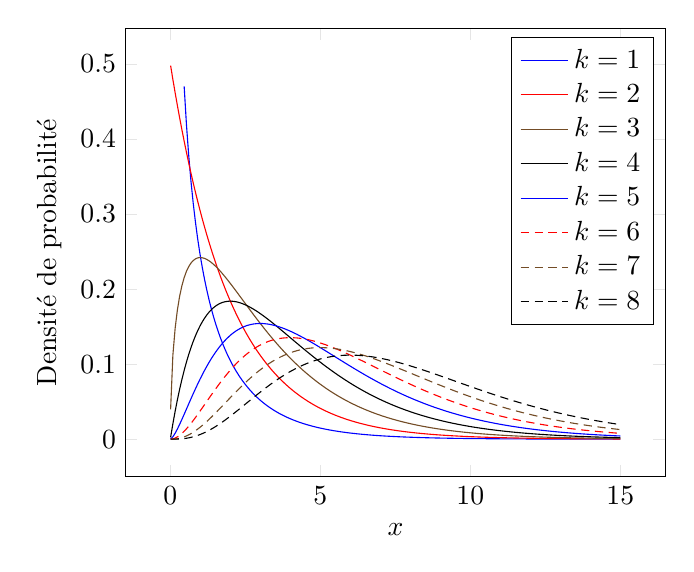
\begin{tikzpicture}[
    declare function={
      gamma(\z)=(2.506628274631*sqrt(1/\z)+ 0.20888568*(1/\z)^(1.5)+ 0.00870357*(1/\z)^(2.5)- (174.2106599*(1/\z)^(3.5))/25920- (715.6423511*(1/\z)^(4.5))/1244160)*exp((-ln(1/\z)-1)*\z);},
    declare function={
        chisq(\x,\k) = (\x)^(\k/2-1) * exp(-\x/2) / (2^(\k/2)) / gamma(\k/2);
    }
]
\begin{axis}[
  xlabel = $x$,
  ylabel = {Densité de probabilité},
  samples = 200,
  restrict y to domain = 0:0.5,
  domain = 0.01:15,
  legend cell align=left]
    \foreach \k in {1,...,8} {
      \addplot+[mark={}] {chisq(x,\k)}; \addlegendentryexpanded{$k=\k$}}
  \end{axis}
\end{tikzpicture}

  \end{center}


\end{frame}


\begin{frame}
  \frametitle{Loi de Student}

  \begin{defn}{}
    Soient $Z$ une variable aléatoire normale centrée réduite et une variable aléatoire $U\perp Z$ distribuéesuivant la loi du $\chi^2$ à $k$ degrés de liberté. Alors
    \[
      X = \frac{Z}{\sqrt{\nicefrac{U}{k}}}
    \]
    suit une loi de Student à $k$ degrés de liberté, notée $t_k$.
  \end{defn}

  \bigskip

  \begin{prop}\label{prop:student}
    La fonction de densité de probabilité de $X\sim t_k$,
    avec $k\in\mathbb N$, est~:
    \[
      f_X(x) =
      \frac{1}{\sqrt{k\pi}}\frac{\Gamma(\frac{k+1}{2})}{\Gamma(\frac{k}{2})}\left(1+\frac{x^2}{k}\right)^{-\frac{k+1}{2}}
    \]
    pour tout $x\in\mathbb R$, où $\Gamma(z) = \int_0^{\infty}t^{z-1}e^{-t}\mathrm dt$ est la
    fonction Gamma. On a $\mathbb E\left[ X \right]=0$ si $k>1$ et $\mathbb V\left[ X \right] = \frac{k}{k-2}$ si $k>2$. La loi de student converge vers la loi normale si $k$ tend vers l'infini.
  \end{prop}

\end{frame}


\begin{frame}
  \frametitle{Loi de Student}

  \bigskip

  \begin{center}
    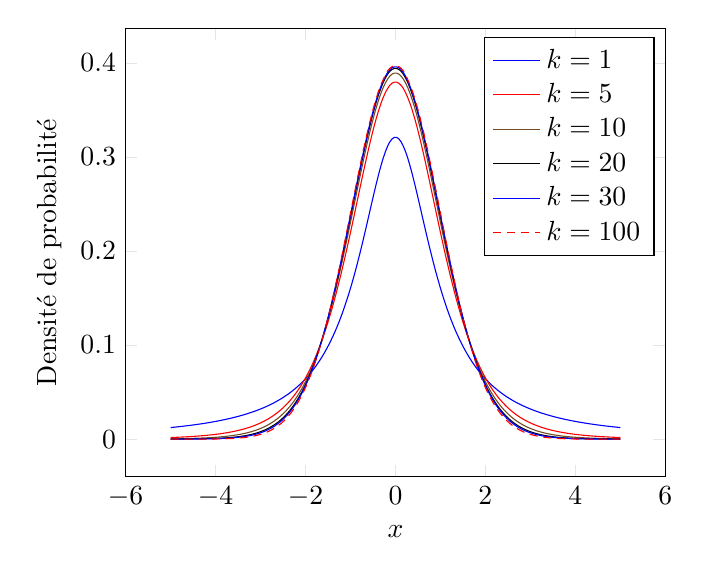
\begin{tikzpicture}[
    declare function={
      gamma(\z)=(2.506628274631*sqrt(1/\z)+ 0.20888568*(1/\z)^(1.5)+ 0.00870357*(1/\z)^(2.5)- (174.2106599*(1/\z)^(3.5))/25920- (715.6423511*(1/\z)^(4.5))/1244160)*exp((-ln(1/\z)-1)*\z);},
    declare function={
      student(\x,\k) = (1/sqrt(3.14159265359*\k))*gamma((\k+1)/2)/gamma(\k/2)*(1+\x*\x/\k)^(-(\k+1)/2);}
]
\begin{axis}[
  xlabel = $x$,
  ylabel = {Densité de probabilité},
  samples = 200,
  restrict y to domain = 0:0.5,
  domain = -5:5,
  legend cell align=left]
    \foreach \k in {1, 5, 10, 20, 30, 100} {
      \addplot+[mark={}] {student(x,\k)}; \addlegendentryexpanded{$k=\k$}}
  \end{axis}
\end{tikzpicture}

  \end{center}


\end{frame}



\begin{frame}
  \frametitle{Loi de Fisher}

  \begin{defn}{}
    Soient $U\sim\chi^2(p)$ et $V\sim\chi^2(q)$, avec  $U\perp V$. $X = \frac{\nicefrac{U}{p}}{\nicefrac{V}{q}}$ une variable aléatoire réelle distribuée selon la loi de Fisher de degrés de liberté $p$ et $q$. On note la distribution de Fisher~: $F(p,q)$.
  \end{defn}

  \bigskip

  \begin{prop}\label{prop:fisher}
    La fonction de densité de probabilité de $X\sim F(p,q)$,
    avec $(p,q)\in\mathbb N^{\star}\times \mathbb N^{\star}$, est~:
    \[
      f_X(x) = \frac{\left( \frac{px}{px+q} \right)^{\frac{p}{2}}\left( 1-\frac{px}{px+q} \right)^{\frac{q}{2}}}{x B\left(\frac{p}{2},\frac{q}{2}\right)}
    \]
    pour tout $x\in\mathbb R_+$, où $B(\alpha,\beta) = \int_0^1t^{\alpha-1}(1-t)^{\beta-1}\mathrm dt$ est la
    fonction Beta. On a $\mathbb E\left[ X \right]=\frac{q}{q-2}$ si $q>2$ et $\mathbb V\left[ X \right] = \frac{2q^2\left( p+q-2 \right)}{p\left( q-2 \right)^2\left( q-4 \right)}$ si $q>4$.
  \end{prop}

\end{frame}


\begin{frame}
  \frametitle{Loi de Fisher}

  \bigskip

  \begin{center}
    \input{images/chapitre-1/fisher-snedecor-1.tex}
  \end{center}


\end{frame}


\begin{frame}
  \frametitle{Loi de Fisher}

  \bigskip

  \begin{center}
    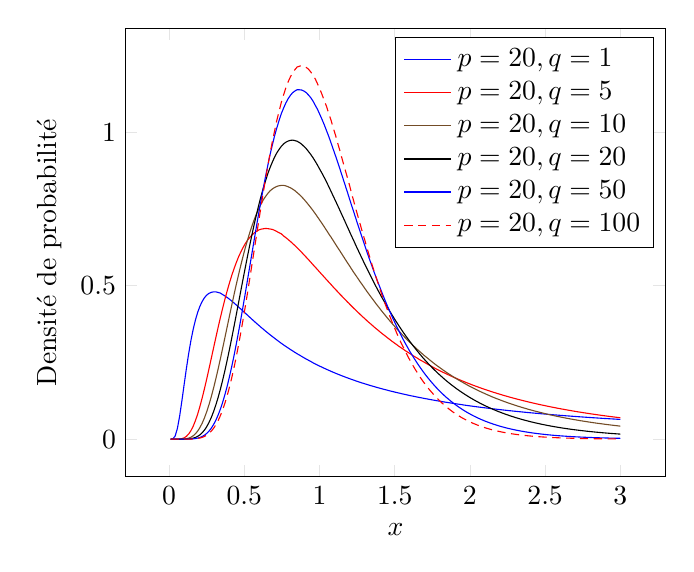
\begin{tikzpicture}[
  declare function={
    gamma(\z)=(2.506628274631*sqrt(1/\z)+ 0.20888568*(1/\z)^(1.5)+ 0.00870357*(1/\z)^(2.5)- (174.2106599*(1/\z)^(3.5))/25920- (715.6423511*(1/\z)^(4.5))/1244160)*exp((-ln(1/\z)-1)*\z);},
  declare function={
    beta(\x,\y)=gamma(\x)*gamma(\y)/gamma(\x+\y);
  },
  declare function={
    fisher(\x,\a,\b) = 1 / beta(\a/2, \b/2) * (\a/\b)^(\a/2) * \x^(\a/2-1) * (1 + \a/\b*\x)^(-(\a + \b)/2);
  }
]
\begin{axis}[
  xlabel = $x$,
  ylabel = {Densité de probabilité},
  samples = 200,
  restrict y to domain = 0:1.5,
  domain = 0.01:3,
  legend cell align=left]
  \foreach \q in {1, 5, 10, 20, 50, 100} {
    \foreach \p in {20} {
      \addplot+[mark={}] {fisher(x,\p, \q}; \addlegendentryexpanded{$p=\p, q=\q$}}}

\end{axis}
\end{tikzpicture}

  \end{center}


\end{frame}


\begin{frame}
  \frametitle{Loi de Fisher}

  \bigskip

  \begin{center}
    \input{images/chapitre-1/fisher-snedecor-3.tex}
  \end{center}


\end{frame}



\end{document}


% Local Variables:
% ispell-check-comments: exclusive
% ispell-local-dictionary: "french"
% TeX-master: t
% End:
